\documentclass[11pt,oneside]{book}
\usepackage{fontspec}
\setmainfont{Noto Serif}
\setsansfont{Noto Sans}
\setmonofont{Noto Sans Mono}
\newfontfamily\proseunicodefont{DejaVu Serif}
\usepackage[margin=1in]{geometry}
\usepackage{microtype}
\usepackage{amsmath,amssymb,amsthm,mathtools,bm}
\usepackage{graphicx}
\usepackage{adjustbox}
\usepackage{xcolor}
\usepackage{booktabs}
\usepackage{array}
\usepackage{longtable}
\usepackage{enumitem}
\usepackage{float}
\usepackage{caption}
\usepackage{hyperref}
\usepackage{fancyhdr}
\usepackage{tikz}
\usetikzlibrary{arrows.meta,positioning,calc,decorations.pathmorphing}

\hypersetup{
  colorlinks=true,
  linkcolor=blue!50!black,
  urlcolor=blue!50!black,
  citecolor=blue!50!black
}

\setlength{\parskip}{0.5em}
\setlength{\parindent}{0pt}
\setlist[itemize]{topsep=0.25em,itemsep=0.2em}
\setlist[enumerate]{topsep=0.25em,itemsep=0.2em}
\setlength{\headheight}{40pt}
\numberwithin{equation}{chapter}

\newtheorem{theorem}{Théorème}[chapter]
\newtheorem{proposition}[theorem]{Proposition}
\newtheorem{lemma}[theorem]{Lemme}
\newtheorem{corollary}[theorem]{Corollaire}
\theoremstyle{definition}
\newtheorem{definition}[theorem]{Définition}
\newtheorem{example}[theorem]{Exemple}
\theoremstyle{remark}
\newtheorem{remark}[theorem]{Remarque}

\providecommand{\ket}[1]{\left\lvert#1\right\rangle}
\providecommand{\bra}[1]{\left\langle#1\right\rvert}
\providecommand{\braket}[2]{\left\langle#1\,\middle|\,#2\right\rangle}
\providecommand{\expect}[1]{\left\langle#1\right\rangle}
\newcommand{\lectureoverview}[1]{\paragraph{Vue d’ensemble.} #1}

\makeatletter
\newcommand{\course@headerfont}{\normalfont\small\itshape}
\newcommand{\course@pagefont}{\normalfont\small}
\newcommand{\course@headerraise}{14pt}
\newlength{\course@headerboxheight}
\setlength{\course@headerboxheight}{\dimexpr\headheight-\course@headerraise-9pt\relax}
\newcommand{\course@leftheadbox}[1]{%
  \raisebox{\course@headerraise}{%
    \parbox[t][\course@headerboxheight][t]{0.82\textwidth}{%
      \raggedright\course@headerfont\strut\MakeUppercase{#1}\strut%
    }%
  }%
}
\newcommand{\course@rightheadbox}[1]{%
  \raisebox{\course@headerraise}{%
    \parbox[t][\course@headerboxheight][t]{0.82\textwidth}{%
      \raggedleft\course@headerfont\strut\MakeUppercase{#1}\strut%
    }%
  }%
}
\renewcommand{\chaptermark}[1]{\markboth{\MakeUppercase{\chaptername\ \thechapter.\ #1}}{}}
\renewcommand{\sectionmark}[1]{\markright{\MakeUppercase{\thesection\hspace{0.4em}#1}}}
\fancyhf{}
\fancyhead[L]{\course@leftheadbox{\leftmark}}
\fancyhead[R]{\course@pagefont\thepage}
\renewcommand{\headrulewidth}{0.5pt}
\pagestyle{fancy}
\fancypagestyle{plain}{%
  \fancyhf{}
  \fancyhead[L]{\course@leftheadbox{\leftmark}}
  \fancyhead[R]{\course@pagefont\thepage}
  \renewcommand{\headrulewidth}{0.5pt}
}
\makeatother

% Video2Book editorial provenance macros
\newenvironment{classroomqa}{%
  \par\medskip\noindent\begin{minipage}{\linewidth}\small\hrule\medskip
}{%
  \medskip\hrule\end{minipage}\par\medskip
}
\newcommand{\audiencequestion}[1]{\noindent\textbf{Question du public.} #1\par\smallskip}
\newcommand{\lecturerresponse}[1]{\noindent\textbf{Réponse.} #1\par}
\newcommand{\lecturetimestamp}[1]{\footnote{Horodatage du cours : #1.}}
\newcommand{\lectureframe}[1]{\par\smallskip{\centering\footnotesize\itshape Image du cours : #1.\par}}
\newcommand{\editorialnote}[1]{\footnote{Précision éditoriale : #1}}

\usepackage{polyglossia}
\setdefaultlanguage{french}
\usepackage{sectsty}
\renewcommand{\contentsname}{Table des matières}
\renewcommand{\chaptername}{Chapitre}
\renewcommand{\figurename}{Figure}
\renewcommand{\tablename}{Tableau}
\renewcommand{\proofname}{Démonstration}
\renewcommand{\bibname}{Références}
\sectionfont{\raggedright}
\subsectionfont{\raggedright}
\makeatletter
\renewcommand{\@pnumwidth}{2.2em}
\renewcommand{\@tocrmarg}{3.2em}
\makeatother
\usepackage{tocloft}
\renewcommand{\cftchapfont}{\small\bfseries}
\renewcommand{\cftchappagefont}{\small\bfseries}
\renewcommand{\cftsecfont}{\small}
\renewcommand{\cftsecpagefont}{\small}
\setlength{\cftsecnumwidth}{3em}
\emergencystretch=6em
\pdfstringdefDisableCommands{\def\proseunicodefont{}}

\geometry{paperwidth=177.6mm,paperheight=252mm,left=16mm,right=16mm,
 top=18mm,bottom=18mm,includeheadfoot,headheight=28pt,headsep=7mm,footskip=9mm}
\usepackage{scrextend}
\changefontsizes[17pt]{12pt}
\raggedbottom
\renewenvironment{classroomqa}{\par\medskip\begingroup}{\par\endgroup\medskip}
\fancyhf{}
\setlength{\headwidth}{\textwidth}
\fancyhead[L]{\parbox{\textwidth}{\raggedright\fontsize{9}{11}\selectfont\nouppercase{\leftmark}}}
\fancyfoot[C]{\small\thepage}
\renewcommand{\headrulewidth}{0.3pt}
\fancypagestyle{plain}{\fancyhf{}\fancyfoot[C]{\small\thepage}\renewcommand{\headrulewidth}{0pt}}

\graphicspath{{../../../generated_course_notes/supplementary/advanced_quantum_mechanics/2013_fall/figures/}{../../../generated_course_notes/supplementary/advanced_quantum_mechanics/2013_fall/assets/}}
\begin{document}
\frontmatter
\hypersetup{pageanchor=false}
\begin{titlepage}
\thispagestyle{empty}
\begin{tikzpicture}[remember picture,overlay]
  \node[anchor=center,inner sep=0] at (current page.center) {%
    \includegraphics[height=\paperheight,keepaspectratio]{../../../generated_course_notes/supplementary/advanced_quantum_mechanics/2013_fall/assets/cover-art.png}%
  };
  \node[
    anchor=north west,
    align=left,
    text width=0.78\paperwidth,
    fill=white,
    fill opacity=0.9,
    rounded corners=8pt,
    inner xsep=10pt,
    inner ysep=8pt
  ] at ([xshift=0.08\paperwidth,yshift=-0.06\paperheight]current page.north west) {%
    {\fontsize{30}{33}\selectfont\bfseries\color{black!88} Mécanique quantique avancée\\[0.85em]}
    {\large\color{black!72} Édition française / automne 2013}
  };
  \node[
    anchor=south west,
    align=left,
    text width=0.68\paperwidth,
    fill=white,
    fill opacity=0.82,
    text opacity=1,
    rounded corners=6pt,
    inner sep=12pt
  ] at ([xshift=0.08\paperwidth,yshift=0.08\paperheight]current page.south west) {%
    {\normalsize\color{black!78} Cours originaux : Leonard Susskind\\[0.35em]}
    {\small\color{black!72} Édition d’accompagnement : \href{https://lazying.art}{LazyingArt LLC} / \href{https://github.com/lachlanchen/Video2Book}{Video2Book}}
  };
\end{tikzpicture}
\mbox{}
\end{titlepage}
\hypersetup{pageanchor=true}

\clearpage
\chapter{À propos de ces notes}
Ces notes d’accompagnement, éditées de manière indépendante, suivent les cours de Leonard Susskind. Elles ont été reconstituées à partir de transcriptions automatiques, de sous-titres et d’une sélection d’images du tableau, puis vérifiées à l’aide des sources disponibles. Elles ne constituent pas un manuscrit original du professeur Susskind et n’ont été ni relues ni approuvées par lui.

Cette édition a été préparée par \href{https://lazying.art}{LazyingArt LLC} au moyen du processus open source \href{https://github.com/lachlanchen/Video2Book}{Video2Book}. Les transcriptions automatiques restent disponibles séparément et peuvent comporter des erreurs de reconnaissance. Les précisions éditoriales et les reconstitutions non triviales sont signalées dans des notes de bas de page.
\clearpage
\tableofcontents
\mainmatter
\chapter{Vecteurs d’état, évolution unitaire et symétrie de translation}
\providecommand{\ket}[1]{\left\lvert#1\right\rangle}
\providecommand{\bra}[1]{\left\langle#1\right\rvert}

Après une interruption de deux trimestres, une révision rapide de la mécanique quantique est utile. Elle ne peut toutefois pas occuper tout le trimestre. Nous allons étudier l’application de la mécanique quantique aux problèmes pour lesquels elle a été développée à l’origine : les atomes, les électrons et les particules apparentées, ainsi que les photons.

Nous commencerons par les atomes. Comment peuvent-ils venir avant les électrons, alors que les électrons sont des constituants des atomes ? Au début, il suffit de connaître assez de mécanique électronique pour écrire les équations de base de l’atome d’hydrogène. Nous pourrons ensuite étudier plus en détail les particules apparentées aux électrons. Dans toutes ces applications, la symétrie sera un outil récurrent : nous examinerons comment les symétries sont représentées en mécanique quantique et ce qu’elles impliquent pour un système.

\section{États, observables et orthogonalité}

En mécanique classique, un état est représenté par un point de l’espace des phases. En mécanique quantique, il est représenté par un vecteur d’un espace vectoriel complexe. Il s’agit d’un vecteur abstrait, et non d’une flèche dans l’espace ordinaire à trois dimensions. Les vecteurs d’état peuvent être additionnés et multipliés par des nombres complexes, et l’espace qui les contient n’a pas besoin d’être de dimension finie particulière.

La notation de Dirac désigne un vecteur d’état par un ket,
\begin{equation}
\ket{\psi},
\end{equation}
et lui associe un bra,
\begin{equation}
\bra{\psi}.
\end{equation}
Les bras et les kets sont liés par la conjugaison hermitienne. La combinaison d’un bra et d’un ket donne un produit scalaire,
\begin{equation}
\langle\phi|\psi\rangle,
\end{equation}
qui est en général un nombre complexe.

Une observable est une grandeur susceptible d’être mesurée : la position, la quantité de mouvement, l’énergie ou toute autre grandeur mesurable. En mécanique quantique, une observable est représentée par un opérateur linéaire hermitien \(A\),
\begin{equation}
A^\dagger=A.
\end{equation}
L’hermiticité est l’analogue, pour les opérateurs, de la réalité. En particulier, les valeurs propres d’un opérateur hermitien sont réelles.

Un vecteur propre de \(A\) vérifie
\begin{equation}
A\ket{\alpha}=\alpha\ket{\alpha}.
\end{equation}
Les valeurs propres possibles sont les résultats possibles d’une mesure de \(A\). Par exemple, si une observable ne peut prendre que les valeurs \(1\), \(3\) ou \(7\), celles-ci sont ses valeurs propres. Ses vecteurs propres sont les états pour lesquels le résultat est déterminé, plutôt que statistique. Dans l’état \(\ket{\alpha}\), une mesure de \(A\) donne certainement \(\alpha\).

Le produit scalaire exprime une importante relation logique entre les états. Supposons qu’il existe une mesure permettant de distinguer avec certitude \(\ket{\phi}\) de \(\ket{\psi}\). Les états sont alors orthogonaux :
\begin{equation}
\langle\phi|\psi\rangle=0.
\end{equation}
L’orthogonalité signifie que les états sont physiquement distinguables sans ambiguïté. Pour un état normalisé,
\begin{equation}
\langle\psi|\psi\rangle=1.
\end{equation}

\section{Une particule dans la représentation de position}

Considérons d’abord une particule se déplaçant sur une droite. Sa position \(x\) est une observable. À chaque position possible \(x_0\) correspond un état \(\ket{x_0}\) dans lequel une mesure de position donne certainement \(x_0\).

Des états associés à des positions différentes sont distinguables et donc orthogonaux :
\begin{equation}
x\neq x'
\quad\Longrightarrow\quad
\langle x'|x\rangle=0.
\end{equation}
Pour un état arbitraire \(\ket{\psi}\), son recouvrement avec un état de position définit la fonction d’onde :
\begin{equation}
\psi(x)=\langle x|\psi\rangle.
\end{equation}
C’est la représentation de position du vecteur d’état.

La fonction d’onde n’est pas elle-même une probabilité. Elle peut être positive, négative, imaginaire ou entièrement complexe. La densité de probabilité de position est
\begin{equation}
P(x)=\psi^*(x)\psi(x)=|\psi(x)|^2.
\end{equation}
Le produit est non négatif, comme doit l’être une densité de probabilité. Pour une fonction d’onde normalisée,
\begin{equation}
\int_{-\infty}^{\infty}dx\,|\psi(x)|^2=1.
\end{equation}

Dans la représentation de position, l’opérateur position agit par multiplication :
\begin{equation}
(\hat x\psi)(x)=x\psi(x).
\end{equation}
Ses fonctions propres sont des fonctions idéalisées, concentrées en un point. Elles sont décrites formellement par des distributions de Dirac : des pics très étroits centrés sur la valeur propre de position. Leur définition précise au sens des distributions n’est pas nécessaire pour cette révision.

En trois dimensions, la position a trois composantes, \(x\), \(y\) et \(z\), et un état de position représente un point de l’espace tridimensionnel. Deux états de ce type sont orthogonaux dès que leurs points diffèrent d’au moins une coordonnée. Nous conserverons généralement la notation unidimensionnelle, en sous-entendant son extension correspondante à trois dimensions.

\section{Quantité de mouvement et états de quantité de mouvement déterminée}

À chaque composante de la position correspond une composante de la quantité de mouvement. Dans la représentation de position, l’opérateur quantité de mouvement selon l’axe \(x\) est
\begin{equation}
\hat p_x=-i\hbar\frac{d}{dx}.
\end{equation}
Ainsi, un opérateur hermitien abstrait peut aussi être considéré concrètement comme une opération sur les fonctions d’onde.

Un état de quantité de mouvement déterminée \(p_0\) vérifie l’équation aux valeurs propres
\begin{equation}
\hat p_x\psi_{p_0}(x)=p_0\psi_{p_0}(x).
\end{equation}
En substituant la forme différentielle de \(\hat p_x\), on obtient
\begin{equation}
-i\hbar\frac{d\psi_{p_0}(x)}{dx}
=p_0\psi_{p_0}(x).
\end{equation}
La dérivée de la fonction d’onde est proportionnelle à la fonction d’onde elle-même ; la solution est donc de forme exponentielle :
\begin{equation}
\psi_{p_0}(x)\propto
\exp\left(\frac{ip_0x}{\hbar}\right).
\end{equation}

\begin{classroomqa}
\lecturetimestamp{00:24:26}
\audiencequestion{Cette équation différentielle est-elle vérifiée par toute fonction d’onde ?}
\lecturerresponse{Non. C’est l’équation aux valeurs propres d’un état de quantité de mouvement déterminée. La plupart des fonctions d’onde ne la vérifient pas ; elle sélectionne les fonctions propres de quantité de mouvement.}
\end{classroomqa}

La distinction entre les états propres de position et ceux de quantité de mouvement est nette. Une fonction propre de position est concentrée en un point. Le module d’une fonction propre de quantité de mouvement est
\begin{equation}
\left|\exp\left(\frac{ip_0x}{\hbar}\right)\right|^2=1.
\end{equation}
Il est donc constant sur toute la droite. En ce sens idéalisé, une quantité de mouvement déterminée implique une incertitude complète sur la position ; de même, une position déterminée implique une incertitude complète sur la quantité de mouvement. C’est le cas limite de la relation d’incertitude position--quantité de mouvement.

\begin{classroomqa}
\lecturetimestamp{00:26:36}
\audiencequestion{Si la quantité de mouvement est connue et vaut \(p_0\), pourquoi subsiste-t-il une distribution de probabilité ?}
\lecturerresponse{La quantité affichée concerne une mesure de position, et non une autre mesure de quantité de mouvement. La position et la quantité de mouvement sont des observables différentes. Pour l’état propre idéalisé de quantité de mouvement, le module de l’amplitude de position est constant sur toute la droite. Les amplitudes de quantité de mouvement relèvent de la représentation de quantité de mouvement et sont reliées à la fonction d’onde de position par une transformée de Fourier.}
\end{classroomqa}

\begin{classroomqa}
\lecturetimestamp{00:28:02}
\audiencequestion{À quoi ressemble la probabilité de position lorsque la fonction d’onde est une distribution de Dirac ?}
\lecturerresponse{Elle est concentrée à la position spécifiée. Ce pic idéalisé exprime la certitude de la position.}
\end{classroomqa}

\editorialnote{Les états propres exacts de position et de quantité de mouvement sont des états généralisés. Une distribution de Dirac et une onde plane ne sont pas des fonctions d’onde ordinaires, normalisables au carré et intégrables sur toute la droite ; de plus, le carré littéral d’une distribution de Dirac n’est pas une distribution ordinaire. Les énoncés ci-dessus portent sur leur localisation idéalisée et leur module constant.}

On peut considérer formellement une fonction d’onde comme un vecteur ayant une composante pour chaque valeur de \(x\). Contrairement à un vecteur colonne ordinaire de dimension finie, elle possède toutefois une infinité continue de composantes.

\begin{classroomqa}
\lecturetimestamp{00:28:53}
\audiencequestion{Les vecteurs d’état sont-ils représentés par des vecteurs colonnes ?}
\lecturerresponse{Ils peuvent l’être, mais il est malcommode d’écrire une fonction d’onde de position sous la forme d’un vecteur colonne ordinaire, car \(x\) prend un continuum de valeurs. On peut la considérer formellement comme un vecteur colonne continu, et considérer le bra correspondant comme un vecteur ligne continu.}
\end{classroomqa}

\section{Évolution temporelle et unitarité}

Comment un état évolue-t-il au cours du temps ? L’évolution temporelle est une transformation dans l’espace des états. Désignons par \(U(t)\) l’évolution pendant un intervalle de temps écoulé \(t\). Alors,
\begin{equation}
U(t)\ket{\psi(t_1)}=\ket{\psi(t_1+t)}.
\end{equation}
En particulier,
\begin{equation}
\ket{\psi(t)}=U(t)\ket{\psi(0)},
\qquad
U(0)=\mathbf 1.
\end{equation}

La condition imposée à \(U(t)\) découle de la conservation de l’information. Si deux états initiaux sont distinguables, l’évolution temporelle ne doit pas effacer cette distinction. Des états orthogonaux doivent rester orthogonaux. Plus généralement, le produit scalaire de deux états quelconques est conservé :
\begin{equation}
\langle U(t)\phi|U(t)\psi\rangle
=\langle\phi|\psi\rangle.
\end{equation}
Puisque
\begin{equation}
\langle U(t)\phi|U(t)\psi\rangle
=\langle\phi|U^\dagger(t)U(t)|\psi\rangle,
\end{equation}
la conservation de tous les produits scalaires exige
\begin{equation}
U^\dagger(t)U(t)=\mathbf 1.
\end{equation}
Un opérateur qui vérifie cette équation est unitaire.

\begin{classroomqa}
\lecturetimestamp{00:36:36}
\audiencequestion{La conservation de chaque produit scalaire est-elle une condition plus forte que la simple conservation de l’orthogonalité ?}
\lecturerresponse{Pour les transformations linéaires des états considérées ici, la conservation de l’orthogonalité entraîne celle des produits scalaires. Les rotations ordinaires en donnent l’analogie familière : elles conservent l’orthogonalité et les produits scalaires.}
\end{classroomqa}

\editorialnote{Au sens strict, la conservation de l’orthogonalité seule autorise un facteur d’échelle global non nul. La conservation de la norme, déjà exigée pour l’évolution temporelle physique, élimine cette liberté et entraîne la conservation des produits scalaires.}

Il ne faut pas confondre les opérateurs unitaires avec les observables hermitiennes. La position et la quantité de mouvement sont hermitiennes, mais ne sont généralement pas unitaires. Les valeurs propres d’un opérateur unitaire sont des phases, c’est-à-dire des nombres de la forme \(e^{i\theta}\) situés sur le cercle unité.

\begin{classroomqa}
\lecturetimestamp{00:38:12}
\audiencequestion{Quel est un exemple de transformation non unitaire ?}
\lecturerresponse{Les opérateurs position et quantité de mouvement en sont des exemples : ce sont des observables hermitiennes, mais ils ne sont pas unitaires. Un opérateur unitaire a des valeurs propres de module unité ; ses valeurs propres sont donc des phases.}
\end{classroomqa}

\section{Le Hamiltonien et l’équation de Schr\"odinger}

On suppose que l’évolution temporelle est continue. Sur un intervalle très court \(\epsilon\), l’opérateur d’évolution doit donc être proche de l’identité :
\begin{equation}
U(\epsilon)=\mathbf 1+\epsilon G+\mathcal O(\epsilon^2).
\end{equation}
En utilisant l’unitarité,
\begin{align}
U^\dagger(\epsilon)U(\epsilon)
&=
\left(\mathbf 1+\epsilon G^\dagger\right)
\left(\mathbf 1+\epsilon G\right)
+\mathcal O(\epsilon^2)
\\
&=
\mathbf 1+\epsilon(G^\dagger+G)
+\mathcal O(\epsilon^2).
\end{align}
Au premier ordre,
\begin{equation}
G^\dagger=-G.
\end{equation}
Ainsi, \(G\) est antihermitien. On peut l’écrire
\begin{equation}
G=-\frac{i}{\hbar}H,
\end{equation}
où \(H\) est hermitien :
\begin{equation}
H^\dagger=H.
\end{equation}
L’opérateur infinitésimal d’évolution temporelle est donc
\begin{equation}
U(\epsilon)
=
\mathbf 1-\frac{i\epsilon}{\hbar}H
+\mathcal O(\epsilon^2).
\end{equation}
L’opérateur hermitien \(H\) est le Hamiltonien.

\begin{classroomqa}
\lecturetimestamp{00:45:48}
\audiencequestion{Pourquoi peut-on négliger le terme \(\epsilon^2\) ?}
\lecturerresponse{Le calcul est mené de façon cohérente au premier ordre en \(\epsilon\). Un calcul au second ordre devrait inclure tous les termes du second ordre, y compris le terme proportionnel à \(-\epsilon^2H^2/(2\hbar^2)\). L’approximation vient de l’expression tronquée de \(U(\epsilon)\), et non de l’hermiticité de \(H\).}
\end{classroomqa}

On peut construire un intervalle de temps fini à partir d’un grand nombre de petits intervalles. Découpons \(t\) en \(N\) pas de longueur \(t/N\). La répétition de la transformation infinitésimale donne
\begin{equation}
U(t)
=
\lim_{N\to\infty}
\left(
\mathbf 1-\frac{itH}{N\hbar}
\right)^N
=
\exp\left(-\frac{iHt}{\hbar}\right).
\end{equation}
L’exponentielle est la version finie de la transformation infinitésimale.

Faisons maintenant évoluer un état de \(t\) à \(t+\epsilon\) :
\begin{align}
\ket{\psi(t+\epsilon)}
&=
U(\epsilon)\ket{\psi(t)}
\\
&=
\left(
\mathbf 1-\frac{i\epsilon}{\hbar}H
\right)\ket{\psi(t)}
+\mathcal O(\epsilon^2).
\end{align}
En soustrayant \(\ket{\psi(t)}\), en divisant par \(\epsilon\), puis en prenant la limite, on obtient
\begin{equation}
\frac{d}{dt}\ket{\psi(t)}
=
-\frac{i}{\hbar}H\ket{\psi(t)}.
\end{equation}
De façon équivalente,
\begin{equation}
i\hbar\frac{d}{dt}\ket{\psi(t)}
=
H\ket{\psi(t)}.
\end{equation}
C’est l’équation de Schr\"odinger dépendant du temps. Dans la représentation de position, elle devient
\begin{equation}
i\hbar\frac{\partial}{\partial t}\psi(x,t)
=
H\psi(x,t),
\end{equation}
où \(H\) agit comme un opérateur sur la fonction d’onde.

L’équation de Schr\"odinger indépendante du temps est l’équation aux valeurs propres du Hamiltonien :
\begin{equation}
H\ket{E}=E\ket{E}.
\end{equation}
Les valeurs propres \(E\) sont les énergies mesurables possibles, ou niveaux d’énergie. Le même Hamiltonien détermine donc à la fois les énergies permises et l’évolution de l’état.

Si l’état initial est un état propre d’énergie, son évolution est
\begin{equation}
\ket{E;t}
=
\exp\left(-\frac{iEt}{\hbar}\right)\ket{E}.
\end{equation}
Il reste le même vecteur propre d’énergie et acquiert seulement une phase.\footnote{Le signe moins est fixé par la dérivation précédente de \(U(t)=\exp(-iHt/\hbar)\). Une formulation orale ultérieure de la phase donne le signe opposé et est incompatible avec cette dérivation.}

\begin{classroomqa}
\lecturetimestamp{01:01:05}
\audiencequestion{Comment un vecteur propre d’énergie évolue-t-il selon l’équation de Schr\"odinger dépendant du temps ?}
\lecturerresponse{Conservons le ket. Puisque \(H\ket{E}=E\ket{E}\), l’évolution temporelle multiplie le vecteur propre d’énergie par une phase déterminée par son énergie : \(\exp(-iEt/\hbar)\).}
\end{classroomqa}

\section{Qu’appelle-t-on une symétrie ?}

L’évolution temporelle est une transformation unitaire dans l’espace des états. Les transformations de symétrie constituent une autre classe importante.

La symétrie de rotation joue un rôle central en physique atomique. Dans un atome d’hydrogène, l’électron se déplace dans le potentiel coulombien central. Une rotation du système de coordonnées ne modifie pas les équations ; une rotation physique de l’atome laisse également un atome d’hydrogène régi par les mêmes équations. L’état peut changer sous l’effet de la rotation, mais pas la loi dynamique.

La translation en fournit un autre exemple. Un système isolé dans le vide devrait se comporter de la même façon lorsque toutes ses parties sont déplacées d’une même quantité. Cette précision est importante. Si un four est présent et que seul le système est rapproché de celui-ci, le système peut se comporter différemment ; le four brise cette symétrie de translation. Si le système et le four sont tous deux translatés ensemble, leur relation initiale est rétablie.

Toute opération n’est pas une symétrie. Comprimer un cristal de sel gemme d’un facteur deux modifie généralement son comportement. La compression est une transformation bien définie, mais elle n’est généralement pas une symétrie.

Une symétrie est donc une opération sur les états qui préserve la forme de la dynamique. Désignons-la par \(V\). Elle doit préserver la distinguabilité : deux états orthogonaux doivent rester orthogonaux après la transformation. Par conséquent,
\begin{equation}
V^\dagger V=\mathbf 1,
\end{equation}
et \(V\) est unitaire.

\section{Les symétries commutent avec l’évolution temporelle}

Supposons qu’un état initial \(\ket{\psi_1}\) évolue vers \(\ket{\psi_2}\) :
\begin{equation}
\ket{\psi_2}=U(t)\ket{\psi_1}.
\end{equation}
Appliquons une symétrie candidate \(V\) aux deux états :
\begin{equation}
\ket{\psi_1'}=V\ket{\psi_1},
\qquad
\ket{\psi_2'}=V\ket{\psi_2}.
\end{equation}
Si \(V\) est une symétrie de la dynamique, l’état initial transformé doit évoluer vers l’état final transformé :
\begin{equation}
\ket{\psi_2'}=U(t)\ket{\psi_1'}.
\end{equation}
En substituant les définitions, on obtient
\begin{equation}
VU(t)\ket{\psi_1}
=
U(t)V\ket{\psi_1}.
\end{equation}
Cette relation doit être vérifiée pour tout état initial. Par conséquent,
\begin{equation}
VU(t)=U(t)V.
\end{equation}

Les deux voies équivalentes peuvent être représentées par un diagramme commutatif.\footnote{Le diagramme reconstitue l’argument des deux voies développé entre les repères temporels 01:10:30 et 01:16:34.}\begin{figure}\centering
\begin{tikzpicture}[>=Stealth]
\node (a) at (0,0) {$\ket{\psi_1}$};
\node (b) at (4.2,0) {$\ket{\psi_2}=U(t)\ket{\psi_1}$};
\node (c) at (0,-2.0) {$V\ket{\psi_1}$};
\node (d) at (4.2,-2.0) {$V\ket{\psi_2}=U(t)V\ket{\psi_1}$};

\draw[->] (a) -- node[above] {$U(t)$} (b);
\draw[->] (c) -- node[below] {$U(t)$} (d);
\draw[->] (a) -- node[left] {$V$} (c);
\draw[->] (b) -- node[right] {$V$} (d);
\end{tikzpicture}\caption{Une opération de symétrie et l’évolution temporelle conduisent au même état final, quel que soit l’ordre dans lequel elles sont appliquées.}\end{figure}

\begin{classroomqa}
\lecturetimestamp{01:16:38}
\audiencequestion{La symétrie doit-elle commuter avec l’évolution temporelle pour toutes les durées ?}
\lecturerresponse{Oui. Une symétrie de la dynamique doit satisfaire la condition de commutation pour l’évolution temporelle complète.}
\end{classroomqa}

\begin{classroomqa}
\lecturetimestamp{01:17:13}
\audiencequestion{Cela signifie-t-il que l’on peut effectuer une rotation puis attendre, ou attendre puis effectuer une rotation ?}
\lecturerresponse{Exactement. Si la rotation est une symétrie, les deux ordres donnent le même état final transformé.}
\end{classroomqa}

Pour un petit intervalle de temps,
\begin{equation}
U(\epsilon)
=
\mathbf 1-\frac{i\epsilon}{\hbar}H
+\mathcal O(\epsilon^2).
\end{equation}
La condition de commutation devient
\begin{equation}
V\left(
\mathbf 1-\frac{i\epsilon}{\hbar}H
\right)
=
\left(
\mathbf 1-\frac{i\epsilon}{\hbar}H
\right)V
+\mathcal O(\epsilon^2).
\end{equation}
Les termes d’identité s’annulent, ce qui laisse
\begin{equation}
VH=HV,
\end{equation}
soit
\begin{equation}
[V,H]=0.
\end{equation}
Ainsi, une opération unitaire est une symétrie de la dynamique si et seulement si elle commute avec le Hamiltonien.

\begin{classroomqa}
\lecturetimestamp{01:19:29}
\audiencequestion{Pourquoi l’opérateur de symétrie \(V\) doit-il être unitaire ?}
\lecturerresponse{Une symétrie doit préserver les distinctions logiques entre les états. Elle ne devrait pas transformer deux états orthogonaux mutuellement exclusifs en états qui ne seraient plus distinguables. La préservation de ces relations exige une transformation unitaire.}
\end{classroomqa}

Un opérateur sans dépendance explicite en temps qui commute avec \(H\) est conservé. Cela relie la symétrie à la conservation. En mécanique classique, cette relation s’exprime par le théorème de Noether. Dans la formulation quantique considérée ici, le critère central est le commutateur avec le Hamiltonien.

\section{Symétries discrètes et continues}

Les symétries peuvent être discrètes ou continues. Une réflexion dans un miroir est discrète : elle échange la gauche et la droite, sans qu’il existe entre les deux une suite de réflexions infinitésimales. L’échange de deux particules identiques est une autre opération discrète. Le retournement d’un objet à deux faces non marquées en donne un exemple du même type.

Les rotations sont continues. Une rotation de \(90^\circ\) peut être construite à partir de nombreuses petites rotations autour du même axe. Les translations spatiales sont continues pour la même raison : un déplacement fini peut être construit à partir d’une multitude de déplacements infinitésimaux.

Cette décomposition en petites transformations confère une forme particulière aux symétries continues. Au voisinage de l’identité, écrivons
\begin{equation}
V(\epsilon)
=
\mathbf 1-i\epsilon G+\mathcal O(\epsilon^2),
\end{equation}
où \(\epsilon\) paramètre la transformation. L’unitarité implique
\begin{equation}
G^\dagger=G.
\end{equation}
L’opérateur hermitien \(G\) est appelé le générateur de la symétrie.

Si la transformation est une symétrie, alors
\begin{equation}
[H,V(\epsilon)]=0.
\end{equation}
En développant au premier ordre, on obtient
\begin{equation}
[H,G]=0.
\end{equation}
Les symétries continues sont donc engendrées par des opérateurs hermitiens qui commutent avec le Hamiltonien. Ces générateurs sont des grandeurs conservées.

Le mot ``engendrée'' a ici un sens concret. Une transformation finie est construite en appliquant plusieurs fois la transformation infinitésimale, tout comme l’évolution temporelle finie est construite à partir de nombreux petits pas de temps.

\section{Symétrie de translation et quantité de mouvement}

Considérons la translation active d’une fonction d’onde vers la droite d’une distance \(\epsilon\). Si la fonction d’onde initiale est centrée en \(x_0\), la fonction d’onde translatée doit être centrée en \(x_0+\epsilon\). Sa valeur à la coordonnée \(x\) est donc celle de l’ancienne fonction d’onde évaluée en \(x-\epsilon\) :
\begin{equation}
(T(\epsilon)\psi)(x)=\psi(x-\epsilon).
\end{equation}
Pour un petit déplacement,
\begin{equation}
\psi(x-\epsilon)
=
\psi(x)-\epsilon\frac{d\psi(x)}{dx}
+\mathcal O(\epsilon^2).
\end{equation}
On a donc
\begin{equation}
T(\epsilon)
=
\mathbf 1-\epsilon\frac{d}{dx}
+\mathcal O(\epsilon^2).
\end{equation}
En utilisant
\begin{equation}
\hat p_x=-i\hbar\frac{d}{dx},
\qquad
\frac{d}{dx}=\frac{i}{\hbar}\hat p_x,
\end{equation}
la translation infinitésimale devient
\begin{equation}
T(\epsilon)
=
\mathbf 1-\frac{i\epsilon}{\hbar}\hat p_x
+\mathcal O(\epsilon^2).
\end{equation}
La translation finie correspondante est
\begin{equation}
T(\epsilon)
=
\exp\left(-\frac{i\epsilon}{\hbar}\hat p_x\right).
\end{equation}
Avec la convention \(V(\epsilon)=\mathbf 1-i\epsilon G+\cdots\), le paramètre de translation dimensionné donne
\begin{equation}
G_{\mathrm{trans}}=\frac{\hat p_x}{\hbar}.
\end{equation}
De façon équivalente, on dit que la quantité de mouvement est le générateur des translations spatiales lorsque le facteur \(\hbar\) apparaît explicitement dans l’exponentielle.

\begin{classroomqa}
\lecturetimestamp{01:34:08}
\audiencequestion{Un signe moins a-t-il été perdu dans la dérivation de la translation ?}
\lecturerresponse{La question vient du sens attribué au déplacement de la fonction d’onde. Une translation active vers la droite est représentée par \(\psi(x-\epsilon)\), et non par \(\psi(x+\epsilon)\). Avec cette correction, on obtient \(T(\epsilon)=\mathbf 1-i\epsilon\hat p_x/\hbar+\cdots\).}
\end{classroomqa}

La conservation de la quantité de mouvement dépend du Hamiltonien. Pour une particule libre se déplaçant à une dimension,
\begin{equation}
H=\frac{\hat p_x^2}{2m}.
\end{equation}
Tout opérateur commutant avec toute fonction de lui-même,
\begin{equation}
[H,\hat p_x]=0.
\end{equation}
le Hamiltonien de la particule libre est invariant par translation, et \(\hat p_x\) est conservé. Physiquement, la particule se comporte de la même façon quel que soit le choix de sa position initiale. La translation de la condition initiale translate simplement l’ensemble du mouvement.

En trois dimensions,
\begin{equation}
H
=
\frac{\hat p_x^2+\hat p_y^2+\hat p_z^2}{2m}.
\end{equation}
Chaque composante de la quantité de mouvement commute avec \(H\) :
\begin{equation}
[H,\hat p_x]=[H,\hat p_y]=[H,\hat p_z]=0.
\end{equation}
Il existe une symétrie de translation distincte dans chaque direction spatiale. La quantité de mouvement est à la fois la grandeur conservée et le générateur associé à ces translations.

Le cas suivant est celui de la symétrie de rotation. Les rotations sont plus complexes, car les rotations autour d’axes différents ne commutent généralement pas : une rotation de \(x\) suivie d’une rotation de \(y\) ne donne pas le même résultat que l’ordre inverse. Il en découle des générateurs de symétrie qui ne commutent pas, ainsi que la structure de groupe des rotations.

\chapter{Symétrie, dégénérescence et échelles de moment cinétique}
\providecommand{\ket}[1]{\left\lvert#1\right\rangle}

\section{Symétries et niveaux d’énergie dégénérés}

Une symétrie est une opération qui ne modifie pas la description physique d’un système. Elle ne change ni le hamiltonien, ni l’équation de Schr\"odinger, ni les énergies possibles. Si un opérateur unitaire \(S\) représente l’opération, l’invariance signifie
\begin{equation}
S H S^\dagger=H,
\end{equation}
ou, de manière équivalente,
\begin{equation}
[S,H]=0.
\end{equation}

La translation en est un exemple. Déplacer un atome d’un endroit à un autre ne change pas son énergie. Cela vaut pour tous les états atomiques, et pas seulement pour l’état fondamental. La rotation en est un autre exemple, qui constituera le principal sujet de cette section.

L’échange de deux particules identiques est également une symétrie. Appeler deux électrons électron un et électron deux, ou Harry et Fred, ne les rend pas différents. L’échange des étiquettes ne peut pas modifier les propriétés de l’atome.

Un cristal possède une autre forme de symétrie de translation. Déplacer tout le cristal dans l’espace est une translation ordinaire. Toutefois, pour un cristal infini, une translation d’une période du réseau rétablit la même configuration physique. De manière équivalente, on peut renuméroter les sites du réseau en décalant d’une unité l’indice de chaque site. Les bords empêchent cette propriété d’être exacte pour un cristal fini, mais elle constitue une bonne approximation loin des extrémités d’un cristal très long.

L’homogénéité de l’espace---le fait que toute position ressemble à toute autre position---est la symétrie de translation. L’isotropie de l’espace---le fait que toute direction ressemble à toute autre direction---est la symétrie de rotation.

La dégénérescence est liée à la symétrie, mais ce n’est pas la même chose. Un niveau d’énergie est dégénéré lorsque plusieurs états possèdent exactement cette énergie. Pour un hamiltonien générique à spectre discret, une égalité exacte entre deux niveaux sans lien entre eux serait une coïncidence remarquable. Un accord à une partie sur \(10^{15}\) ne constitue toujours pas une égalité exacte. En général, les dégénérescences exactes signalent une symétrie.

La symétrie implique parfois une dégénérescence, mais pas toujours. Le premier exemple montre à la fois pourquoi c’est le cas et pourquoi une symétrie unique peut ne pas suffire.

\section{Une particule sur un cercle}

Considérons une bille contrainte à se déplacer sur un fil circulaire. On pourrait décrire sa position à l’aide des coordonnées cartésiennes \(x\) et \(y\), mais une seule coordonnée angulaire suffit :
\begin{equation}
\psi=\psi(\theta).
\end{equation}
La densité de probabilité de position sur le cercle est \(\psi^*(\theta)\psi(\theta)\).

Une rotation active dans le sens antihoraire d’un petit angle \(\epsilon\) transforme
\begin{equation}
\psi(\theta)\longrightarrow\psi(\theta-\epsilon).
\end{equation}
Par conséquent,
\begin{align}
\delta\psi(\theta)
&=\psi(\theta-\epsilon)-\psi(\theta)\\
&=-\epsilon\frac{d\psi}{d\theta}
+\mathcal O(\epsilon^2).
\end{align}

L’opérateur
\begin{equation}
L_z=-i\hbar\frac{d}{d\theta}
\end{equation}
est hermitien sur l’espace des fonctions d’onde périodiques. C’est l’analogue angulaire de
\begin{equation}
p_x=-i\hbar\frac{d}{dx}.
\end{equation}
Le facteur \(i\) est essentiel pour l’hermiticité. En termes de \(L_z\),
\begin{equation}
\delta\psi
=-\frac{i\epsilon}{\hbar}L_z\psi
+\mathcal O(\epsilon^2),
\end{equation}
l’opérateur de rotation infinitésimale est donc
\begin{equation}
R(\epsilon)
=1-\frac{i\epsilon}{\hbar}L_z
+\mathcal O(\epsilon^2).
\end{equation}
Cela identifie \(L_z\) comme le générateur des rotations autour de l’axe perpendiculaire au cercle.

\begin{classroomqa}
\lecturetimestamp{00:11:19}
\audiencequestion{L’un des facteurs faisant intervenir \(i\) ne devrait-il pas avoir le signe opposé ?}
\lecturerresponse{La vérification des signes donne la relation ci-dessus. Avec la convention \(\psi(\theta)\to\psi(\theta-\epsilon)\), la variation est \(-\epsilon\,d\psi/d\theta\), ce qui est égal à \(-i\epsilon L_z\psi/\hbar\).}
\end{classroomqa}

Cherchons maintenant les états propres du moment cinétique :
\begin{equation}
L_z\psi=M\psi.
\end{equation}
En substituant l’opérateur différentiel, on obtient
\begin{equation}
-i\hbar\frac{d\psi}{d\theta}=M\psi,
\end{equation}
dont les solutions sont de la forme
\begin{equation}
\psi(\theta)=C\exp\left(\frac{iM\theta}{\hbar}\right).
\end{equation}

Il existe une condition supplémentaire, absente du mouvement sur une droite infinie. Les points \(\theta=0\) et \(\theta=2\pi\) sont identiques ; une fonction d’onde orbitale univoque doit donc satisfaire
\begin{equation}
\psi(\theta+2\pi)=\psi(\theta).
\end{equation}
Pour la fonction propre ci-dessus, cela impose
\begin{equation}
\exp\left(\frac{2\pi iM}{\hbar}\right)=1.
\end{equation}
Par conséquent,
\begin{equation}
M=m\hbar,
\qquad
m\in\mathbb Z.
\end{equation}
Les valeurs possibles du moment cinétique orbital sur le cercle sont donc
\begin{equation}
\ldots,-2\hbar,-\hbar,0,\hbar,2\hbar,\ldots.
\end{equation}

Un état de moment cinétique \(m\hbar\) doit-il avoir la même énergie qu’un état de moment cinétique \(-m\hbar\) ? Les valeurs positive et négative de \(m\) décrivent des sens de circulation opposés. La question est de savoir si la symétrie de rotation, à elle seule, impose que ces deux mouvements aient la même énergie.

\begin{classroomqa}
\lecturetimestamp{00:22:51}
\audiencequestion{La convention \(\psi(\theta-\epsilon)\) signifie-t-elle que la particule se déplace dans le sens horaire ?}
\lecturerresponse{Non. Cette convention fixe uniquement le sens appelé rotation positive. Elle définit le signe de la position angulaire et celui du moment cinétique, mais elle ne détermine pas le sens réel du déplacement de la particule.}
\end{classroomqa}

Un champ magnétique perpendiculaire au plan du cercle fournit un contre-exemple. Il peut décaler les énergies des moments cinétiques positifs et négatifs en sens opposés, et ainsi lever la dégénérescence de la paire. Le signe du décalage dépend des conventions choisies pour la charge et l’orientation, mais c’est la levée de dégénérescence qui importe.

Un tel champ préserve toujours les rotations autour de l’axe perpendiculaire. Il montre donc que la symétrie de rotation, à elle seule, n’impose pas
\begin{equation}
E(m)=E(-m).
\end{equation}
En l’absence de cette levée de dégénérescence, \(m=1\) et \(m=-1\) peuvent former une paire dégénérée, tout comme \(m=2\) et \(m=-2\). L’état \(m=0\) n’a pas de partenaire distinct de ce type.

\section{Symétrie de réflexion et paire \texorpdfstring{\(m,-m\)}{m, -m}}

Ajoutons une symétrie discrète de réflexion. Désignons par \(\mathcal M\) la réflexion par rapport à un diamètre du cercle :
\begin{equation}
(\mathcal M\psi)(\theta)=\psi(-\theta).
\end{equation}
Elle inverse le sens de circulation :
\begin{equation}
\mathcal M\psi_m=\psi_{-m}.
\end{equation}

Si la réflexion est une symétrie, alors
\begin{equation}
[\mathcal M,H]=0.
\end{equation}
Supposons que
\begin{equation}
H\ket{m}=E_m\ket{m}.
\end{equation}
Appliquons \(\mathcal M\) :
\begin{align}
H\mathcal M\ket{m}
&=\mathcal M H\ket{m}\\
&=E_m\mathcal M\ket{m}.
\end{align}
Puisque \(\mathcal M\ket{m}\) est l’état de moment cinétique \(-m\hbar\),
\begin{equation}
E_{-m}=E_m.
\end{equation}
La symétrie de rotation conserve le moment cinétique ; la symétrie de réflexion relie les deux valeurs opposées. Ensemble, elles imposent que la paire soit dégénérée.

\begin{classroomqa}
\lecturetimestamp{00:29:54}
\audiencequestion{Puisque les modes \(m\) et \(-m\) ont la même densité de probabilité, cela suffit-il à montrer que leurs énergies sont égales ?}
\lecturerresponse{Non. Les fonctions d’onde \(e^{im\theta}\) et \(e^{-im\theta}\) sont différentes, même si leurs modules au carré sont égaux. L’équation aux valeurs propres du moment cinétique porte sur la fonction d’onde, pas seulement sur \(\psi^*\psi\). La mécanique quantique requiert les amplitudes, et pas uniquement les probabilités.}
\end{classroomqa}

Le champ magnétique préserve les rotations autour de son axe, mais brise la réflexion utilisée ci-dessus.

\begin{classroomqa}
\lecturetimestamp{00:33:05}
\audiencequestion{La réflexion inverse-t-elle le champ magnétique ?}
\lecturerresponse{Oui. Un champ magnétique est un vecteur axial. La réflexion d’un champ dirigé vers l’intérieur de la page donne un champ dirigé vers l’extérieur. De manière équivalente, une boucle de courant et son image miroir portent des courants de sens opposés et produisent des champs de directions opposées.}
\end{classroomqa}

La non-commutativité de la rotation et de la réflexion se voit directement. Sur une fonction propre du moment cinétique,
\begin{align}
\mathcal M L_z\psi_m
&=m\hbar\,\psi_{-m},\\
L_z\mathcal M\psi_m
&=-m\hbar\,\psi_{-m}.
\end{align}
Ainsi,
\begin{equation}
[\mathcal M,L_z]\psi_m
=2m\hbar\,\psi_{-m},
\end{equation}
ce qui est non nul pour \(m\neq0\). Effectuer une rotation puis une réflexion n’est pas la même opération qu’effectuer une réflexion puis une rotation.

Lorsque les deux transformations sont des symétries, leurs opérateurs commutent tous deux avec \(H\), mais ils ne commutent pas entre eux. C’est cette structure qui est à l’origine de la dégénérescence.

\begin{classroomqa}
\lecturetimestamp{00:40:28}
\audiencequestion{Toute paire non commutative d’opérateurs de Heisenberg, telle que \(x\) et \(p\), engendre-t-elle des dégénérescences ?}
\lecturerresponse{En général, non. Les opérateurs doivent aussi être des symétries : ils doivent commuter avec le hamiltonien. En général, la position et la quantité de mouvement ne sont pas toutes deux conservées. Si elles commutaient toutes deux avec \(H\), leur non-commutativité impliquerait une dégénérescence.}
\end{classroomqa}

\section{Algèbres de commutateurs des symétries}

Supposons que \(A\) et \(B\) soient les générateurs hermitiens de deux symétries continues :
\begin{equation}
[A,H]=0,
\qquad
[B,H]=0.
\end{equation}
Rien dans ces équations n’exige que \(A\) et \(B\) commutent entre eux.

Le commutateur \([A,B]\) est antihermitien ; définissons donc un opérateur hermitien
\begin{equation}
C=i[A,B].
\end{equation}
Les facteurs numériques et le signe global sont sans importance ici. L’essentiel est que \(C\) commute également avec le hamiltonien. En effet,
\begin{equation}
[AB,H]
=A[B,H]+[A,H]B=0,
\end{equation}
et, de même,
\begin{equation}
[BA,H]=0.
\end{equation}
Par conséquent,
\begin{equation}
[C,H]
=i\bigl([AB,H]-[BA,H]\bigr)=0.
\end{equation}

Le nouveau générateur \(C\) peut être indépendant de \(A\) et \(B\), ou n’être qu’une combinaison linéaire de générateurs déjà connus. S’il est nouveau, ajoutons-le à la liste et formons d’autres commutateurs. Ce processus peut se poursuivre indéfiniment, mais il s’arrête souvent après un nombre fini de générateurs : tout commutateur supplémentaire est une combinaison linéaire de ceux déjà présents. Ce système fermé constitue une algèbre de commutateurs, ou algèbre de Lie.

Les transformations de symétrie finies forment un groupe. Leurs générateurs infinitésimaux forment l’algèbre de Lie associée.

Les dégénérescences sont importantes parce qu’elles organisent les spectres. Si deux états ont la même énergie, l’un ne peut pas se désexciter vers l’autre en émettant un photon transportant la différence de leurs énergies. En spectroscopie atomique, la disposition et la dégénérescence des niveaux déterminent les raies spectrales possibles. Le même raisonnement s’applique aux hadrons excités et à leurs transitions.

\begin{classroomqa}
\lecturetimestamp{00:49:07}
\audiencequestion{Ces commutateurs sont-ils eux-mêmes des éléments du groupe de symétrie ?}
\lecturerresponse{Les opérateurs dont il est question sont des générateurs. Les générateurs et leurs commutateurs forment une algèbre de commutateurs, ou algèbre de Lie. Les opérations de symétrie finies construites à partir des générateurs sont les éléments du groupe.}
\end{classroomqa}

Si tous les générateurs de symétrie commutent entre eux, la symétrie est dite abélienne. Si certains de leurs commutateurs sont non nuls, elle est non abélienne.

\begin{classroomqa}
\lecturetimestamp{00:50:25}
\audiencequestion{Quelle est la définition fondamentale d’un générateur ?}
\lecturerresponse{Considérons une transformation de symétrie unitaire très proche de l’identité et écrivons-la sous la forme \(1-i\epsilon G/\hbar+\cdots\). L’opérateur hermitien \(G\) en est le générateur. La répétition de la transformation infinitésimale correspondante construit une transformation finie.}
\end{classroomqa}

\begin{classroomqa}
\lecturetimestamp{00:52:08}
\audiencequestion{Que désigne l’algèbre des générateurs de symétrie ?}
\lecturerresponse{Il s’agit d’un ensemble de générateurs que l’on peut additionner, soustraire, multiplier par des nombres ordinaires et commuter. Dans cette algèbre, le commutateur joue le rôle de la multiplication ; la fermeture signifie que ces opérations ne produisent pas de générateurs extérieurs à l’ensemble.}
\end{classroomqa}

\section{Rotations autour d’axes différents}

Les rotations fournissent l’exemple le plus important de symétrie non abélienne. Une rotation autour de l’axe \(x\) suivie d’une rotation autour de l’axe \(y\) n’est généralement pas équivalente à ces rotations effectuées dans l’ordre inverse. La différence entre les deux est elle-même liée à une rotation autour du troisième axe.

\begin{classroomqa}
\lecturetimestamp{00:54:22}
\audiencequestion{Les rotations infinitésimales commutent-elles, même si les rotations finies ne commutent pas ?}
\lecturerresponse{Elles diffèrent au second ordre par rapport aux deux petits angles de rotation. Cela suffit : une fois ces petits paramètres mis en facteur, les générateurs eux-mêmes ont un commutateur non nul.}
\end{classroomqa}

Avant de calculer les commutateurs quantiques, considérons l’image classique correspondante. Prenons une orbite planétaire circulaire dont le moment cinétique est perpendiculaire au plan. Faire tourner toute l’orbite autour de l’axe \(y\) donne une autre orbite admissible, d’énergie exactement identique. Le vecteur moment cinétique a toutefois maintenant une autre composante \(x\).

L’invariance par rotation produit donc des configurations de même énergie, mais dont les composantes du moment cinétique diffèrent. En mécanique quantique, cela se manifeste par la non-commutativité des générateurs de rotations autour d’axes différents.

\section{Le moment cinétique en coordonnées cartésiennes}

Considérons d’abord une particule qui se déplace dans le plan \(xy\), sans la contraindre à rester sur un cercle. Sous une petite rotation antihoraire,
\begin{equation}
\delta x=-\epsilon y,
\qquad
\delta y=\epsilon x.
\end{equation}
Pour l’état tourné activement, la fonction d’onde transformée est évaluée aux coordonnées tournées de manière inverse :
\begin{equation}
\psi_\epsilon(x,y)
=\psi(x+\epsilon y,y-\epsilon x).
\end{equation}
Par conséquent,
\begin{align}
\delta\psi
&=\epsilon\left(
y\frac{\partial}{\partial x}
-x\frac{\partial}{\partial y}
\right)\psi
+\mathcal O(\epsilon^2)\\
&=-\frac{i\epsilon}{\hbar}
\left(xp_y-yp_x\right)\psi
+\mathcal O(\epsilon^2).
\end{align}
Le générateur des rotations autour de l’axe \(z\) est donc
\begin{equation}
L_z=xp_y-yp_x.
\end{equation}
Il s’agit de la composante \(z\) du vecteur classique familier
\begin{equation}
\mathbf L=\mathbf r\times\mathbf p.
\end{equation}
Ce n’est pas seulement le moment cinétique mécanique ; en mécanique quantique, c’est l’opérateur qui engendre les rotations de la fonction d’onde.\footnote{La convention de rotation active est choisie de manière à être cohérente avec la transformation précédente \(\psi(\theta)\mapsto\psi(\theta-\epsilon)\) et avec l’identification finale \(L_z=xp_y-yp_x\), après l’incertitude intermédiaire sur le signe dans la démonstration orale.}

En appliquant cycliquement \(x\to y\to z\to x\), on obtient les autres composantes.\footnote{Les formules de \(L_x\) et \(L_y\) sont reconstituées en appliquant à \(L_z=xp_y-yp_x\) la substitution cyclique \(x\to y\to z\to x\), explicitement prescrite dans le cours.}
\begin{align}
L_x&=yp_z-zp_y,\\
L_y&=zp_x-xp_z,\\
L_z&=xp_y-yp_x.
\end{align}

Pour un système invariant par rotation, ces opérateurs commutent avec le hamiltonien :
\begin{equation}
[H,L_x]=[H,L_y]=[H,L_z]=0.
\end{equation}
Une particule dans un champ de force central en est l’exemple classique. Ces équations expriment la conservation quantique du moment cinétique.

\section{L’algèbre de Lie du moment cinétique}

Les relations de commutation canoniques sont
\begin{align}
[x_i,x_j]&=0,\\
[p_i,p_j]&=0,\\
[x_i,p_j]&=i\hbar\,\delta_{ij}.
\end{align}
Les coordonnées commutent avec les composantes de la quantité de mouvement selon d’autres directions. Ainsi, \(x\) commute avec \(p_y\), par exemple, tandis que \(x\) ne commute pas avec \(p_x\).

Calculons maintenant
\begin{equation}
[L_x,L_y]
=
[yp_z-zp_y,\;zp_x-xp_z].
\end{equation}
La plupart des termes s’annulent. Les deux contributions non nulles sont
\begin{align}
[yp_z,zp_x]&=-i\hbar\,yp_x,\\
[zp_y,xp_z]&=i\hbar\,xp_y.
\end{align}
Par conséquent,
\begin{align}
[L_x,L_y]
&=i\hbar\left(xp_y-yp_x\right)\\
&=i\hbar L_z.
\end{align}
La permutation cyclique des indices des coordonnées donne
\begin{align}
[L_x,L_y]&=i\hbar L_z,\\
[L_y,L_z]&=i\hbar L_x,\\
[L_z,L_x]&=i\hbar L_y.
\end{align}

\begin{classroomqa}
\lecturetimestamp{01:14:50}
\audiencequestion{Quand le commutateur donne \(L_z\), faut-il encore montrer que \(L_z\) n’est pas une combinaison linéaire de \(L_x\) et \(L_y\) ?}
\lecturerresponse{Oui. Il faut établir cette indépendance au lieu de la supposer. À ce stade, on ne cherche pas à en donner une démonstration algébrique directe.}
\end{classroomqa}

Les commutateurs affichés se referment sur l’espace engendré par \(L_x\), \(L_y\) et \(L_z\) : une fois ces trois opérateurs inclus, les commutateurs suivants ne produisent aucun opérateur extérieur à cet espace. C’est l’algèbre de Lie du moment cinétique. Avec
\begin{equation}
[H,L_i]=0,
\qquad i=x,y,z,
\end{equation}
ces relations livrent des informations substantielles sur le spectre d’énergie sans qu’il soit nécessaire de résoudre directement l’équation de Schr\"odinger angulaire.

Une stratégie algébrique semblable est utilisée pour l’oscillateur harmonique quantique, dont le spectre est engendré par les opérateurs de création et d’annihilation. Ici, les opérateurs analogues modifieront la composante \(z\) du moment cinétique plutôt que l’énergie.

Choisir l’axe \(z\) n’est qu’un choix de représentation. Rien ne rend \(z\) physiquement préférable à \(x\) ou à \(y\), mais choisir une composante fournit une base commode. Écrivons
\begin{equation}
L_z\ket{m}=m\hbar\ket{m}.
\end{equation}
Il s’agit de déterminer les valeurs que peut prendre \(m\) et comment les états ayant différentes valeurs de \(m\) sont reliés.

\begin{classroomqa}
\lecturetimestamp{01:24:02}
\audiencequestion{Quand vous comparez cette construction à celle de l’oscillateur harmonique, parlez-vous de l’oscillateur harmonique quantique ? Il n’a pas été abordé au cours précédent.}
\lecturerresponse{Oui, la comparaison porte sur l’oscillateur quantique. Le raisonnement sur le moment cinétique présenté ici se suffit à lui-même et ne nécessite aucune connaissance de l’oscillateur. L’analogie peut ensuite être comprise dans l’autre sens : l’oscillateur fait appel à une méthode algébrique similaire.}
\end{classroomqa}

\section{Augmentation et diminution du moment cinétique}

Définissons
\begin{equation}
L_+=L_x+iL_y,
\qquad
L_-=L_x-iL_y.
\end{equation}
Les relations de commutation du moment cinétique impliquent
\begin{equation}
[L_z,L_+]=\hbar L_+,
\qquad
[L_z,L_-]=-\hbar L_-.
\end{equation}

Appliquons la première relation à un état propre de \(L_z\) :
\begin{align}
L_zL_+\ket{m}
&=\left(L_+L_z+[L_z,L_+]\right)\ket{m}\\
&=(m+1)\hbar\,L_+\ket{m}.
\end{align}
À moins que \(L_+\ket{m}=0\), c’est un autre état propre de \(L_z\), dont la valeur propre est maintenant \((m+1)\hbar\). De même,
\begin{equation}
L_zL_-\ket{m}
=(m-1)\hbar\,L_-\ket{m}.
\end{equation}
Ainsi, \(L_+\) augmente \(m\) d’une unité et \(L_-\) le diminue d’une unité.

À partir d’une valeur propre quelconque, l’algèbre engendre une suite dont les termes successifs diffèrent d’un entier. La suite peut se prolonger indéfiniment ou s’arrêter parce que
\begin{equation}
L_+\ket{m_{\mathrm{top}}}=0
\end{equation}
à son extrémité supérieure, et que
\begin{equation}
L_-\ket{m_{\mathrm{bottom}}}=0
\end{equation}
à son extrémité inférieure.

\begin{classroomqa}
\lecturetimestamp{01:35:11}
\audiencequestion{L’argument du cercle n’imposait-il pas déjà que le moment cinétique soit entier ?}
\lecturerresponse{Cet argument établit que les valeurs du moment cinétique orbital représenté par des fonctions d’onde de position univoques sont entières. L’algèbre abstraite du moment cinétique donne un résultat moins contraignant : l’échelle peut contenir des valeurs entières ou demi-entières.}
\end{classroomqa}

Si l’échelle s’arrête, l’invariance par rotation relie ses deux extrémités. Une rotation de \(180^\circ\) autour d’un axe perpendiculaire à \(z\) transforme
\begin{equation}
L_z\longrightarrow-L_z.
\end{equation}
Le spectre doit donc être symétrique par rapport à zéro :
\begin{equation}
m_{\mathrm{bottom}}=-m_{\mathrm{top}}.
\end{equation}
Comme les valeurs voisines diffèrent d’une unité, deux possibilités se présentent. L’échelle contient soit les entiers,
\begin{equation}
\ldots,-2,-1,0,1,2,\ldots,
\end{equation}
soit les demi-entiers,
\begin{equation}
\ldots,-\frac{5}{2},-\frac{3}{2},-\frac{1}{2},
\frac{1}{2},\frac{3}{2},\frac{5}{2},\ldots,
\end{equation}
avec des extrémités auxquelles l’opérateur d’augmentation ou de diminution donne zéro.

L’argument fondé sur l’univocité de la fonction d’onde sur le cercle sélectionne, pour le moment cinétique orbital, la possibilité des valeurs entières :
\begin{equation}
\mathbf L=\mathbf r\times\mathbf p.
\end{equation}
La possibilité des valeurs demi-entières est également physique ; elle correspond au moment cinétique de spin, qui sera étudié séparément.

Enfin, les états de l’échelle ont la même énergie lorsque le hamiltonien est invariant par rotation. Supposons que
\begin{equation}
H\ket{m}=E\ket{m}.
\end{equation}
Puisque chaque composante \(L_i\) commute avec \(H\), \(L_+\) et \(L_-\) commutent également avec lui. On a donc
\begin{align}
H L_+\ket{m}
&=L_+H\ket{m}\\
&=E L_+\ket{m}.
\end{align}
Lorsque \(L_+\ket{m}\neq0\), l’état obtenu après augmentation a la même énergie que l’état initial. Le même calcul donne
\begin{equation}
H L_-\ket{m}=E L_-\ket{m}.
\end{equation}
L’augmentation et la diminution engendrent donc une famille d’états de valeurs propres \(L_z\) différentes, mais ayant exactement la même énergie. C’est le lien entre symétries non commutatives et dégénérescence, développé tout au long du cours.

\begin{classroomqa}
\lecturetimestamp{01:44:13}
\audiencequestion{Ces états de l’échelle sont-ils associés au choix de différents axes de rotation ?}
\lecturerresponse{Ils sont reliés par des rotations. Les vecteurs propres de \(L_x\) ou de \(L_y\) sont des combinaisons linéaires des vecteurs propres de \(L_z\) choisis. La rotation d’un état modifie ses composantes de moment cinétique tout en laissant son énergie inchangée.}
\end{classroomqa}

Le choix de \(L_+\) et \(L_-\) est commode, car ces combinaisons font apparaître directement l’échelle. Cette astuce revient souvent en mécanique quantique : lorsqu’une algèbre de commutateurs se referme, les opérateurs d’augmentation et de diminution organisent souvent le spectre des valeurs propres.

\begin{classroomqa}
\lecturetimestamp{01:46:33}
\audiencequestion{Que se passe-t-il lorsque \(L_+\) agit sur l’état maximal, et comment définit-on le sommet de l’échelle ?}
\lecturerresponse{Il donne zéro. C’est la définition du sommet d’une échelle qui s’arrête. De même, \(L_-\) donne zéro au bas de l’échelle. Une échelle abstraite n’est pas nécessairement bornée. Pour les états de moment cinétique atomique étudiés plus loin, on rencontre généralement des échelles qui s’arrêtent.}
\end{classroomqa}

L’étape suivante consiste à approfondir cette structure du moment cinétique et à l’appliquer aux atomes, y compris à l’hydrogène. Les multiplets de rotation établis ici rendent compte d’une partie du schéma de dégénérescence ; d’autres éléments de structure restent à développer.

\chapter{Multiplets de moment cinétique, mouvement radial et échelle de l’oscillateur}

\section{Dépendance angulaire de la fonction d’onde}

Une particule dans un champ de force central possède une coordonnée radiale et deux coordonnées angulaires. En mécanique classique,
\begin{equation}
\mathbf L=\mathbf r\times\mathbf p
\end{equation}
est conservé en tant que vecteur. Sa direction fixe le plan de l’orbite, qui n’est pas nécessairement circulaire.

En mécanique quantique, la particule est décrite par
\begin{equation}
\Psi=\Psi(r,\theta,\phi),
\end{equation}
et le moment cinétique concerne la dépendance de cette fonction d’onde par rapport aux angles.

Dans un espace à deux dimensions, il n’existe qu’une seule composante du moment cinétique, génératrice des rotations autour de l’axe perpendiculaire au plan :
\begin{equation}
L_z=-i\hbar\frac{\partial}{\partial\theta}.
\end{equation}
Une fonction propre de valeur propre \(\hbar\ell\) vérifie
\begin{equation}
-i\hbar\frac{\partial}{\partial\theta}\psi(r,\theta)
=\hbar\ell\,\psi(r,\theta).
\end{equation}
La coordonnée \(r\) est un paramètre spectateur dans cette équation. Sa solution est de la forme
\begin{equation}
\psi(r,\theta)=\chi(r)e^{i\ell\theta}.
\end{equation}
Pour une fonction d’onde orbitale ordinaire, monovaluée, le retour au même point après \(\theta\to\theta+2\pi\) impose que \(\ell\) soit un entier. Le facteur radial \(\chi(r)\) peut influer sur l’énergie, mais pas sur cette valeur propre du moment cinétique.

L’analogue tridimensionnel sépare la dépendance radiale des fonctions définies sur la sphère :
\begin{equation}
\Psi(r,\theta,\phi)=R(r)Y_{\ell m}(\theta,\phi).
\end{equation}
Les fonctions \(Y_{\ell m}\) sont les harmoniques sphériques. Il ne sera pas nécessaire d’en connaître les expressions explicites ici. Les rotations agissent sur le facteur angulaire, tandis que la fonction radiale reste inchangée.

\section{Multiplets finis de moment cinétique}

Les composantes du moment cinétique vérifient
\begin{equation}
\begin{aligned}
[L_x,L_y]&=i\hbar L_z,\\
[L_y,L_z]&=i\hbar L_x,\\
[L_z,L_x]&=i\hbar L_y.
\end{aligned}
\end{equation}
Choisissons des états propres de \(L_z\),
\begin{equation}
L_z|\ell,m\rangle=\hbar m\,|\ell,m\rangle,
\end{equation}
et définissons
\begin{equation}
L_\pm=L_x\pm iL_y.
\end{equation}
Les commutateurs
\begin{equation}
[L_z,L_\pm]=\pm\hbar L_\pm
\end{equation}
donnent
\begin{align}
L_z\bigl(L_\pm|\ell,m\rangle\bigr)
&=\bigl(L_\pm L_z+[L_z,L_\pm]\bigr)|\ell,m\rangle \\
&=\hbar(m\pm1)L_\pm|\ell,m\rangle.
\end{align}
Ainsi, \(L_+\) augmente \(m\) d’une unité et \(L_-\) le diminue d’une unité, sauf si le vecteur obtenu est nul.

Un multiplet fini possède un état de plus haut poids et un état de plus bas poids :
\begin{equation}
L_+|\ell,\ell\rangle=0,
\qquad
L_-|\ell,-\ell\rangle=0.
\end{equation}
Les directions \(+z\) et \(-z\) sont reliées par une rotation ; le spectre fini est donc symétrique par rapport à zéro. Ses valeurs sont donc
\begin{equation}
m=-\ell,-\ell+1,\ldots,\ell-1,\ell,
\end{equation}
et le nombre d’états est
\begin{equation}
2\ell+1.
\end{equation}
Comme deux valeurs voisines diffèrent d’une unité, les extrémités peuvent être des entiers ou des demi-entiers. Les harmoniques sphériques orbitales ordinaires réalisent le cas entier ; l’algèbre abstraite du moment cinétique admet aussi des multiplets demi-entiers.

\begin{classroomqa}\lecturetimestamp{00:16:12}\audiencequestion{Un multiplet de moment cinétique peut-il contenir un nombre infini d’états ?}\lecturerresponse{On peut envisager cette possibilité, mais elle ne sera pas nécessaire ici. En général, le moment cinétique augmente l’énergie lorsque les autres caractéristiques de l’état sont maintenues fixes ; les états de moment cinétique infini ne sont donc pas pertinents lorsqu’on étudie les états d’énergie finie.}\end{classroomqa}

\section{La valeur commune de \texorpdfstring{\(L^2\)}{L au carré}}

L’opérateur qui mesure le carré de la norme du moment cinétique est
\begin{equation}
L^2=L_x^2+L_y^2+L_z^2.
\end{equation}
Le produit ordonné des opérateurs d’échelle est
\begin{align}
L_-L_+
&=(L_x-iL_y)(L_x+iL_y) \\
&=L_x^2+L_y^2+i[L_x,L_y] \\
&=L_x^2+L_y^2-\hbar L_z.
\end{align}
Par conséquent,
\begin{equation}
L^2=L_z^2+\hbar L_z+L_-L_+.
\end{equation}
Appliquons cette identité à l’état de plus haut poids. Puisque \(L_+|\ell,\ell\rangle=0\),
\begin{align}
L^2|\ell,\ell\rangle
&=\left(L_z^2+\hbar L_z+L_-L_+\right)|\ell,\ell\rangle \\
&=\hbar^2\left(\ell^2+\ell\right)|\ell,\ell\rangle,
\end{align}
et donc
\begin{equation}
L^2|\ell,\ell\rangle
=\hbar^2\ell(\ell+1)|\ell,\ell\rangle.
\end{equation}
Le carré de la norme n’est pas \(\hbar^2\ell^2\). Le terme supplémentaire découle de la non-commutativité des composantes du moment cinétique.

Cette même valeur est celle de tous les états du multiplet, et pas seulement de l’état de plus haut poids.

\begin{classroomqa}\lecturetimestamp{00:26:08}\audiencequestion{Que montre exactement l’exercice qui établit que les autres états ont la même valeur de \(L^2\) ?}\lecturerresponse{Montrez que \(L^2\) commute avec chaque composante du moment cinétique, et donc avec \(L_-\). Faites ensuite commuter \(L^2\) à travers \(L_-\) : si l’état de plus haut poids a pour valeur propre \(\hbar^2\ell(\ell+1)\), l’état suivant dans l’échelle a la même valeur propre. En répétant le raisonnement, on retrouve cette valeur tout au long de l’échelle.}\end{classroomqa}

En effet,
\begin{equation}
[L^2,L_i]=0,
\qquad i=x,y,z,
\end{equation}
donc
\begin{equation}
[L^2,L_\pm]=0.
\end{equation}
Par exemple,
\begin{align}
L^2\bigl(L_-|\ell,\ell\rangle\bigr)
&=L_-L^2|\ell,\ell\rangle \\
&=\hbar^2\ell(\ell+1)L_-|\ell,\ell\rangle.
\end{align}
En poursuivant vers le bas, on obtient
\begin{equation}
L^2|\ell,m\rangle
=\hbar^2\ell(\ell+1)|\ell,m\rangle
\end{equation}
pour tout \(m=-\ell,\ldots,\ell\).

L’ordre inverse donne une factorisation équivalente :
\begin{align}
L_+L_-
&=(L_x+iL_y)(L_x-iL_y) \\
&=L_x^2+L_y^2-i[L_x,L_y] \\
&=L_x^2+L_y^2+\hbar L_z,
\end{align}
et par conséquent
\begin{equation}
L^2=L_z^2-\hbar L_z+L_+L_-.
\end{equation}

\begin{classroomqa}\lecturetimestamp{00:32:05}\audiencequestion{Peut-on factoriser \(L_x^2+L_y^2\) dans l’ordre inverse en utilisant \(L_+L_-\) ?}\lecturerresponse{Oui. Le signe du terme en \(L_z\) s’inverse. Avec cet ordre, on applique l’identité à l’état de plus bas poids, annulé par \(L_-\), plutôt qu’à l’état de plus haut poids. On retrouve la même valeur propre \(\hbar^2\ell(\ell+1)\).}\end{classroomqa}

Les harmoniques sphériques vérifient donc
\begin{align}
L^2Y_{\ell m}
&=\hbar^2\ell(\ell+1)Y_{\ell m}, \\
L_zY_{\ell m}
&=\hbar m\,Y_{\ell m}.
\end{align}
Pour chaque valeur orbitale \(\ell=0,1,2,\ldots\), il existe \(2\ell+1\) fonctions, indexées par \(m=-\ell,\ldots,\ell\).

Pour un potentiel central,
\begin{equation}
[H,L_i]=0.
\end{equation}
Lorsqu’on fixe un état propre radial de l’énergie et \(\ell\), modifier \(m\) au moyen de \(L_\pm\) ne change pas l’énergie. Chaque état propre radial engendre donc un multiplet magnétique de dimension \(2\ell+1\).

L’échelle orbitale entière est représentée ci-dessous.\footnote{Le diagramme est reconstitué à partir du schéma du multiplet et des identités d’opérateurs visibles à \(00{:}35{:}53\) de la vidéo du cours.}

\begin{figure}[htbp]\centering
\begin{tikzpicture}[x=1cm,y=0.85cm,>=stealth]
\draw[->] (0,-3.5) -- (0,3.5) node[above] {$m$};

\fill (0,3) circle (2.2pt);
\fill (0,2) circle (2.2pt);
\fill (0,0) circle (2.2pt);
\fill (0,-2) circle (2.2pt);
\fill (0,-3) circle (2.2pt);

\node[left] at (0,3) {$\ell$};
\node[left] at (0,2) {$\ell-1$};
\node[left] at (0,0) {$0$};
\node[left] at (0,-2) {$-\ell+1$};
\node[left] at (0,-3) {$-\ell$};

\node at (0,1) {$\vdots$};
\node at (0,-1) {$\vdots$};

\draw[->] (-1.15,-2.65) -- (-1.15,2.65)
node[midway,left] {$L_+$};
\draw[->] (1.15,2.65) -- (1.15,-2.65)
node[midway,right] {$L_-$};

\node[anchor=west] at (2.1,1.35)
{$L_z|\ell,m\rangle=\hbar m|\ell,m\rangle$};
\node[anchor=west] at (2.1,0.25)
{$L^2|\ell,m\rangle=\hbar^2\ell(\ell+1)|\ell,m\rangle$};
\node[anchor=west] at (2.1,-0.85)
{$L_\pm|\ell,m\rangle\propto|\ell,m\pm1\rangle$};
\end{tikzpicture}\caption{Un multiplet entier de moment cinétique orbital. \(L_+\) et \(L_-\) font varier \(m\) d’une unité, tandis que \(L^2\) reste égal à \(\hbar^2\ell(\ell+1)\) dans tout le multiplet.}\lectureframe{00:35:53}\end{figure}

\section{Le problème des forces centrales}

Considérons
\begin{equation}
H=\frac{\mathbf p^2}{2m}+V(r),
\end{equation}
où \(V\) ne dépend que de la distance à l’origine. La symétrie de rotation implique la conservation du moment cinétique. En mécanique classique, \(\mathbf L\) conserve une norme et une direction fixes, de sorte que l’orbite reste dans un plan perpendiculaire à \(\mathbf L\). L’orbite n’est pas nécessairement circulaire, ni même fermée.

Choisissons les coordonnées de sorte que ce plan orbital classique soit le plan \(xy\), et décomposons la quantité de mouvement en composantes radiale et tangentielle :
\begin{equation}
\mathbf p^2=p_r^2+p_\theta^2.
\end{equation}
Puisque la norme du moment cinétique est
\begin{equation}
L=r p_\theta,
\end{equation}
la contribution tangentielle s’écrit
\begin{equation}
p_\theta^2=\frac{L^2}{r^2}.
\end{equation}
Le Hamiltonien devient
\begin{equation}
H=\frac{p_r^2}{2m}+\frac{L^2}{2mr^2}+V(r).
\end{equation}
À \(L\) fixé, il s’agit d’un problème unidimensionnel pour la coordonnée radiale, avec le potentiel effectif
\begin{equation}
V_{\mathrm{eff}}(r)=\frac{L^2}{2mr^2}+V(r).
\end{equation}
Le Hamiltonien radial est représenté au tableau ci-dessous.\footnote{Image source : \texttt{\detokenize{lecture_03_frame_02.png}}, vidéo du cours à \(00{:}47{:}15\).}

\begin{figure}[htbp]\centering
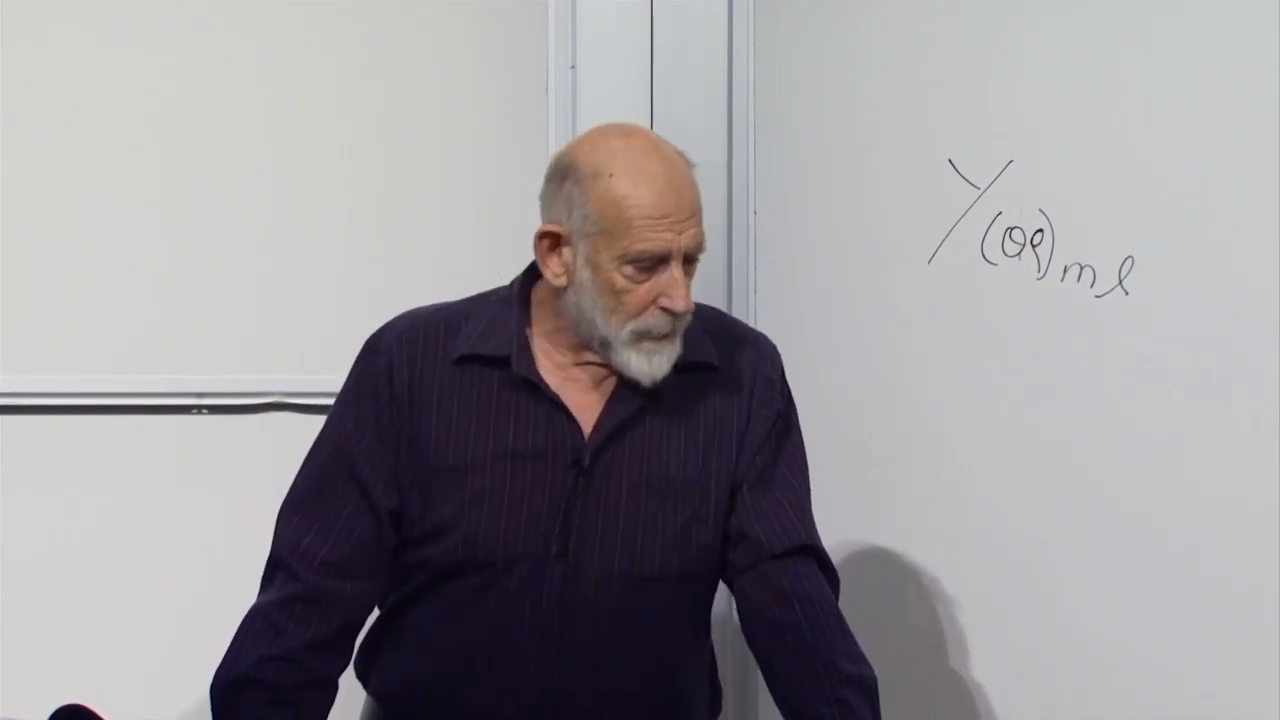
\includegraphics[width=0.9\linewidth]{lecture_03_frame_02.png}\caption{À moment cinétique classique fixé, le Hamiltonien radial comprend l’énergie cinétique radiale, le terme centrifuge \(L^2/(2mr^2)\) et le potentiel central \(V(r)\).}\lectureframe{00:47:15}\end{figure}

Le terme \(1/r^2\) constitue la barrière centrifuge. Il augmente à mesure que la particule s’approche de l’origine ; la force associée est donc dirigée vers l’extérieur. Pour les potentiels attractifs de type coulombien considérés ici, une trajectoire avec \(L\neq0\) contourne le centre au lieu de l’atteindre. Lorsque \(L=0\), la barrière disparaît.

Pour le potentiel coulombien attractif,
\begin{equation}
V(r)=-\frac{\kappa}{r},
\end{equation}
le terme centrifuge domine aux petites valeurs de \(r\), tandis que le terme coulombien décroît moins vite et domine aux grandes valeurs de \(r\). Pour \(L\neq0\), leur somme présente un minimum. Au minimum, le mouvement se fait à rayon constant et est donc circulaire. Au-dessus du minimum et en dessous du seuil d’échappement, le mouvement lié oscille entre un rayon minimal et un rayon maximal ; dans le problème coulombien, ces oscillations radiales correspondent aux oscillations d’une orbite elliptique.

\section{L’équation radiale réduite}

En mécanique quantique, la partie angulaire d’un état de moment cinétique orbital bien défini est une harmonique sphérique. Écrivons l’état séparé sous la forme
\begin{equation}
\Psi_{n_r\ell m}(r,\theta,\phi)
=\frac{u_{n_r\ell}(r)}{r}\,
Y_{\ell m}(\theta,\phi).
\end{equation}
L’opérateur angulaire \(L^2\) a pour valeur propre
\begin{equation}
L^2Y_{\ell m}
=\hbar^2\ell(\ell+1)Y_{\ell m}.
\end{equation}
Pour une paire fixée \(n_r,\ell\), abrégeons \(u_{n_r\ell}(r)\) en \(u(r)\). Il reste à résoudre pour la fonction radiale réduite l’équation
\begin{equation}
\begin{aligned}
&-\frac{\hbar^2}{2m}\frac{d^2u}{dr^2}
+\frac{\hbar^2\ell(\ell+1)}{2mr^2}u(r)\\
&\qquad+V(r)u(r)=E_{n_r\ell}\,u(r).
\end{aligned}
\end{equation}

\editorialnote{L’équation purement unidimensionnelle faisant intervenir la dérivée seconde s’écrit pour la fonction radiale réduite \(u=rR\). Ainsi, le \(\psi(r)\) dans l’équation affichée pendant le cours correspond à \(u(r)\), tandis que le facteur radial ordinaire dans \(\Psi=R(r)Y_{\ell m}\) est \(R=u/r\). Cette convention évite de traiter \(-i\hbar\,d/dr\) comme un opérateur autonome de quantité de mouvement radiale hermitien sur l’espace de Hilbert radial tridimensionnel.}

L’équation radiale réduite est représentée au tableau ci-dessous.\footnote{Image source : \texttt{\detokenize{lecture_03_frame_03.png}}, vidéo du cours à \(00{:}54{:}32\).}

\begin{figure}[htbp]\centering
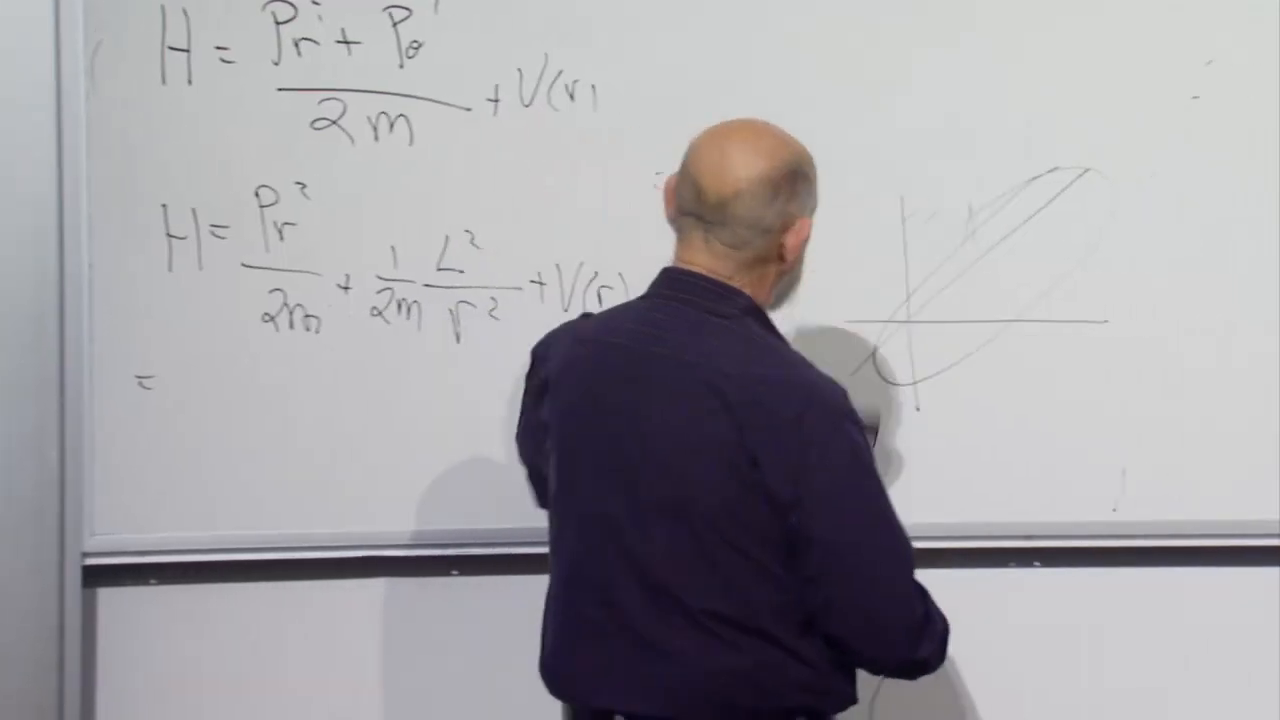
\includegraphics[width=0.9\linewidth]{lecture_03_frame_03.png}\caption{À \(\ell\) fixé, la fonction d’onde radiale réduite vérifie une équation de Schr\"odinger unidimensionnelle, avec un terme centrifuge proportionnel à \(\ell(\ell+1)/r^2\).}\lectureframe{00:54:32}\end{figure}

La structure angulaire tridimensionnelle est condensée dans le paramètre \(\ell\). Le nombre quantique magnétique \(m\) n’intervient pas dans l’équation radiale.

\begin{classroomqa}\lecturetimestamp{00:55:34}\audiencequestion{Pour une valeur donnée de \(\ell\), les \(2\ell+1\) états magnétiques ont-ils la même énergie ?}\lecturerresponse{Oui, à condition de fixer aussi l’état propre radial. Pour chaque valeur choisie de \(u_{n_r\ell}\), toutes les valeurs \(m=-\ell,\ldots,\ell\) ont la même énergie, car \(m\) n’intervient pas dans l’équation radiale. En général, des états propres radiaux différents associés à la même valeur de \(\ell\) ont des énergies différentes.}\end{classroomqa}

\begin{classroomqa}\lecturetimestamp{00:56:03}\audiencequestion{Pourquoi peut-on remplacer \(L^2\) par \(\hbar^2\ell(\ell+1)\), et quel est le lien entre \(\ell\) et les valeurs permises de \(m\) ?}\lecturerresponse{Le nombre \(\ell\) indexe un multiplet de moment cinétique et en est la plus grande valeur de \(m\). Tous les états de ce multiplet ont la même valeur propre de \(L^2\), soit \(\hbar^2\ell(\ell+1)\) ; c’est donc cette valeur propre que l’on introduit dans l’équation radiale.}\end{classroomqa}

Il n’est pas nécessaire de connaître les solutions explicites en fonctions spéciales pour l’argument présenté ici. Ce qui importe, c’est la façon dont les solutions s’organisent.

\section{Nœuds radiaux et niveaux d’énergie}

À \(\ell\) fixé, l’équation radiale réduite est un problème aux valeurs propres ordinaire à une dimension. Ses états liés se classent selon leur nombre de nœuds intérieurs. L’état radial le plus bas n’a aucun nœud intérieur, le suivant en a un, et celui d’après en a deux. Un plus grand nombre de nœuds signifie que la fonction d’onde varie plus rapidement ; une variation plus rapide implique une quantité de mouvement plus grande et donc une énergie cinétique plus élevée.

Chaque valeur de \(\ell\) définit un opérateur radial différent, car le terme centrifuge varie avec \(\ell\). Les valeurs \(\ell=0,1,2,\ldots\) donnent donc des suites radiales distinctes. Le terme centrifuge positif décale les niveaux vers le haut lorsque le moment cinétique augmente. Chaque valeur propre radiale à \(\ell\) fixé est associée à un multiplet magnétique de dimension
\begin{equation}
2\ell+1.
\end{equation}
Les niveaux \(\ell=0\) sont des singulets, les niveaux \(\ell=1\) des triplets et les niveaux \(\ell=2\) des quintuplets. Ce sont les dégénérescences imposées par la symétrie de rotation ; une symétrie supplémentaire peut aussi rendre dégénérés des états de valeurs différentes de \(\ell\).

Pour les potentiels de type atomique qui vérifient \(V(r)\to0\) aux grandes valeurs de \(r\), le seuil d’échappement est conventionnellement fixé à \(E=0\). Les états d’énergie négative forment le spectre discret des états liés. À \(E=0\) et au-delà, on trouve le continuum de diffusion. Cette affirmation dépend du comportement du potentiel aux grandes valeurs de \(r\) et ne s’applique pas à un potentiel central confinant.

\section{La dégénérescence particulière du potentiel coulombien}

Le potentiel coulombien non relativiste exact présente un alignement supplémentaire des niveaux. L’état radial le plus bas avec \(\ell=1\) a la même énergie que l’état \(\ell=0\) du premier niveau excité. L’état \(\ell=1\) suivant s’aligne sur l’état \(\ell=0\) du deuxième niveau excité, auquel se joint l’état \(\ell=2\) le plus bas. Le motif se poursuit dans les suites radiales et de moment cinétique orbital de plus en plus élevées.

\begin{classroomqa}\lecturetimestamp{01:09:57}\audiencequestion{Cette dégénérescence coulombienne supplémentaire révèle-t-elle une autre symétrie ?}\lecturerresponse{Oui. Elle correspond à une symétrie supplémentaire inhabituelle du potentiel coulombien exact. De faibles modifications du potentiel détruisent cet alignement ; sa dérivation ne sera pas abordée ici.}\end{classroomqa}

Les dégénérescences qui en résultent pour les couches orbitales sont
\begin{equation}
1,\qquad 4,\qquad 9,\qquad 16,\qquad \ldots
\end{equation}
avant la prise en compte du spin de l’électron.

\begin{classroomqa}\lecturetimestamp{01:11:46}\audiencequestion{Cette dégénérescence décrit-elle l’hydrogène, ou seulement le problème coulombien idéal ?}\lecturerresponse{L’hydrogène la vérifie à une très bonne approximation, mais pas exactement. Les corrections relativistes et la taille finie du noyau perturbent le motif coulombien idéal.}\end{classroomqa}

Un noyau ponctuel produit un potentiel exact en \(1/r\). Un noyau dont la charge est répartie dans un petit volume produit un potentiel légèrement différent lorsque l’électron pénètre dans ce volume ; même ce faible écart lève une partie de la dégénérescence particulière.

Le spin a également été omis. La prise en compte des deux états de spin de l’électron double les nombres d’états des couches :
\begin{equation}
2,\qquad 8,\qquad 18,\qquad 32,\qquad \ldots
\end{equation}
avant l’apparition des dédoublements supplémentaires dans un traitement atomique plus complet.

\section{Retour à l’équation cartésienne}

L’équation à l’origine du problème radial est l’équation de Schr\"odinger tridimensionnelle indépendante du temps :
\begin{equation}
\begin{aligned}
-\frac{\hbar^2}{2m}\nabla^2\Psi+V(r)\Psi&=E\Psi,\\
\nabla^2&=\frac{\partial^2}{\partial x^2}
+\frac{\partial^2}{\partial y^2}
+\frac{\partial^2}{\partial z^2},\\
r&=\sqrt{x^2+y^2+z^2}.
\end{aligned}
\end{equation}
Passons aux coordonnées radiales et angulaires et choisissons un état propre de \(L^2\).
En remplaçant \(L^2\) par \(\hbar^2\ell(\ell+1)\), on réduit alors l’équation aux dérivées partielles à l’équation radiale ordinaire obtenue plus haut.

\begin{classroomqa}\lecturetimestamp{01:16:42}\audiencequestion{Les écarts au spectre coulombien idéal pourraient-ils servir à déterminer la taille du noyau ?}\lecturerresponse{Pas avec cette comparaison simple. D’autres corrections, beaucoup plus importantes, doivent d’abord être prises en compte. La taille du noyau est mentionnée ici parce qu’elle fournit un exemple immédiat d’écart au potentiel coulombien ponctuel.}\end{classroomqa}

\begin{classroomqa}\lecturetimestamp{01:17:09}\audiencequestion{Quelle est la principale différence entre les termes de moment cinétique classique et quantique ?}\lecturerresponse{En mécanique classique, \(L^2\) est simplement le carré de la norme d’un vecteur conservé. Dans un multiplet orbital quantique, sa valeur propre est \(\hbar^2\ell(\ell+1)\), et non simplement \(\hbar^2\ell^2\). Le terme supplémentaire découle de la non-commutativité des composantes du moment cinétique.}\end{classroomqa}

\begin{classroomqa}\lecturetimestamp{01:17:58}\audiencequestion{Les fonctions d’onde des états liés ont-elles un support compact ?}\lecturerresponse{Non. Elles s’étendent à toute distance du centre. Pour les états liés atomiques considérés ici, elles décroissent exponentiellement à grande distance ; la probabilité devient donc négligeable, mais ne s’annule pas au-delà d’un rayon fini.}\end{classroomqa}

\begin{classroomqa}\lecturetimestamp{01:18:48}\audiencequestion{Lorsque \(\ell=0\) supprime le puits centrifuge, qu’advient-il du point stable ?}\lecturerresponse{Il n’y a plus de minimum résultant de la compétition entre la barrière centrifuge et l’attraction. Dans l’idéalisation d’un potentiel coulombien ponctuel, le mouvement classique se dirige vers le centre singulier. En mécanique quantique, l’état le plus bas ne peut avoir à la fois une position exactement définie au centre et une quantité de mouvement nulle ; sa fonction d’onde présente donc une extension spatiale finie.}\end{classroomqa}

\editorialnote{Pour un potentiel central régulier, une trajectoire classique de moment cinétique nul peut se poursuivre en traversant l’origine. En revanche, pour le potentiel coulombien ponctuel idéal, \(r=0\) est une singularité de collision, et la poursuite de la trajectoire classique nécessite une prescription supplémentaire.}

La réduction classique plaçait une orbite unique dans un plan, mais on ne peut pas procéder de la même manière pour une fonction d’onde quantique. Un état orbital quantique occupe l’espace tridimensionnel. L’opérateur angulaire complet est \(L^2=L_x^2+L_y^2+L_z^2\), et sa valeur propre conserve le résultat tridimensionnel \(\hbar^2\ell(\ell+1)\).

\begin{classroomqa}\lecturetimestamp{01:21:30}\audiencequestion{Comment le problème quantique peut-il rester tridimensionnel alors que l’orbite classique a été placée dans un plan ?}\lecturerresponse{Seule l’orbite classique a été placée dans un plan fixe en choisissant les coordonnées perpendiculaires à son vecteur moment cinétique conservé. Une fonction d’onde quantique occupe l’espace tridimensionnel. Les autres composantes du moment cinétique restent présentes dans \(L^2\), ce qui explique pourquoi l’équation radiale contient \(\ell(\ell+1)\) plutôt que le carré d’une seule composante.}\end{classroomqa}

\begin{classroomqa}\lecturetimestamp{01:22:54}\audiencequestion{Tout problème quantique admet-il des opérateurs d’élévation et d’abaissement ?}\lecturerresponse{Non. Ils apparaissent dans des cas particulièrement favorables. Le moment cinétique en est un, et l’oscillateur harmonique en est un autre. Le cas de l’oscillateur est particulièrement utile car le mouvement au voisinage d’un équilibre stable est très souvent approximativement harmonique, notamment les petites oscillations radiales près du minimum d’un potentiel effectif.}\end{classroomqa}

Le problème atomique est laissé de côté à ce stade, et l’oscillateur harmonique devient le prochain exemple de spectre déterminé par des opérateurs d’échelle.

\section{Petites oscillations et oscillateur harmonique}

Au voisinage d’un équilibre stable, un déplacement suffisamment petit produit souvent un mouvement harmonique. Le potentiel radial effectif pour un moment cinétique non nul en fournit un exemple : près du fond de son puits, le mouvement radial est approximativement harmonique.

Considérons un oscillateur unidimensionnel de masse unité. Soit \(x\) le déplacement par rapport à l’équilibre, et écrivons la constante de raideur \(k=\omega^2\). Le Hamiltonien classique est
\begin{equation}
H=\frac{p^2}{2}+\frac{\omega^2x^2}{2}.
\end{equation}
Les équations de Hamilton donnent
\begin{equation}
\dot{x}=\frac{\partial H}{\partial p}=p,
\qquad
\dot{p}=-\frac{\partial H}{\partial x}=-\omega^2x,
\end{equation}
et donc
\begin{equation}
\ddot{x}=-\omega^2x.
\end{equation}
Ainsi, \(\omega\) est la fréquence des oscillations classiques.

\section{Factorisation et énergie de point zéro}

En mécanique quantique,
\begin{equation}
[x,p]=i\hbar.
\end{equation}
Le Hamiltonien est une somme de carrés, ce qui suggère la factorisation
\begin{align}
\frac{1}{2}(p+i\omega x)(p-i\omega x)
&=\frac{1}{2}\left(p^2+\omega^2x^2+i\omega[x,p]\right) \\
&=\frac{1}{2}\left(p^2+\omega^2x^2-\hbar\omega\right).
\end{align}
On obtient donc
\begin{equation}
H=\frac{1}{2}(p+i\omega x)(p-i\omega x)
+\frac{1}{2}\hbar\omega.
\end{equation}
Le terme additif \(\hbar\omega/2\) est l’énergie de point zéro.

Classiquement, l’énergie minimale serait atteinte en \(x=p=0\). En mécanique quantique, aucun état ne peut avoir simultanément une position et une quantité de mouvement exactement fixées à zéro. De plus, les deux termes \(p^2/2\) et \(\omega^2x^2/2\) sont positifs et ne peuvent pas se compenser. Une énergie de l’état fondamental non nulle est donc inévitable.

Pour le calcul avec les opérateurs d’échelle, on peut provisoirement mettre de côté la constante additive commune et la rétablir à la fin.

\begin{classroomqa}\lecturetimestamp{01:36:10}\audiencequestion{Le signe positif du terme d’énergie de point zéro nous apprend-il quelque chose de plus ?}\lecturerresponse{Le Hamiltonien de l’oscillateur est un opérateur positif : c’est une somme de carrés positifs, et son énergie ne peut donc pas être négative.}\end{classroomqa}

\section{L’échelle de l’oscillateur}

Introduisons les opérateurs sans dimension\footnote{Autour de \(01{:}37\)--\(01{:}42\), le calcul prend \(\hbar=1\). Le facteur \(\hbar\) est rétabli dans ces définitions normalisées afin que \(A_\pm\) soient sans dimension et que leur commutateur soit égal à l’unité.}
\begin{equation}
A_+=\frac{p+i\omega x}{\sqrt{2\hbar\omega}},
\qquad
A_-=\frac{p-i\omega x}{\sqrt{2\hbar\omega}}.
\end{equation}
Ils sont conjugués hermitiens :
\begin{equation}
A_+^\dagger=A_-.
\end{equation}
Leur commutateur est
\begin{align}
[A_-,A_+]
&=\frac{1}{2\hbar\omega}
\left([p,i\omega x]+[-i\omega x,p]\right) \\
&=1.
\end{align}

Définissons
\begin{equation}
N=A_+A_-.
\end{equation}
Le Hamiltonien s’écrit alors
\begin{equation}
H=\hbar\omega\left(N+\frac{1}{2}\right).
\end{equation}
La détermination du spectre d’énergie se réduit donc à celle des valeurs propres de \(N\).

Supposons que
\begin{equation}
N|n\rangle=n|n\rangle.
\end{equation}
Les commutateurs avec \(N\) sont\footnote{Les étapes intermédiaires à \(01{:}45{:}37\)--\(01{:}48{:}10\) sont reconstituées directement à partir des relations énoncées \(N=A_+A_-\) et \([A_-,A_+]=1\).}
\begin{align}
[N,A_+]
&=A_+[A_-,A_+]=A_+, \\
[N,A_-]
&=[A_+,A_-]A_-=-A_-.
\end{align}
Il s’ensuit que
\begin{align}
N\bigl(A_+|n\rangle\bigr)
&=(n+1)A_+|n\rangle, \\
N\bigl(A_-|n\rangle\bigr)
&=(n-1)A_-|n\rangle.
\end{align}
Ainsi, \(A_+\) augmente d’une unité une valeur propre de \(N\), et \(A_-\) la diminue d’une unité, chaque fois que le vecteur obtenu est non nul.

L’opérateur \(N\) est positif ou nul :
\begin{equation}
\langle\psi|N|\psi\rangle
=\langle\psi|A_+A_-|\psi\rangle
=\|A_-|\psi\rangle\|^2
\geq0.
\end{equation}
Le processus d’abaissement ne peut donc pas se poursuivre jusqu’à des valeurs propres négatives. Il doit s’arrêter à un état inférieur \(|b\rangle\) :
\begin{equation}
A_-|b\rangle=0.
\end{equation}

Pour les états propres normalisés, les normes fixent les coefficients de l’échelle :
\begin{align}
\|A_-|n\rangle\|^2
&=\langle n|A_+A_-|n\rangle=n, \\
\|A_+|n\rangle\|^2
&=\langle n|A_-A_+|n\rangle=n+1.
\end{align}
On peut donc choisir les phases de sorte que
\begin{equation}
A_-|n\rangle=\sqrt{n}\,|n-1\rangle,
\qquad
A_+|n\rangle=\sqrt{n+1}\,|n+1\rangle.
\end{equation}

\begin{classroomqa}\lecturetimestamp{01:52:42}\audiencequestion{Si \(A_-\) abaisse un état et que \(A_+\) le relève ensuite, comment \(A_+A_-\) donne-t-il la valeur propre \(n\) ?}\lecturerresponse{L’action des opérateurs d’échelle comprend des facteurs de normalisation. L’action de \(A_-\) apporte le facteur \(\sqrt n\), puis celle de \(A_+\) sur l’état obtenu apporte un autre facteur \(\sqrt n\). Leur produit vaut \(n\).}\end{classroomqa}

En effet,
\begin{equation}
A_+A_-|n\rangle
=\sqrt n\,A_+|n-1\rangle
=n|n\rangle.
\end{equation}

\begin{classroomqa}\lecturetimestamp{01:55:52}\audiencequestion{La plus petite valeur propre de \(N\) doit-elle être nulle, ou pourrait-elle être positive ?}\lecturerresponse{Elle doit être nulle, et le spectre de \(N\) est constitué des entiers non négatifs. La démonstration de cette valeur à l’extrémité de l’échelle n’a pas encore été donnée.}\end{classroomqa}

\editorialnote{Soit \(|b\rangle\) un état inférieur. Puisque l’abaissement doit s’arrêter, \(A_-|b\rangle=0\). Il s’ensuit immédiatement que \(N|b\rangle=A_+A_-|b\rangle=0\) ; la valeur propre la plus basse de \(N\) est donc nulle.}

À partir de cet état inférieur, l’application de \(A_+\) donne
\begin{equation}
n=0,1,2,\ldots.
\end{equation}
En rétablissant le terme additif d’énergie de point zéro, les énergies de l’oscillateur sont
\begin{equation}
E_n=\hbar\omega\left(n+\frac{1}{2}\right),
\qquad n=0,1,2,\ldots.
\end{equation}

L’algèbre de l’oscillateur sera développée davantage et utilisée pour résoudre d’autres problèmes quantiques.

\chapter{Fonctions d’onde de l’oscillateur, spin un demi et échange de particules}

\section{Des oscillateurs partout}

Tout système possédant un équilibre stable peut osciller lorsqu’on l’en écarte. Il peut avoir une seule fréquence ou plusieurs. Une corde de violon, par exemple, possède un mode fondamental et des harmoniques supérieures. La pincer excite une certaine combinaison de ces modes.

Les exemples les plus importants ici sont les champs. La configuration d’équilibre du champ électromagnétique est le vide : pas de champ électrique, pas de champ magnétique et pas d’oscillation électromagnétique. Si l’on introduit un rayonnement dans une cavité ou un guide d’ondes, le champ peut osciller selon ses modes permis, chacun ayant sa propre fréquence. Dans la théorie quantique, ces modes décrivent des ensembles de photons.

La même idée s’applique à un cristal. Il est trompeur de se représenter chaque atome comme un oscillateur indépendant. Les atomes exercent des forces les uns sur les autres, si bien que le déplacement d’un atome affecte ses voisins et qu’une onde se propage dans le cristal. Les modes normaux de ce mouvement couplé sont des oscillateurs harmoniques, et leurs quanta sont appelés phonons. Photons et phonons sont des objets physiques différents, mais tous deux ramènent à la même algèbre de l’oscillateur.

\section{L’algèbre de l’oscillateur}

Pour étudier l’oscillateur, posons la masse et la constante de Planck réduite égales à un :
\[
m=1,\qquad \hbar=1.
\]
Le Hamiltonien est
\begin{equation}
H=\frac{p^{2}}{2}+\frac{\omega^{2}x^{2}}{2}.
\end{equation}
Le paramètre \(\omega\) fixe la courbure du potentiel et correspond aussi à la fréquence d’oscillation.

Définissons les opérateurs de montée et de descente par
\begin{equation}
A_{\pm}=\frac{p\pm i\omega x}{\sqrt{2\omega}}.
\end{equation}
La normalisation est choisie de sorte que
\begin{equation}
[A_{-},A_{+}]=1.
\end{equation}
L’opérateur nombre est
\begin{equation}
N=A_{+}A_{-}.
\end{equation}
Ensemble, ces équations impliquent que \(A_{+}\) augmente d’une unité une valeur propre de \(N\) et que \(A_{-}\) la diminue d’une unité. Le spectre qui en résulte est
\begin{equation}
n=0,1,2,3,\ldots .
\end{equation}

Le produit des deux opérateurs d’échelle fait aussi apparaître la correction quantique à l’énergie classique :
\begin{align}
N
&=\frac{1}{2\omega}(p+i\omega x)(p-i\omega x)\\
&=\frac{1}{2\omega}\left(p^{2}+\omega^{2}x^{2}
 +i\omega[x,p]\right)\\
&=\frac{1}{2\omega}\left(p^{2}+\omega^{2}x^{2}-\omega\right),
\end{align}
où \([x,p]=i\). Par conséquent,
\begin{equation}
H=\omega\left(N+\frac12\right).
\end{equation}
Si la constante additive n’a pas d’importance pour le problème, il est commode d’utiliser le Hamiltonien décalé
\begin{equation}
H_{\mathrm{shifted}}=H-\frac{\omega}{2}=\omega N.
\end{equation}
Le terme \(\omega/2\) est l’énergie de point zéro, ou énergie de l’état fondamental, de l’oscillateur. Pour un mode de champ, le terme analogue est appelé énergie du vide. Il reflète le principe d’incertitude : aucun état ne peut avoir à la fois \(x\) et \(p\) exactement égaux à zéro, si bien que les deux termes quadratiques positifs dans \(H\) ne peuvent pas avoir tous deux une valeur moyenne nulle.

\begin{classroomqa}
\lecturetimestamp{00:09:46}
\audiencequestion{Pourquoi zéro fait-il partie du spectre de l’opérateur nombre ?}
\lecturerresponse{On peut le démontrer explicitement en construisant la fonction d’onde de l’état fondamental. Cette construction fera apparaître un état tel que \(N=0\).}
\end{classroomqa}

Pour commencer cette construction, remplaçons les vecteurs d’état par des fonctions d’onde de position. Les états propres de l’énergie deviennent
\[
\psi_{0}(x),\ \psi_{1}(x),\ \psi_{2}(x),\ldots,
\]
et les opérateurs fondamentaux agissent comme suit :
\begin{equation}
X\longmapsto x,\qquad
P\longmapsto -i\frac{d}{dx}.
\end{equation}
En rétablissant \(\hbar\), le second remplacement serait
\(P\mapsto-i\hbar\,d/dx\).

Avant de résoudre l’équation pour \(\psi_{0}\), on peut répondre plus rapidement à la question par un raisonnement abstrait. Sur l’échelle discrète des états propres normalisables de l’oscillateur, \(N=A_{+}A_{-}\) est non négatif ; des abaissements répétés par unités ne peuvent donc pas se poursuivre indéfiniment. À l’extrémité---dont on construira plus bas la fonction d’onde normalisable---il doit exister un état, noté \(\lvert0\rangle\), tel que
\begin{equation}
A_{-}\lvert0\rangle=\mathbf 0.
\end{equation}
Sinon, \(A_{-}\lvert0\rangle\) serait un autre état, situé une unité plus bas. Il s’ensuit immédiatement que
\begin{equation}
N\lvert0\rangle
=A_{+}A_{-}\lvert0\rangle
=\mathbf 0
=0\,\lvert0\rangle.
\end{equation}
L’état le plus bas a donc pour valeur propre de nombre zéro.

\begin{classroomqa}
\lecturetimestamp{00:14:57}
\audiencequestion{Si la valeur propre est zéro, le membre de droite ne devrait-il pas contenir un vecteur propre nul ?}
\lecturerresponse{Le ket \(\lvert0\rangle\) est un vecteur normalisé non nul dont l’étiquette est zéro. Dans \(N\lvert0\rangle=0\,\lvert0\rangle\), le membre de droite est le vecteur nul. Le ket de l’état fondamental et le vecteur nul sont des objets différents.}
\end{classroomqa}

\section{L’équation de Schr\"odinger et les solutions physiques}

Revenons maintenant à la représentation de position. L’équation de Schr\"odinger indépendante du temps est
\begin{equation}
\left[
-\frac12\frac{d^{2}}{dx^{2}}
+\frac12\omega^{2}x^{2}
\right]\psi(x)=E\psi(x).
\end{equation}
En tant qu’équation différentielle du second ordre, elle possède des solutions formelles pour des valeurs arbitraires de \(E\). La plupart de ces solutions formelles ne correspondent pas à des états physiques de l’oscillateur. Elles croissent exponentiellement lorsque \(\lvert x\rvert\) devient grand, si bien que leur norme diverge.

Pour un état lié, la fonction d’onde doit être de carré intégrable :
\begin{equation}
\int_{-\infty}^{\infty}\psi^{*}(x)\psi(x)\,dx<\infty.
\end{equation}
On peut alors la normaliser de sorte que l’intégrale soit égale à un. Seules certaines valeurs particulières de l’énergie donnent de telles solutions. À cet égard, les états de position et de quantité de mouvement sur une droite infinie font exception, mais les solutions de l’oscillateur qui croissent exponentiellement sont tout simplement exclues de l’espace des états.

\section{L’état fondamental gaussien}

On peut résoudre l’équation du second ordre, mais l’algèbre des opérateurs d’échelle donne une équation du premier ordre plus simple :
\begin{equation}
A_{-}\psi_{0}(x)=0.
\end{equation}
Le facteur global dans \(A_{-}\) n’a pas d’importance lorsque le membre de droite est nul ; cette équation équivaut donc à
\begin{equation}
(p-i\omega x)\psi_{0}(x)=0.
\end{equation}
En utilisant \(p=-i\,d/dx\), on obtient
\begin{equation}
\left(\frac{d}{dx}+\omega x\right)\psi_{0}(x)=0.
\end{equation}

\begin{classroomqa}
\lecturetimestamp{00:22:32}
\audiencequestion{Peut-on résoudre cette équation par séparation des variables ?}
\lecturerresponse{Il n’y a qu’une variable indépendante ; il n’y a donc pas deux variables à séparer. Écrite sous la forme \(\psi_{0}'/\psi_{0}=-\omega x\), l’équation ressemble à une dérivée logarithmique. Cela suggère d’écrire la fonction d’onde sous forme exponentielle.}
\end{classroomqa}

Une méthode utile consiste à poser
\begin{equation}
\psi_{0}(x)=e^{f(x)}.
\end{equation}
Alors
\[
\psi_{0}'(x)=f'(x)e^{f(x)},
\]
et le facteur exponentiel commun se simplifie. L’équation se réduit à
\begin{equation}
\frac{df}{dx}+\omega x=0.
\end{equation}

\begin{classroomqa}
\lecturetimestamp{00:26:28}
\audiencequestion{Ne devrait-il pas y avoir un signe moins dans \(f(x)\) ?}
\lecturerresponse{Oui. Puisque \(df/dx=-\omega x\), l’intégration donne un terme quadratique négatif.}
\end{classroomqa}

On a donc
\begin{equation}
f(x)=-\frac12\omega x^{2}+C,
\end{equation}
et
\begin{equation}
\psi_{0}(x)\propto e^{-\omega x^{2}/2}.
\end{equation}
La constante multiplicative de normalisation n’est pas précisée. L’essentiel est la forme gaussienne : la fonction est lisse, concentrée près de l’origine et décroît rapidement lorsque \(\lvert x\rvert\) devient grand. Elle est manifestement de carré intégrable.

Il n’est pas nécessaire de réinjecter la réponse dans l’équation du second ordre pour trouver son énergie. L’algèbre donne déjà
\begin{equation}
E_{0}=\frac{\omega}{2}.
\end{equation}

\section{États excités, nœuds et mouvement classique}

Le premier état excité s’obtient en appliquant l’opérateur de montée à l’état fondamental :
\begin{equation}
\psi_{1}(x)\propto A_{+}\psi_{0}(x)
\propto(p+i\omega x)e^{-\omega x^{2}/2}.
\end{equation}
L’équation de l’état fondamental indique que
\[
p\psi_{0}=i\omega x\,\psi_{0}.
\]
Le changement de signe dans l’opérateur d’échelle transforme la soustraction en addition :
\begin{equation}
(p+i\omega x)\psi_{0}
=2i\omega x\,\psi_{0}.
\end{equation}
À une constante globale près,
\begin{equation}
\psi_{1}(x)\propto x\,e^{-\omega x^{2}/2}.
\end{equation}

Cette fonction d’onde est impaire :
\begin{equation}
\psi_{1}(-x)=-\psi_{1}(x).
\end{equation}
Sa densité de probabilité est paire, mais elle possède un nœud à l’origine,
\begin{equation}
\lvert\psi_{1}(0)\rvert^{2}=0.
\end{equation}
La densité de probabilité du premier état excité possède donc un nœud en \(x=0\).

Des applications répétées de \(A_{+}\) donnent des polynômes de degré croissant multipliant la même enveloppe gaussienne.\footnote{Le cours indique les facteurs polynomiaux de degré supérieur, le nœud supplémentaire à chaque étape et l’alternance de parité de \(00{:}34{:}25\) à \(00{:}35{:}49\). La forme produit d’une gaussienne par un polynôme est confirmée par la discussion des fonctions propres de l’oscillateur dans l’ouvrage de Leonard Susskind et Art Friedman, \emph{Quantum Mechanics: The Theoretical Minimum} (2014).}À un facteur de normalisation près,
\begin{equation}
\psi_{n}(x)=P_{n}(x)e^{-\omega x^{2}/2}.
\end{equation}
La parité alterne entre paire et impaire, et chaque étape ajoute un nœud. Lorsque \(n\) augmente, la fonction d’onde s’étend plus loin de l’origine et ses oscillations deviennent plus rapides.

Ces deux caractéristiques ont des significations physiques directes. Une fonction d’onde qui s’étend plus loin de l’origine correspond à une énergie potentielle plus élevée, car le potentiel croît comme \(x^{2}\). Des oscillations rapides dans l’espace des positions signalent une quantité de mouvement plus grande. Un oscillateur fortement excité a tendance à s’éloigner davantage du centre ; lorsqu’il traverse la région centrale, sa quantité de mouvement est plus grande et sa fonction d’onde y oscille plus rapidement.

\begin{classroomqa}
\lecturetimestamp{00:37:18}
\audiencequestion{L’oscillateur harmonique cesse-t-il de se rapprocher du comportement classique lorsque \(n\) devient grand ?}
\lecturerresponse{Le mouvement classique n’est pas représenté par un seul état propre stationnaire de l’énergie. Il apparaît dans un paquet d’ondes qui contient plusieurs niveaux d’énergie. Une gaussienne déplacée, par exemple, évolue en oscillant comme un oscillateur classique, et l’incertitude relative diminue à mesure que l’amplitude de l’oscillation augmente.}
\end{classroomqa}

Partons de la gaussienne de l’état fondamental et déplaçons-la par rapport à l’origine. Le paquet ainsi déplacé n’est plus un état propre de l’énergie ; c’est une superposition de nombreux états propres. Selon l’équation de Schr\"odinger dépendante du temps, ses composantes acquièrent des phases différentes. Le paquet oscille d’un côté à l’autre du potentiel, présentant de rapides variations de phase près du centre et redevenant lisse près d’un point de retournement. Plus l’excursion est grande devant la largeur du paquet, plus le mouvement paraît classique.

\begin{classroomqa}
\lecturetimestamp{00:39:29}
\audiencequestion{La fonction d’onde du deuxième état excité devrait-elle s’annuler à l’origine ?}
\lecturerresponse{Non. Son facteur polynomial n’est pas simplement \(x^{2}\) ; il contient aussi un terme constant, de sorte que la fonction d’onde n’a pas nécessairement à s’annuler en \(x=0\).}
\end{classroomqa}

Le raisonnement par opérateurs d’échelle suppose aussi que \(A_{+}\) et \(A_{-}\) sont adjoints l’un de l’autre sur le domaine des fonctions de l’oscillateur de carré intégrable, avec le comportement aux limites requis pour la relation d’adjonction. Les solutions formelles qui croissent exponentiellement n’appartiennent pas à ce domaine.

\begin{classroomqa}
\lecturetimestamp{00:40:45}
\audiencequestion{Existe-t-il un moyen général de reconnaître les Hamiltoniens que l’on peut résoudre par ces méthodes algébriques ?}
\lecturerresponse{Il n’existe pas de règle générale de ce type. Les exemples exactement solubles sont rares. L’oscillateur harmonique et l’atome d’hydrogène idéal non relativiste sont des cas heureux où les méthodes algébriques fonctionnent.}
\end{classroomqa}

\section{Le spin un demi comme moment cinétique}

Le spin est un moment cinétique porté par une particule indépendamment de son mouvement orbital autour de son centre de masse. Une particule au repos n’a pas de moment cinétique orbital \(\mathbf R\times\mathbf P\), mais elle peut tout de même avoir un spin. On peut essayer de se représenter un minuscule objet en rotation, ou traiter le spin comme une propriété quantique intrinsèque. L’affirmation décisive est mathématique : ses composantes se transforment sous les rotations spatiales et obéissent aux relations de commutation du moment cinétique.

Rétablissons \(\hbar\) à partir d’ici. Les composantes du moment cinétique vérifient
\begin{equation}
[L_{z},L_{x}]=i\hbar L_{y},
\end{equation}
les deux autres relations s’obtenant par permutation cyclique. Les matrices de Pauli sans dimension sont
\begin{equation}
\begin{aligned}
\sigma_{z}&=
\begin{pmatrix}
1&0\\
0&-1
\end{pmatrix},\\[0.4em]
\sigma_{x}&=
\begin{pmatrix}
0&1\\
1&0
\end{pmatrix},\\[0.4em]
\sigma_{y}&=
\begin{pmatrix}
0&-i\\
i&0
\end{pmatrix}.
\end{aligned}
\end{equation}
Dans cette base, \(\sigma_{z}\) est diagonale. Ses valeurs propres sont \(+1\) et
\(-1\).

\begin{classroomqa}
\lecturetimestamp{00:47:35}
\audiencequestion{Y a-t-il un signe moins dans \(\sigma_x\) ?}
\lecturerresponse{Non. Les deux éléments hors diagonale de \(\sigma_x\) sont positifs.}
\end{classroomqa}

Le calcul au tableau à \(00{:}49{:}35\) commence le produit terme à terme. En terminant les produits, on obtient
\begin{align}
\sigma_{z}\sigma_{x}
&=
\begin{pmatrix}
0&1\\
-1&0
\end{pmatrix}
=i\sigma_{y},\\
\sigma_{x}\sigma_{z}
&=
\begin{pmatrix}
0&-1\\
1&0
\end{pmatrix}
=-i\sigma_{y}.
\end{align}
Il s’ensuit que
\begin{equation}
[\sigma_{z},\sigma_{x}]=2i\sigma_{y}.
\end{equation}
On élimine le facteur deux supplémentaire en définissant les opérateurs de spin physiques comme suit :\footnote{Le calcul au tableau omet \(\hbar\). Il est rétabli ici afin que \(S_i\) ait les unités d’un moment cinétique.}
\begin{equation}
S_{i}=\frac{\hbar}{2}\sigma_{i}.
\end{equation}
On a alors
\begin{equation}
[S_{z},S_{x}]=i\hbar S_{y},
\end{equation}
et de même pour les permutations cycliques. La moitié des matrices de Pauli, avec le facteur \(\hbar\) rétabli, forme donc un système de moment cinétique.

En posant \(\hbar=1\), on obtient la forme présentée ci-dessous.\footnote{La séquence source est \texttt{lecture\_04\_frame\_02.png}.}
\begin{figure}[htbp]
\centering
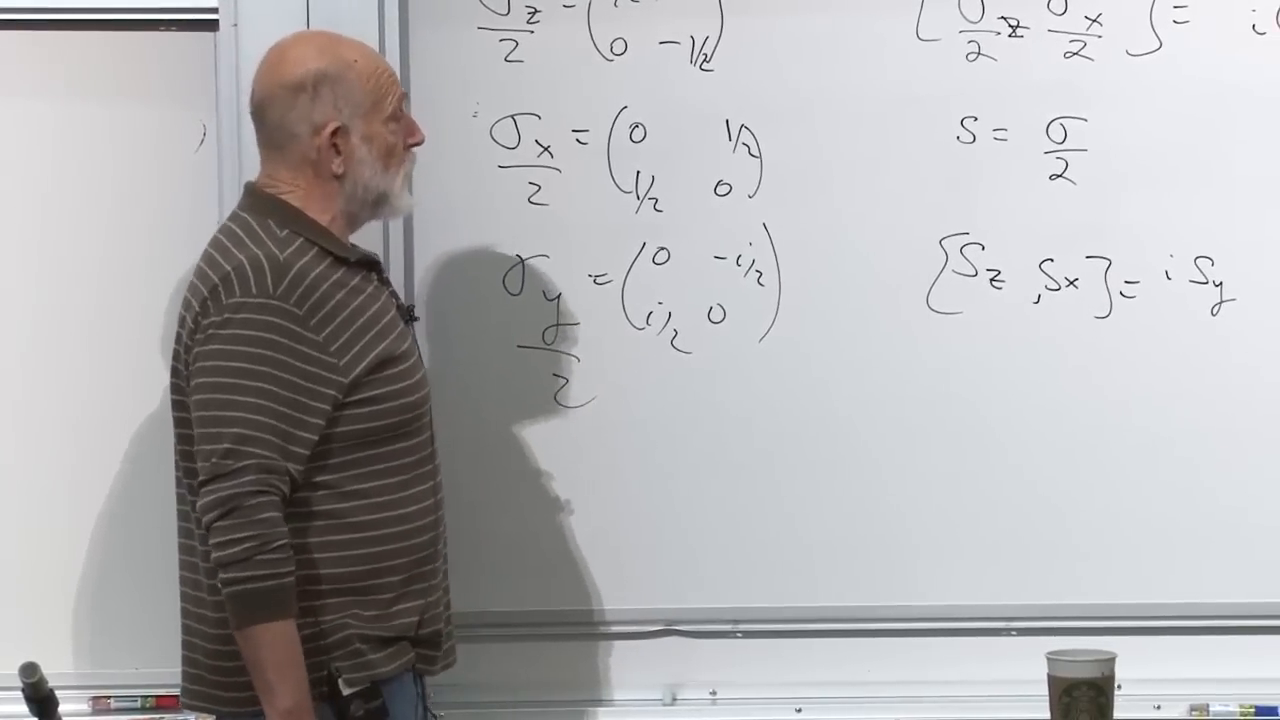
\includegraphics[width=0.9\linewidth]{lecture_04_frame_02.png}
\caption{En unités où \(\hbar=1\), la moitié des matrices de Pauli correspond aux opérateurs de moment cinétique de spin un demi et vérifie \([S_z,S_x]=iS_y\).}
\lectureframe{00:55:41}
\end{figure}

Les deux équations aux valeurs propres de \(S_z\) sont
\begin{equation}
S_z\lvert\pm\rangle
=\pm\frac{\hbar}{2}\lvert\pm\rangle.
\end{equation}
De manière équivalente, le nombre quantique magnétique sans dimension est
\begin{equation}
m_{s}=\pm\frac12,
\qquad
S_{z}\lvert m_{s}\rangle
=m_{s}\hbar\,\lvert m_{s}\rangle.
\end{equation}
Les opérateurs de montée et de descente du moment cinétique décalent \(m\) par pas entiers, mais cela n’implique pas que chaque échelle passe par zéro. Les multiplets de spin entier contiennent des valeurs entières de \(m\), tandis que ceux de spin demi-entier contiennent des valeurs demi-entières. Pour le spin un demi, l’échelle ne comporte que les deux états \(m_s=+1/2\) et \(m_s=-1/2\).

Ces deux états forment le doublet de spin un demi. Les électrons, les muons, les neutrinos et les quarks font partie des particules décrites par de tels multiplets de spin demi-entier.

\section{Moment cinétique orbital et spin}

Il existe maintenant deux types de moment cinétique. Le moment cinétique orbital décrit le mouvement par rapport à une origine,
\begin{equation}
\mathbf L=\mathbf R\times\mathbf P,
\end{equation}
tandis que \(\mathbf S\) est le spin intrinsèque. Leur somme vectorielle est le moment cinétique total,
\begin{equation}
\mathbf J=\mathbf L+\mathbf S.
\end{equation}

\begin{classroomqa}
\lecturetimestamp{00:56:49}
\audiencequestion{Si un système a un moment cinétique total \(\mathbf J\), comment détermine-t-on son spin \(\mathbf S\) ?}
\lecturerresponse{Les nombres quantiques de spin et de moment cinétique orbital sont normalement fournis séparément. Si \(L=0\), tout le moment cinétique est du spin. Sinon, il faut les règles quantiques d’addition des moments cinétiques, qui seront présentées plus tard.}
\end{classroomqa}

Les règles d’addition s’appliquent aussi bien à la somme du moment cinétique orbital et du spin qu’à deux spins ou à deux moments cinétiques orbitaux. Le système composé possède ses propres valeurs permises du moment cinétique total, mais ces règles ne sont pas encore nécessaires.

\begin{classroomqa}
\lecturetimestamp{00:58:18}
\audiencequestion{Quelles observations expérimentales ont conduit à introduire le spin ?}
\lecturerresponse{La spectroscopie en a fourni des indices, mais le tableau périodique donne une motivation particulièrement claire : sa structure en couches exige que les électrons possèdent une propriété supplémentaire à deux valeurs.}
\end{classroomqa}

\section{Dégénérescence hydrogénoïde et dénombrement des couches}

Pour le moment cinétique orbital, l’équation aux valeurs propres de \(L^{2}\) est
\begin{equation}
L^{2}\lvert\ell,m\rangle
=\hbar^{2}\ell(\ell+1)\lvert\ell,m\rangle,
\end{equation}
et une valeur fixée de \(\ell\) possède
\begin{equation}
2\ell+1
\end{equation}
états magnétiques, correspondant à \(m=-\ell,-\ell+1,\ldots,\ell\).

Le problème coulombien idéal non relativiste présente une dégénérescence supplémentaire. Les énergies des états liés sont négatives et tendent vers zéro par valeurs négatives, mais seul l’alignement des niveaux importe ici pour le dénombrement. Le premier niveau \(\ell=1\) est aligné sur le niveau \(\ell=0\) suivant ; le premier niveau \(\ell=2\) rejoint la couche principale suivante, et le motif se poursuit.\footnote{\texttt{lecture\_04\_frame\_03.png}, \(01{:}02{:}01\) ; l’alignement complet des couches principales est énoncé de \(01{:}02{:}33\) à \(01{:}04{:}10\).}

\begin{figure}[htbp]
\centering
\begin{tikzpicture}[x=1.55cm,y=1.0cm]
\draw[->] (-0.65,0) -- (-0.65,4.35);
\draw[->] (-0.85,0) -- (4.75,0);
\node at (-0.95,4.08) {\(E\)};
\node at (4.55,-0.28) {\(\ell\)};
\node at (0,-0.30) {\(0\)};
\node at (2,-0.30) {\(1\)};
\node at (4,-0.30) {\(2\)};

\draw (-0.20,0.75) -- (0.20,0.75);

\draw (-0.20,2.00) -- (0.20,2.00);
\foreach \dx in {-0.18,0,0.18}
  \draw (2+\dx-0.06,2.00) -- (2+\dx+0.06,2.00);

\draw (-0.20,3.15) -- (0.20,3.15);
\foreach \dx in {-0.18,0,0.18}
  \draw (2+\dx-0.06,3.15) -- (2+\dx+0.06,3.15);
\foreach \dx in {-0.32,-0.16,0,0.16,0.32}
  \draw (4+\dx-0.05,3.15) -- (4+\dx+0.05,3.15);

\node[anchor=west] at (0.35,0.75) {\(n=1\)};
\node[anchor=west] at (2.35,2.00) {\(n=2\)};
\node[anchor=west] at (4.40,3.15) {\(n=3\)};
\end{tikzpicture}
\caption{Les trois premières couches coulombiennes idéales regroupent des multiplets orbitaux de même énergie principale : un état dans la première couche, \(1+3\) dans la deuxième et \(1+3+5\) dans la troisième.}
\lectureframe{01:02:01}
\end{figure}

Dans la couche principale \(n\), les valeurs orbitales permises sont\footnote{Cette plage compacte de valeurs de \(\ell\) et la somme ci-dessous reconstituent les alignements de niveaux et les nombres d’états \(1,4,9,16,\ldots\) indiqués de \(01{:}02{:}33\) à \(01{:}04{:}10\). Le début du diagramme de spectre apparaît dans \texttt{lecture\_04\_frame\_03.png} à \(01{:}02{:}01\).}
\[
\ell=0,1,\ldots,n-1.
\]
Le nombre d’états spatiaux est donc
\begin{equation}
\sum_{\ell=0}^{n-1}(2\ell+1)=n^{2},
\end{equation}
ce qui donne la suite
\begin{equation}
1,\ 4,\ 9,\ 16,\ldots .
\end{equation}
Ce dénombrement ne porte que sur les états spatiaux. Chaque état spatial admet deux valeurs de spin ; les nombres totaux correspondants dans ce modèle idéal sont donc
\begin{equation}
2,\ 8,\ 18,\ 32,\ldots=2n^{2}.
\end{equation}

\section{Exclusion et propriété électronique à deux valeurs}

Commençons par l’hélium dans l’approximation des électrons indépendants. Son noyau porte une charge protonique double, ce qui redimensionne les niveaux hydrogénoïdes et attire les électrons vers le noyau. En négligeant pour l’instant les interactions électron--électron, deux électrons peuvent occuper la plus basse orbitale spatiale, ce qui donne une première approximation raisonnable de l’état fondamental de l’hélium.

Pourquoi ne pas y placer aussi un troisième électron ? Cela abaisserait son énergie orbitale, mais cela ne se produit pas. La restriction est le principe d’exclusion de Pauli : deux électrons ne peuvent occuper le même état complet à une particule. Il serait trompeur d’y voir une force répulsive ordinaire. Il s’agit d’une restriction sur les états quantiques permis.

Une contradiction apparente se présente. Les deux électrons de l’hélium occupent bien la même orbitale spatiale. La résolution est qu’un état électronique complet comprend davantage que la fonction d’onde orbitale. Il comporte aussi un degré de liberté à deux valeurs. Appelons-les haut et bas. Un électron dans l’orbitale la plus basse peut avoir un spin haut et l’autre un spin bas ; leurs états spatiaux sont identiques, mais leurs états quantiques complets diffèrent.

À ce stade, le dénombrement avance jusqu’au lithium, puis revient en arrière. Ce retour met en évidence pourquoi l’exclusion et le spin sont tous deux nécessaires. Imaginons une règle d’exclusion sans spin. Un seul électron pourrait occuper l’état spatial le plus bas. Un deuxième devrait entrer dans l’un des quatre états spatiaux de la couche principale suivante, ce qui donnerait plusieurs possibilités, alors que l’état fondamental observé de l’hélium est unique. Cette version sans spin du principe d’exclusion est erronée.

Rétablissons les deux valeurs de spin. Deux électrons remplissent l’orbitale la plus basse avec des spins opposés. Un troisième électron, comme dans le lithium neutre, doit entrer dans la couche principale suivante. Cette couche compte un état spatial \(\ell=0\) et trois états spatiaux \(\ell=1\). Avant de tenir compte du spin, il y a quatre possibilités.

\begin{classroomqa}
\lecturetimestamp{01:14:58}
\audiencequestion{Comment les états \(s\) et \(p\) donnent-ils huit possibilités dans la première couche excitée ?}
\lecturerresponse{Il y a un état spatial avec \(\ell=0\) et trois avec \(\ell=1\), soit quatre états spatiaux. Chacun admet deux valeurs de spin, donc le total est \(2(1+3)=8\).}
\end{classroomqa}

C’est le simple comptage qui explique les huit entrées de la deuxième période du tableau périodique. Il s’agit délibérément d’une idéalisation : la suite montrera que les interactions électron--électron mettent bientôt à mal le modèle des couches hydrogénoïdes indépendantes.

On peut aussi mettre à l’épreuve la nature de cette propriété à deux valeurs en la traitant comme un moment cinétique. Le spin de l’électron s’accompagne d’un moment magnétique ; un champ magnétique donne donc des énergies différentes à ses deux projections de spin. Un niveau dégénéré en l’absence de champ se sépare en deux, comme on s’y attend pour un petit moment magnétique aligné ou anti-aligné avec le champ. Cette séparation permet de vérifier si le degré de liberté supplémentaire à deux valeurs se comporte comme un moment cinétique plutôt que comme une étiquette binaire arbitraire.

\section{Photons, électrons et limites du modèle en couches}

Les particules ne suivent pas toutes la même règle d’occupation. Plusieurs photons peuvent occuper le même mode électromagnétique ; une onde lumineuse classique peut se comprendre comme un état contenant un grand nombre de photons dans ce mode. Les électrons se comportent différemment : le principe d’exclusion les empêche de s’accumuler dans un même état quantique complet. Ce contraste motive la distinction entre les deux statistiques de particules.

\begin{classroomqa}
\lecturetimestamp{01:20:28}
\audiencequestion{Que se passe-t-il dans un faisceau d’électrons libres plutôt que pour des électrons liés dans des atomes ?}
\lecturerresponse{La règle d’exclusion s’applique toujours : les électrons ne peuvent pas tous occuper un seul état quantique. Un laser peut placer de nombreux photons dans le même mode, mais on ne peut pas préparer un faisceau d’électrons de cette façon.}
\end{classroomqa}

Cette restriction est une propriété des électrons, et non une particularité de la liaison atomique.

\begin{classroomqa}
\lecturetimestamp{01:21:12}
\audiencequestion{Le moment cinétique orbital correspond-il spécifiquement à une rotation autour d’un noyau ?}
\lecturerresponse{Le moment cinétique se définit par rapport à une origine choisie. Dans un atome, le noyau est l’origine naturelle ; pour une particule libre, on peut calculer le moment cinétique \(\mathbf R\times\mathbf P\) par rapport à l’origine choisie.}
\end{classroomqa}

Toute discussion de rotation suppose le choix d’un point autour duquel elle s’effectue. Un atome fournit un centre naturel, car son noyau est le centre du potentiel approximativement central. Dans l’espace libre, aucune origine n’est privilégiée, même si le moment cinétique peut toujours se calculer par rapport à celle que l’on choisit.

\begin{classroomqa}
\lecturetimestamp{01:22:34}
\audiencequestion{Pourquoi le tableau périodique comporte-t-il des lignes répétées de huit éléments, puis de dix-huit éléments ?}
\lecturerresponse{Le modèle simple des couches à électrons indépendants n’explique pas toute la structure. Il échoue rapidement parce qu’il néglige les interactions entre les électrons.}
\end{classroomqa}

Dans un atome lourd, les électrons externes interagissent autant avec un important nuage électronique interne qu’avec le noyau. Il n’est plus raisonnable de traiter chaque électron comme s’il se déplaçait indépendamment dans un champ coulombien non écranté.

\begin{classroomqa}
\lecturetimestamp{01:23:33}
\audiencequestion{Pourquoi les atomes ne deviennent-ils pas beaucoup plus grands à mesure que l’on ajoute des électrons ?}
\lecturerresponse{L’ajout d’électrons s’accompagne aussi de l’ajout de protons au noyau. L’augmentation de la charge nucléaire attire les électrons internes vers le noyau, tandis que ces électrons internes écrantent celui-ci. Dans cette image simplifiée, un électron de valence externe se déplace alors dans un champ correspondant à une charge effective d’environ une unité.}
\end{classroomqa}

L’augmentation de la charge nucléaire contracte le nuage interne. Pour un atome ayant un électron de valence externe, le noyau et les électrons internes se compensent presque à grande distance, laissant l’électron de valence dans un champ qui ressemble approximativement à celui d’une charge positive unité. La taille des atomes n’augmente donc pas simplement en proportion du nombre d’électrons.

\begin{classroomqa}
\lecturetimestamp{01:24:49}
\audiencequestion{La répulsion électrique explique-t-elle pourquoi les atomes voisins restent séparés ?}
\lecturerresponse{Pas à elle seule. Le principe d’exclusion de Pauli produit une répulsion effective importante lorsque les nuages électroniques se recouvrent ; pour de nombreux atomes, c’est la principale raison pour laquelle ils résistent à un recouvrement plus poussé.}
\end{classroomqa}

La répulsion de Pauli est une conséquence effective du principe d’exclusion, et non une loi de force supplémentaire.

\begin{classroomqa}
\lecturetimestamp{01:25:23}
\audiencequestion{Le principe d’exclusion est-il un postulat distinct ?}
\lecturerresponse{En mécanique quantique non relativiste, il est posé comme un postulat. Dans la théorie quantique relativiste, le lien spin--statistique lui donne un fondement plus profond.}
\end{classroomqa}

\section{Particules identiques en mécanique classique et quantique}

Avant de formuler ce postulat, examinons comment on dénombre classiquement les particules identiques. Plaçons deux particules de même espèce dans un ensemble de boîtes. Si elles portent secrètement des noms---Harry et Sally---, le cas où Harry est dans la première boîte et Sally dans la deuxième semble différent de celui où Sally est dans la première et Harry dans la deuxième.

La mécanique classique autorise cette représentation, même si les étiquettes sont trop discrètes pour être détectées. On peut imaginer une marque d’une faiblesse arbitraire sur chaque particule et considérer malgré tout leurs trajectoires comme distinctes. En mécanique statistique classique, on choisit généralement de ne pas compter les permutations de particules identiques comme de nouvelles configurations. Pour \(N\) particules, cette convention donne le facteur familier \(1/N!\).

La mécanique quantique impose une contrainte plus forte. Les particules identiques ne portent pas d’étiquettes individuelles cachées que l’on pourrait suivre en principe. Deux électrons sont interchangeables en tant qu’électrons. Échanger un électron avec un photon donnerait une configuration physiquement différente, puisqu’il s’agit d’espèces différentes ; en revanche, échanger les deux emplacements électroniques ne permet pas de savoir quel électron s’y trouvait réellement.

Un état à une particule possède une fonction d’onde
\[
\psi(x)=\langle x\vert\psi\rangle.
\]
Pour deux particules, l’état est une fonction de deux coordonnées de position,
\begin{equation}
\psi(x_{1},x_{2}).
\end{equation}
Les indices désignent les deux emplacements dans la description, et non deux directions spatiales. Son carré de module donne la densité de probabilité jointe de position.

\section{L’opérateur d’échange et le postulat des statistiques}

Échangeons les deux emplacements des particules :
\begin{equation}
\psi(x_{1},x_{2})\longmapsto\psi(x_{2},x_{1}).
\end{equation}
En suivant la notation employée dans cette discussion, appelons l’opérateur d’échange \(S\). Ici, \(S\) désigne l’échange, et non le vecteur de spin \(\mathbf S\). Son action est
\begin{equation}
(S\psi)(x_{1},x_{2})=\psi(x_{2},x_{1}).
\end{equation}
Une fonction générale de deux variables n’est pas nécessairement symétrique ; cette opération peut donc produire une fonction d’onde différente.

Deux échanges rétablissent l’ordre initial :
\begin{equation}
S^{2}=I.
\end{equation}
L’échange est réversible et conserve les produits scalaires ; il est donc représenté par un opérateur unitaire. Si \(\psi\) est un vecteur propre de \(S\) associé à la valeur propre \(\lambda\), alors
\[
S^{2}\psi=\lambda^{2}\psi=\psi,
\]
et par conséquent
\begin{equation}
\lambda=\pm1.
\end{equation}

Cette conclusion identifie deux sous-espaces propres de l’échange, mais elle ne signifie pas que toute fonction d’onde arbitraire à deux particules soit déjà un vecteur propre de \(S\). Toute fonction d’onde de ce type peut être décomposée en deux parties,\footnote{Cette décomposition est une clarification algébrique éditoriale des deux sous-espaces propres impliqués par \(S^{2}=I\). L’argument présenté énonce les deux valeurs propres, puis introduit le principe supplémentaire relatif aux statistiques.}\begin{equation}
\psi_{\pm}=\frac12(I\pm S)\psi,
\end{equation}
\begin{equation}
S\psi_{\pm}=\pm\psi_{\pm}.
\end{equation}
Ainsi,
\begin{align}
\psi_{+}(x_{2},x_{1})&=\psi_{+}(x_{1},x_{2}),\\
\psi_{-}(x_{2},x_{1})&=-\psi_{-}(x_{1},x_{2}).
\end{align}

Vient maintenant un principe supplémentaire, qui ne découle pas de \(S^{2}=I\) à lui seul. Pour des particules identiques d’une espèce donnée, les états permis appartiennent entièrement à l’un de ces secteurs d’échange : l’échange de deux particules laisse toujours la même fonction d’onde, ou la change toujours en son opposé. Le secteur associé à \(+1\) est symétrique, et celui associé à \(-1\) est antisymétrique. L’interprétation physique de ces deux possibilités comme les deux statistiques des particules constitue l’étape suivante et sera abordée dans la suite.
\chapter{Symétrie d’échange, spin et les deux signes moins}

\section{Remplissage des couches et question des statistiques de spin--}

Le rappel du modèle en couches commence par deux propriétés des électrons. Un électron a un spin égal à un demi, dont les deux projections de spin sans dimension sont
\begin{equation}
m_s=+\frac12,
\qquad
m_s=-\frac12,
\end{equation}
et les électrons obéissent au principe d’exclusion de Pauli. Ces faits sont liés, mais ils ne constituent pas une seule et même affirmation.

L’expression ``le même état'' demande quelques précisions. Deux électrons ne peuvent pas occuper le même état complet à une particule. Ils peuvent néanmoins partager la même orbitale spatiale si leurs états de spin diffèrent. Dans l’approximation des électrons indépendants appliquée à l’hélium, les deux électrons occupent l’orbitale spatiale de plus basse énergie, l’un avec le spin vers le haut et l’autre avec le spin vers le bas. Plus précisément, les possibilités ``le premier a le spin vers le haut et le second vers le bas'' et ``le premier a le spin vers le bas et le second vers le haut'' appartiennent à un état de spin intriqué des deux électrons.

Il ne s’agit que de l’ancien modèle en couches dans son approximation. Celui-ci néglige l’interaction entre les électrons et sert ici à un simple dénombrement. Pour le lithium, les deux premiers électrons remplissent l’orbitale spatiale de plus basse énergie avec des spins opposés. Le troisième ne peut entrer dans aucun de ces deux états complets et doit occuper une orbitale de plus haute énergie.

L’étape suivante est le diagramme familier du moment cinétique orbital. Les secteurs pour lesquels
\begin{equation}
\ell=0,\qquad \ell=1,\qquad \ell=2
\end{equation}
sont appelés états \(S\), \(P\) et \(D\). Une valeur fixée de \(\ell\) comporte
\begin{equation}
2\ell+1
\end{equation}
états orbitaux, donc
\begin{equation}
\ell=0\Rightarrow 1,
\qquad
\ell=1\Rightarrow 3,
\qquad
\ell=2\Rightarrow 5.
\end{equation}
Le problème coulombien présente des dégénérescences supplémentaires : des niveaux radiaux de secteurs \(\ell\) différents peuvent avoir la même énergie. Pour le raisonnement sur le remplissage des couches, la couche suivante contient une orbitale \(S\) et trois orbitales \(P\). Elle comporte donc
\begin{equation}
1+3=4
\end{equation}
états spatiaux. Le spin double ce nombre :
\begin{equation}
2(1+3)=8.
\end{equation}

Ces huit états complets à un électron se remplissent selon la progression simple qui va du lithium au néon. Au-delà de la couche fermée, le sodium possède de nouveau un électron externe, ce qui explique pourquoi cette représentation grossière le fait ressembler au lithium. La chimie n’est pas le but recherché. L’essentiel est que le spin demi-entier et l’exclusion apparaissent ensemble.

Les photons offrent un contraste. Ils ont un spin entier et ne sont soumis à aucune règle d’exclusion. Une onde électromagnétique classique correspond à de nombreux photons occupant le même mode. Les bosons peuvent s’accumuler dans un même état, tandis que des fermions identiques ne peuvent occuper plus d’une fois un même état complet. La question est de savoir si ces deux associations auraient pu être inversées : un spin demi-entier sans exclusion, ou un spin entier avec exclusion. En trois dimensions spatiales, la relation spin--statistiques répond par la négative. L’affirmation familière doit être nuancée dans une et deux dimensions spatiales, et aucune preuve du résultat de théorie des champs n’est présentée ici.

\begin{classroomqa}
\lecturetimestamp{00:11:48}
\audiencequestion{Existe-t-il un nombre maximal de quanta bosoniques pouvant occuper un état ?}
\lecturerresponse{Non. Les bosons n’ont aucune limite d’occupation et tendent à s’accumuler dans un même état.}
\end{classroomqa}

\section{Fonctions d’onde à plusieurs particules}

Nous allons aborder ce lien à travers deux signes moins, l’un provenant de l’échange et l’autre de la rotation. Commençons par l’échange et mettons provisoirement le spin de côté.

Soit \(x_i\) la position de la particule \(i\). L’indice désigne une étiquette de particule, et non une composante cartésienne ; les trois coordonnées spatiales sont condensées dans le symbole unique \(x_i\). Une base de position pour \(n\) particules est
\begin{equation}
\lvert x_1,x_2,\ldots,x_n\rangle.
\end{equation}
Pour un état abstrait \(\lvert\Psi\rangle\), la fonction d’onde en coordonnées est
\begin{equation}
\psi(x_1,x_2,\ldots,x_n)
=
\langle x_1,x_2,\ldots,x_n\mid\Psi\rangle.
\end{equation}
Son module au carré,
\begin{equation}
\bigl\lvert\psi(x_1,x_2,\ldots,x_n)\bigr\rvert^2,
\end{equation}
est la densité de probabilité conjointe de trouver la particule \(1\) en \(x_1\), la particule \(2\) en \(x_2\), et ainsi de suite.

Supposons maintenant que les particules soient identiques. Imaginons d’abord qu’on peigne un électron en bleu et un autre en rouge. On pourrait alors distinguer ``le bleu en \(x_1\) et le rouge en \(x_2\)'' de ``le bleu en \(x_2\) et le rouge en \(x_1\).'' En réalité, les électrons ne portent ni ces couleurs ni d’étiquettes individuelles de ce genre. Intervertir les étiquettes utilisées pour le calcul ne peut pas créer une nouvelle configuration physique.

Une phase globale ne modifie ni les probabilités ni les valeurs moyennes. Pour un état appartenant à un secteur d’échange défini, la fonction d’onde en coordonnées peut donc vérifier
\begin{equation}
\psi(x_2,x_1)=\eta\,\psi(x_1,x_2),
\qquad
\lvert\eta\rvert=1.
\end{equation}
Appliquer deux fois le même échange rétablit les arguments initiaux et donne
\begin{equation}
\eta^2=1,
\end{equation}
Les deux valeurs propres d’échange possibles sont donc
\begin{equation}
\eta=+1
\qquad\hbox{or}\qquad
\eta=-1.
\end{equation}

\editorialnote{L’algèbre du double échange détermine les valeurs propres possibles seulement après avoir supposé que l’état a un comportement défini sous l’échange. La restriction supplémentaire selon laquelle les états permis d’une espèce donnée appartiennent à un seul secteur d’échange est une règle physique ; elle ne découle pas de \(\eta^2=1\) à elle seule. La même réserve s’applique à l’argument d’exclusion ci-dessous : l’antisymétrie implique l’exclusion une fois le secteur fermionique choisi, mais l’algèbre de l’échange ne choisit pas ce secteur.}

Pour les bosons, les fonctions d’onde permises sont symétriques,
\begin{equation}
\psi_B(x_1,x_2)=\psi_B(x_2,x_1),
\end{equation}
tandis que pour les fermions, elles sont antisymétriques,
\begin{equation}
\psi_F(x_1,x_2)=-\psi_F(x_2,x_1).
\end{equation}
Le signe moins est invisible lorsqu’il multiplie l’état entier, mais il compte lorsque les amplitudes s’additionnent. C’est ainsi que la symétrie d’échange produit des conséquences observables.

\section{Produits, sommes et exclusion}

Considérons d’abord deux particules affectées à la même orbitale à une particule \(\psi_0\). Leur produit est
\begin{equation}
\psi_0(x_1)\psi_0(x_2).
\end{equation}
L’échange des coordonnées des particules donne
\begin{equation}
\psi_0(x_2)\psi_0(x_1)
=
\psi_0(x_1)\psi_0(x_2).
\end{equation}
Les valeurs d’une fonction d’onde sont des nombres, et non des opérateurs ; les facteurs commutent donc. Le produit correspondant au même état est symétrique. Il s’agit d’une forme permise pour des bosons, mais elle ne peut pas décrire deux fermions identiques.

Affectons ensuite les particules à des orbitales à une particule différentes :
\begin{equation}
\psi_0(x_1)\psi_1(x_2).
\end{equation}
L’échange donne
\begin{equation}
\psi_0(x_2)\psi_1(x_1).
\end{equation}
Si les fonctions sont distinctes, le produit échangé n’est en général ni l’expression initiale ni son opposé. Le produit brut ne possède donc aucune des deux symétries d’échange requises. Cela n’interdit pas à une particule d’occuper \(\psi_0\) pendant qu’une autre occupe \(\psi_1\). Cela signifie que l’état à deux particules doit combiner les deux affectations.

La combinaison symétrique est
\begin{equation}
\psi_B^{(01)}(x_1,x_2)
\propto
\psi_0(x_1)\psi_1(x_2)
+
\psi_0(x_2)\psi_1(x_1),
\end{equation}
et la combinaison antisymétrique est
\begin{equation}
\psi_F^{(01)}(x_1,x_2)
\propto
\psi_0(x_1)\psi_1(x_2)
-
\psi_0(x_2)\psi_1(x_1).
\end{equation}
Les signes de proportionnalité suffisent, car l’argument sur l’échange ne nécessite aucune normalisation. Ces deux états contiennent une particule dans chaque orbitale ; ils diffèrent uniquement par la façon dont sont combinées les deux affectations indiscernables.

Faisons maintenant coïncider les orbitales. La combinaison bosonique devient
\begin{align}
\psi_B^{(00)}(x_1,x_2)
&\propto
\psi_0(x_1)\psi_0(x_2)
+
\psi_0(x_2)\psi_0(x_1)\\
&=
2\psi_0(x_1)\psi_0(x_2),
\end{align}
qui n’est pas nulle. La combinaison fermionique donne
\begin{align}
\psi_F^{(00)}(x_1,x_2)
&\propto
\psi_0(x_1)\psi_0(x_2)
-
\psi_0(x_2)\psi_0(x_1)\\
&=0.
\end{align}
Avec la règle d’échange antisymétrique, l’exclusion s’ensuit : aucun état antisymétrique non nul ne peut avoir les deux fermions dans le même état à une particule.

Pour un état à plusieurs particules, la règle s’applique à toute transposition de deux arguments. Une transposition laisse une fonction d’onde bosonique inchangée et change le signe d’une fonction fermionique. Répéter la même transposition ne produit aucun effet dans les deux cas. Ce qui est surprenant, c’est qu’un échange unique, bien qu’il ne change aucune étiquette observable des particules, change le signe d’un état fermionique.

\section{Le spin dans l’étiquette complète d’une particule}

On peut maintenant réintroduire le spin avec une légère modification. Une amplitude à une particule dépend à la fois de la position et d’une étiquette de spin discrète,
\begin{equation}
\psi(x,\sigma),
\end{equation}
où \(\sigma=+1\) ou \(-1\) indique le résultat choisi de \(\sigma_z\). Le module au carré est la densité de probabilité conjointe pour la position et l’étiquette de spin indiquées.

Pour plusieurs particules, la fonction d’onde est
\begin{equation}
\psi(x_1,\sigma_1;\,x_2,\sigma_2;\,\ldots).
\end{equation}
L’échange permute tout ce qui appartient aux deux particules, et pas seulement leurs positions :
\begin{align}
\psi_B(x_1,\sigma_1;\,x_2,\sigma_2)
&=
+\psi_B(x_2,\sigma_2;\,x_1,\sigma_1),\\
\psi_F(x_1,\sigma_1;\,x_2,\sigma_2)
&=
-\psi_F(x_2,\sigma_2;\,x_1,\sigma_1).
\end{align}
C’est la formulation précise de l’affirmation initiale du modèle en couches. Deux électrons ne peuvent partager une même orbitale spatiale que si leurs états complets, spin compris, sont différents.

\begin{classroomqa}
\lecturetimestamp{00:34:33}
\audiencequestion{La symétrie d’échange est-elle un exemple du groupe des permutations ?}
\lecturerresponse{Oui. L’échange de particules est une permutation, et la loi de transformation avec un signe plus ou moins fournit une représentation du groupe des permutations.}
\end{classroomqa}

\begin{classroomqa}
\lecturetimestamp{00:35:12}
\audiencequestion{Pourquoi la construction à deux particules fait-elle intervenir un produit plutôt qu’une somme des fonctions d’onde à une particule ?}
\lecturerresponse{Une somme décrit une particule dans une superposition. Un produit appartient à l’espace produit tensoriel à deux particules et décrit une particule affectée à chacun des deux états à une particule.}
\end{classroomqa}

L’échange de toutes les étiquettes est illustré au tableau ci-dessous.\footnote{L’ordre des étiquettes de position--spin est reconstitué à partir de la partie lisible de l’image du tableau et de l’explication qui l’entoure, entre 00:33:43 et 00:34:25.}
\begin{figure}[htbp]
\centering
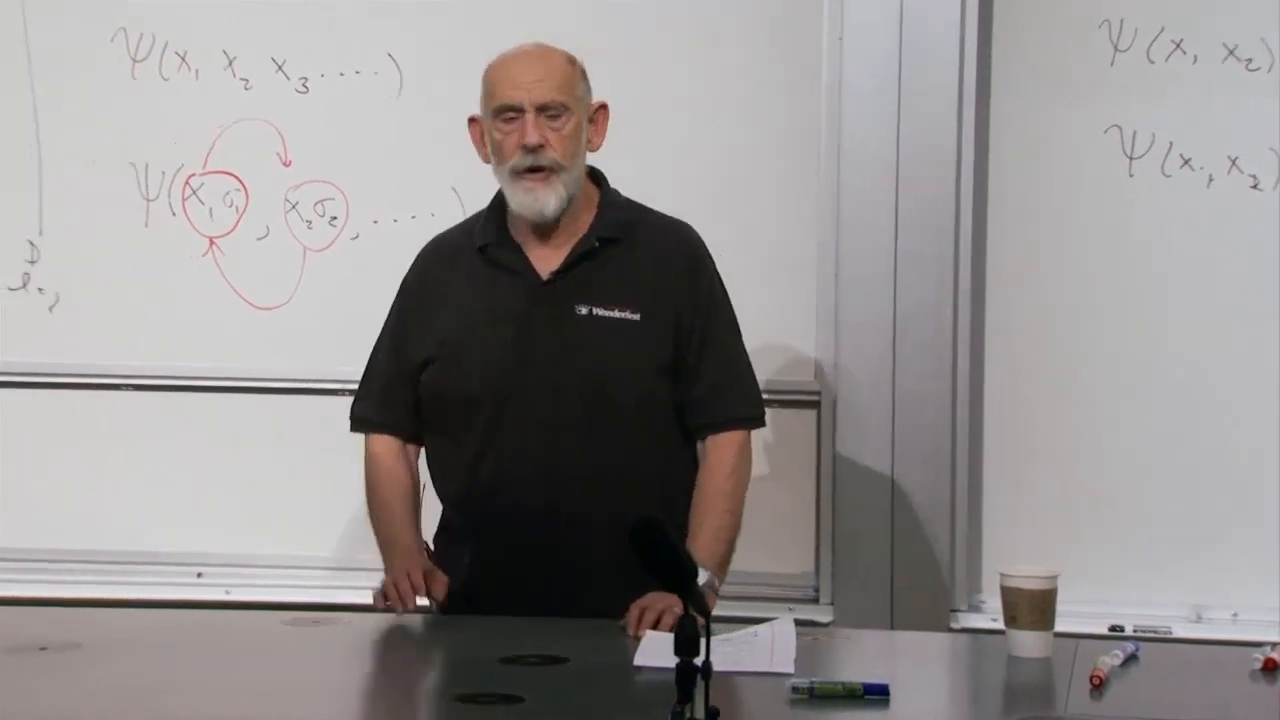
\includegraphics[width=0.9\linewidth]{lecture_05_frame_03.png}
\caption{L’échange de deux particules identiques permute leurs étiquettes complètes de position--spin. L’état bosonique reste inchangé, tandis que l’état fermionique change de signe.}
\lectureframe{00:35:25}
\end{figure}

Il s’agit de deux usages différents de la linéarité. Pour une particule,
\begin{equation}
\alpha\psi_0(x)+\beta\psi_1(x)
\end{equation}
est une superposition de deux possibilités. Pour deux particules,
\begin{equation}
\psi_0(x_1)\psi_1(x_2)
\end{equation}
est une amplitude produit dans un espace doté de deux coordonnées de particules. La symétrisation ou l’antisymétrisation combine ce produit avec son partenaire échangé.

\begin{classroomqa}
\lecturetimestamp{00:36:13}
\audiencequestion{L’échange de particules produit-il un effet d’interférence ?}
\lecturerresponse{Oui. L’annulation de l’amplitude fermionique lorsque les deux particules sont dans le même état peut se comprendre comme une interférence destructive entre les deux contributions échangées.}
\end{classroomqa}

\begin{classroomqa}
\lecturetimestamp{00:37:13}
\audiencequestion{Pauli a-t-il déduit l’exclusion à l’aide de ce même argument de symétrie ?}
\lecturerresponse{Pauli est parti d’un fait empirique et a trouvé un cadre mathématique permettant de l’exprimer. Au départ, il ne déduisait pas l’exclusion d’une théorie plus fondamentale.}
\end{classroomqa}

L’antisymétrie fournit le cadre mathématique dans lequel s’exprime la règle empirique d’exclusion.

\begin{classroomqa}
\lecturetimestamp{00:39:01}
\audiencequestion{L’interférence due à l’échange de particules est-elle liée à l’interférence entre des chemins possibles ?}
\lecturerresponse{Oui. Dans une histoire, les deux particules passent sans se croiser ; dans une autre, elles se croisent et atteignent les destinations échangées. Les amplitudes s’additionnent pour les bosons et peuvent s’annuler pour les fermions.}
\end{classroomqa}

L’échange fournit le premier signe moins. La rotation fournit le second.

\section{Le second signe moins : rotation de \texorpdfstring{\(2\pi\)}{2 pi}}

Une rotation complète semble ne rien changer. Toute direction géométrique ordinaire retrouve son orientation initiale après un angle \(2\pi\). Mais ce sont les probabilités et les valeurs moyennes qui doivent retrouver leurs valeurs initiales. Le vecteur d’état lui-même peut revenir avec une phase globale, comme cela peut aussi se produire lors d’un échange.

\begin{classroomqa}
\lecturetimestamp{00:42:12}
\audiencequestion{Quel axe utilise-t-on pour la rotation, et son générateur est-il le moment cinétique orbital, le spin, ou les deux ?}
\lecturerresponse{On peut choisir un axe extérieur ; nous prendrons ici l’axe \(z\). Le générateur est le moment cinétique total, qui comprend les contributions orbitales et de spin. Le spin lui-même n’a pas besoin d’être dirigé selon l’axe choisi.}
\end{classroomqa}

\editorialnote{Dans cette discussion, les formules du moment cinétique sont écrites avec \(\hbar=1\) ; \(m\) est donc la valeur propre sans dimension de \(J_z\).}

Soit \(\psi(\theta)\) l’état obtenu à mesure que le paramètre de rotation varie jusqu’à l’angle \(\theta\). Avec la convention utilisée ici,
\begin{equation}
J_z\psi(\theta)
=
-i\frac{\partial}{\partial\theta}\psi(\theta).
\end{equation}
Pour un état de \(J_z\) défini,
\begin{equation}
J_z\psi(\theta)=m\psi(\theta).
\end{equation}
En combinant ces équations, on obtient
\begin{equation}
-i\frac{\partial}{\partial\theta}\psi(\theta)
=
m\psi(\theta),
\end{equation}
dont la solution est
\begin{equation}
\psi(\theta)=e^{im\theta}\psi(0).
\end{equation}

Les valeurs permises de \(m\) sont des entiers ou des demi-entiers. Par conséquent,
\begin{equation}
\psi(2\pi)
=
\begin{cases}
+\psi(0), & m\in\mathbb Z,\\[4pt]
-\psi(0), & m\in\mathbb Z+\tfrac12.
\end{cases}
\end{equation}
Après un tour complet supplémentaire,
\begin{equation}
\psi(4\pi)=\psi(0)
\end{equation}
dans les deux cas. Voici le second signe moins : un état d’un multiplet de moment cinétique demi-entier change de signe lors d’une rotation de \(2\pi\).

Ce signe ne modifie pas \(\lvert\psi\rvert^2\) ; il est donc invisible lorsqu’il multiplie l’état entier. Même ainsi, une rotation de \(2\pi\) n’est pas représentée par l’identité sur un état de spin demi-entier. Cette différence devient observable lorsque le signe est relatif à une autre amplitude cohérente.

\section{Les chemins de \texorpdfstring{\(2\pi\) et \(4\pi\)}{2 pi et 4 pi}}

On peut rendre visible la différence entre \(2\pi\) et \(4\pi\) sans autre calcul. Tenez une tasse d’une main et faites-lui accomplir un tour complet sans la lâcher. La tasse retrouve son orientation initiale, mais le bras est tordu. Poursuivez d’un second tour : le bras peut alors retrouver sa position initiale sans inverser le mouvement de la tasse.

Une construction apparentée consiste à placer une sphère dans une boîte et à la relier à celle-ci par des cordes. Faire tourner la sphère de \(2\pi\) produit un enchevêtrement. Dans l’espace ordinaire à trois dimensions, l’enchevêtrement associé à un tour de \(4\pi\) peut être défait. Ce qui importe n’est pas seulement l’orientation finale de la sphère, mais le chemin parcouru dans l’espace des rotations.

\begin{classroomqa}
\lecturetimestamp{00:54:22}
\audiencequestion{Si l’on fait tourner deux fois la sphère autour du même axe, peut-on vraiment démêler les cordes ? Cela exige-t-il une dimension spatiale supplémentaire ?}
\lecturerresponse{Le chemin de \(4\pi\) peut être défait dans l’espace ordinaire à trois dimensions. Le temps paramètre le mouvement ; ce n’est pas une direction spatiale supplémentaire. Un chemin de \(2\pi\) ne peut pas être défait de cette façon, contrairement à un chemin de \(4\pi\).}
\end{classroomqa}

Les démonstrations distinguent un chemin de \(2\pi\) non trivial d’un chemin de \(4\pi\) que l’on peut défaire, sans élaborer de théorie formelle du groupe des rotations.

\section{Échange et rotation dans la représentation par une ceinture}

Les deux signes moins apparaissent maintenant côte à côte. L’échange de deux fermions identiques change le signe de leur fonction d’onde conjointe. La rotation d’un état de spin demi-entier de \(2\pi\) change elle aussi son signe. Une ceinture établit un lien géométrique entre ces deux opérations.

Disposez la ceinture de sorte que ses deux extrémités inférieures aient été échangées. Considérée autrement, la même ceinture présente une torsion de \(2\pi\). Effectuer l’échange en même temps que la rotation de \(2\pi\) supprime la torsion et laisse une ceinture sans torsion. Le processus combiné peut être ramené continûment à l’absence de toute opération.\footnote{Dans le cours, l’observation reliant l’échange--à la rotation est attribuée à David Finkelstein. La source ne précise aucune publication ; son nom est donc conservé ici uniquement comme attribution.}

\begin{classroomqa}
\lecturetimestamp{01:01:12}
\audiencequestion{S’agit-il seulement d’une affirmation sur la façon dont la ceinture est plongée dans l’espace, plutôt que d’une affirmation sur la topologie des particules ?}
\lecturerresponse{On peut interpréter la ceinture comme l’histoire d’une particule dans l’espace-temps. Si le temps s’écoule vers le haut, une coupe transversale fait apparaître des objets semblables à des particules. Des paires sont créées, un objet subit une rotation de \(2\pi\), puis deux objets identiques sont échangés. Dans cette histoire, les phases de rotation et d’échange s’annulent.}
\end{classroomqa}

Cette histoire rend explicite le calcul des phases. Partons d’une situation sans particule. En deux endroits distincts, créons une paire particule--antiparticule, ce qui laisse quatre particules à un instant intermédiaire. Faisons subir à l’une d’elles une rotation de \(2\pi\), tout en échangeant deux particules identiques ailleurs dans la configuration. L’histoire complète peut être déformée en l’histoire élémentaire où une paire est créée puis annihilée. Dans le calcul des signes considéré ici, cette histoire triviale n’ajoute aucune phase. Si \(\eta_{\mathrm{rot}}\) et \(\eta_{\mathrm{ex}}\) désignent les deux signes, l’annulation évoquée peut s’écrire simplement ainsi :\footnote{Cette équation de phase consigne l’annulation décrite entre 01:06:50 et 01:07:18 ; le cours présente cette construction comme suggestive, et non comme une preuve rigoureuse.}
\begin{equation}
\eta_{\mathrm{rot}}\eta_{\mathrm{ex}}=1.
\end{equation}

\begin{classroomqa}
\lecturetimestamp{01:03:34}
\audiencequestion{Peut-on relier l’échange aux rotations en faisant parcourir \(\pi\) à chacune de deux particules, puis en les réorientant ?}
\lecturerresponse{Cette construction peut faire intervenir des mathématiques apparentées, mais elle utilise deux rotations distinctes de \(\pi\). Le processus étudié ici comporte une seule rotation de \(2\pi\) ; les deux arguments ne sont donc pas identiques.}
\end{classroomqa}

L’argument repose sur la possibilité de créer et d’annihiler des objets semblables à des particules. Il ne prendrait pas cette forme dans une théorie où les particules seraient éternelles. Il n’est pas non plus présenté comme la preuve habituelle du théorème spin--statistiques. Son objectif est de mettre en évidence une raison topologique pour laquelle les signes associés à l’échange et à la rotation sont compatibles.

\section{Lumps, images miroir et annihilation}

On peut répéter la construction avec des configurations de champs localisées. Supposons qu’un ou plusieurs champs prennent presque partout leurs valeurs dans le vide, mais présentent une forme et une structure non nulles dans une petite région. Cette configuration localisée est un lump.

Construisons maintenant une seconde configuration, image miroir appropriée de la première. Appelons l’une la particule et l’autre l’antiparticule. Rapprochons-les. Les parties correspondantes des configurations de champs se rencontrent et s’annulent mutuellement. À une étape intermédiaire, certaines parties des lumps peuvent déjà avoir disparu tandis que d’autres subsistent. En poursuivant la déformation, on élimine la structure restante et l’on ramène les champs à la configuration du vide. Deux torsions orientées en sens opposés dans une ceinture donnent la même image : rapprochez-les par poussée et elles se défont.

On peut inverser le processus. L’espace vide peut produire un lump et son partenaire miroir. On peut créer deux paires de ce type, faire subir à un lump une rotation de \(2\pi\), échanger deux lumps identiques, puis annihiler de nouveau les paires. La même annulation entre échange--et rotation s’applique alors. Cette extension de la construction reste heuristique ; ce n’est pas un théorème concernant toute excitation localisée.

\begin{classroomqa}
\lecturetimestamp{01:11:30}
\audiencequestion{Existe-t-il des réalisations physiques de ces configurations de champs semblables à des lumps ?}
\lecturerresponse{Oui. On peut citer les noyaux dans les descriptions de type Skyrmion, les monopôles magnétiques et d’autres excitations des champs semblables à des particules.}
\end{classroomqa}

L’image des lumps miroirs rend la généralisation intelligible. Ce qui compte, ce n’est pas que l’objet ait été initialement une particule ponctuelle élémentaire, mais qu’une excitation semblable à une particule et son partenaire puissent être créés, rapprochés et annihilés de façon continue. Cette propriété motive une relation plus générale entre le comportement sous rotation et sous échange.

\begin{classroomqa}
\lecturetimestamp{01:16:12}
\audiencequestion{Le spin un demi signifie-t-il que l’état n’accumule que la moitié de la phase de rotation habituelle ?}
\lecturerresponse{Dans cette convention, la phase est \(e^{im\theta}\). Pour un \(m\) demi-entier, une rotation de \(2\pi\) donne \(-1\), tandis qu’une rotation de \(4\pi\) donne \(+1\).}
\end{classroomqa}

\section{Un signe global et une expérience nulle}

Peut-on observer le signe moins issu d’une rotation de \(2\pi\) ? Commençons par une expérience où ce n’est pas possible. Piégeons un électron dans un champ magnétique, laissons son spin suivre le champ tandis que l’appareil tourne lentement de \(2\pi\), puis libérons l’électron dans un dispositif d’interférence. Comparons cela à la même procédure sans rotation.

La rotation transforme l’état selon
\begin{equation}
\psi\longmapsto-\psi,
\end{equation}
mais le signe moins multiplie l’état entier. Toutes les probabilités restent inchangées ; la figure d’interférence finale ne conserve donc aucune trace de la rotation préalable. C’est une expérience nulle : une phase commune n’a rien avec quoi interférer.

\begin{classroomqa}
\lecturetimestamp{01:20:01}
\audiencequestion{Pourquoi faut-il faire tourner lentement le champ magnétique ?}
\lecturerresponse{Le spin doit continuer à suivre le champ magnétique en rotation. Si le champ est entraîné trop rapidement, le spin ne restera pas aligné sur lui.}
\end{classroomqa}

\section{Un électron dans deux branches cohérentes}

Le signe devient observable lorsqu’il est rendu relatif. Faisons passer un électron dans un séparateur de faisceau. Une partie de sa fonction d’onde suit un trajet, l’autre partie un second trajet :
\begin{equation}
\psi(x)=\psi_1(x)+\psi_2(x).
\end{equation}
Il s’agit d’un seul électron, pas de deux électrons. C’est une superposition cohérente de deux possibilités. Il faut bien garder cette distinction à l’esprit : les deux paquets ne sont pas deux particules indépendantes.

Dirigeons les deux paquets vers des régions distinctes contenant des champs magnétiques. Dans l’une, faisons tourner le champ de \(2\pi\), sans modifier l’autre. Pour un état de spin demi-entier,
\begin{equation}
\psi_1(x)+\psi_2(x)
\longmapsto
\psi_1(x)-\psi_2(x),
\end{equation}
où l’on a choisi \(2\) comme étiquette de la branche ayant subi la rotation. Le signe est maintenant relatif. Lorsque les deux paquets se recouvrent plus tard, l’addition devient une soustraction. Un point d’interférence constructive peut devenir un point d’interférence destructive, voire un nœud.

\begin{classroomqa}
\lecturetimestamp{01:23:46}
\audiencequestion{Que fait-on tourner s’il n’y a qu’un électron mais deux branches de la fonction d’onde ?}
\lecturerresponse{L’électron est dans une superposition cohérente de deux possibilités localisées. On fait subir une rotation à une branche, pas à l’autre. Si l’on ouvre les boîtes pour savoir laquelle des deux possibilités s’est réalisée, cette mesure détruit l’interférence.}
\end{classroomqa}

Ouvrir les boîtes ne révélerait qu’un seul électron, dans l’une ou l’autre. Sans cette mesure, les deux amplitudes restent présentes dans l’état. La répétition de l’expérience fait apparaître la figure d’interférence détection après détection. Au nœud produit par le signe moins relatif, aucun électron n’est détecté.

\section{Précession magnétique et interférence à deux fentes}

Un dispositif schématique plus pratique remplace l’expérience des boîtes, qui exigerait un mouvement très lent. Séparons une onde électronique cohérente en deux trajets. Sur l’un d’eux, faisons passer l’électron dans une région magnétique alors que son spin est initialement transverse au champ. Le spin entre alors en précession. En choisissant l’intensité du champ et le temps de traversée, on peut faire accomplir au spin de cette branche un tour complet de \(2\pi\), tandis que l’autre branche n’effectue aucun tour de ce type.\footnote{Le cours indique qu’une expérience apparentée sur la phase des spineurs a été réalisée et en décrit le principe, mais la source ne précise ni publication ni dispositif particulier. Le compte rendu se limite donc à la construction présentée dans le cours.}

\begin{classroomqa}
\lecturetimestamp{01:27:05}
\audiencequestion{Comment peut-on déterminer le trajet suivi par l’électron unique ?}
\lecturerresponse{On ne le peut pas sans compromettre l’expérience. Toute mesure qui enregistre le trajet suivi par l’électron détruit l’interférence.}
\end{classroomqa}

\begin{classroomqa}
\lecturetimestamp{01:27:50}
\audiencequestion{Qu’est-ce exactement qu’une branche de la fonction d’onde, et comment le séparateur en produit-il deux ?}
\lecturerresponse{Une branche est un paquet d’ondes localisé le long d’un trajet. Le séparateur transforme l’onde incidente en deux paquets spatialement séparés, que des champs électriques ou magnétiques peuvent guider sur des trajets différents.}
\end{classroomqa}

À part la région magnétique, il s’agit de l’expérience à deux fentes. Une onde électronique incidente se sépare en deux paquets. Les ondes sortantes s’étalent dans une région de détection commune, où leurs amplitudes se recouvrent. En l’absence de rotation relative, les amplitudes centrales peuvent s’additionner. Une rotation de spin de \(2\pi\) sur l’un des trajets inverse une amplitude et peut annuler ces mêmes contributions.

\begin{classroomqa}
\lecturetimestamp{01:30:46}
\audiencequestion{Comment peut-il y avoir interférence si l’électron emprunte des tubes ou des fentes distincts ?}
\lecturerresponse{La détection finale ne révèle pas le trajet. Les deux amplitudes d’onde sortantes s’étalent et se recouvrent au détecteur. Chercher à déterminer le trajet suivi détruirait l’interférence.}
\end{classroomqa}

\begin{classroomqa}
\lecturetimestamp{01:33:22}
\audiencequestion{Le diamètre du tube ou de la fente doit-il être comparable à la longueur d’onde de l’électron ?}
\lecturerresponse{Dans une réalisation littérale de l’expérience à deux fentes fondée sur la diffraction, l’ouverture doit être assez petite pour produire l’étalement nécessaire. Le dispositif décrit est schématique et ne constitue pas un plan expérimental pratique.}
\end{classroomqa}

\begin{classroomqa}
\lecturetimestamp{01:33:44}
\audiencequestion{Une rotation de polarisation correspondante des photons de \(2\pi\) laisserait-elle la figure d’interférence inchangée ?}
\lecturerresponse{Oui. Les photons ont un spin entier ; une rotation complète de \(2\pi\) n’introduit donc pas le signe moins propre aux fermions.}
\end{classroomqa}

\begin{classroomqa}
\lecturetimestamp{01:34:12}
\audiencequestion{En quoi l’expérience pratique s’écarte-t-elle légèrement de la version idéalisée ?}
\lecturerresponse{Dans le dispositif idéal, le spin tourne de manière adiabatique. Dans la description pratique, l’électron traverse une région magnétique et son spin précesse plus rapidement, mais la phase mesurée reste celle qui est associée à un tour de \(2\pi\).}
\end{classroomqa}

Le dispositif lent isole l’idée en veillant à ce que le spin suive le champ sans mouvement supplémentaire. Le dispositif fondé sur la précession produit dynamiquement le même signe relatif. Dans les deux versions, les deux trajets doivent cesser d’être distinguables pour qu’une figure d’interférence puisse apparaître.

\begin{classroomqa}
\lecturetimestamp{01:36:15}
\audiencequestion{Faut-il recombiner les deux branches après le séparateur ?}
\lecturerresponse{Oui. Les paquets d’ondes qui émergent doivent se recouvrir, ou s’étendre sur une même région de détection, afin que leurs amplitudes puissent former une figure d’interférence.}
\end{classroomqa}

\begin{classroomqa}
\lecturetimestamp{01:38:12}
\audiencequestion{Cette expérience de rotation avec un seul électron découle-t-elle du principe d’exclusion de Pauli ?}
\lecturerresponse{Non. Il n’y a qu’un seul électron. L’expérience mesure la phase du spineur lors d’une rotation, et non l’exclusion de deux fermions d’un même état.}
\end{classroomqa}

\section{Interférence par échange et rotation relative}

On pourrait mettre en évidence un signe d’échange par la même méthode générale, bien que l’appareillage proposé soit plus complexe. On commence par deux électrons et l’on sépare leur fonction d’onde commune en deux branches cohérentes. Il n’y a toujours que deux électrons, et non quatre : la paire suit l’une ou l’autre des deux possibilités. Dans une branche, on échange les deux électrons ; dans l’autre, on ne les échange pas. Une fois les branches recombinées, le signe d’échange fermionique apparaît comme une phase relative et peut modifier les interférences.

La proposition finale compare directement les deux signes moins. Une branche acquiert la phase d’échange fermionique, tandis que l’autre acquiert la phase correspondante à une rotation de \(2\pi\). Les deux phases valent \(-1\), si bien que leurs effets relatifs s’annulent.\footnote{L’enregistrement entre 01:40:26 et 01:41:15 montre clairement une phase d’échange, une phase correspondant à une rotation de \(2\pi\) et leur annulation, mais les paroles disponibles ne permettent pas de déterminer à quoi la rotation est précisément attribuée.} Le cours présente cela comme une expérience de pensée proposée et précise qu’à la connaissance de l’intervenant, elle n’avait pas été réalisée.

\begin{classroomqa}
\lecturetimestamp{01:41:34}
\audiencequestion{L’observation d’une phase d’échange remettrait-elle en question l’indiscernabilité des deux électrons ?}
\lecturerresponse{Non. L’indiscernabilité quantique est plus subtile que la similitude classique. Elle permet au vecteur d’état de changer de signe lors d’un échange, même si aucune étiquette observable ne distingue les particules.}
\end{classroomqa}

Il reste une dernière réserve. Faire tourner un monde entier isolé de \(2\pi\) ne produirait qu’une phase commune, qu’aucune expérience interne ne pourrait révéler. L’expérience détectable consiste à faire tourner une branche cohérente par rapport à une autre. Ce qui est observé n’est donc pas un signe absolu, mais les interférences produites par un signe relatif.

\chapter{Oscillateurs, nombres d’occupation et premier champ quantique}

La théorie quantique des champs est le cadre qui décrit pratiquement toute la physique non gravitationnelle connue. Cette affirmation ne signifie pas que tous les problèmes peuvent être résolus. L’atome d’hydrogène est accessible au calcul ; dès que l’on considère un atome comme le bore, le calcul devient déjà bien plus difficile, et celui d’un être humain dépasse de très loin toute capacité réaliste de calcul en théorie des champs. Le cadre peut être fondamental alors même que ses équations restent extrêmement difficiles à résoudre.

Nous allons donc aborder le sujet de la manière la plus élémentaire possible. On l’appelle parfois \emph{seconde quantification}, mais ce nom n’aura guère de sens tant que nous n’aurons pas construit les outils nécessaires. Le chemin le plus court ne part pas d’un champ relativiste, mais de l’oscillateur harmonique. Les ressorts ne sont pas l’essentiel. Ce qui compte, c’est l’algèbre des opérateurs de création et d’annihilation. Dès que l’on répète cette algèbre pour de nombreux modes, un opérateur de création ne signifiera plus simplement ``faire monter un oscillateur d’un niveau'', mais littéralement ``créer une particule.''

\section{L’oscillateur vu comme une algèbre}

Pour un oscillateur, notons \(a^\dagger\) l’opérateur qui augmente l’excitation et \(a\) celui qui la diminue. Les notations \(a_+\) et \(a_-\) sont équivalentes, mais la notation avec dagues anticipe le langage de la théorie des champs. L’état fondamental vérifie
\begin{equation}
a|0\rangle=0,
\end{equation}
et l’opérateur nombre est
\begin{equation}
N=a^\dagger a,
\qquad
N|n\rangle=n|n\rangle.
\end{equation}
Les deux opérateurs d’échelle sont adjoints l’un de l’autre, et leur commutateur essentiel est
\begin{equation}
[a,a^\dagger]=1.
\label{eq:l06-single-commutator}
\end{equation}
Cette petite algèbre constitue presque toute la théorie de l’oscillateur.

On peut retrouver \(a\) et \(a^\dagger\) à partir de combinaisons linéaires appropriées de la position et de l’impulsion. La convention précise dépend des normalisations de \(x\), \(p\), \(m\) et \(\omega\) ; l’énoncé invariant utile ici est que \(a^\dagger a\) reconstitue l’hamiltonien quadratique de l’oscillateur, à une constante additive égale à l’énergie de l’état fondamental près. Ainsi,
\begin{equation}
H=\hbar\omega\left(N+\frac12\right).
\end{equation}
Dans la suite, nous omettons le terme constant et considérons
\begin{equation}
H=\hbar\omega N.
\label{eq:l06-one-oscillator-hamiltonian}
\end{equation}
La fréquence détermine le coût d’une excitation. Augmenter \(n\) d’une unité coûte \(\hbar\omega\) ; diminuer \(n\) d’une unité libère la même quantité d’énergie.

\section{Oscillateurs indépendants en grand nombre}

Considérons maintenant de nombreux oscillateurs, indicés par \(i\). Cet indice n’est qu’un indice, et non l’unité imaginaire. Il peut y avoir un nombre fini ou infini de modes. Un ensemble de ressorts indépendants en donne une image ; les modes normaux d’une corde de violon idéale en donnent une autre. En théorie des champs, c’est le cas d’une infinité de modes qui importe.

L’indépendance a un sens opératoriel. Les opérateurs associés à des sous-systèmes réellement indépendants commutent. Dans le cas contraire, les grandeurs correspondantes ne pourraient pas être mesurées indépendamment et les systèmes ne seraient pas indépendants au départ. Nous avons donc
\begin{align}
[a_i,a_j]&=0, \\
[a_i^\dagger,a_j^\dagger]&=0, \\
[a_i,a_j^\dagger]&=\delta_{ij}.
\label{eq:l06-many-commutators}
\end{align}
Pour \(i\ne j\), tous les opérateurs associés aux deux modes commutent. Pour \(i=j\), la dernière ligne se réduit à l’équation~\eqref{eq:l06-single-commutator}.

Chaque oscillateur possède son propre opérateur nombre et, en général, sa propre fréquence :
\begin{equation}
N_i=a_i^\dagger a_i,
\qquad
H=\sum_i\hbar\omega_i N_i.
\label{eq:l06-many-hamiltonian}
\end{equation}
Un état propre simultané est spécifié par la liste complète
\begin{equation}
|n_1,n_2,n_3,\ldots\rangle,
\qquad n_i=0,1,2,\ldots.
\label{eq:l06-occupation-ket}
\end{equation}
L’entier \(n_i\) est appelé le \emph{nombre d’occupation} du \(i\)e oscillateur. Pour l’instant, ce n’est qu’un terme. Bientôt, il comptera les particules qui occupent un état à une particule, et le nom prendra son sens littéral.

L’état dont tous les nombres d’occupation sont nuls est
\begin{equation}
|0\rangle\equiv|0,0,0,\ldots\rangle,
\qquad a_i|0\rangle=0\quad\text{for every }i.
\label{eq:l06-oscillator-vacuum}
\end{equation}

\begin{classroomqa}\lecturetimestamp{00:15:27}\audiencequestion{Une famille infinie d’oscillateurs correspond-elle au continuum de modes d’un système comme une corde de violon ?}\lecturerresponse{Oui, dans le modèle idéalisé de la corde. Une corde réelle est constituée d’atomes, de sorte que les longueurs d’onde suffisamment courtes finissent par atteindre une coupure microscopique. Le modèle continu motive néanmoins l’ensemble infini de modes utilisé en théorie des champs.}\end{classroomqa}

\section{Pourquoi les coefficients d’échelle sont des racines carrées}

L’action de \(a^\dagger\) doit faire passer un état propre de \(N\) à l’état propre suivant, mais la normalisation laisse place à un coefficient :
\begin{equation}
a^\dagger|n\rangle=c_n|n+1\rangle.
\label{eq:l06-unknown-coefficient}
\end{equation}

\begin{figure}[htbp]\centering
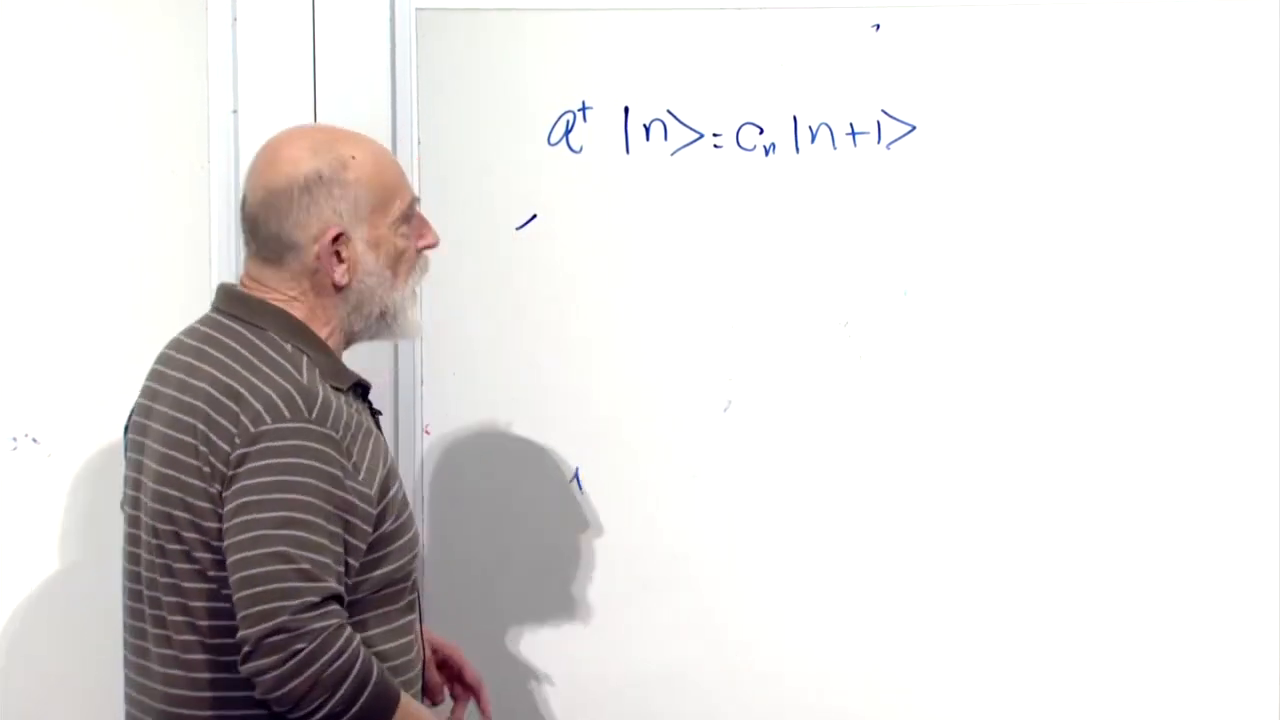
\includegraphics[width=0.9\linewidth]{lecture_06_frame_01.png}\caption{Le coefficient d’échelle est introduit avant que sa normalisation soit établie. L’équation inscrite au tableau est reproduite dans l’équation~\eqref{eq:l06-unknown-coefficient}.}\lectureframe{00:19:38}\end{figure}

Adoptons la convention de phase selon laquelle \(c_n\) est réel. En prenant l’adjoint hermitien, on obtient
\begin{equation}
\langle n|a=c_n\langle n+1|.
\end{equation}
En multipliant les deux relations et en utilisant la normalisation des états de base,
\begin{align}
c_n^2
&=\langle n|aa^\dagger|n\rangle \\
&=\langle n|(a^\dagger a+1)|n\rangle \\
&=\langle n|(N+1)|n\rangle \\
&=n+1.
\end{align}
Par conséquent,
\begin{equation}
a^\dagger|n\rangle=\sqrt{n+1}\,|n+1\rangle.
\label{eq:l06-raising-rule}
\end{equation}

\begin{classroomqa}\lecturetimestamp{00:22:35}\audiencequestion{Pourquoi peut-on poser \(\langle n+1|n+1\rangle=1\) avant de déterminer \(c_n\) ?}\lecturerresponse{Les vecteurs propres sont choisis dès le départ comme une base normalisée. Leur normalisation ne détermine pas celle de \(a^\dagger|n\rangle\) ; l’information qui reste à fixer est précisément le coefficient \(c_n\).}\end{classroomqa}

La règle d’abaissement s’obtient de la même manière :
\begin{equation}
a|n\rangle=\sqrt n\,|n-1\rangle.
\label{eq:l06-lowering-rule}
\end{equation}
Pour \(n=0\), le coefficient s’annule automatiquement ; la règle inclut donc \(a|0\rangle=0\). Avec plusieurs modes, l’opérateur ne modifie que le nombre d’occupation à son propre emplacement :
\begin{align}
a_i^\dagger|n_1,\ldots,n_i,\ldots\rangle
&=\sqrt{n_i+1}\,|n_1,\ldots,n_i+1,\ldots\rangle, \\
a_i|n_1,\ldots,n_i,\ldots\rangle
&=\sqrt{n_i}\,|n_1,\ldots,n_i-1,\ldots\rangle.
\label{eq:l06-multimode-ladders}
\end{align}
Les autres entrées restent inchangées.

\section{Une fonction d’onde n’est pas un champ quantique}

Avant de définir un champ, nous devons le distinguer de la fonction d’onde habituelle. Trois différences organisent cette transition.

Premièrement, une fonction d’onde à une particule
\begin{equation}
\psi(x)=\langle x|\psi\rangle
\end{equation}
est une représentation d’un vecteur d’état. Ce n’est pas une observable en soi. Nous mesurons la position, l’impulsion, le moment cinétique et d’autres opérateurs ; la fonction d’onde fournit les amplitudes à partir desquelles on calcule les probabilités de ces résultats.

Deuxièmement, la fonction d’onde à plusieurs particules dépend des positions de toutes les particules. Pour deux particules dont les vecteurs position sont provisoirement notés \(x\) et \(y\),
\begin{equation}
\psi(x,y)=\langle x,y|\psi\rangle.
\end{equation}
Ici, \(x\) et \(y\) désignent deux particules différentes ; ce ne sont pas les composantes cartésiennes \(x\) et \(y\) d’un même vecteur position. Pour \(N\) particules, l’état est représenté par
\begin{equation}
\psi(x_1,x_2,\ldots,x_N).
\end{equation}

Troisièmement, cette fonction d’onde décrit un nombre fixe de particules. Une fonction d’onde à quinze particules dépend de quinze variables de position et appartient à un espace de Hilbert à quinze particules. À elle seule, elle ne décrit pas un processus où le nombre de particules passe de quinze à quatorze ou à seize.

Un champ quantique inverse ces caractéristiques. C’est un opérateur plutôt qu’un état ; il dépend d’un seul point de l’espace \(x\) et agit sur un espace d’états qui contient tous les secteurs de nombre de particules. L’expression ``un point'' désigne un vecteur position libre de varier. Elle ne signifie pas qu’une valeur numérique unique a été attribuée à \(x\).

Une réserve sera importante par la suite. Le champ \(\Psi(x)\) introduit ci-dessous n’est pas hermitien ; il n’est donc pas lui-même une observable au sens strict. Ses combinaisons hermitiennes sont des observables. L’affirmation provisoire selon laquelle un champ est mesurable est donc précisée, et non abandonnée : les champs sont des fonctions à valeurs opératorielles, et leurs combinaisons hermitiennes représentent des grandeurs mesurables.

\begin{classroomqa}\lecturetimestamp{00:36:52}\audiencequestion{Si le champ est une fonction d’une position, cette position peut-elle varier ? Et qu’est-il advenu de \(y\) dans la fonction d’onde à deux particules ?}\lecturerresponse{Le point \(x\) parcourt tout l’espace. ``Un point'' signifie que l’opérateur dépend d’un seul argument spatial, et non que cet argument est fixé. Dans \(\psi(x,y)\), les symboles \(x\) et \(y\) désignent les positions de deux particules ; on peut aussi les noter \(x_1\) et \(x_2\). Ce ne sont pas deux composantes cartésiennes de l’argument du champ.}\end{classroomqa}

\begin{classroomqa}\lecturetimestamp{00:38:15}\audiencequestion{Quel est le lien entre les descriptions par fonction d’onde à nombre fixe de particules et par champ ? Décrivent-elles des sortes de particules différentes ?}\lecturerresponse{Le lien est la construction centrale que nous allons encore établir. Les particules sont de même nature. Dans ce cours, ce sont des bosons ; les fermions nécessitent une algèbre différente.}\end{classroomqa}

\section{Une particule dans une boîte}

Revenons provisoirement à la mécanique quantique ordinaire à une particule. Plaçons une particule dans une boîte unidimensionnelle. Avec une seule particule, la distinction entre boson et fermion est sans importance : il n’y a pas de seconde particule identique permettant de tester l’échange ou le principe d’exclusion.

Soient
\begin{equation}
\psi_1(x),\ \psi_2(x),\ \psi_3(x),\ldots
\end{equation}
les fonctions propres de l’énergie. Le mode le plus bas est l’onde la plus lisse qui s’annule aux parois. Le mode suivant possède un nœud intérieur, et les modes d’énergie plus élevée oscillent plus rapidement. Pour un puits carré infini idéal de largeur \(L\), une base orthonormée commode est
\begin{equation}
\psi_i(x)=\sqrt{\frac{2}{L}}\sin\!\left(\frac{i\pi x}{L}\right),
\qquad 0<x<L.
\label{eq:l06-box-basis}
\end{equation}
La formule explicite en sinus est une réalisation standard du schéma qualitatif tracé au tableau ; l’argument qui suit ne requiert qu’un ensemble complet d’états à une particule orthonormés.

\begin{figure}[htbp]\centering
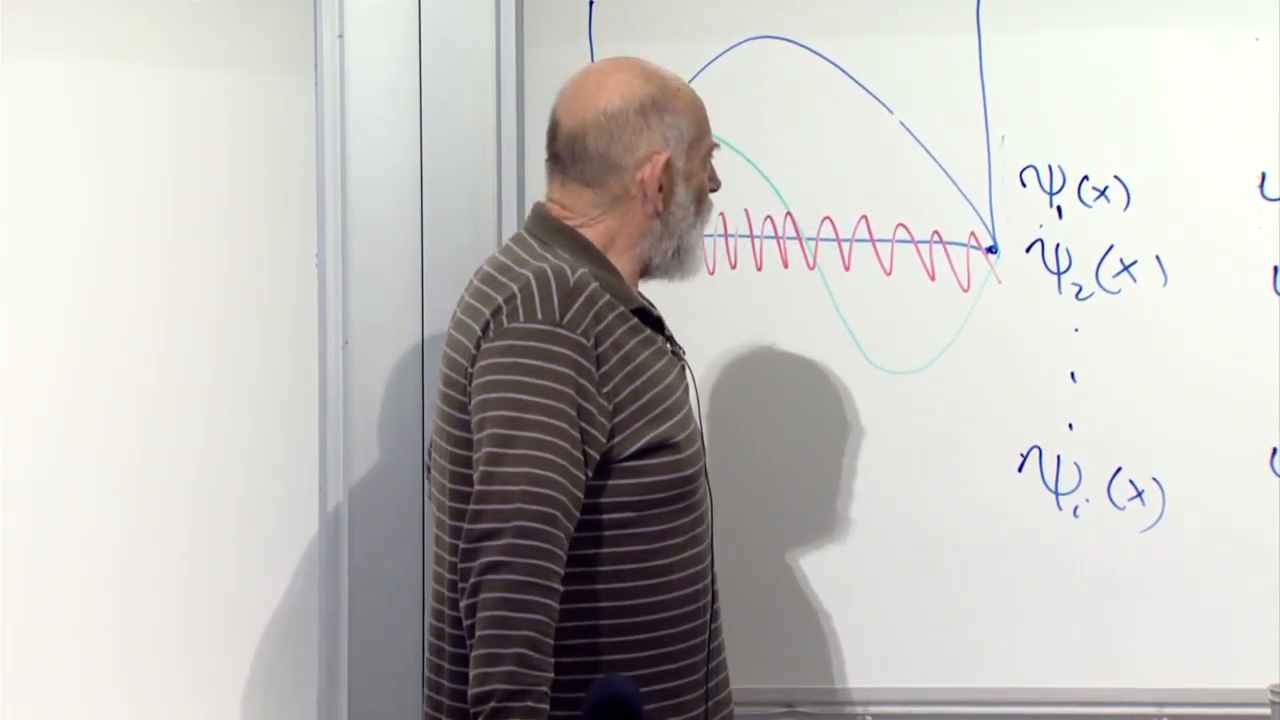
\includegraphics[width=0.9\linewidth]{lecture_06_frame_03.png}\caption{Modes d’une particule dans une boîte, classés par énergie croissante. Le premier mode n’a aucun nœud intérieur, le deuxième en a un, et les modes supérieurs omis oscillent de plus en plus rapidement.}\lectureframe{00:43:10}\end{figure}

La même structure peut être représentée à nouveau sans l’occultation du tableau en direct :
\begin{figure}[htbp]\centering
\begin{tikzpicture}[x=1cm,y=1cm]
  \draw[thick] (0,0) -- (0,3.8);
  \draw[thick] (7,0) -- (7,3.8);
  \draw[gray!55] (0,2.75) -- (7,2.75);
  \draw[gray!55] (0,1.35) -- (7,1.35);
  \draw[blue!75!black,thick,domain=0:7,samples=120]
    plot (\x,{2.75+0.62*sin(180*\x/7)});
  \draw[teal!70!black,thick,domain=0:7,samples=120]
    plot (\x,{1.35+0.55*sin(360*\x/7)});
  \node[right] at (7.15,3.15) {$\psi_1(x)$};
  \node[right] at (7.15,1.70) {$\psi_2(x)$};
  \node at (3.5,0.45) {$\vdots\quad \psi_i(x)$};
\end{tikzpicture}\caption{Reconstitution nette du schéma qualitatif des modes dans la boîte. Le décalage vertical sépare les fonctions propres pour en faciliter la lecture ; il ne représente pas une coordonnée physique supplémentaire.}\end{figure}

L’indice \(i\) repère un état à une particule, et non une particule ni le nombre de nœuds. Pour la base de la boîte, \(i\) vaut par coïncidence un de plus que le nombre de nœuds intérieurs. Chaque état possède une énergie \(\varepsilon_i\). En suivant la notation du cours, nous pouvons noter cette énergie \(\hbar\omega_i\), ou simplement \(\omega_i\) après avoir posé \(\hbar=1\).

\begin{classroomqa}\lecturetimestamp{00:39:01}\audiencequestion{L’hypothèse d’indépendance formulée plus tôt était-elle exacte, et l’indice \(i\) pourrait-il désigner les états possibles d’un électron dans un atome ?}\lecturerresponse{Dans la construction à modes indépendants, les relations de commutation entre modes différents sont exactes. L’indice peut désigner des états atomiques à une particule. Toutefois, si les particules interagissent, l’hamiltonien simple à modes indépendants ne suffit plus à décrire le système.}\end{classroomqa}

\begin{classroomqa}\lecturetimestamp{00:40:34}\audiencequestion{La particule dans la boîte est-elle un boson ?}\lecturerresponse{C’est possible, mais avec une seule particule, la statistique n’a pas d’importance. Le principe d’exclusion et l’échange ne prennent sens qu’en présence de plusieurs particules identiques.}\end{classroomqa}

\section{Des modes de la boîte à l’espace de Fock}

Autorisons maintenant un nombre quelconque de bosons identiques dans la boîte. Un certain nombre \(n_1\) peut occuper \(\psi_1\), un certain nombre \(n_2\) peut occuper \(\psi_2\), et ainsi de suite. Un état de base s’écrit donc
\begin{equation}
|n_1,n_2,n_3,\ldots\rangle.
\end{equation}
C’est exactement la notation déjà utilisée pour plusieurs oscillateurs. L’identité est structurelle : associons un oscillateur à chaque état à une particule et identifions le nombre d’excitations de l’oscillateur au nombre de particules qui occupent cet état.

Les bosons sont essentiels ici, car chaque \(n_i\) peut être n’importe quel entier non négatif. Pour les fermions, chaque état à une particule peut être vide ou occupé par une seule particule, jamais par deux ; l’algèbre ordinaire de l’oscillateur ne peut donc pas être reprise telle quelle.

On peut maintenant définir les opérateurs par leur action sur la base des nombres d’occupation. L’opérateur \(a_i^\dagger\) crée une particule dans l’état à une particule \(i\) ; \(a_i\) en enlève une :
\begin{align}
a_i^\dagger|n_1,\ldots,n_i,\ldots\rangle
&=\sqrt{n_i+1}\,|n_1,\ldots,n_i+1,\ldots\rangle, \\
a_i|n_1,\ldots,n_i,\ldots\rangle
&=\sqrt{n_i}\,|n_1,\ldots,n_i-1,\ldots\rangle.
\end{align}
Ce n’est pas une analogie introduite après coup. C’est la définition des opérateurs bosoniques de création et d’annihilation sur cette base. Comme la base engendre l’espace, cette définition détermine leur action sur tout état par linéarité.

\begin{classroomqa}\lecturetimestamp{00:47:11}\audiencequestion{Les \(n_1,n_2,n_3\) sont-ils les états quantiques ?}\lecturerresponse{Les indices \(1,2,3,\ldots\) identifient les états à une particule. Les symboles \(n_1,n_2,n_3,\ldots\) indiquent le nombre de particules qui occupent ces états. Distinguer l’étiquette d’un état de son nombre d’occupation constitue la principale difficulté de notation.}\end{classroomqa}

\subsection{Le rôle de la racine carrée}

Le facteur \(\sqrt{n_i+1}\) ne représente ni une particule supplémentaire ni un processus physique distinct. Il donne à l’opérateur la normalisation et l’algèbre appropriées. Pour un mode,
\begin{align}
a a^\dagger|n\rangle
&=a\bigl(\sqrt{n+1}\,|n+1\rangle\bigr) \\
&=(n+1)|n\rangle,
\end{align}
tandis que
\begin{equation}
a^\dagger a|n\rangle=n|n\rangle.
\end{equation}
Leur différence est donc \(|n\rangle\), comme l’exige \([a,a^\dagger]=1\). En gros, chacun des deux opérateurs d’échelle est d’ordre \(\sqrt n\), puisque leur produit donne l’opérateur nombre, d’ordre \(n\).

\begin{classroomqa}\lecturetimestamp{00:47:52}\audiencequestion{Quelle signification physique concrète faut-il attribuer au facteur racine carrée ?}\lecturerresponse{Il s’agit avant tout d’une normalisation mathématique. Elle garantit que les états d’occupation sont normalisés, que \(a^\dagger a\) a pour valeur propre \(n\) et que les opérateurs d’échelle vérifient le commutateur de l’oscillateur. Parfois, les mathématiques constituent à elles seules le sens dont on a besoin.}\end{classroomqa}

\begin{classroomqa}\lecturetimestamp{00:52:25}\audiencequestion{Les opérateurs de création et d’annihilation ont-ils été définis uniquement par leurs propriétés et leur action sur la base ?}\lecturerresponse{Oui. Les définitions n’ont pas à découler d’une représentation plus fondamentale. Leur intérêt se mesure à leurs conséquences. Définir l’action sur une base complète définit les opérateurs partout, et ces définitions reproduisent les relations de commutation voulues.}\end{classroomqa}

\begin{classroomqa}\lecturetimestamp{00:53:22}\audiencequestion{Pourquoi \(a_i\) fait-il disparaître une particule au lieu de simplement la faire passer à un autre état ?}\lecturerresponse{Parce que \(a_i\) est défini de façon à diminuer le nombre d’occupation de l’état \(i\). La question utile n’est pas de savoir pourquoi une définition est vraie, mais pourquoi elle est utile. Elle l’est parce que l’émission et l’absorption exigent des opérateurs qui modifient le nombre de particules : un photon est créé lors de l’émission de rayonnement et annihilé lors de son absorption.}\end{classroomqa}

L’espace engendré par tous les états à nombres d’occupation est \emph{l’espace de Fock}. Il contient le vide, tous les états à une particule, tous les états à deux particules, et ainsi de suite, sans borne supérieure fixe :
\begin{equation}
\mathcal F=\mathcal H_0\oplus\mathcal H_1\oplus\mathcal H_2\oplus\cdots.
\label{eq:l06-fock-space}
\end{equation}
La notation de somme directe explicite ce que la fonction d’onde ordinaire à \(N\) particules ne montrait pas : tous les secteurs de nombre de particules appartiennent à un seul espace d’états.

\begin{classroomqa}\lecturetimestamp{00:54:56}\audiencequestion{La définition des opérateurs sur les vecteurs propres du nombre d’occupation suffit-elle à les déterminer sur des vecteurs arbitraires, et les commutateurs de l’oscillateur s’ensuivent-ils ?}\lecturerresponse{Exactement. Les vecteurs d’occupation forment une base ; la linéarité étend donc la définition à tout l’espace de Fock. L’action sur cette base vérifie les relations de commutation bosoniques. Chaque état à une particule est représenté par un oscillateur, dont le nombre d’occupation est le nombre de particules dans cet état.}\end{classroomqa}

\subsection{Le vide et l’hamiltonien libre}

Le vide de Fock est l’état où aucun état à une particule n’est occupé :
\begin{equation}
|0\rangle=|0,0,0,\ldots\rangle,
\qquad a_i|0\rangle=0.
\end{equation}
L’expression \emph{état fondamental} peut induire en erreur ici. L’état \emph{à une particule} le plus bas est le mode \(i=1\) ; le vide de Fock ne contient aucune particule, même dans ce mode. Si une particule occupe le mode le plus bas, \(a_1\) peut l’en retirer et ramener le système au vide.

\begin{classroomqa}\lecturetimestamp{00:56:19}\audiencequestion{Qu’est-ce que le vide dans le langage des nombres d’occupation ? L’état à une particule le plus bas est-il occupé ?}\lecturerresponse{Dans le vide, tous les nombres d’occupation sont nuls et chaque \(a_i\) l’annihile. Le mode à une particule le plus bas n’est pas occupé dans le vide. S’il l’était, son opérateur d’annihilation pourrait retirer cette particule.}\end{classroomqa}

Pour des particules sans interaction, l’énergie totale est additive. Si une particule dans l’état \(i\) a une énergie \(\hbar\omega_i\), alors
\begin{align}
H
&=\sum_i \hbar\omega_i N_i \\
&=\sum_i \hbar\omega_i a_i^\dagger a_i.
\label{eq:l06-free-fock-hamiltonian}
\end{align}
On peut l’interpréter de deux façons équivalentes. C’est la somme des énergies des oscillateurs, à raison d’un oscillateur par état à une particule. C’est aussi la somme des énergies à une particule, chacune multipliée par le nombre de particules ayant cette énergie.

Dans la notation de la théorie des champs, \(a_i^\dagger\) est généralement appelé l’opérateur de création et \(a_i\) l’opérateur d’annihilation. Les anciennes notations \(a_+\) et \(a_-\) désignent les mêmes opérateurs.

\section{Éclaircissements avant l’apparition du champ}

Après la pause, plusieurs questions permettent de distinguer le nouveau formalisme de comptage par oscillateurs d’une particule ordinaire se déplaçant dans un potentiel harmonique.

\begin{classroomqa}\lecturetimestamp{01:06:09}\audiencequestion{Les niveaux d’énergie d’une particule dans une boîte ne sont pas équidistants ; où se trouve donc l’oscillateur harmonique ?}\lecturerresponse{Les énergies à une particule \(\omega_i\) n’ont pas besoin d’être équidistantes. Pour chaque mode fixé \(i\), toutefois, les énergies de zéro, une, deux et trois particules sans interaction dans ce mode sont \(0,\omega_i,2\omega_i,3\omega_i\). Cette échelle d’occupation est l’oscillateur. Elle est distincte du cas où une seule particule est placée dans un potentiel d’oscillateur harmonique.}\end{classroomqa}

\begin{classroomqa}\lecturetimestamp{01:08:38}\audiencequestion{Cette construction est-elle liée à la décomposition de Fourier ?}\lecturerresponse{Le lien est profond. Si la base à une particule est formée de modes d’impulsion, les fonctions de mode sont des sinus, des cosinus ou des exponentielles complexes, et les \(a_i\) sont des analogues quantiques des coefficients de Fourier. Une base générale n’a pas besoin d’être trigonométrique, mais le principe du développement est le même.}\end{classroomqa}

\begin{classroomqa}\lecturetimestamp{01:09:07}\audiencequestion{Attribue-t-on la même énergie à toutes les particules, et les interactions sont-elles incluses ?}\lecturerresponse{Les particules qui occupent le même état à une particule ont la même énergie, tandis que celles qui occupent des états différents n’ont généralement pas la même. Pour l’instant, les particules sont libres : elles n’interagissent pas. Les interactions ajouteraient des termes d’énergie potentielle, de sorte que l’hamiltonien ne serait plus seulement la somme additive de l’équation~\eqref{eq:l06-free-fock-hamiltonian}.}\end{classroomqa}

\begin{classroomqa}\lecturetimestamp{01:10:26}\audiencequestion{Qu’est-il advenu du demi-quantum d’énergie du point zéro de chaque oscillateur ?}\lecturerresponse{Il constitue une constante additive dans l’hamiltonien. Une constante commute avec tout opérateur ; elle ne modifie donc pas les équations du mouvement de Heisenberg, et les mesures ordinaires non gravitationnelles dépendent des différences d’énergie. Elle peut compter dans certains cas particuliers, mais elle n’affecte pas la construction développée ici.}\end{classroomqa}

La théorie libre est déjà un outil de comptabilisation d’une puissance remarquable. Elle suit non seulement de nombreuses particules, mais aussi les particules qui changent d’état, apparaissent, disparaissent ou se trouvent dans des superpositions de secteurs de nombre total différent. Les opérateurs ne sont pas de simples symboles de comptage, puisque certaines combinaisons hermitiennes peuvent être mesurées ; le comptage reste néanmoins une première intuition utile.

\begin{classroomqa}\lecturetimestamp{01:14:03}\audiencequestion{Quelles sont les origines historiques de la théorie des champs et de la théorie quantique des champs ?}\lecturerresponse{Un bref parcours historique commence par la représentation physique des champs électrique et magnétique de Faraday, puis par les équations de Maxwell pour les champs classiques. Planck a introduit les quanta d’énergie en étudiant le rayonnement thermique ; Einstein a identifié la quantification au champ électromagnétique lui-même et aux quanta de lumière. Heisenberg, Pauli et surtout Dirac ont ensuite contribué à mettre en place le cadre opératoriel moderne vers la fin des 1920. La catastrophe ultraviolette et la description quantique du rayonnement comptent parmi les problèmes décisifs des débuts. Il s’agit d’un aperçu schématique de l’histoire, et non d’une attribution complète des priorités.}\end{classroomqa}

Ce fil historique explique aussi pourquoi les oscillateurs reviennent sans cesse. Le rayonnement classique dans une cavité se décompose en modes normaux. La quantification de ces modes transforme leurs nombres d’excitation en nombres de photons. Les quanta mathématiques qui occupent les modes deviennent des particules physiques.

\section{L’opérateur de champ bosonique}

Soit \(\{\psi_i(x)\}\) une base complète orthonormée de fonctions d’onde à une particule. Définissons
\begin{equation}
\boxed{\Psi(x)=\sum_i a_i\,\psi_i(x)}
\label{eq:l06-field-annihilation}
\end{equation}
et son adjoint hermitien
\begin{equation}
\boxed{\Psi^\dagger(x)=\sum_i a_i^\dagger\,\psi_i^*(x)}.
\label{eq:l06-field-creation}
\end{equation}

\begin{figure}[htbp]\centering
\includegraphics[width=0.9\linewidth]{lecture_06_frame_04.png}\caption{Développements complets en modes du champ d’annihilation et de son adjoint hermitien. Les équations~\eqref{eq:l06-field-annihilation} et \eqref{eq:l06-field-creation} conservent la même structure opératorielle et de conjugaison complexe sous leur forme composée.}\lectureframe{01:25:15}\end{figure}

Pour toute position fixée \(x\), chaque \(\psi_i(x)\) est un nombre complexe ordinaire. Tout le contenu opératoriel se trouve dans \(a_i\) et \(a_i^\dagger\). Quand \(x\) varie, on obtient un opérateur différent en chaque point de l’espace. C’est en cela que \(\Psi\) est une fonction à valeurs opératorielles.

Si les fonctions de base sont des ondes planes, les équations~\eqref{eq:l06-field-annihilation} et \eqref{eq:l06-field-creation} sont des développements de Fourier quantiques : les coefficients de Fourier classiques sont devenus des opérateurs. Dans une boîte, la base peut plutôt être constituée des fonctions sinus de l’équation~\eqref{eq:l06-box-basis}. Toute base complète orthonormée à une particule convient.

Ni \(\Psi\) ni \(\Psi^\dagger\) n’est hermitien. On peut construire des champs observables à partir de combinaisons hermitiennes, telles que
\begin{equation}
\Psi(x)+\Psi^\dagger(x),
\qquad
i\bigl(\Psi^\dagger(x)-\Psi(x)\bigr),
\end{equation}
et des densités observables seront construites plus tard à partir de produits tels que \(\Psi^\dagger(x)\Psi(x)\). Pour l’instant, il s’agit d’abord de comprendre le rôle des deux champs fondamentaux.

\begin{classroomqa}\lecturetimestamp{01:23:14}\audiencequestion{Comment le membre de gauche peut-il être un opérateur alors que les fonctions de mode à droite sont des fonctions d’onde ordinaires ?}\lecturerresponse{Une fois \(x\) fixé, les fonctions \(\psi_i(x)\) sont des nombres. Les facteurs \(a_i\) sont des opérateurs. Le produit d’un nombre par un opérateur est un opérateur ; la somme en est donc aussi un. Quand \(x\) varie, on obtient toute une famille d’opérateurs.}\end{classroomqa}

\section{Rôle du champ}

Le champ d’annihilation annule immédiatement le vide :
\begin{equation}
\Psi(x)|0\rangle
=\sum_i\psi_i(x)a_i|0\rangle
=0.
\label{eq:l06-field-kills-vacuum}
\end{equation}
Le champ de création nous apprend bien davantage.

Notons \(|i\rangle\) l’état à une particule dont la fonction d’onde est
\begin{equation}
\langle x|i\rangle=\psi_i(x).
\end{equation}
La complétude de la base à une particule donne
\begin{equation}
\sum_i|i\rangle\langle i|=1.
\label{eq:l06-completeness}
\end{equation}
Appliquons cette identité à un état propre de position :
\begin{align}
|x\rangle
&=\sum_i|i\rangle\langle i|x\rangle \\
&=\sum_i\psi_i^*(x)|i\rangle.
\label{eq:l06-position-expansion}
\end{align}
En langage de Fock, un état correspondant à un mode à une particule est
\begin{equation}
|i\rangle=a_i^\dagger|0\rangle.
\end{equation}
En substituant dans l’équation~\eqref{eq:l06-position-expansion},
\begin{align}
|x\rangle
&=\sum_i\psi_i^*(x)a_i^\dagger|0\rangle \\
&=\Psi^\dagger(x)|0\rangle.
\label{eq:l06-local-creation}
\end{align}
Ainsi, \(\Psi^\dagger(x)\) crée une particule localisée en \(x\), tandis que \(\Psi(x)\) en annihile une en ce point. Un état propre de position est localisé sous forme d’une distribution delta et constitue un état généralisé non normalisable ; une particule physique localisée s’obtient en appliquant le champ à un paquet d’ondes normalisable.\editorialnote{Le cours raisonne dans le langage idéal des états propres de position. La précision sur les paquets d’ondes rappelle le sens mathématique usuel sans modifier l’argument.}

\begin{classroomqa}\lecturetimestamp{01:36:26}\audiencequestion{Où se trouve l’information qui précise la nature de la particule créée ? L’état en \(x\) est-il localisé par une distribution delta ?}\lecturerresponse{On associe un champ distinct à chaque espèce de particules ; c’est donc le champ utilisé qui indique l’identité de la particule. L’argument \(x\) précise le lieu de sa création. Dans la base idéale de position, l’état créé est localisé par une distribution delta.}\end{classroomqa}

Parmi les espèces bosoniques figurent les photons, les gravitons, les bosons de Higgs et les gluons, même si les champs réalistes portent aussi des indices internes. Même les photons nécessitent des indices de polarisation. La notation simplifiée du champ scalaire omet ces indices supplémentaires afin de rendre visible le principe de création.

\subsection{Le vide n’est pas le vecteur nul}

L’équation
\begin{equation}
\Psi(x)|0\rangle=0
\end{equation}
contient deux objets très différents désignés par zéro. Le ket \(|0\rangle\) est le vide : un état physique normalisé tel que
\begin{equation}
\langle0|0\rangle=1.
\end{equation}
Le résultat à droite est le vecteur nul. Sa norme est nulle ; il ne peut pas être normalisé et ne représente pas un état physique.

La différence apparaît clairement quand on additionne ces objets. Ajouter le vecteur nul à un état à une particule ne change rien. Ajouter le vide à un état à une particule donne une véritable superposition de secteurs de nombre de particules différents. Avec des coefficients normalisés,
\begin{equation}
|\chi\rangle=\frac{1}{\sqrt2}\bigl(|0\rangle+|1\rangle\bigr)
\end{equation}
autant de chances de trouver zéro particule qu’une seule. Ce n’est pas le même état que \(|1\rangle\).

\begin{classroomqa}
\lecturetimestamp{01:37:23}
\audiencequestion{S’il n’y a aucune particule en \(x\), \(\Psi(x)\) ne fait-il simplement rien ? Que signifie le fait que le résultat soit nul ?}
\lecturerresponse{Il ne renvoie pas l’état initial. Il renvoie le vecteur nul. Le vide est un état normalisé qui décrit l’espace vide ; le vecteur nul est de norme nulle et ne décrit aucun état physique. Tout opérateur agissant sur le vecteur nul renvoie le vecteur nul.}
\end{classroomqa}

\begin{classroomqa}
\lecturetimestamp{01:39:00}
\audiencequestion{Que se passe-t-il si l’on ajoute le vide, plutôt que le vecteur nul, à un état à une particule ?}
\lecturerresponse{On obtient une superposition comportant des amplitudes associées à différents nombres de particules. En revanche, ajouter le vecteur nul laisse l’état à une particule inchangé. Le symbole \(|0\rangle\) désigne une occupation nulle ; il ne signifie pas le vecteur nul.}
\end{classroomqa}

\begin{classroomqa}
\lecturetimestamp{01:41:56}
\audiencequestion{Dans le développement du champ, l’ordre entre une fonction de mode et son opérateur de création ou d’annihilation a-t-il de l’importance ? Les fonctions de mode sont-elles complexes ?}
\lecturerresponse{La fonction de mode est un nombre ordinaire et commute donc avec tout opérateur ; l’ordre n’a donc pas d’importance. En général, les fonctions de mode peuvent être complexes ; le fait qu’une base choisie soit réelle ou complexe dépend du problème de Schr\"odinger à une particule.}
\end{classroomqa}

\subsection{Deux particules et l’émergence de la symétrie bosonique}

Pour créer une particule en \(x\) et une autre en \(y\), appliquons deux fois :
\begin{equation}
|x,y\rangle
=\Psi^\dagger(y)\Psi^\dagger(x)|0\rangle.
\label{eq:l06-two-particle-state}
\end{equation}
Les points peuvent coïncider ou être distincts. Comme les opérateurs de création sous-jacents commutent,
\begin{align}
[\Psi^\dagger(x),\Psi^\dagger(y)]
&=\sum_{i,j}\psi_i^*(x)\psi_j^*(y)
[a_i^\dagger,a_j^\dagger] \\
&=0.
\end{align}
Il s’ensuit que
\begin{equation}
\Psi^\dagger(y)\Psi^\dagger(x)|0\rangle
=\Psi^\dagger(x)\Psi^\dagger(y)|0\rangle.
\label{eq:l06-boson-exchange}
\end{equation}
L’échange de l’ordre des deux particules ne change rien. C’est précisément la symétrie d’échange bosonique. Nous aurions donc pu partir de l’algèbre des oscillateurs et \emph{démontrer} que les particules construites à partir d’opérateurs de création commutants sont des bosons. Les fermions, eux, nécessiteront des opérateurs qui anticommutent.

\begin{classroomqa}
\lecturetimestamp{01:42:37}
\audiencequestion{Comment ajoute-t-on une deuxième particule à l’état à une particule ?}
\lecturerresponse{Appliquez un autre champ de création. Pour l’ajouter en \(y\), agissez avec \(\Psi^\dagger(y)\) à gauche de \(\Psi^\dagger(x)\). On obtient l’état à deux particules de l’équation~\eqref{eq:l06-two-particle-state}.}
\end{classroomqa}

\begin{classroomqa}
\lecturetimestamp{01:46:04}
\audiencequestion{La commutativité des deux champs de création équivaut-elle entièrement à la symétrisation de l’état à deux particules ?}
\lecturerresponse{Oui. Elle rend identique l’état où une particule se trouve en \(x\) et une autre en \(y\) à l’état obtenu après échange des étiquettes. C’est la propriété d’échange qui définit les bosons identiques.}
\end{classroomqa}

\begin{classroomqa}
\lecturetimestamp{01:46:32}
\audiencequestion{Cela signifie-t-il que les particules en \(x\) et en \(y\) doivent être des bosons de même espèce ?}
\lecturerresponse{Oui. Les arguments \(x\) et \(y\) sont des positions, tandis qu’un seul champ décrit une seule espèce. Les espèces différentes, ainsi que les étiquettes supplémentaires comme les deux polarisations du photon, nécessitent des composantes de champ distinctes.}
\end{classroomqa}

\section{Pourquoi la variabilité du nombre de particules est importante}

Si un problème comportait exactement trente-sept particules en permanence, le langage des champs ne serait qu’un moyen facultatif de comptabilisation. Sa véritable force apparaît lorsque des particules peuvent être émises et absorbées, et tout particulièrement lorsque le nombre de particules lui-même est une variable quantique. L’espace de Fock permet des états de la forme
\begin{equation}
|\Phi\rangle
=c_0|0\rangle+c_1|1\rangle+c_2|2\rangle+\cdots,
\qquad
\sum_{n=0}^{\infty}|c_n|^2=1.
\end{equation}
Un champ laser en est un exemple important : ce n’est généralement pas un état doté d’un nombre de photons bien déterminé, mais une superposition de plusieurs secteurs de nombre.

Le lien entre particules et champs est désormais explicite. Les opérateurs de mode comptent les particules dans les états propres de l’énergie et en modifient le nombre ; le champ combine ces opérateurs avec un ensemble complet de fonctions d’onde, de sorte que des particules puissent être créées ou annihilées en des positions spécifiées. L’algèbre des oscillateurs harmoniques est ainsi devenue le langage élémentaire d’un champ quantique bosonique.

\chapter{Des particules à un champ quantique simple}

Reprenons la construction du champ quantique simple, mais sous un angle un peu différent. Deux voies mènent à la théorie quantique des champs. On peut partir des particules et découvrir pourquoi le champ en est le langage naturel, ou partir d’un champ ondulatoire et découvrir pourquoi ses excitations se présentent sous forme de quanta. Ces deux voies sont utiles. Nous suivrons ici la première.

La mécanique quantique ordinaire peut décrire une particule, deux particules ou tout autre nombre fixé de particules. La nature ne respecte pas cette restriction. Le nombre de photons dans une pièce change chaque fois que les lampes émettent ou absorbent du rayonnement. Les particules instables se désintègrent. Dans la désintégration bêta, par exemple,
\begin{equation}
n\longrightarrow p+e^-+\bar{\nu}_e,
\end{equation}
les populations de plusieurs espèces de particules changent donc simultanément. Nous voulons par conséquent une mécanique quantique assez vaste pour englober tout nombre d’occupation possible et, à terme, les processus qui font passer d’un tel nombre à un autre.

Pour l’instant, simplifions fortement le problème. Il n’y a qu’une seule espèce de particule non relativiste. Nous allons d’abord élargir son espace d’états pour qu’il puisse accueillir un nombre quelconque de particules, puis nous aborderons d’autres espèces, la relativité, la diffusion et la désintégration. Les mathématiques ne sont pas particulièrement difficiles, mais le changement de point de vue est abstrait. Mieux vaut avancer assez lentement pour que les notations ne masquent pas l’idée.

\section{Le point de départ : une particule}

Partons d’une particule dans un état \(|\psi\rangle\). Sa fonction d’onde dans l’espace des positions est
\begin{equation}
\psi(x)=\langle x|\psi\rangle.
\label{eq:l07-wavefunction}
\end{equation}
Cette fonction \(\psi\) en minuscule est une fonction ordinaire à valeurs complexes. Ce n’est pas encore un champ quantique ni un opérateur agissant sur un espace d’états à plusieurs particules.

La règle de Born affirme que
\begin{equation}
\rho_\psi(x)=|\psi(x)|^2=\psi^*(x)\psi(x)
\label{eq:l07-born-density}
\end{equation}
est la densité de probabilité de trouver la particule en \(x\). Pour un état normalisé,
\begin{equation}
\int dx\,\psi^*(x)\psi(x)=1.
\label{eq:l07-one-particle-normalization}
\end{equation}
Le membre de droite est la probabilité totale. Comme ce problème contient exactement une particule, cette probabilité est aussi égale au nombre de particules. Cette coïncidence, triviale ici, constituera un indice utile par la suite.

\begin{classroomqa}
\lecturetimestamp{00:09:13}
\audiencequestion{Pourquoi la densité de probabilité doit-elle avoir la forme \(\psi^*(x)\psi(x)\) ?}
\lecturerresponse{C’est la règle de Born, l’un des postulats de la mécanique quantique. L’amplitude associée au résultat de position \(x\) est \(\langle x|\psi\rangle\) ; la densité de probabilité est son carré du module. Cette règle ne se déduit pas de la construction du champ présentée plus loin.}
\end{classroomqa}

\section{Modes, orthogonalité et complétude}

Il existe de nombreuses bases utiles de l’espace de Hilbert à une particule. Les états propres de position constituent une base. Les états propres de tout opérateur hermitien en constituent une autre, sous réserve des précautions habituelles liées aux dégénérescences et aux spectres continus. Comme l’énergie va bientôt jouer un rôle, choisissons un ensemble complet orthonormé d’états propres d’énergie à une particule :
\begin{equation}
|1\rangle,\ |2\rangle,\ldots,
\qquad
\psi_i(x)=\langle x|i\rangle.
\end{equation}

La particule dans une boîte rend l’indice \(i\) concret. La fonction d’onde de l’état fondamental ne possède aucun nœud intérieur, celle de l’état suivant en possède un, et les états d’énergie plus élevée oscillent plus rapidement. Dans un puits carré infini idéal, ce sont essentiellement des ondes sinusoïdales.

\begin{figure}[htbp]
\centering
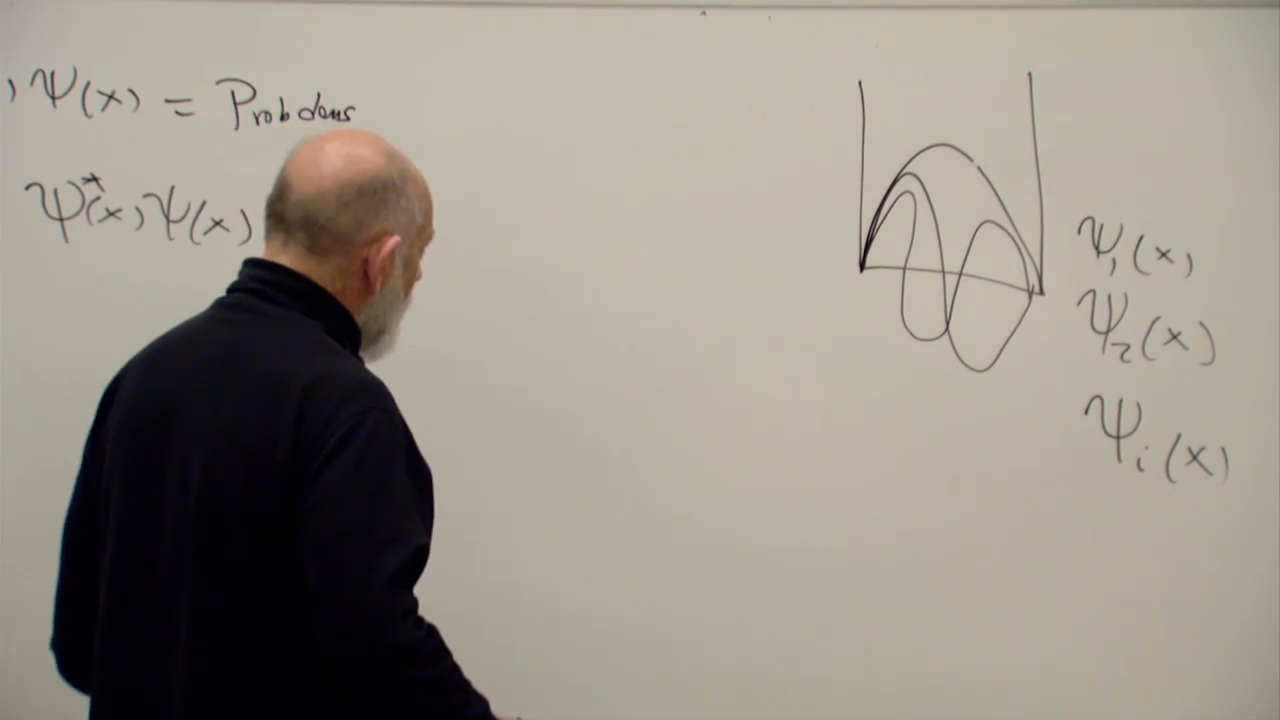
\includegraphics[width=0.94\linewidth]{lecture_07_frame_01.png}
\caption{Les modes de la boîte au tableau pendant le cours. À gauche, on distingue encore la densité de Born et la normalisation à une particule ; à droite, le puits montre \(\psi_1(x)\), \(\psi_2(x)\) et l’étiquette générale \(\psi_i(x)\).}
\lectureframe{00:08:25}
\end{figure}

On peut dégager la même structure modale de ce qui masque le tableau pendant le cours :
\begin{figure}[htbp]
\centering
\begin{tikzpicture}[x=1cm,y=1cm]
  \draw[thick] (0,0) -- (0,4.0);
  \draw[thick] (7,0) -- (7,4.0);
  \draw[gray!55] (0,2.85) -- (7,2.85);
  \draw[gray!55] (0,1.35) -- (7,1.35);
  \draw[blue!75!black,thick,domain=0:7,samples=120]
    plot (\x,{2.85+0.62*sin(180*\x/7)});
  \draw[teal!70!black,thick,domain=0:7,samples=120]
    plot (\x,{1.35+0.55*sin(360*\x/7)});
  \node[right] at (7.15,3.20) {$\psi_1(x)$};
  \node[right] at (7.15,1.70) {$\psi_2(x)$};
  \node at (3.5,0.38) {$\vdots\quad\psi_i(x)$};
\end{tikzpicture}
\caption{Reconstitution épurée du schéma qualitatif de la boîte. Les décalages verticaux servent uniquement à séparer les deux fonctions d’onde pour les représenter.}
\end{figure}

L’orthonormalité s’écrit
\begin{equation}
\int dx\,\psi_i^*(x)\psi_j(x)=\delta_{ij}.
\label{eq:l07-orthonormality}
\end{equation}
Si \(i=j\), l’état est normalisé et l’intégrale vaut un. Si \(i\ne j\), les deux états sont orthogonaux et l’intégrale s’annule.

La complétude est une affirmation tout aussi importante :
\begin{equation}
\sum_i |i\rangle\langle i|=\mathbf 1.
\label{eq:l07-resolution}
\end{equation}
Chaque \(|i\rangle\langle i|\) projette sur une direction de la base ; la somme sur la base complète est l’identité. Appliquée à un vecteur quelconque, elle décompose simplement ce vecteur en ses composantes, puis le reconstitue.

Insérons maintenant l’équation~\eqref{eq:l07-resolution} entre deux états de position :
\begin{align}
\langle y|x\rangle
&=\sum_i\langle y|i\rangle\langle i|x\rangle \\
&=\sum_i\psi_i(y)\psi_i^*(x) \\
&=\delta(y-x).
\label{eq:l07-position-completeness}
\end{align}
L’astérisque porte sur le facteur dont l’ordre dans le bra-ket est \(\langle i|x\rangle\). Inverser \(x\) et \(y\) donne une forme équivalente, complexe conjuguée. Ainsi, toute base complète orthonormée fournit une représentation de la fonction delta. Les sinus, les cosinus, les fonctions d’onde de l’oscillateur et les fonctions propres d’énergie remplissent tous ce rôle.

\begin{classroomqa}
\lecturetimestamp{00:13:43}
\audiencequestion{La deuxième fonction d’onde de la somme de complétude doit-elle porter le complexe conjugué ?}
\lecturerresponse{Oui. Dans l’ordre \(\langle y|i\rangle\langle i|x\rangle\), les facteurs sont \(\psi_i(y)\psi_i^*(x)\). Garder visible l’ordre du bra-ket évite de deviner ou de mal placer l’astérisque.}
\end{classroomqa}

Voilà les mathématiques à une particule dont nous aurons besoin. Changeons maintenant d’espace d’états.

\section{L’espace de Fock comme espace d’états élargi}

Pour plusieurs particules identiques, une base commode indique combien de particules occupent chaque mode à une particule :
\begin{equation}
|n_1,n_2,n_3,\ldots\rangle.
\label{eq:l07-fock-basis}
\end{equation}
L’entier \(n_i\) est le nombre d’occupation du mode \(i\). Ce ket n’est pas un état à une particule écrit dans une notation plus sophistiquée. Il appartient à un espace de Hilbert plus vaste qui contient le secteur à zéro particule, tous les états à une particule, tous les états à deux particules, et ainsi de suite. Cet espace élargi s’appelle l’espace de Fock.

Pour modifier les occupations, introduisons, pour chaque mode, un opérateur de création et un opérateur d’annihilation :
\begin{equation}
a_i^\dagger,\qquad a_i.
\end{equation}
Le premier ajoute une particule au mode \(i\), tandis que le second en enlève une. À ce stade, le langage de l’oscillateur harmonique sert d’outil de comptabilité : il n’est pas nécessaire qu’un ressort oscille littéralement. L’algèbre de l’oscillateur fournit exactement les outils nécessaires pour augmenter ou diminuer les nombres d’occupation.

L’opérateur nombre du mode est
\begin{equation}
\begin{aligned}
N_i&=a_i^\dagger a_i,\\
N_i|n_1,\ldots,n_i,\ldots\rangle
&=n_i|n_1,\ldots,n_i,\ldots\rangle.
\end{aligned}
\end{equation}
Le vide est
\begin{equation}
|0\rangle\equiv|0,0,0,\ldots\rangle,
\qquad
a_i|0\rangle=0
\quad\text{for every }i.
\label{eq:l07-vacuum}
\end{equation}
Un état à une particule dans le mode \(i\) est donc
\begin{equation}
|i\rangle=a_i^\dagger|0\rangle.
\label{eq:l07-mode-created}
\end{equation}
Le même symbole \(|i\rangle\) peut désormais désigner soit un vecteur de base à une particule, soit ce vecteur intégré au secteur à une particule de l’espace de Fock. Cette intégration est donnée par l’équation~\eqref{eq:l07-mode-created} ; le contexte indique l’espace considéré.

\section{Réunir les modes dans un champ}

Définissons les champs d’annihilation et de création par
\begin{equation}
\Psi(x)=\sum_i \psi_i(x)a_i,
\qquad
\Psi^\dagger(x)=\sum_i \psi_i^*(x)a_i^\dagger.
\label{eq:l07-field-expansion}
\end{equation}
La majuscule est importante. Les fonctions \(\psi_i(x)\) minuscules sont des nombres complexes ; la majuscule \(\Psi(x)\) désigne un opérateur sur l’espace de Fock. En chaque point de l’espace \(x\), l’équation~\eqref{eq:l07-field-expansion} donne une combinaison linéaire différente des opérateurs de mode. C’est cela qu’on entend par fonction opératorielle de la position.

Pour des particules libres, les fonctions de mode peuvent être des ondes planes \(e^{ikx}\). L’équation~\eqref{eq:l07-field-expansion} est alors un développement de Fourier, à ceci près que ses coefficients de Fourier sont des opérateurs plutôt que des nombres. L’ancienne terminologie appelle les nombres complexes ordinaires des nombres \(c\) et les opérateurs quantiques des nombres \(q\). Les fonctions de mode sont des nombres \(c\) et commutent avec tout ; les opérateurs \(a_i\) et \(a_i^\dagger\) portent le caractère opératoriel.

Ni \(\Psi\) ni \(\Psi^\dagger\) n’est hermitien. Ils sont adjoints l’un de l’autre. Les deux combinaisons
\begin{equation}
\Psi+\Psi^\dagger,
\qquad
i(\Psi^\dagger-\Psi)
\label{eq:l07-hermitian-combinations}
\end{equation}
sont hermitiennes et peuvent représenter des observables. Pour l’instant, toutefois, les champs sont surtout utiles comme outils pour créer, annihiler et compter des particules localement.

\begin{classroomqa}
\lecturetimestamp{00:21:05}
\audiencequestion{Que signifie le fait qu’un opérateur dépende de \(x\) ?}
\lecturerresponse{Cela signifie que chaque valeur de \(x\) sélectionne un opérateur différent. La dépendance spatiale est portée par les fonctions de mode ordinaires, tandis que chaque combinaison linéaire obtenue agit sur le même espace de Fock.}
\end{classroomqa}

\section{Ce que fait le champ de création}

Une définition devient utile lorsqu’on demande ce qu’elle fait. Partons d’un état propre de position dans le secteur à une particule et insérons la résolution de l’identité :
\begin{align}
|x\rangle
&=\sum_i |i\rangle\langle i|x\rangle \\
&=\sum_i a_i^\dagger|0\rangle\,\psi_i^*(x) \\
&=\Psi^\dagger(x)|0\rangle.
\label{eq:l07-local-creation}
\end{align}
Ainsi, \(a_i^\dagger\) crée une particule dans le mode bien défini \(i\), tandis que \(\Psi^\dagger(x)\) crée une particule localisée en \(x\). Dans la base de position idéalisée, cette localisation est au sens des distributions ; une préparation physique utiliserait un paquet d’ondes étroit, mais le sens algébrique est le même.

\begin{classroomqa}
\lecturetimestamp{00:24:48}
\audiencequestion{\(\sum_i|i\rangle\langle i|\) est-il un projecteur ?}
\lecturerresponse{Chaque terme est un projecteur sur un état de base. La somme complète est l’identité elle-même et s’appelle une résolution de l’identité. Son insertion ne modifie pas l’état, mais rend visibles ses composantes dans la base choisie.}
\end{classroomqa}

L’équation~\eqref{eq:l07-local-creation} donne la première interprétation directe du champ en termes de particules. Nous n’avons pas simplement accolé une étiquette spatiale à un opérateur abstrait. Nous avons construit l’opération qui crée une particule en ce point de l’espace.

\begin{classroomqa}
\lecturetimestamp{00:28:20}
\audiencequestion{Le champ de création dans l’espace des positions doit-il porter un astérisque ou une dague ?}
\lecturerresponse{Pour l’adjoint d’un opérateur, utilisez une dague. Les astérisques désignent le complexe conjugué des fonctions d’onde ordinaires \(\psi_i(x)\) ; les dagues se placent sur \(a_i^\dagger\) et \(\Psi^\dagger(x)\).}
\end{classroomqa}

\begin{classroomqa}
\lecturetimestamp{00:28:36}
\audiencequestion{Peut-on déplacer les opérateurs de création de part et d’autre des fonctions d’onde dans le développement en modes ?}
\lecturerresponse{Oui. Les \(\psi_i(x)\) sont des nombres \(c\) et commutent donc avec tout opérateur. Il faut seulement faire attention lorsqu’on change l’ordre d’opérateurs qui ne commutent pas, tels que \(a_i\) et \(a_j^\dagger\).}
\end{classroomqa}

\section{De la densité de probabilité à la densité de particules}

Jouons maintenant avec le champ. L’expression qui vient naturellement est
\begin{equation}
\int dx\,\Psi^\dagger(x)\Psi(x).
\end{equation}
Elle ressemble à l’intégrale de normalisation à une particule, mais ses facteurs sont désormais des opérateurs. Insérons les développements en modes sans en modifier l’ordre :
\begin{align}
\int dx\,\Psi^\dagger(x)\Psi(x)
&=\int dx
\left(\sum_i a_i^\dagger\psi_i^*(x)\right)\\
&\qquad\times\left(\sum_j a_j\psi_j(x)\right) \\
&=\sum_{i,j}a_i^\dagger a_j
\int dx\,\psi_i^*(x)\psi_j(x) \\
&=\sum_{i,j}a_i^\dagger a_j\,\delta_{ij} \\
&=\sum_i a_i^\dagger a_i.
\label{eq:l07-number-derivation}
\end{align}
L’opérateur nombre total est donc
\begin{equation}
N=\sum_i N_i
=\int dx\,\Psi^\dagger(x)\Psi(x).
\label{eq:l07-total-number}
\end{equation}
Pour les états considérés, les occupations des excitations d’énergie finie décroissent à haute énergie de mode, si bien que ce total est en général fini, même si l’ensemble des modes possibles est infini.

L’intégrande est l’opérateur de densité locale de particules :
\begin{equation}
n(x)=\Psi^\dagger(x)\Psi(x).
\label{eq:l07-density}
\end{equation}
À proprement parler, on ne mesure pas la densité en un point mathématique. Pour une petite région \(R\), on mesure
\begin{equation}
N_R=\int_R dx\,n(x),
\label{eq:l07-regional-number}
\end{equation}
le nombre de particules dans cette région. Comme toute observable quantique, \(N_R\) n’a pas nécessairement de valeur déterminée dans un état arbitraire. Des préparations répétées peuvent donner des résultats différents.

\begin{classroomqa}
\lecturetimestamp{00:36:27}
\audiencequestion{\(\Psi^\dagger(x)\Psi(x)\) est-elle la densité de probabilité à plusieurs particules ?}
\lecturerresponse{Son interprétation directe est celle d’une densité de particules. Une amplitude de probabilité à plusieurs particules dépend généralement de toutes les coordonnées des particules. La forme bilinéaire locale, elle, compte les particules dans une petite région lorsqu’on l’intègre sur cette région.}
\end{classroomqa}

\begin{classroomqa}
\lecturetimestamp{00:38:28}
\audiencequestion{Les opérateurs \(a_i\) et \(a_i^\dagger\) agissent-ils uniquement sur les vecteurs d’état, et pas sur les fonctions d’onde à une particule ?}
\lecturerresponse{Oui. Ils agissent sur les états de l’espace de Fock, tels que \(|n_1,n_2,\ldots\rangle\). Les fonctions de mode à une particule qui les multiplient sont des nombres ordinaires, et ces opérateurs d’échelle n’agissent pas sur elles.}
\end{classroomqa}

Les kets d’occupation forment une base, mais ne constituent pas l’état le plus général. On peut les superposer, y compris de façon à répartir différemment un même nombre total de particules entre les modes. Pour des espèces neutres comme les photons, on peut aussi superposer des secteurs ayant des nombres totaux de particules différents. L’opérateur de l’équation~\eqref{eq:l07-regional-number} conserve la même signification opérationnelle dans chacun de ces états.

\begin{classroomqa}
\lecturetimestamp{00:40:01}
\audiencequestion{Si l’on divise la densité de particules par le nombre total, obtient-on la densité de probabilité de trouver une particule en \(x\) ?}
\lecturerresponse{Dans une situation à \(N\) fixé et à grand nombre de particules, \(N_R/N\) est une fréquence relative et suit généralement de très près une probabilité à une particule. Il ne s’agit pas d’une identité opératorielle qui ferait d’un résultat de mesure une probabilité. Le nombre mesuré fluctue, typiquement d’une quantité de l’ordre de \(\sqrt N\) dans un modèle de particules indépendantes, et un résultat exceptionnel peut s’écarter fortement de la probabilité, même s’il est peu probable.}
\end{classroomqa}

\begin{classroomqa}
\lecturetimestamp{00:42:25}
\audiencequestion{Qu’advient-il de la conservation de la charge dans une superposition d’un état à un électron et d’un état sans électron ?}
\lecturerresponse{Ce n’est pas le type de superposition utilisé dans un secteur fermé de charge électrique fixée. On peut superposer différentes répartitions qui ont la même charge totale. Les photons n’ayant pas de charge électrique, les secteurs de nombre de photons différents ne posent pas ce problème. Le nombre d’électrons et de positrons peut aussi varier simultanément tout en conservant la charge nette.}
\end{classroomqa}

\section{Énergie de particules indépendantes}

L’énergie est la prochaine observable. Commençons par nous limiter à des particules qui n’interagissent pas entre elles. Cette approximation est souvent bonne dans un système dilué. Même les photons interagissent en principe par des processus d’ordre supérieur, mais le rayonnement ordinaire en laboratoire est assez dilué pour que la description par des particules indépendantes soit excellente.

Notons \(\omega_i\) l’énergie d’une particule dans le mode \(i\), avec \(\hbar=1\). Un mode désigne un état à une particule. L’hamiltonien total est alors
\begin{equation}
H=\sum_i\omega_i N_i
=\sum_i\omega_i a_i^\dagger a_i.
\label{eq:l07-mode-hamiltonian}
\end{equation}
Chaque mode occupé contribue son énergie à une particule une fois par particule.

\begin{classroomqa}
\lecturetimestamp{00:48:16}
\audiencequestion{\(\omega_i\) est-elle une fonction de la position ?}
\lecturerresponse{Non. C’est la valeur propre d’énergie associée au mode \(i\). La fonction \(\psi_i(x)\) dépend de la position ; \(\omega_i\) dépend du niveau d’énergie sélectionné.}
\end{classroomqa}

Les valeurs \(\omega_i\) sont déterminées par l’équation de Schrödinger indépendante du temps à une particule. Définissons
\begin{equation}
h=-\frac{\nabla^2}{2m}+V(x).
\label{eq:l07-one-particle-h}
\end{equation}
On a alors
\begin{equation}
h\psi_i(x)=\omega_i\psi_i(x).
\label{eq:l07-schrodinger-eigenvalue}
\end{equation}
En une dimension, l’opérateur quantité de mouvement est \(p=-i\partial_x\), et \(p^2/(2m)\) devient \(-\partial_x^2/(2m)\). En trois dimensions, les trois dérivées secondes se combinent en \(-\nabla^2/(2m)\).

\begin{figure}[htbp]
\centering
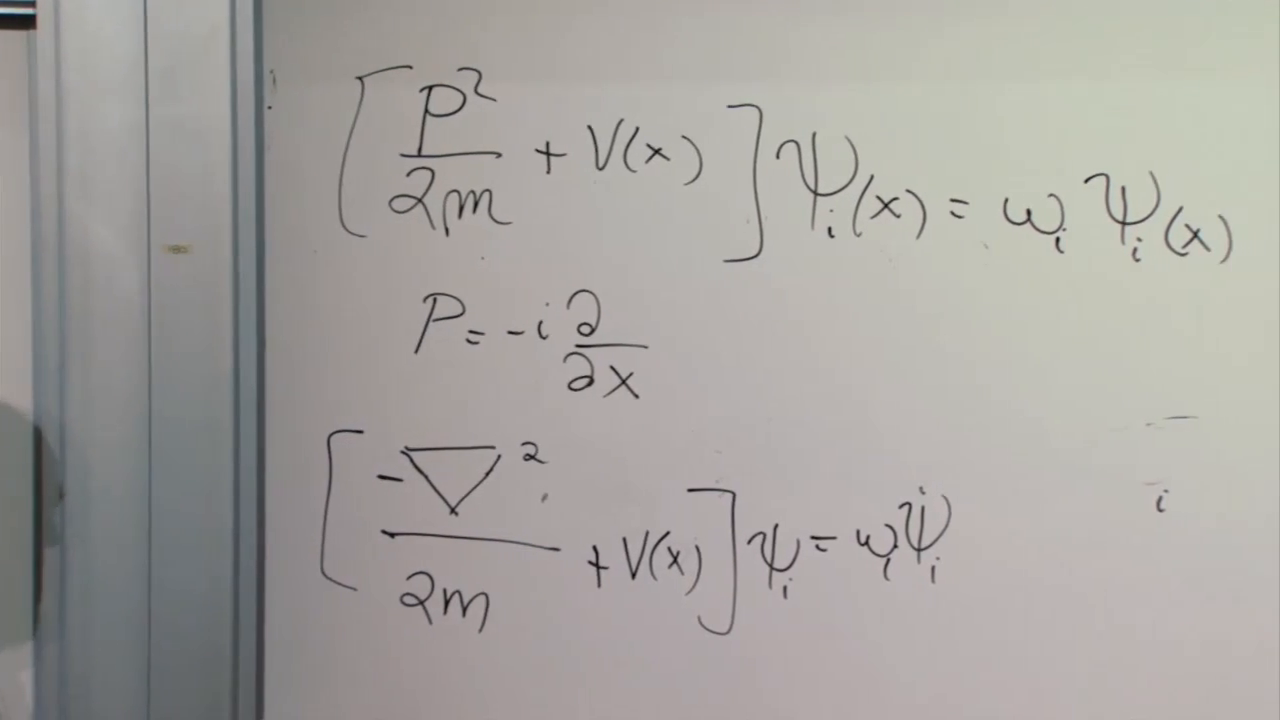
\includegraphics[width=0.94\linewidth]{lecture_07_frame_02.png}
\caption{Passage au tableau de \(p^2/(2m)+V(x)\) à la forme différentielle de l’équation aux valeurs propres de Schrödinger à une particule. L’équation~\eqref{eq:l07-schrodinger-eigenvalue} en est une reconstitution épurée.}
\lectureframe{00:54:10}
\end{figure}

Pour une fonction d’onde à une particule normalisée quelconque, la valeur moyenne usuelle est
\begin{equation}
\langle h\rangle_\psi
=\int dx\,\psi^*(x)h\psi(x).
\label{eq:l07-one-particle-energy-expectation}
\end{equation}
On peut conjecturer la formule à plusieurs particules en remplaçant la fonction d’onde minuscule par le champ à valeurs opératorielles. Ce n’est pas encore une démonstration, mais la conjecture dont nous allons vérifier la validité :
\begin{equation}
H=\int dx\,\Psi^\dagger(x)h\Psi(x).
\label{eq:l07-field-hamiltonian}
\end{equation}

\section{Écrire d’abord le résultat, puis le démontrer}

Insérons l’équation~\eqref{eq:l07-field-expansion} dans l’hamiltonien proposé :
\begin{align}
\int dx\,\Psi^\dagger h\Psi
&=\int dx
\left(\sum_i a_i^\dagger\psi_i^*(x)\right)
h\left(\sum_j a_j\psi_j(x)\right) \\
&=\sum_{i,j}a_i^\dagger a_j
\int dx\,\psi_i^*(x)h\psi_j(x).
\label{eq:l07-h-expanded}
\end{align}
L’opérateur différentiel \(h\) agit sur la fonction d’onde \(\psi_j(x)\) qui dépend de \(x\), et non sur l’opérateur de mode \(a_j\). D’après l’équation de Schrödinger,
\begin{equation}
h\psi_j(x)=\omega_j\psi_j(x).
\end{equation}
Il s’ensuit que
\begin{align}
\int dx\,\Psi^\dagger h\Psi
&=\sum_{i,j}a_i^\dagger a_j\omega_j
\int dx\,\psi_i^*(x)\psi_j(x) \\
&=\sum_{i,j}a_i^\dagger a_j\omega_j\delta_{ij} \\
&=\sum_j\omega_j a_j^\dagger a_j.
\label{eq:l07-h-proof}
\end{align}
C’est précisément l’équation~\eqref{eq:l07-mode-hamiltonian}. L’expression locale du champ et la somme des énergies de toutes les particules désignent le même opérateur.

\begin{figure}[htbp]
\centering
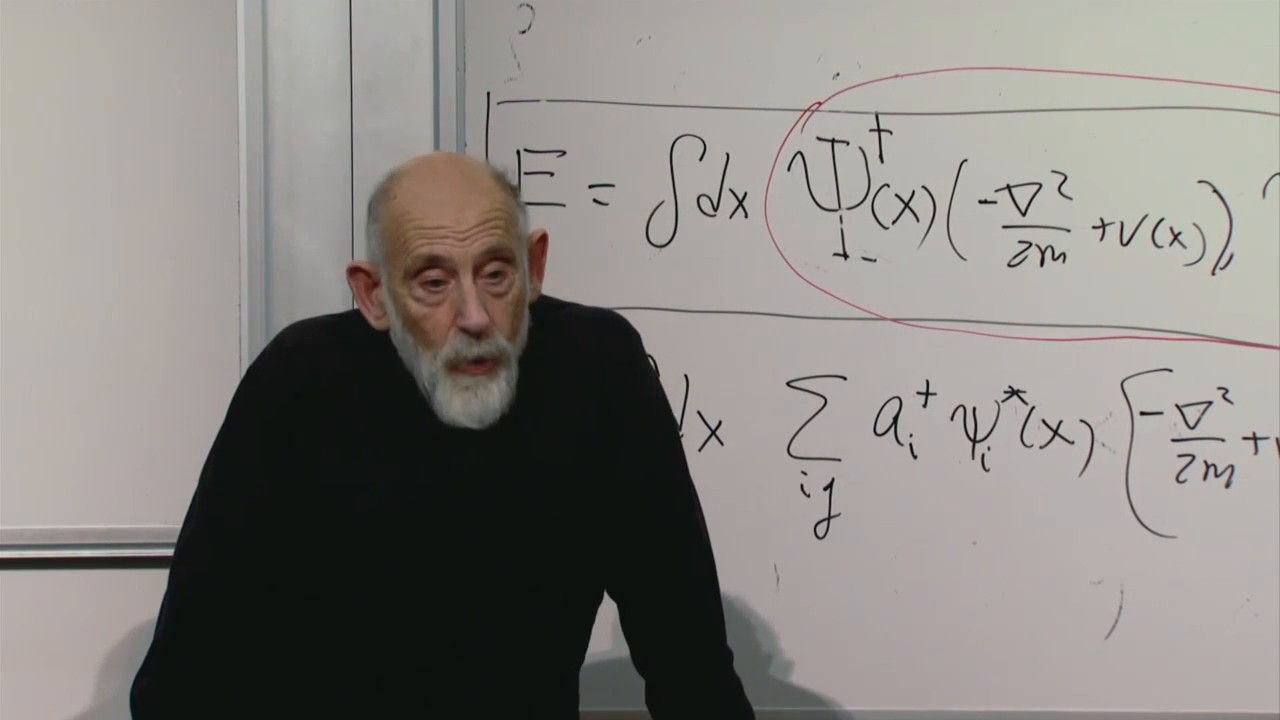
\includegraphics[width=0.94\linewidth]{lecture_07_frame_03.png}
\caption{L’hamiltonien du champ mis en évidence au tableau, avec le début de la démonstration par développement en modes en dessous. L’image prise pendant le cours est conservée comme élément de preuve ; les équations~\eqref{eq:l07-field-hamiltonian}--\eqref{eq:l07-h-proof} rétablissent tout le calcul.}
\lectureframe{01:05:34}
\end{figure}

Dans cette démonstration, aucun opérateur de création n’a été commuté avec un opérateur d’annihilation. L’ordre \(a_i^\dagger a_j\) est conservé du début à la fin. Seules les fonctions d’onde, nombres \(c\), et leurs valeurs propres sont déplacées librement.

\section{Pourquoi s’agit-il d’un champ ?}

Pourquoi appeler \(\Psi(x)\) un champ ? Parce qu’il s’agit d’une grandeur à valeurs opératorielles définie en chaque point de l’espace, et que les combinaisons hermitiennes ou les formes bilinéaires qu’on en construit sont des observables locales. La densité \(n(x)\) et l’expression locale de l’énergie présentée plus loin en sont deux exemples. Le mot ne cache aucun autre critère mathématique.

Ce champ n’est pas le champ électromagnétique. Il décrit l’espèce non relativiste dont proviennent les modes et l’hamiltonien à une particule \(p^2/(2m)+V\) : par exemple des atomes lents, des neutrons, des protons ou des électrons. Ces particules sont les quanta de leur champ respectif, au même sens structurel que les photons sont les quanta du champ électromagnétique.

\begin{classroomqa}
\lecturetimestamp{01:02:45}
\audiencequestion{À quel moment un champ intervient-il dans le passage du système à plusieurs particules à la formule ci-dessus ?}
\lecturerresponse{Il intervient dans l’équation~\eqref{eq:l07-field-expansion} : \(\Psi(x)\) est un opérateur en chaque point de l’espace. Les dérivations qui suivent montrent que ses produits locaux mesurent les densités de particules et d’énergie. Dépendance en position et contenu opératoriel : voilà précisément la structure de champ que nous construisons.}
\end{classroomqa}

\section{Densité locale d’énergie}

L’équation~\eqref{eq:l07-field-hamiltonian} exprime l’énergie totale comme une intégrale sur l’espace :
\begin{equation}
\begin{aligned}
H&=\int dx\,\mathcal H(x),\\
\mathcal H(x)
&=-\frac{1}{2m}\Psi^\dagger(x)\nabla^2\Psi(x)\\
&\quad+V(x)\Psi^\dagger(x)\Psi(x).
\end{aligned}
\label{eq:l07-hamiltonian-density}
\end{equation}
L’intégrande constitue une densité locale d’énergie naturelle pour cet hamiltonien. Sa forme locale n’est pas unique. Par exemple, une intégration par parties remplace le terme cinétique par
\begin{equation}
\mathcal H_{\rm kin}(x)
=\frac{1}{2m}\nabla\Psi^\dagger(x)\mathbin{\cdot}\nabla\Psi(x)
\label{eq:l07-kinetic-density}
\end{equation}
à un terme de bord près. Les deux expressions donnent le même hamiltonien total sous les conditions aux limites habituelles. C’est la petite ambiguïté mentionnée dans le cours.

\begin{classroomqa}
\lecturetimestamp{01:05:57}
\audiencequestion{Faut-il intégrer la densité d’énergie sur tout l’espace ?}
\lecturerresponse{L’intégration sur tout l’espace donne l’énergie totale. L’intégration sur une région plus petite donne l’énergie attribuée à cette région, sous réserve de l’ambiguïté habituelle dans le choix d’une densité locale dont l’intégrale sur tout l’espace donne le même hamiltonien.}
\end{classroomqa}

\begin{classroomqa}
\lecturetimestamp{01:06:25}
\audiencequestion{En quoi la majuscule \(N_i\) de la formule de l’énergie diffère-t-elle de la minuscule \(n_i\) ?}
\lecturerresponse{\(N_i=a_i^\dagger a_i\) est un opérateur. L’entier \(n_i\) est l’une de ses valeurs propres sur un état de nombre d’occupation. Les opérateurs agissent sur des états ; leurs valeurs propres sont des nombres ordinaires.}
\end{classroomqa}

\begin{classroomqa}
\lecturetimestamp{01:06:46}
\audiencequestion{Peut-on écrire l’hamiltonien du champ lui-même sous forme de bra ou de ket dans la notation de Dirac ?}
\lecturerresponse{Non. Les bras et les kets désignent des vecteurs d’état et leurs éléments duaux. Le champ et l’hamiltonien sont des opérateurs agissant sur ces états. Une valeur moyenne telle que \(\langle\Phi|H|\Phi\rangle\) fait intervenir les deux types d’objets, qu’il ne faut pas confondre.}
\end{classroomqa}

\section{Retrouver une particule et approcher un champ classique}

Le formalisme élargi contient la mécanique quantique ordinaire à une particule. Restreignons l’espace de Fock aux états qui satisfont à
\begin{equation}
N|\Phi\rangle=|\Phi\rangle.
\end{equation}
Dans ce secteur, la construction du champ reproduit tous les états à une particule et toutes les prédictions à une particule. Nous n’avons pas remplacé l’ancienne théorie ; nous l’avons intégrée dans un espace qui permet aussi de décrire zéro, deux ou un nombre quelconque de particules.

À l’autre extrême, un mode occupé par un très grand nombre de bosons peut se comporter approximativement comme une onde classique. Dans des états cohérents ou semi-classiques appropriés, la valeur moyenne
\begin{equation}
\Phi_{\rm cl}(x,t)=\langle\Psi(x,t)\rangle
\end{equation}
satisfait l’équation d’allure classique
\begin{equation}
i\partial_t\Phi_{\rm cl}(x,t)
=\left(-\frac{\nabla^2}{2m}+V(x)\right)\Phi_{\rm cl}(x,t)
\label{eq:l07-classical-schrodinger}
\end{equation}
pour la théorie libre non relativiste. Le cours énonce ce lien sans le démontrer. Il fait le pont entre un ensemble de quanta et un champ ondulatoire : les grandes occupations réduisent les fluctuations relatives et font que certaines valeurs moyennes se comportent classiquement.

Le formalisme relève donc à la fois de la comptabilité et de la physique. Il organise tous les secteurs de nombre de particules, tout en décrivant l’interférence, l’intrication et l’émergence d’ondes classiques à partir de particules quantiques.

\begin{classroomqa}
\lecturetimestamp{01:10:43}
\audiencequestion{Pourquoi peut-on manipuler les opérateurs de création et d’annihilation dans l’intégrale presque comme des nombres ordinaires ?}
\lecturerresponse{On ne les a jamais permutés l’un avec l’autre. Les fonctions de mode ordinaires commutent avec eux, et les dérivées agissent uniquement sur ces fonctions. Faire passer un opérateur d’annihilation à travers un opérateur de création nécessiterait d’utiliser le commutateur et pourrait ajouter un terme ; aucune étape de la démonstration n’effectue cette permutation.}
\end{classroomqa}

\section{Parenthèse sur la notation de Dirac}

Une partie de la confusion est historique. Une fonction d’onde à une particule satisfait une équation d’onde et ressemble superficiellement à un champ classique, tout en étant une amplitude de probabilité. Les débuts de la théorie quantique ont dû dissocier ces rôles, puis expliquer comment les champs ondulatoires réellement mesurables, comme l’électromagnétisme, sont constitués de quanta. L’espace de Fock et les champs à valeurs opératorielles résolvent ce conflit apparent.

La notation de Dirac rend cette distinction particulièrement concise. Un ket appartient à un espace vectoriel, un bra à son dual, et leur juxtaposition forme un produit scalaire. La résolution
\begin{equation}
\sum_i|i\rangle\langle i|=\mathbf 1
\end{equation}
devient alors presque limpide. Le cours l’illustre par une anecdote tirée d’un enseignement de mécanique quantique à des mathématiciens : le contenu mathématique leur était déjà familier, mais la notation rendait les manipulations usuelles si transparentes que la structure semblait nouvelle. L’idée n’est pas qu’une discipline ignorait le concept. C’est qu’une notation bien choisie rend difficile la confusion entre les opérations autorisées.

Cette leçon est importante ici. Il existe maintenant plusieurs opérateurs distincts :
\begin{itemize}
\item \(h\) agit sur les fonctions d’onde à une particule comme un opérateur différentiel ;
\item \(a_i\) et \(a_i^\dagger\) agissent sur les états de nombre d’occupation dans l’espace de Fock ;
\item \(\Psi(x)\), \(\Psi^\dagger(x)\), \(N\) et \(H\) agissent eux aussi sur l’espace de Fock.
\end{itemize}
Le développement de l’équation~\eqref{eq:l07-field-expansion} relie les deux premiers cadres sans les confondre.

\begin{classroomqa}
\lecturetimestamp{01:18:16}
\audiencequestion{Les champs ne sont-ils qu’un formalisme pour décrire des ensembles de particules ?}
\lecturerresponse{C’est un formalisme, mais il n’est pas vide de contenu. Ses observables locales sont mesurables, et les particules sont des objets quantiques qui présentent interférence et intrication, et non des boulettes classiques. Les opérateurs de champ encodent précisément ces propriétés collectives mesurables.}
\end{classroomqa}

\section{Prudence relativiste et aparté sur l’électromagnétisme}

La construction présentée jusqu’ici est non relativiste. En physique relativiste, la quantité de mouvement reste un bon label des particules, mais la localisation précise de leur position est beaucoup plus délicate. Par conséquent, une densité locale de nombre de photons n’est généralement pas une notion aussi nette que \(n(x)\) dans le cas non relativiste. La densité d’énergie reste bien définie et constitue l’observable locale la plus sûre.

Le cours propose une analogie électromagnétique utile, explicitement heuristique. Regroupons les champs électrique et magnétique dans le vecteur complexe
\begin{equation}
\mathbf F=\mathbf E+i\mathbf B,
\qquad
\mathbf F^*=\mathbf E-i\mathbf B.
\label{eq:l07-riemann-silberstein}
\end{equation}
On a alors
\begin{equation}
\mathbf F^*\mathbin{\cdot}\mathbf F
=\mathbf E^2+\mathbf B^2,
\label{eq:l07-em-density}
\end{equation}
qui est proportionnel à la densité d’énergie électromagnétique dans les unités conventionnelles. Il ne s’agit pas littéralement d’une densité de probabilité des photons. Il vaut mieux y voir une variable de champ compacte dont le carré du module mesure la densité d’énergie, ou, de manière informelle, une densité de photons pondérée par leur énergie.

\begin{classroomqa}
\lecturetimestamp{01:19:10}
\audiencequestion{Peut-on identifier la densité de photons à l’intensité du champ électrique ?}
\lecturerresponse{Seulement de façon qualitative et avec prudence. Pour des photons relativistes, le nombre local de particules n’est pas la notion à privilégier. L’affirmation robuste est que \(E^2+B^2\) est proportionnel à la densité d’énergie et que la combinaison complexe \(\mathbf E+i\mathbf B\) regroupe les équations de Maxwell sous une forme analogue à celle de Schrödinger.}
\end{classroomqa}

\begin{classroomqa}
\lecturetimestamp{01:20:09}
\audiencequestion{Pourquoi une particule relativiste peut-elle avoir une quantité de mouvement bien définie alors que sa position pose problème ?}
\lecturerresponse{La quantité de mouvement caractérise sans ambiguïté les représentations relativistes à une particule, tandis qu’une localisation stricte entre en conflit avec la création de particules et la description par les champs relativistes. Ce cours ne développe pas cette théorie ; cet avertissement marque la limite de l’interprétation non relativiste de la densité présentée ici.}
\end{classroomqa}

\section{Ordre des opérateurs et constante d’énergie du fondamental}

On ne peut pas modifier l’ordre des opérateurs à la légère. Pour les modes bosoniques,
\begin{equation}
a_i a_i^\dagger=a_i^\dagger a_i+1.
\end{equation}
Par conséquent, remplacer l’ordre normal \(\Psi^\dagger h\Psi\) par l’ordre inversé \((h\Psi)\Psi^\dagger\), ou par la forme correspondante correctement intégrée, ajoute la contribution du commutateur. Dans une base de modes, il s’agit d’une somme additive d’un quantum d’énergie par mode. C’est la constante d’énergie du fondamental, ou énergie du point zéro ; dans un continuum, elle nécessite une régularisation. Le cours n’examine pas cette question ici ; il signale simplement que les deux ordres ne sont pas équivalents.

\begin{classroomqa}
\lecturetimestamp{01:22:04}
\audiencequestion{Que se passe-t-il si \(\Psi\) et \(\Psi^\dagger\) sont intervertis dans l’Hamiltonien ?}
\lecturerresponse{Leur commutateur doit être pris en compte. Inverser leur ordre ajoute donc une contribution à l’état fondamental indépendante de l’état considéré, au lieu de redonner la même expression. L’Hamiltonien affiché est écrit en ordre normal, \(\Psi^\dagger h\Psi\).}
\end{classroomqa}

\section{La quantité de mouvement, dernier test}

Les dernières minutes reprennent une fois de plus la même promotion. Pour une particule,
\begin{equation}
\langle p\rangle_\psi
=\int dx\,\psi^*(x)\left(-i\partial_x\right)\psi(x).
\label{eq:l07-one-particle-momentum}
\end{equation}
En remplaçant la fonction d’onde par le champ, on obtient l’opérateur de quantité de mouvement totale
\begin{equation}
P=\int dx\,\Psi^\dagger(x)\left(-i\partial_x\right)\Psi(x),
\label{eq:l07-field-momentum}
\end{equation}
ou, en trois dimensions,
\begin{equation}
\mathbf P=\int d^3x\,\Psi^\dagger(\mathbf x)
\left(-i\boldsymbol\nabla\right)\Psi(\mathbf x).
\end{equation}
Les champs portent une quantité de mouvement. Un laser suffisamment puissant transfère de la quantité de mouvement à un mur et exerce une force ; dans la description quantique, la quantité de mouvement du champ est la somme des quantités de mouvement des photons.

L’équation~\eqref{eq:l07-field-momentum} est un opérateur, et non une valeur moyenne. À partir d’un état de l’espace de Fock \(|\Phi\rangle\), on peut alors calculer
\begin{equation}
\langle P\rangle_\Phi=\langle\Phi|P|\Phi\rangle.
\end{equation}
Il faut à la fois un opérateur et un état pour former une valeur moyenne. Confondre l’observable avec sa valeur moyenne effacerait précisément la distinction que le cours a établi.

\begin{classroomqa}
\lecturetimestamp{01:26:02}
\audiencequestion{La quantité de mouvement du champ affichée est-elle déjà la quantité de mouvement moyenne ?}
\lecturerresponse{Non. C’est l’opérateur hermitien qui représente l’observable. Il faut fournir un état et placer l’opérateur entre le bra et le ket de cet état pour obtenir une valeur moyenne ; une mesure peut néanmoins fluctuer autour de cette moyenne.}
\end{classroomqa}

C’est le point d’arrêt naturel. À partir des particules, nous avons construit des champs locaux de création et d’annihilation, nous nous en sommes servis pour compter les particules et avons réécrit la somme des énergies et des quantités de mouvement des particules comme des opérateurs de champ. L’étape suivante ne consiste pas à changer encore de notation. Il s’agit de faire représenter des processus physiques par les opérateurs de champ : la désintégration des particules, leur diffusion et les transformations d’une espèce en une autre.
\chapter{Mélange, oscillations, moments dipolaires électriques et opérateurs de champ}

Commençons par nous écarter un peu du sujet annoncé et poser une question sur les neutrinos. Des indices montrent que les neutrinos ont une masse et que leurs types se mélangent. Si leurs masses ne sont pas toutes identiques, comment un type peut-il se transformer en un autre sans violer la conservation de l’énergie ?

Cette question nous mène à un phénomène récurrent en mécanique quantique : les états dans lesquels un système est préparé ou détecté ne sont pas nécessairement ceux qui diagonalisent son hamiltonien. Un état d’énergie définie ne fait qu’acquérir une phase. En revanche, un état préparé comme superposition de plusieurs énergies évolue parce que ses composantes acquièrent des phases différentes. Cette distinction nous conduira du double puits aux oscillations des neutrinos et à la précession du spin. Après une parenthèse consacrée au moment dipolaire électrique de l’électron, nous reviendrons à la seconde quantification et retrouverons la même structure de Fourier position--impulsion au niveau des opérateurs.

\section{Le véritable enjeu : le mélange}

Les neutrinos n’ont pas nécessairement tous la même masse. Les états propres d’énergie ne se mélangent pas entre eux : chacun évolue indépendamment. Ce que nous appelons le \emph{type} ou la saveur d’un neutrino est lié à la façon dont il est produit et détecté ; un état de saveur peut être une combinaison linéaire d’états propres de masse et d’énergie. Schématiquement, \begin{equation}
|\text{type}\rangle = \sum_n c_n |E_n\rangle .
\end{equation}La bonne formulation n’est donc pas que les états propres d’énergie se transforment les uns en les autres, mais que les états appelés ``neutrino électronique'' ou ``neutrino muonique'' ne sont pas nécessairement eux-mêmes des états propres d’énergie.

\begin{classroomqa}\lecturetimestamp{00:00:09}\audiencequestion{Si les neutrinos ont des masses différentes, comment peuvent-ils se mélanger alors que l’énergie se conserve ?}\lecturerresponse{Les états propres de masse et d’énergie ne se transforment pas les uns en les autres. Les états de saveur électronique, muonique et tauique sont différentes combinaisons linéaires de ces états propres. Chaque composante de masse évolue avec sa propre phase, et l’interférence modifie les probabilités de saveur sans violer la conservation de l’énergie.}\end{classroomqa}

Cette structure se retrouve dans de nombreux exemples. Le plus parlant commence par une particule dans un double puits symétrique.

\section{Puits double symétrique et états approximativement localisés}

Considérons une particule dans un potentiel symétrique à double puits, avec une barrière élevée entre les deux minima. Si la hauteur de la barrière était infinie, les puits gauche et droit seraient complètement découplés. On pourrait résoudre le problème dans le puits de gauche comme si celui de droite n’existait pas, et réciproquement. Les fonctions d’onde approchées de l’état fondamental seraient alors un état localisé à gauche \(\psi_L\) et un état localisé à droite \(\psi_R\), tous deux d’énergie \(E\).

Dans chaque puits isolé, l’état fondamental possède les propriétés qualitatives habituelles : il est lisse, sans nœud, et se situe à l’énergie la plus basse compatible avec le confinement. Imaginons que la haute barrière centrale soit un mur de briques. La traiter comme infinie n’est qu’une approximation, mais elle nous fournit une paire utile d’états localisés pour commencer.

\begin{figure}\centering
\begin{adjustbox}{max width=\linewidth}\begin{tikzpicture}[x=0.8cm,y=0.8cm]
\begin{scope}[shift={(-5.8,0)}]
\draw (-4,2.7) .. controls (-3.35,1.2) and (-2.55,-0.45) .. (-2.0,-0.72)
      .. controls (-1.35,-0.95) and (-0.7,0.65) .. (0,2.05)
      .. controls (0.7,0.65) and (1.35,-0.95) .. (2.0,-0.72)
      .. controls (2.55,-0.45) and (3.35,1.2) .. (4,2.7);
\draw[dashed] (-4,-0.10) -- (4,-0.10);
\node at (-3.55,-0.48) {$E$};
\draw[line width=0.9pt] (-4,-0.02) .. controls (-3.2,-0.02) and (-2.7,0.30) .. (-2.15,0.95)
      .. controls (-1.55,1.30) and (-1.15,0.35) .. (-0.55,-0.06)
      .. controls (0.15,-0.14) and (0.9,-0.15) .. (4,-0.15);
\node at (-2.15,1.35) {$\psi_L$};
\end{scope}
\begin{scope}[shift={(5.8,0)}]
\draw (-4,2.7) .. controls (-3.35,1.2) and (-2.55,-0.45) .. (-2.0,-0.72)
      .. controls (-1.35,-0.95) and (-0.7,0.65) .. (0,2.05)
      .. controls (0.7,0.65) and (1.35,-0.95) .. (2.0,-0.72)
      .. controls (2.55,-0.45) and (3.35,1.2) .. (4,2.7);
\draw[dashed] (-4,-0.10) -- (4,-0.10);
\node at (-3.55,-0.48) {$E$};
\draw[line width=0.9pt] (-4,-0.02) .. controls (-3.2,-0.01) and (-2.7,0.30) .. (-2.15,0.95)
      .. controls (-1.6,1.28) and (-1.1,0.25) .. (-0.30,-0.08)
      .. controls (0.35,-0.12) and (0.85,-0.12) .. (1.35,0.35)
      .. controls (1.9,0.88) and (2.35,1.15) .. (2.85,0.55)
      .. controls (3.2,0.05) and (3.55,-0.12) .. (4,-0.15);
\end{scope}
\end{tikzpicture}\end{adjustbox}\caption{Redessin soigné des schémas d’ouverture au tableau. À gauche figure l’état d’essai unilatéral \(\psi_L\), obtenu en faisant comme si la barrière était effectivement infinie. À droite, la même fonction d’onde est prolongée symétriquement à travers la barrière, illustrant la faible fuite, non nulle, qui donnera finalement le véritable état fondamental pair.}\end{figure}

En mécanique quantique, toutefois, la barrière n’est pas réellement infinie. La fonction d’onde dans la région de la barrière n’est pas exactement nulle ; elle est seulement très petite. Toute l’histoire tient à cette infime fuite. C’est elle qui transforme l’approximation gauche-droite en un véritable problème de mélange.

\section{États propres de parité et dédoublement exponentiellement faible des niveaux}

Le tableau des états localisés est maintenant interrompu par un théorème : si le potentiel est symétrique, on peut choisir les fonctions propres exactes de l’énergie de sorte qu’elles soient soit symétriques, soit antisymétriques par réflexion.

\begin{theorem}Si \(V(x)=V(-x)\) en une dimension, les fonctions propres de l’hamiltonien peuvent être choisies de sorte à satisfaire l’une ou l’autre des relations suivantes : \[
\psi(x)=\psi(-x)
\qquad \text{or} \qquad
\psi(x)=-\psi(-x).
\]\end{theorem}

Voici maintenant la correction. Les états unilatéraux \(\psi_L\) et \(\psi_R\) ne sont ni symétriques ni antisymétriques ; ils ne peuvent donc pas être des états propres exacts de l’hamiltonien complet. Ce ne sont que de bons états approchés lorsque la barrière est élevée. Les véritables états propres sont les combinaisons symétrique et antisymétrique, \begin{align}
\psi_+ &= \frac{\psi_L+\psi_R}{\sqrt{2}},\\
\psi_- &= \frac{\psi_L-\psi_R}{\sqrt{2}}.
\end{align}En notant leurs énergies comme elles le seront au tableau, on a \begin{align}
H\psi_+ &= (E_1-\epsilon)\psi_+,\\
H\psi_- &= (E_1+\epsilon)\psi_-.
\end{align}L’écart total vaut donc \begin{equation}
\Delta E = (E_1+\epsilon)-(E_1-\epsilon)=2\epsilon .
\end{equation}

\begin{figure}[htbp]\centering
\includegraphics[width=0.92\linewidth]{lecture_08_frame_02.png}\caption{La fonction d’onde prolongée symétriquement dans le potentiel à double puits. Son amplitude sous la barrière est faible mais non nulle, ce qui est à l’origine de la séparation des niveaux.}\lectureframe{00:06:19}\end{figure}

\begin{figure}\centering
\begin{tikzpicture}[x=1cm,y=1cm]
\draw[->] (0,0) -- (0,3);
\node[left] at (0,2.8) {energy};
\draw (-0.35,1.60) -- (0.35,1.60);
\node[left] at (-0.45,1.60) {$\psi_L,\psi_R$};
\node at (1.7,1.60) {$\Longrightarrow$};
\draw (3.0,1.32) -- (3.75,1.32);
\draw (3.0,1.88) -- (3.75,1.88);
\draw[dashed] (2.8,1.60) -- (3.95,1.60);
\node[right] at (3.9,1.32) {$\psi_+,\ E_1-\epsilon$};
\node[right] at (3.9,1.88) {$\psi_-,\ E_1+\epsilon$};
\node[below] at (3.37,1.60) {$E_1$};
\end{tikzpicture}\caption{Schéma au tableau de la séparation par effet tunnel. Les états approchés gauche et droit sont presque dégénérés, mais les états propres exacts symétrique et antisymétrique sont séparés par une petite quantité \(2\epsilon\).}\end{figure}

L’ordre des niveaux porte en lui le point physique. L’état symétrique est légèrement plus bas en énergie, car il est plus lisse dans la région de la barrière ; le fait que la fonction d’onde puisse fuir et se prolonger symétriquement abaisse l’énergie d’une petite quantité. L’état antisymétrique est légèrement plus haut : en une dimension, le premier état excité possède un nœud, qui, dans ce problème symétrique, se trouve au milieu. Une courbure supplémentaire coûte de l’énergie cinétique.

L’effet est très faible, exponentiellement faible en fonction de la largeur et de la hauteur de la barrière. Il n’est pas nécessaire d’écrire ici une formule WKB explicite ; l’essentiel est que la séparation existe, mais qu’elle est minuscule. Rappelons aussi que le signe global d’une fonction d’onde n’a pas de signification physique. Remplacer \(\psi_-\) par \(-\psi_-\) ne change pas l’état.

\section{Évolution temporelle et oscillation gauche-droite}

Posons maintenant la question dynamique : que se passe-t-il si l’on place une particule dans le puits de gauche ? C’est l’étape décisive, car l’oscillation est la manifestation temporelle du même phénomène de mélange.

Les relations inverses sont \begin{align}
\psi_L &= \frac{\psi_+ + \psi_-}{\sqrt{2}},\\
\psi_R &= \frac{\psi_+ - \psi_-}{\sqrt{2}}.
\end{align}Un état initialement localisé à gauche s’écrit donc \begin{equation}
\psi(0)=\psi_L=\frac{\psi_+ + \psi_-}{\sqrt{2}}.
\end{equation}Ce n’est pas un état propre d’énergie ; il doit donc évoluer de façon non triviale.

Nous adoptons la convention standard de Schr\"odinger\(e^{-iEt}\). Une phase commune n’a aucun effet observable ; seule la phase relative entre les deux composantes d’énergie peut transférer la probabilité d’un puits à l’autre.

Avec cette convention, \begin{equation}
\psi(t)=\frac{1}{\sqrt{2}}\left(e^{-i(E_1-\epsilon)t}\psi_+ + e^{-i(E_1+\epsilon)t}\psi_-\right).
\end{equation}Voici la formule du tableau mise au propre. Factorisons maintenant la phase commune : \begin{equation}
\psi(t)=\frac{e^{-iE_1 t}}{\sqrt{2}}\left(e^{i\epsilon t}\psi_+ + e^{-i\epsilon t}\psi_-\right).
\end{equation}Une phase évolue dans un sens autour du cercle unité, tandis que l’autre évolue en sens inverse. L’état ne change que parce que ces deux phases se décalent l’une par rapport à l’autre.

Pour faire apparaître explicitement l’oscillation gauche-droite, substituons les définitions de \(\psi_\pm\) : \begin{align}
\psi(t)
&= \frac{e^{-iE_1 t}}{2}
\left[e^{i\epsilon t}(\psi_L+\psi_R)+e^{-i\epsilon t}(\psi_L-\psi_R)\right] \\
&= \frac{e^{-iE_1 t}}{2}
\left[(e^{i\epsilon t}+e^{-i\epsilon t})\psi_L+(e^{i\epsilon t}-e^{-i\epsilon t})\psi_R\right] \\
&= e^{-iE_1 t}\left[\psi_L\cos(\epsilon t)+i\,\psi_R\sin(\epsilon t)\right].
\end{align}Voici la dérivation centrale de ce chapitre. Dans l’approximation à deux états, avec \(\psi_L\) et \(\psi_R\) orthonormés, les probabilités sont \begin{equation}
P_L(t)=\cos^2(\epsilon t),
\qquad
P_R(t)=\sin^2(\epsilon t).
\end{equation}Le système oscille donc. Aux temps intermédiaires, il se trouve véritablement dans une superposition ; par exemple, lorsque \(\epsilon t=\pi/4\), les probabilités de présence dans les deux puits sont égales. Les phases évoluent continûment, et la localisation change continûment avec elles.

La dérivation au tableau isole le premier instant où le signe relatif s’inverse. On cherche quand \begin{equation}
e^{-i\epsilon t}=-\,e^{i\epsilon t},
\end{equation}ce qui constitue le repère visible au tableau. En multipliant les deux membres, on obtient \begin{equation}
e^{2i\epsilon t}=-1.
\end{equation}Pour la première occurrence, \begin{equation}
2\epsilon t=\pi,
\qquad\text{so}\qquad
t_{L\to R}=\frac{\pi}{2\epsilon}.
\end{equation}

\begin{figure}[htbp]\centering
\includegraphics[width=0.94\linewidth]{lecture_08_frame_05.png}\caption{Calcul de la phase relative au tableau. Les deux composantes d’énergie deviennent opposées lorsque \(e^{2i\epsilon t}=-1\), ce qui donne le premier temps de transfert \(2\epsilon t=\pi\). La dérivation mise en forme adopte une convention de phase de Schr\"odinger cohérente.}\lectureframe{00:17:52}\end{figure}À cet instant, \begin{equation}
\psi(t_{L\to R}) \propto \frac{\psi_+-\psi_-}{\sqrt{2}}=\psi_R.
\end{equation}La phase globale est sans importance. Ce qui compte, c’est que la particule placée initialement à gauche a évolué vers l’état localisé à droite. Après le même intervalle de temps, elle revient en sens inverse. Mélange et oscillation vont de pair.

L’équation ne laisse aucun doute : une petite valeur de \(\epsilon\) implique une oscillation lente et un temps de transfert long. Aucun des deux états localisés n’a une énergie définie, mais les deux composantes d’énergie exactes conservent l’énergie et évoluent exactement comme elles le doivent.

\section{Analogies avec les neutrinos, l’ammoniac et le spin}

Le double puits nous donne un modèle pour aborder la question initiale sur les neutrinos. Un neutrino créé en même temps qu’un électron est appelé neutrino électronique ; s’il est créé en même temps qu’un muon, on parle de neutrino muonique. Ces étiquettes de saveur décrivent les canaux de production et de détection. Les états de masse définie, et donc d’énergie définie à impulsion fixée pour une particule libre, forment une autre base.

Dans une caricature simple à deux états avec mélange maximal, \begin{equation}
|\nu_e\rangle \sim \frac{|m_1\rangle+|m_2\rangle}{\sqrt{2}},
\qquad
|\nu_\mu\rangle \sim \frac{|m_1\rangle-|m_2\rangle}{\sqrt{2}},
\end{equation}les états propres de masse jouent le rôle de \(\psi_+\) et \(\psi_-\), tandis que les états de saveur jouent celui de \(\psi_L\) et \(\psi_R\). Le mélange réel des neutrinos fait intervenir une matrice de mélange aux coefficients différents, mais le mécanisme apparaît déjà ici.

Un neutrino électronique est produit dans un processus faisant intervenir un électron, tout comme une particule peut être déposée dans le puits de gauche. Sur un trajet court, ses deux composantes de masse ont accumulé presque la même phase ; une interaction l’identifie donc toujours comme étant de saveur électronique. Sur une longue distance, leurs phases se séparent. Une interaction à courant chargé ultérieure peut alors produire un muon plutôt qu’un électron : l’état a acquis une composante de saveur muonique. La répétition de l’expérience à différentes distances ou énergies met en évidence l’oscillation.

Il n’y a aucune contradiction avec la conservation de l’énergie. Les états propres de masse et d’énergie se comportent bien comme des états propres. C’est la superposition de saveurs qui évolue. À la limite relativiste, la phase relative observable est gouvernée par les différences des carrés des masses ; schématiquement, \begin{equation}
\Delta\phi_{ij}\simeq \frac{\Delta m_{ij}^{,2}L}{2E}.
\end{equation}Les oscillations montrent donc que les masses des neutrinos ne sont pas toutes identiques : au moins deux états propres de masse ont des masses différentes.

\begin{classroomqa}\lecturetimestamp{00:24:06}\audiencequestion{De quoi dépend la faible séparation \(\epsilon\) dans l’exemple du double puits ?}\lecturerresponse{Elle dépend de la masse de la particule ainsi que de la hauteur et de la largeur de la barrière. L’effet tunnel est exponentiellement sensible à ces paramètres ; une variation modérée de la barrière peut donc entraîner une forte variation relative de \(\epsilon\).}\end{classroomqa}

\begin{classroomqa}\lecturetimestamp{00:24:26}\audiencequestion{Ce phénomène d’oscillation a-t-il réellement été observé ?}\lecturerresponse{Oui. Les séparations par effet tunnel sont observées dans des systèmes quantiques ordinaires, et les oscillations de saveur sont observées pour les neutrinos. Les mécanismes diffèrent à l’échelle microscopique, mais les deux réalisent la même évolution de phase à deux états.}\end{classroomqa}

\begin{classroomqa}\lecturetimestamp{00:24:34}\audiencequestion{Quel est le lien entre les oscillations des neutrinos et leur masse ?}\lecturerresponse{Les états propres qui se propagent ont des masses différentes et accumulent donc des phases différentes. Leur interférence modifie la composition en saveur. Dans un traitement relativiste réaliste, ce sont les différences des carrés des masses, et non une masse de la particule qui varierait littéralement dans le temps, qui déterminent l’oscillation.}\end{classroomqa}

\begin{classroomqa}\lecturetimestamp{00:25:02}\audiencequestion{La masse des neutrinos est-elle simplement une théorie dominante ou un fait expérimental ?}\lecturerresponse{Les oscillations sont un fait expérimental et exigent des différences de masse non nulles. L’échelle absolue des masses est une mesure distincte et plus difficile, mais les expériences excluent le modèle minimal où tous les neutrinos seraient sans masse.}\end{classroomqa}

\subsection{Inversion de l’ammoniac : une barrière bien réelle}

Une molécule d’ammoniac, \(\mathrm{NH}_3\), a une géométrie pyramidale trigonale : les trois atomes d’hydrogène forment un plan et l’atome d’azote se trouve d’un côté de celui-ci. Il existe une configuration équivalente où l’azote se trouve de l’autre côté. Ces deux configurations localisées ne sont pas des états stationnaires exacts. L’azote peut traverser par effet tunnel le plan des atomes d’hydrogène, ce qui produit des états propres d’énergie symétrique et antisymétrique, ainsi qu’une faible séparation d’inversion. C’est l’origine physique de ces mêmes mathématiques dans le maser à ammoniac.

\begin{classroomqa}\lecturetimestamp{00:25:11}\audiencequestion{Dans l’ammoniac, la barrière correspond-elle à la configuration où l’azote traverse le plan des atomes d’hydrogène ?}\lecturerresponse{Oui. L’énergie moléculaire est minimale dans chacune des deux configurations pyramidales, tandis que la configuration plane est plus élevée en énergie. Le passage par effet tunnel à travers cette configuration couple les deux côtés.}\end{classroomqa}

\begin{classroomqa}\lecturetimestamp{00:27:10}\audiencequestion{Quelle est la barrière physique correspondante entre les neutrinos électroniques et muoniques ?}\lecturerresponse{Il n’existe pas de barrière spatiale au sens littéral. L’analogie est algébrique : un couplage hors diagonale dans l’hamiltonien des neutrinos mélange la base de saveur. Dans l’ammoniac, ce couplage provient de l’effet tunnel ; pour les neutrinos, il fait partie de la structure de masse et de mélange.}\end{classroomqa}

\subsection{Précession du spin : mélange sans effet tunnel}

Nous avons déjà rencontré la même algèbre avec le spin. Considérons les deux états \(|\uparrow_z\rangle\) et \(|\downarrow_z\rangle\). En l’absence de champ magnétique, ils sont dégénérés. Appliquons maintenant un champ magnétique dirigé selon \(x\). Les états propres d’énergie ne sont plus les états propres de \(z\), mais les états polarisés selon \(x\). En utilisant provisoirement les appellations gauche--droite du tableau, \begin{align}
|L_x\rangle &= \frac{|\uparrow_z\rangle+|\downarrow_z\rangle}{\sqrt{2}},\\
|R_x\rangle &= \frac{|\uparrow_z\rangle-|\downarrow_z\rangle}{\sqrt{2}}.
\end{align}Ce sont les analogues directs de \(\psi_+\) et \(\psi_-\). Les moments magnétiques aligné et antialigné sur le champ ont des énergies légèrement différentes. Si ces énergies sont \(E\mp\epsilon\), un spin initialement orienté vers le haut évolue comme suit : \begin{equation}
|\uparrow_z,t\rangle
= e^{-iEt}\left[\cos(\epsilon t)\,|\uparrow_z\rangle
+ i\sin(\epsilon t)\,|\downarrow_z\rangle\right].
\end{equation}C’est la même formule que pour le double puits ; cette fois, l’évolution continue est une précession du spin autour de l’axe \(x\). Partant de \(+z\), le spin passe par des directions transversales, atteint \(-z\) au bout d’une demi-période de précession, puis revient après une autre demi-période. Une mesure de \(S_z\) ne donne toujours que « vers le haut » ou « vers le bas » ; c’est l’évolution continue de l’état de spin qui détermine les probabilités. Ce mécanisme ne nécessite pas d’effet tunnel. Il suffit que l’hamiltonien soit diagonal dans une base différente de celle de préparation.

\begin{classroomqa}\lecturetimestamp{00:32:25}\audiencequestion{Dans cette représentation, qu’advient-il du neutrino tauique ?}\lecturerresponse{Il se mélange lui aussi. Le problème réel comporte trois états de saveur et trois états de masse ; une matrice de mélange trois par trois remplace donc la rotation à deux états. Le principe d’interférence des phases reste inchangé.}\end{classroomqa}

\begin{classroomqa}\lecturetimestamp{00:32:57}\audiencequestion{Juste après l’application du champ transverse, le spin est-il encore orienté vers le haut, et peut-il pointer vers nous ou dans la direction opposée ?}\lecturerresponse{Au bout d’un temps très court, il est encore presque certainement orienté vers le haut, avec une faible probabilité de le trouver vers le bas. L’état précesse continûment autour de l’axe du champ et passe par les directions transversales \(\pm y\), tout en restant perpendiculaire au champ dirigé selon \(x\) s’il était initialement perpendiculaire. Une mesure le long d’un axe choisi donne toujours l’une des valeurs propres discrètes associées à cet axe.}\end{classroomqa}

\begin{classroomqa}\lecturetimestamp{00:34:30}\audiencequestion{Le champ est-il choisi faible pour que le spin ne pointe jamais dans sa direction ?}\lecturerresponse{Non. La géométrie résulte de la précession autour de l’axe du champ, et non de la faiblesse de celui-ci. Un champ faible réduit simplement la séparation des énergies et la fréquence de précession, produisant une oscillation lente analogue à l’exemple des neutrinos.}\end{classroomqa}

L’origine profonde de l’intensité du mélange des neutrinos et de leurs faibles masses n’est pas expliquée par le modèle standard minimal tel qu’il a été formulé à l’origine. La masse des neutrinos indique donc que ce modèle minimal est incomplet, même si l’échelle observée est très faible et peut refléter une physique à une échelle d’énergie très éloignée.

\begin{classroomqa}\lecturetimestamp{00:36:27}\audiencequestion{Est-ce grâce aux oscillations que nous savons que les neutrinos ont une masse ?}\lecturerresponse{C’est l’indice direct décisif que les composantes qui se propagent ont des masses différentes. Si toutes les composantes pertinentes étaient exactement sans masse et dégénérées, elles n’accumuleraient aucune phase relative dépendant de la masse et il n’y aurait pas d’oscillation de saveur dans le vide de ce type.}\end{classroomqa}

\begin{classroomqa}\lecturetimestamp{00:37:57}\audiencequestion{À la moitié d’une période, un neutrino devrait-il se comporter à moitié comme un neutrino électronique et à moitié comme un neutrino muonique ?}\lecturerresponse{Dans le modèle idéal symétrique à deux états, les probabilités sont égales au quart de la période complète des probabilités, tandis que la conversion totale se produit au premier maximum. Les oscillations réelles à trois saveurs comportent des angles de mélange inégaux, plusieurs fréquences, des contraintes liées au spin et à l’hélicité, ainsi que des effets de matière ; une conversion symétrique complète n’est donc pas générique.}\end{classroomqa}

\begin{classroomqa}\lecturetimestamp{00:38:36}\audiencequestion{Si les composantes de masse diffèrent, la vitesse d’un neutrino solaire doit-elle changer pour que l’impulsion se conserve ?}\lecturerresponse{Un état de saveur est une superposition cohérente de composantes de masses fixes ; sa masse n’est pas une grandeur classique qui oscille dans le temps. Dans la description courante à impulsion égale, les composantes ont des énergies et des vitesses de groupe légèrement différentes ; dans une description à énergie égale, elles ont des impulsions légèrement différentes. Les deux conventions donnent la même phase d’oscillation observable si elles sont appliquées de façon cohérente.}\end{classroomqa}

Cette évolution de phase a résolu l’ancienne énigme du déficit de neutrinos solaires. Les premiers détecteurs étaient principalement sensibles aux neutrinos électroniques ; des neutrinos ayant quitté le Soleil avec une saveur électronique pouvaient donc arriver en partie avec une saveur muonique ou tauique et échapper à ce canal de détection. Le calcul détaillé du Soleil inclut le mélange à trois saveurs et les effets de matière, mais la leçon conceptuelle est déjà présente dans le double puits : la préparation et la propagation font appel à des bases différentes.

\section{Interlude : moment dipolaire électrique, symétrie et affirmation de la ``sphère de l’électron''}

Puisque nous parlons déjà de phénoménologie des particules, faisons une pause dans les développements mathématiques. Un article populaire a présenté une nouvelle limite sur le moment dipolaire électrique de l’électron en affirmant qu’on avait montré que l’électron était une sphère. Ce slogan confond trois questions distinctes : ce que mesure un moment dipolaire électrique, ce que signifie la symétrie de rotation pour un état quantique et ce que l’expérience a effectivement contraint.

\subsection{Qu’a-t-on mesuré ?}

Ce qui a été mesuré, ou plutôt ce dont on a établi une borne, c’est le moment dipolaire électrique de l’électron. Pour des charges séparées \(\pm q\), le moment dipolaire est \begin{equation}
\mathbf d = q\,\boldsymbol{\ell},
\end{equation}où \(\boldsymbol{\ell}\) est le vecteur séparation. Un moment dipolaire non nul signifie que la distribution de charge est décalée par rapport à un certain centre.

Pour l’électron, toutefois, la question pertinente n’est pas simplement de savoir si la charge est décentrée dans une direction arbitraire. L’électron possède un spin, donc un axe. Il possède aussi un moment magnétique. La question physiquement pertinente est de savoir s’il existe une corrélation entre le déplacement de la charge et cet axe : \begin{equation}
\mathbf d_e \parallel \boldsymbol{\mu}_e
\qquad \text{or equivalently} \qquad
\mathbf d_e \parallel \mathbf S .
\end{equation}C’est ce que l’on entend par moment dipolaire électrique de l’électron. Conceptuellement, on cherche à savoir si placer un électron polarisé en spin dans un champ électrique sépare les deux orientations du spin : \begin{equation}
H_{\mathrm{EDM}}=-\mathbf d_e\cdot \mathbf E,
\qquad
\mathbf d_e=d_e\frac{\mathbf S}{|\mathbf S|}.
\end{equation}L’expérience de table réelle est bien plus subtile qu’un électron nu placé entre les plaques d’un condensateur, mais elle exploite cette idée de symétrie et de décalage d’énergie.

\subsection{Pourquoi l’absence de moment dipolaire électrique ne signifie pas que l’électron est sphérique}

La première correction est élémentaire. Un corps peut avoir un moment dipolaire nul sans être sphérique. Un ellipsoïde centré possède autant de charge d’un côté que de l’autre et n’a donc pas de dipôle, mais il peut avoir un moment quadrupolaire. Une distribution plus complexe peut n’avoir ni dipôle ni quadrupôle tout en présentant des multipôles d’ordre supérieur. Mesurer un coefficient multipolaire ne détermine pas une forme entière.

La mécanique quantique rend le mot ``forme'' plus délicat. Imaginons une molécule en forme d’haltère composée de deux atomes, dont la longueur de liaison est approximativement fixe. Négligeons les vibrations radiales et ne considérons que les rotations. Ses états de rotation sont caractérisés par le moment cinétique. Si la molécule est bosonique, l’état de rotation le plus bas a \(J=0\). Comme le moment cinétique engendre les rotations, \begin{equation}
\begin{gathered}
J=0 \quad\Longrightarrow\\
\text{rotationally invariant ground state.}
\end{gathered}
\end{equation}L’état quantique est invariant par rotation, même si toute représentation à orientation définie ressemble à un haltère. On peut le décrire comme une superposition cohérente de toutes les orientations. Qualifier l’état de ``sphérique'' est utile pour certaines mesures et trompeur pour d’autres.

Prenons un instantané. Un instantané est une mesure de l’orientation et une mesure de l’orientation suffisamment précise laisse le système dans un état localisé angulairement. Un tel état ne peut pas avoir en même temps un moment cinétique défini. C’est la version rotationnelle du principe d’incertitude position--impulsion : localiser l’angle implique nécessairement une dispersion des moments cinétiques et donc une excitation rotationnelle.

Pour un rotor rigide, \begin{equation}
E_J=\frac{J(J+1)}{2I},
\end{equation}l’énergie nécessaire à la résolution est donc déterminée par le moment d’inertie \(I\). Un haltère de gymnastique a un \(I\) énorme et des niveaux de rotation incroyablement rapprochés ; la lumière ordinaire peut facilement le perturber assez pour révéler une orientation. Les niveaux d’une molécule sont plus espacés. Ceux d’un hadron compact le sont davantage encore. Si la sonde n’a pas assez d’énergie pour exciter la première structure rotationnelle résoluble, des mesures répétées ne voient que l’état fondamental moyenné sur les rotations.

On peut se représenter grossièrement un méson comme un système à deux corps quark--antiquark. Ses premières excitations orbitales coûtent des centaines de millions d’électronvolts, voire davantage, bien plus qu’un photon optique. Une sonde de faible énergie ne peut donc pas prendre un instantané de l’orientation sous-jacente. ``La question de savoir s’il est sphérique'' dépend en partie de l’état préparé et en partie de la résolution de l’appareil.

Le cas de l’électron rend la question plus précise. C’est une particule de spin \(\tfrac12\), et non un scalaire de rotation. Un état polarisé en spin porte un axe et un moment magnétique. L’image familière d’une charge circulant autour de cet axe n’est qu’une heuristique---une particule de Dirac ponctuelle n’est pas littéralement une minuscule boule en rotation---mais elle nous rappelle à juste titre que le moment magnétique s’inverse lorsque le spin s’inverse. La question du moment dipolaire électrique est de savoir si le déplacement de la charge électrique est corrélé à ce même axe. Une réponse nulle ne transforme pas l’électron en sphère classique.

\begin{classroomqa}\lecturetimestamp{00:57:30}\audiencequestion{Déplacer une partie de la charge de l’électron violerait-il la quantification de la charge ?}\lecturerresponse{Non. La quantification de la charge fixe la charge totale. Un moment dipolaire concerne le premier moment spatial de cette distribution de charge, ou, de manière équivalente, un couplage ponctuel permis au champ électrique ; il n’implique pas de fractionner la charge totale.}\end{classroomqa}

\begin{classroomqa}\lecturetimestamp{00:58:00}\audiencequestion{Les moments dipolaires électriques sont-ils interdits par la théorie quantique des champs ?}\lecturerresponse{La théorie quantique des champs ne les interdit pas en elle-même. Ils sont interdits lorsque certaines symétries discrètes sont exactes. Dès lors que ces symétries sont violées, un opérateur de moment dipolaire électrique est permis, même si son coefficient peut être extrêmement faible.}\end{classroomqa}

\subsection{Parité et renversement du temps}

Le véritable enjeu de la discussion sur le moment dipolaire électrique est la symétrie. Sous l’action de la parité, un moment dipolaire électrique se transforme comme un vecteur polaire ordinaire, tandis qu’un moment magnétique se transforme comme un vecteur axial : \begin{align}
P:\qquad &\mathbf d_e \to -\mathbf d_e,
&\boldsymbol{\mu}_e \to \boldsymbol{\mu}_e .
\end{align}Sous l’action du renversement du temps, le courant circulant qui définit le moment magnétique s’inverse, contrairement à un déplacement électrostatique : \begin{align}
T:\qquad &\mathbf d_e \to \mathbf d_e,
&\boldsymbol{\mu}_e \to -\boldsymbol{\mu}_e .
\end{align}Par conséquent, un moment dipolaire électrique non nul aligné sur l’axe du spin de l’électron est interdit si la symétrie de parité est exacte, et également si la symétrie de renversement du temps est exacte : \begin{equation}
(P\ \text{exact}) \Rightarrow \mathbf d_e=0,
\qquad
(T\ \text{exact}) \Rightarrow \mathbf d_e=0.
\end{equation}

Il vaut la peine de préciser la géométrie. Un moment magnétique est produit par un courant circulant dans une boucle. La réflexion par parité inverse les vecteurs polaires ordinaires, mais laisse inchangé le vecteur axial normal à cette boucle. Un déplacement de charge le long de l’axe, lui, est inversé. Ainsi, un électron dont \(\mathbf d_e\) est parallèle à \(\boldsymbol\mu_e\) serait transformé par la parité en un électron ayant la même orientation magnétique, mais une relation opposée entre ses moments électrique et magnétique. Si la parité était une symétrie exacte et qu’il n’existait qu’une seule espèce d’électron, ces deux descriptions devraient représenter la même particule ; seule la condition \(d_e=0\) est compatible avec cela.

L’inversion du temps conduit à la même conclusion d’une autre manière. Passer le film à l’envers inverse le courant et donc \(\boldsymbol\mu_e\), mais ne déplace pas un déplacement de charge statique. Un état où les moments sont parallèles devient un état où ils sont antiparallèles. Une symétrie exacte par renversement du temps exigerait donc, là encore, que \(d_e=0\).

\begin{figure}[htbp]
\centering
\begin{tikzpicture}[>=Stealth,scale=0.95]
  \node[font=\bfseries] at (1.0,2.25) {original};
  \draw[->,very thick,blue!70!black] (0.65,0) -- (0.65,1.65);
  \draw[->,very thick,red!75!black] (1.35,0) -- (1.35,1.65);
  \node[blue!70!black,below] at (0.65,0) {$\boldsymbol\mu$};
  \node[red!75!black,below] at (1.35,0) {$\mathbf d$};

  \node[font=\bfseries] at (4.5,2.25) {parity};
  \draw[->,very thick,blue!70!black] (4.15,0) -- (4.15,1.65);
  \draw[->,very thick,red!75!black] (4.85,1.65) -- (4.85,0);
  \node[blue!70!black,below] at (4.15,0) {$\boldsymbol\mu$};
  \node[red!75!black,below] at (4.85,0) {$-\mathbf d$};

  \node[font=\bfseries] at (8.0,2.25) {time reversal};
  \draw[->,very thick,blue!70!black] (7.65,1.65) -- (7.65,0);
  \draw[->,very thick,red!75!black] (8.35,0) -- (8.35,1.65);
  \node[blue!70!black,below] at (7.65,0) {$-\boldsymbol\mu$};
  \node[red!75!black,below] at (8.35,0) {$\mathbf d$};
\end{tikzpicture}
\caption{Le test de symétrie reconstitué à partir du raisonnement au tableau. La parité inverse le dipôle électrique, mais pas le moment magnétique axial ; le renversement du temps inverse le moment magnétique, mais pas le déplacement électrique statique. Chacune de ces symétries, si elle était exacte, interdirait un moment dipolaire électrique permanent parallèle au spin.}
\end{figure}

\begin{figure}[htbp]
\centering
\includegraphics[width=0.94\linewidth]{lecture_08_frame_06.png}
\caption{Les schémas appariés de l’axe magnétique et du déplacement de charge tracés lors du raisonnement sur le renversement du temps. Le diagramme TikZ compact ci-dessus isole les transformations en jeu du tableau de cours partiellement effacé.}
\lectureframe{01:06:10}
\end{figure}

\begin{classroomqa}
\lecturetimestamp{01:06:38}
\audiencequestion{Sous l’effet du renversement du temps, les courants et les charges sont-ils tous deux inversés ?}
\lecturerresponse{Les courants sont inversés parce que les vitesses le sont ; la charge électrique elle-même ne change pas. C’est la conjugaison de charge \(C\), et non le renversement du temps \(T\), qui inverse le signe de la charge.}
\end{classroomqa}

\begin{classroomqa}
\lecturetimestamp{01:07:01}
\audiencequestion{Le caractère antiunitaire du renversement du temps signifie-t-il que la mécanique quantique non relativiste n’est pas invariante sous renversement du temps ?}
\lecturerresponse{Non. L’antiunitarité est précisément la manière dont le renversement du temps est représenté de façon cohérente en mécanique quantique : elle conjugue les amplitudes complexes et inverse les impulsions et les spins. La question de savoir si un hamiltonien donné est invariant est distincte.}
\end{classroomqa}

\begin{classroomqa}
\lecturetimestamp{01:07:19}
\audiencequestion{La discussion du moment dipolaire électrique exige-t-elle que l’électron ait un volume fini plutôt que d’être ponctuel ?}
\lecturerresponse{Non. Un hamiltonien effectif pour une particule ponctuelle peut contenir le terme \(-d_e\,\widehat{\mathbf S}\!\cdot\!\mathbf E\). L’expérience cherche à savoir si des orientations opposées du spin acquièrent des énergies différentes dans un champ électrique ; elle n’a pas besoin de résoudre un nuage de charge littéralement étendu.}
\end{classroomqa}

La parité n’est pas une symétrie des interactions faibles ; celles-ci la violent de façon maximale par leurs couplages chiraux. Le renversement du temps n’est pas non plus une symétrie exacte, mais la violation connue dans le Modèle standard ne contribue au moment dipolaire électrique de l’électron qu’à un niveau extraordinairement faible. On peut calculer une contribution non nulle du Modèle standard, mais elle est très en deçà de la sensibilité évoquée ici. Un résultat nul est donc compatible avec le Modèle standard, tout en contraignant les extensions---la supersymétrie et d’autres nouvelles interactions, par exemple---susceptibles d’engendrer une violation beaucoup plus importante du renversement du temps.

L’idée expérimentale de base est simple. Un champ magnétique révèle un dipôle magnétique en séparant en énergie les orientations du spin. Un champ électrique révélerait un moment dipolaire électrique par un décalage d’énergie supplémentaire corrélé au spin. En pratique, les expériences de précision utilisent des atomes ou des molécules, de longues durées de précession cohérente, des inversions des champs appliqués et un contrôle minutieux des effets systématiques, plutôt qu’un électron isolé dans un dispositif naïf.

\begin{classroomqa}
\lecturetimestamp{01:11:02}
\audiencequestion{La recherche du moment dipolaire électrique était-elle une expérience de collision à haute énergie ou une expérience portant sur des objets matériels ?}
\lecturerresponse{C’était une expérience de physique de précision sur table, utilisant des électrons liés dans un environnement atomique ou moléculaire contrôlé, ainsi que des champs électriques et magnétiques. Son énergie est faible, mais sa sensibilité à de minuscules décalages qui violent des symétries permet de sonder indirectement une nouvelle physique à haute énergie.}
\end{classroomqa}

\begin{classroomqa}
\lecturetimestamp{01:12:21}
\audiencequestion{Le résultat nul contraint-il les modifications du Modèle standard qui restent viables ?}
\lecturerresponse{Oui, en principe : chaque modèle prédit un coefficient et correspond donc à une certaine région de l’espace des paramètres. L’exclusion numérique détaillée exige un calcul spécialisé, mais le raisonnement général est solide---un accord avec le Modèle standard à une précision accrue laisse moins de marge aux solutions de remplacement qui prédisent un moment dipolaire électrique important.}
\end{classroomqa}

\begin{classroomqa}
\lecturetimestamp{01:13:09}
\audiencequestion{La symétrie par renversement du temps est-elle nécessaire à la conservation de l’information quantique ?}
\lecturerresponse{Non. L’évolution temporelle unitaire conserve l’information même si un hamiltonien n’est pas invariant sous \(T\). Une particule dans un champ magnétique fixe en est un exemple familier : dans les films inversés dans le temps, le champ fixe une orientation, à moins que lui aussi ne soit inversé, mais l’évolution quantique reste unitaire. Sous les hypothèses usuelles de la théorie quantique des champs locale et invariante de Lorentz, la transformation combinée \(CPT\) est une symétrie, mais ce n’est pas elle qui garantit l’unitarité.}
\end{classroomqa}

La pause peut maintenant prendre fin. La mesure nulle indique qu’aucun moment dipolaire électrique de l’électron n’a été détecté à la sensibilité indiquée. Elle ne dit pas que l’électron est une sphère et ne renverse pas le Modèle standard ; elle rend plus difficiles à défendre certaines déviations proposées par rapport à ce modèle.

\section{Retour à la seconde quantification : transformées de Fourier, modes d’impulsion et localité}

Nous travaillions sur la seconde quantification. Reprenons doucement, à partir d’un fait familier concernant les fonctions d’onde d’une particule ordinaire, puis transposons-le aux opérateurs. Le lien avec les transformées de Fourier est exact et simple.

\subsection{De l’espace des positions à l’espace des impulsions}

La fonction d’onde d’une particule unique est notée par la lettre minuscule \(\psi\), et non par la majuscule \(\Psi\). Dans l’espace des positions,
\begin{equation}
P(x)=|\psi(x)|^2
\end{equation}
est la densité de probabilité de trouver la particule à la position \(x\). La fonction d’onde dans l’espace des impulsions est sa transformée de Fourier,
\begin{equation}
\tilde{\psi}(p)=\int dx\,\psi(x)\,\frac{e^{-ipx}}{\sqrt{2\pi}},
\end{equation}
et la relation inverse est
\begin{equation}
\psi(x)=\int dp\,\tilde{\psi}(p)\,\frac{e^{ipx}}{\sqrt{2\pi}}.
\end{equation}
Alors,
\begin{equation}
P(p)=|\tilde{\psi}(p)|^2
\end{equation}
est la densité de probabilité pour l’impulsion \(p\).

Nous posons \(\hbar=1\). Les deux transformées sont inverses l’une de l’autre : connaître l’une ou l’autre des fonctions d’onde permet de déterminer l’autre, tandis que leurs modules au carré répondent à des questions de mesure différentes.

Pour une particule libre,
\begin{equation}
H=\frac{p^2}{2m},
\end{equation}
les états propres de l’impulsion sont donc aussi des états propres de l’énergie, et leurs fonctions d’onde dans l’espace des positions sont des ondes planes,
\begin{equation}
\psi_p(x)\propto e^{ipx}.
\end{equation}
C’est le point de départ de la formulation en seconde quantification.

\begin{figure}[htbp]
\centering
\includegraphics[width=0.94\linewidth]{lecture_08_frame_07.png}
\caption{La paire de Fourier position--impulsion pour une fonction d’onde à une particule. Il est essentiel de distinguer \(\psi\), en minuscule, de l’opérateur de champ, noté par une majuscule, qui sera introduit ensuite.}
\lectureframe{01:20:00}
\end{figure}

\subsection{Opérateurs de champ dans l’espace des positions et des impulsions}

Revenons maintenant à l’opérateur de champ. Au tableau, ses parties d’annihilation et de création sont notées \(\Psi_-(x)\) et \(\Psi_+(x)\). Conservons un instant cette notation :
\begin{align}
\Psi_-(x) &= \sum_i a_i\,\psi_i(x),\\
\Psi_+(x) &= \sum_i a_i^\dagger\,\psi_i^*(x).
\end{align}
Ici, \(\psi_i(x)\) est la fonction d’onde ordinaire à une particule du mode numéro \(i\), tandis que \(a_i\) et \(a_i^\dagger\) annihilent et créent des particules dans ce mode. À partir d’ici, il est commode d’adopter les notations suivantes :
\[
\Psi(x)\equiv \Psi_-(x),
\qquad
\Psi^\dagger(x)\equiv \Psi_+(x).
\]

Pour une particule libre, l’indice discret de mode \(i\) est remplacé par l’indice continu d’impulsion \(p\). En utilisant les ondes planes \(e^{ipx}\), on obtient les formules usuelles reconstituées :
\begin{align}
\Psi(x) &= \int \frac{dp}{\sqrt{2\pi}}\,a(p)\,e^{ipx},\\
\Psi^\dagger(x) &= \int \frac{dp}{\sqrt{2\pi}}\,a^\dagger(p)\,e^{-ipx}.
\end{align}
Ce sont les analogues, pour les opérateurs de champ, de la transformée de Fourier ordinaire. On peut les inverser exactement comme précédemment :
\begin{align}
a(p) &= \int \frac{dx}{\sqrt{2\pi}}\,\Psi(x)\,e^{-ipx},\\
a^\dagger(p) &= \int \frac{dx}{\sqrt{2\pi}}\,\Psi^\dagger(x)\,e^{ipx}.
\end{align}
Les facteurs \(1/\sqrt{2\pi}\) relèvent d’une convention choisie pour que les transformées directe et inverse aient la même normalisation.

Le contenu conceptuel est simple. \(\Psi^\dagger(x)\) crée une particule à la position \(x\), tandis que \(a^\dagger(p)\) crée une particule d’impulsion \(p\). Les opérateurs de création dans l’espace des positions et dans celui des impulsions sont conjugués de Fourier, tout comme le sont \(\psi(x)\) et \(\tilde{\psi}(p)\) en mécanique quantique ordinaire.

En l’absence de particule d’impulsion \(p\), \(a(p)\) annule l’état. Si des particules de cette impulsion sont présentes, il en retire une, avec le coefficient usuel dépendant du nombre d’occupation. De même, \(\Psi(x)\) retire une particule en \(x\), au sens des distributions, ou après étalement en un paquet d’ondes. Chaque espèce de particule requiert son propre opérateur de champ ; un seul champ ne peut pas créer toutes les sortes de particules.

\subsection{Commutateurs bosoniques et indépendance des mesures en des points distincts}

Le résultat suivant se déduit directement des définitions. Pour les bosons,
\begin{equation}
[a_i,a_j^\dagger]=\delta_{ij},
\qquad
[a_i,a_j]=0,
\qquad
[a_i^\dagger,a_j^\dagger]=0.
\end{equation}
Dans le cas continu, on a
\begin{equation}
[a(p),a^\dagger(p')]=\delta(p-p').
\end{equation}
Calculons maintenant le commutateur des champs à temps égal à partir du développement discret :
\begin{align}
[\Psi(x),\Psi^\dagger(y)]
&= \sum_{i,j}\psi_i(x)\psi_j^*(y)\,[a_i,a_j^\dagger] \\
&= \sum_i \psi_i(x)\psi_i^*(y) \\
&= \delta(x-y),
\end{align}
où la dernière étape utilise la complétude de la base à une particule. De même,
\begin{equation}
[\Psi(x),\Psi(y)]=0,
\qquad
[\Psi^\dagger(x),\Psi^\dagger(y)]=0.
\end{equation}

\begin{figure}[htbp]
\centering
\includegraphics[width=0.94\linewidth]{lecture_08_frame_08.png}
\caption{Le commutateur des modes et son équivalent dans l’espace des positions, tels qu’ils apparaissent au tableau. La complétude transforme \(\delta_{ij}\) en la distribution delta spatiale \(\delta(x-y)\).}
\lectureframe{01:31:00}
\end{figure}

L’essentiel n’est pas simplement que \(\Psi\) ne soit pas hermitien. Définissons des quadratures hermitiennes :
\begin{equation}
Q(x)=\frac{\Psi(x)+\Psi^\dagger(x)}{\sqrt{2}},
\qquad
P(x)=\frac{\Psi(x)-\Psi^\dagger(x)}{i\sqrt{2}}.
\end{equation}
Leur commutateur en un même point hérite de la distribution delta. Les deux quadratures locales sont donc conjuguées au même sens que la position et l’impulsion. Chercher à préciser l’une entraîne une incertitude sur l’autre.

\begin{classroomqa}
\lecturetimestamp{01:32:03}
\audiencequestion{Que signifie la fonction delta lorsque \(x=y\) ? Le commutateur est-il grand partout ?}
\lecturerresponse{La delta est une distribution, et non une fonction ordinaire ayant une valeur finie en chaque point. Elle s’annule pour des arguments distincts et ne donne un résultat fini qu’après intégration contre une fonction test. L’étalement des champs sur une région de détection finie transforme la singularité formelle au même point en le commutateur canonique fini usuel de deux modes.}
\end{classroomqa}

En revanche, pour \(x\neq y\), le commutateur à temps égal s’annule. Les opérations localisées dans deux régions disjointes peuvent être effectuées indépendamment : mesurer le champ ici ne donne pas d’impulsion quantique au champ là-bas. C’est le précurseur non relativiste, à temps égal, de la microcausalité relativiste. Dans une théorie relativiste, les observables locales physiques commutent à séparation de genre espace, lorsqu’aucun signal lumineux ne peut relier les deux événements.

Le contraste avec les observables qui ne commutent pas est bien connu. Puisque \([x,p]=i\), une mesure précise de la position perturbe l’impulsion, et un état d’impulsion précise s’étale dans l’espace des positions. Comme les différentes composantes du spin ne commutent pas, préparer précisément l’une d’elles rend une autre incertaine. Un commutateur non nul entre des observables locales séparées signifierait de manière analogue qu’une opération dans une région perturbe l’autre, en contradiction avec l’indépendance causale requise.

\begin{classroomqa}
\lecturetimestamp{01:37:51}
\audiencequestion{Les expériences EPR et les expériences sur l’intrication montrent-elles qu’une mesure effectuée ici a un effet sur une mesure distante ?}
\lecturerresponse{Elles montrent des corrélations, et non une influence causale contrôlable. Les résultats de mesures intriquées violent la factorisation classique, mais le choix d’une mesure ici, ou sa réalisation, ne peut pas modifier les statistiques locales du détecteur distant. La commutation des observables séparées de genre espace est l’énoncé en termes d’opérateurs qui sous-tend cette indépendance, laquelle interdit la signalisation.}
\end{classroomqa}

La prochaine fois, l’algèbre changera. Les opérateurs de création et d’annihilation des fermions satisfont des relations d’anticommutation. Si on les prend au pied de la lettre, les champs fermioniques en des points séparés ne commutent pas ; les champs eux-mêmes ne peuvent donc pas être interprétés comme des observables bosoniques directement mesurables. Les observables fermioniques physiques sont des combinaisons paires---densités, courants, tenseurs énergie-impulsion---et ces observables locales retrouvent la commutation requise à séparation de genre espace. C’est le point de départ de la seconde quantification des fermions.

\chapter{Champs quantiques locaux et équation de Dirac en une dimension}

Nous avons déjà rencontré les champs quantiques à travers leurs quanta, leurs opérateurs de création et d’annihilation, ainsi que le Hamiltonien le plus simple pour des particules non relativistes. Nous allons maintenant mettre ces outils à l’œuvre. Nous verrons d’abord, au lieu de simplement l’affirmer, comment un Hamiltonien local dans l’espace conserve la quantité de mouvement. Puis nous laisserons les produits de champs décrire la diffusion et la désintégration, et observerons comment les applications répétées du Hamiltonien font apparaître les premiers éléments de la théorie perturbative diagrammatique. Ce n’est qu’ensuite que nous aborderons le problème des fermions annoncé. Le point de départ le plus simple n’est pas encore un champ fermionique, mais l’équation de Dirac en une dimension.

\section{Le Hamiltonien de champ, encore une fois}

Écrivons le Hamiltonien d’une espèce de particules non relativistes sous la forme
\begin{equation}
H_0=\int dx\,
\psi^\dagger(x)
\left[-\frac{\partial_x^2}{2m}+V(x)\right]
\psi(x).
\label{eq:l9-nonrel-hamiltonian}
\end{equation}
La notation semble unidimensionnelle, mais rien dans l’argument initial ne dépend de cette restriction : en trois dimensions, \(x\) peut désigner le vecteur \(\mathbf{x}\), \(dx\) peut désigner \(d^3x\), et \(-\partial_x^2\) peut désigner \(-\nabla^2\).

L’opérateur \(\psi^\dagger(x)\) crée une particule en \(x\), tandis que \(\psi(x)\) en annihile une à cet endroit. Leur produit normalement ordonné
\begin{equation}
n(x)=\psi^\dagger(x)\psi(x)
\end{equation}
est la densité locale de particules. Le terme de potentiel s’écrit donc
\begin{equation}
H_V=\int dx\,V(x)n(x).
\end{equation}
C’est exactement ce que nous écririons pour un gaz classique : compter les particules près de \(x\), attribuer à chacune l’énergie potentielle \(V(x)\), puis sommer sur tout l’espace. À ce stade, les particules n’interagissent pas entre elles. Elles peuvent réagir à un potentiel externe imposé, mais le Hamiltonien est par ailleurs une somme d’énergies indépendantes pour chaque particule.

Il est utile de simplifier, puis de revenir sur cette simplification. Prenons un potentiel constant, \(V(x)=V_0\). Un potentiel constant n’exerce aucune force, mais sa signification en tant qu’opérateur est transparente :
\begin{equation}
\begin{aligned}
H_V&=V_0\int dx\,\psi^\dagger(x)\psi(x)=V_0N,\\
N&=\int dx\,n(x).
\end{aligned}
\end{equation}
Il attribue à chaque particule la même énergie additive. Pour conserver l’énergie de repos dans une description non relativiste, choisissons \(V_0=mc^2\). Le terme compte alors une énergie de repos par particule. Nous gardons cette constante par ailleurs peu intéressante parce qu’elle préserve l’invariance par translation et rend visible l’opération de comptage des particules.

\section{Le Hamiltonien comme règle d’évolution}

Que signifie l’affirmation selon laquelle la quantité de mouvement est conservée ? Il faut formuler la réponse en termes de l’action du Hamiltonien. Pour éviter d’employer \(\psi\) à la fois pour un opérateur de champ, une fonction d’onde à une particule et un état à plusieurs corps, notons l’état à plusieurs corps \(\lvert\Phi(t)\rangle\). Sur un court intervalle \(\epsilon\),
\begin{equation}
\lvert\Phi(t+\epsilon)\rangle
=\left(1-i\epsilon H+O(\epsilon^2)\right)
\lvert\Phi(t)\rangle,
\label{eq:l9-short-update}
\end{equation}
où \(\hbar=1\). Le premier terme est l’état inchangé ; la première correction est engendrée par \(H\). La répétition de cette évolution donne l’équation de Schr\"odinger.

La conservation de la quantité de mouvement prend maintenant un sens concret. Si l’état initial possède une quantité de mouvement totale bien définie \(P\), alors \(H\lvert\Phi\rangle\) doit avoir cette même quantité de mouvement totale. D’autres propriétés peuvent changer, et les particules individuelles peuvent échanger de la quantité de mouvement, mais le Hamiltonien ne peut pas faire passer l’état dans un secteur où la quantité de mouvement totale \(P\) est différente. Nous pouvons le vérifier directement en réécrivant le Hamiltonien dans la base des impulsions.

\section{L’intégrale spatiale comme delta de Dirac en impulsion}

Choisissons la convention de Fourier
\begin{align}
\psi(x)&=\int\frac{dp}{\sqrt{2\pi}}\,a(p)e^{ipx},\\
\psi^\dagger(x)&=\int\frac{dq}{\sqrt{2\pi}}\,a^\dagger(q)e^{-iqx}.
\label{eq:l9-field-fourier}
\end{align}
L’opérateur \(a(p)\) annihile une particule d’impulsion \(p\).
L’opérateur \(a^\dagger(q)\) en crée une d’impulsion \(q\). Il est essentiel d’utiliser des lettres différentes : les deux impulsions sont intégrées indépendamment jusqu’à ce que l’intégrale spatiale les relie.

Commençons par le terme de comptage :
\begin{align}
N
&=\int dx\,\psi^\dagger(x)\psi(x)\\
&=\int\frac{dp\,dq}{2\pi}\,
a^\dagger(q)a(p)
\int dx\,e^{i(p-q)x}.
\end{align}
L’intégrale restante est
\begin{equation}
\int dx\,e^{i(p-q)x}=2\pi\delta(p-q).
\end{equation}
Pour \(p\ne q\), la phase oscille et les contributions positives et négatives s’annulent. Pour \(p=q\), elle n’oscille pas du tout. La distribution delta de Dirac est l’objet précis qui réunit ces deux faits. Par conséquent,
\begin{align}
N
&=\int dp\,dq\,a^\dagger(q)a(p)\delta(p-q)\\
&=\int dp\,a^\dagger(p)a(p).
\label{eq:l9-number-momentum}
\end{align}
L’opérateur enlève une particule d’impulsion \(p\) et en remet une d’exactement la même impulsion. L’élément décisif était l’intégrale sur \(x\) : elle a produit le delta qui impose l’égalité entre les impulsions entrante et sortante.

\begin{classroomqa}
\lecturetimestamp{00:17:02}
\audiencequestion{Que devient l’infini qui apparaît lorsque \(p=q\) ?}
\lecturerresponse{Une fonction delta ne s’évalue pas en considérant sa hauteur. C’est une distribution définie par intégration : \(\int dk\,\delta(k)f(k)=f(0)\). L’expression ``infiniment haute et infiniment étroite'' rappelle seulement que son poids intégré vaut un. Ici, elle nous indique de poser \(p-q=0\), et il ne reste aucun résultat infini.}
\end{classroomqa}

Le même mécanisme s’applique à un monôme local bien plus général. Supposons qu’un terme contienne plusieurs champs d’annihilation et plusieurs champs de création, appartenant éventuellement à différentes espèces, tous évalués au même point et intégrés sur ce point :
\begin{equation}
\int dx\,
\prod_{r=1}^{n} \psi_{i_r}^\dagger(x)
\prod_{s=1}^{m} \psi_{j_s}(x).
\end{equation}
Notons \(p_s\) les impulsions des particules annihilées et \(q_r\) celles des particules créées. Le développement de Fourier donne
\begin{equation}
\int dx\,
e^{i(\sum_s p_s-\sum_r q_r)x}
=2\pi\,
\delta\!\left(\sum_s p_s-\sum_r q_r\right).
\label{eq:l9-total-momentum-delta}
\end{equation}
Le résultat n’apparie pas \(p_1\) avec \(q_1\), \(p_2\) avec \(q_2\), et ainsi de suite. Il impose seulement
\begin{equation}
\sum_{\mathrm{annihilated}}p
=
\sum_{\mathrm{created}}q.
\end{equation}
C’est exactement la règle requise pour une interaction : les impulsions individuelles peuvent changer, mais pas la quantité de mouvement totale. L’énoncé plus profond est celui de l’invariance par translation. Une densité locale intégrée avec le même poids en chaque point ne privilégie aucune origine, et sa transformée de Fourier contient le delta de Dirac correspondant qui conserve la quantité de mouvement.

\begin{classroomqa}
\lecturetimestamp{00:23:04}
\audiencequestion{Le terme de Hamiltonien proposé est-il vraiment un produit de tous ces opérateurs de champ ? Pourquoi écrirait-on un tel produit ?}
\lecturerresponse{Oui. Le produit précise quelles particules sont enlevées et lesquelles sont créées en un même point. Sa motivation physique viendra des processus de diffusion ou de désintégration observés ; l’argument sur la quantité de mouvement est établi d’abord afin que ces interactions puissent être interprétées immédiatement.}
\end{classroomqa}

\section{Énergie cinétique dans l’espace des impulsions et dans l’espace des positions}

Appliquons maintenant le même procédé au terme dérivé. La dérivée agit sur l’onde plane :
\begin{equation}
-\partial_x^2 e^{ipx}=p^2e^{ipx}.
\end{equation}
Par conséquent,
\begin{align}
H_{\mathrm{kin}}
&=\int dx\,\psi^\dagger(x)
\left(-\frac{\partial_x^2}{2m}\right)\psi(x)\\
&=\int dp\,\frac{p^2}{2m}\,a^\dagger(p)a(p).
\label{eq:l9-kinetic-momentum}
\end{align}
Là encore, l’intégrale spatiale impose l’égalité des impulsions entrante et sortante. Le nouveau facteur \(p^2/2m\) pondère simplement le nombre de particules dans chaque mode d’impulsion par l’énergie cinétique de ce mode.

\begin{classroomqa}
\lecturetimestamp{00:24:46}
\audiencequestion{La dérivée seconde de l’onde plane ne devrait-elle pas donner un signe moins ?}
\lecturerresponse{Oui, \(\partial_x^2e^{ipx}=-p^2e^{ipx}\). Le Hamiltonien contient déjà le signe moins compensateur, de sorte que \(-\partial_x^2\) a pour valeur propre positive \(p^2\).}
\end{classroomqa}

\begin{classroomqa}
\lecturetimestamp{00:27:20}
\audiencequestion{L’énergie cinétique est-elle conservée uniquement lorsque le potentiel est constant ?}
\lecturerresponse{Oui. En l’absence de potentiel dépendant de la position, il n’y a pas de force et l’énergie cinétique est conservée séparément. Dans un potentiel externe non constant, les énergies cinétique et potentielle peuvent s’échanger, tandis que le Hamiltonien total reste conservé s’il ne dépend pas explicitement du temps.}
\end{classroomqa}

\begin{classroomqa}
\lecturetimestamp{00:27:42}
\audiencequestion{Quel est le rôle de \(\psi^\dagger\psi\) dans le Hamiltonien cinétique en espace des impulsions ?}
\lecturerresponse{C’est l’opérateur de comptage. Le produit de modes \(a^\dagger(p)a(p)\) compte les particules d’impulsion \(p\), et le facteur \(p^2/2m\) attribue à chacune l’énergie cinétique appropriée.}
\end{classroomqa}

On peut aussi établir la positivité d’une seconde manière. Une intégration par parties et l’omission du terme de bord donnent
\begin{align}
\int dx\,\psi^\dagger(-\partial_x^2)\psi
&=\int dx\,(\partial_x\psi^\dagger)(\partial_x\psi).
\label{eq:l9-positive-kinetic}
\end{align}
Pour des champs qui s’annulent suffisamment à l’infini, ou avec des conditions aux limites périodiques, la contribution de bord est nulle. Le résultat prend la forme d’un carré de module et est donc non négatif. Il met aussi en évidence un motif courant en théorie des champs : l’énergie contient des carrés de dérivées spatiales des champs.

\section{Une interaction locale de contact}

Donnons maintenant un rôle physique aux produits de champs. Considérons deux espèces, que nous appellerons électron et proton uniquement pour rendre le tableau familier. Pour l’instant, il s’agit délibérément de particules fictives : toutes deux sont décrites par des opérateurs bosoniques, et leur véritable interaction coulombienne est omise. Leur Hamiltonien libre est
\begin{equation}
H_0=\int dx\left[
\psi_e^\dagger\left(-\frac{\partial_x^2}{2m_e}\right)\psi_e
+
\psi_p^\dagger\left(-\frac{\partial_x^2}{2m_p}\right)\psi_p
\right].
\end{equation}
Ajoutons l’interaction modèle
\begin{equation}
H_{\mathrm{contact}}
=g\int dx\,
\psi_e^\dagger(x)\psi_p^\dagger(x)
\psi_e(x)\psi_p(x).
\label{eq:l9-contact}
\end{equation}
Lisons-la de droite à gauche. Elle repère un électron et un proton au même point \(x\), les annihile, puis recrée les deux à cet endroit. Si les deux particules ne sont pas ensemble, ce terme local est nul. Si leurs lignes d’univers se rencontrent, il peut modifier leurs impulsions individuelles tout en préservant la quantité de mouvement totale. Il agit donc comme un potentiel de diffusion idéalisé de portée nulle.

\begin{figure}[htbp]\centering
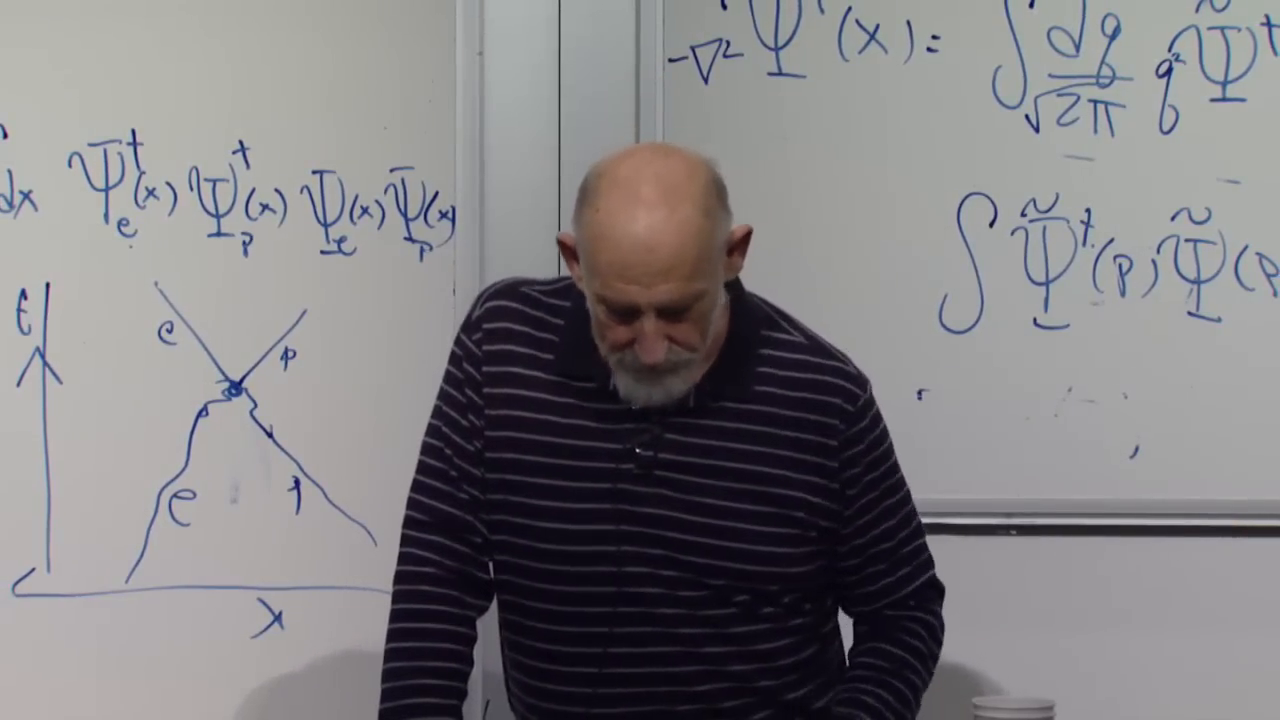
\includegraphics[width=0.94\linewidth]{lecture_09_frame_02.png}\caption{L’interaction de contact au tableau. Les quatre opérateurs de champ locaux figurent au-dessus du croquis d’espace-temps ; le point de rencontre est le seul endroit où agit l’interaction idéalisée.}\lectureframe{00:35:36}\end{figure}

\begin{figure}[htbp]\centering
\begin{tikzpicture}[x=1.2cm,y=1.0cm,>=Latex]
\draw[->] (-3.0,0) -- (3.0,0) node[right] {$x$};
\draw[->] (0,-0.2) -- (0,4.2) node[above] {$t$};
\coordinate (v) at (0,2.0);
\fill (v) circle (1.8pt);
\draw[thick,->] (-2.2,0.4) -- (v);
\draw[thick,->] (2.0,0.4) -- (v);
\draw[thick,->] (v) -- (-1.6,3.7);
\draw[thick,->] (v) -- (2.2,3.7);
\node[left] at (-1.65,0.7) {$e$};
\node[right] at (1.55,0.7) {$p$};
\node[left] at (-1.15,3.3) {$e$};
\node[right] at (1.65,3.3) {$p$};
\node[right] at (0.12,2.05) {$g$};
\end{tikzpicture}\caption{Reconstitution épurée du schéma de diffusion locale. Le sommet est une notation abrégée pour l’opérateur de l’équation ~\eqref{eq:l9-contact}, et non une loi classique de collision.}\end{figure}

Les électrons et les protons réels interagissent à distance par le potentiel coulombien. Le modèle de contact n’est qu’un premier pas, très limité : si l’expérience montrait que deux espèces ne diffusent que lorsqu’elles se recouvrent, l’équation ~\eqref{eq:l9-contact} serait le genre de terme que nous ajouterions au Hamiltonien.

\begin{classroomqa}
\lecturetimestamp{00:35:40}
\audiencequestion{Pourquoi cet opérateur de diffusion fait-il partie du Hamiltonien si l’énergie ne change pas ?}
\lecturerresponse{Le Hamiltonien est à la fois l’opérateur énergie et le générateur de l’évolution de l’état. Une énergie potentielle entre les deux particules produit de la diffusion au cours de l’évolution temporelle. La conservation de l’énergie totale ne signifie pas que l’état, ou les impulsions individuelles des particules, reste inchangé.}
\end{classroomqa}

Cela donne une règle pratique. Il faut d’abord apprendre par l’expérience quels processus locaux les particules peuvent subir. On encode ensuite ces processus dans l’opérateur qui fait évoluer l’état. Les produits de champs ne sont pas une algèbre décorative : leurs facteurs avec ou sans dagger précisent quelles espèces apparaissent et disparaissent.

\section{Désintégration, processus inverse et hermiticité}

Supposons qu’une chambre à bulles révèle la trace d’une espèce \(A\) qui se termine en un point d’où émergent les traces \(B\) et \(C\). Le processus local est
\begin{equation}
A\longrightarrow B+C.
\end{equation}
L’opérateur qui le réalise est
\begin{equation}
V=g\int dx\,
\psi_B^\dagger(x)\psi_C^\dagger(x)\psi_A(x).
\label{eq:l9-decay-half}
\end{equation}
Le champ d’annihilation enlève \(A\) ; les deux champs de création produisent \(B\) et \(C\) au même point. L’intégration avec un poids identique sur chaque \(x\) exprime l’invariance par translation spatiale et fournit immédiatement
\begin{equation}
p_A=p_B+p_C.
\end{equation}

Un Hamiltonien doit être hermitien. C’est ce qui rend \(e^{-itH}\) unitaire et préserve la probabilité totale. L’équation ~\eqref{eq:l9-decay-half} n’est pas hermitienne à elle seule ; nous devons donc ajouter son adjoint :
\begin{equation}
H_{\mathrm{int}}
=\int dx\left[
g\,\psi_B^\dagger\psi_C^\dagger\psi_A
+g^*\,\psi_A^\dagger\psi_C\psi_B
\right](x).
\label{eq:l9-hermitian-vertex}
\end{equation}
Pour un couplage réel \(g\), les deux coefficients sont identiques. La conjugaison hermitienne inverse l’ordre des opérateurs tout en échangeant les champs avec dagger et sans dagger. Dans ce modèle fictif bosonique, les champs d’espèces distinctes commutent, de sorte que cette inversion n’entraîne aucune difficulté supplémentaire.

Le second terme réalise le processus inverse,
\begin{equation}
B+C\longrightarrow A.
\end{equation}
Ainsi, un Hamiltonien fermé et unitaire qui permet la désintégration contient aussi l’amplitude de recombinaison. Cela ne garantit pas que les deux sens se produisent pour tout choix de moments extérieurs ; les lois de conservation de l’énergie et d’autres grandeurs peuvent rendre un sens inaccessible cinématiquement. Cela signifie que l’opérateur et son adjoint font tous deux partie de la dynamique.

\begin{classroomqa}
\lecturetimestamp{00:42:48}
\audiencequestion{Peut-il y avoir une exception à la règle selon laquelle le processus inverse est lui aussi permis ?}
\lecturerresponse{Pas au niveau d’un Hamiltonien hermitien pour un système fermé : l’interaction adjointe est nécessaire. Une réaction inverse particulière peut néanmoins être interdite par la cinématique ou par un autre nombre quantique conservé, mais l’élément de matrice conjugué est présent.}
\end{classroomqa}

Le nombre \(g\) est la constante de couplage. Si \(g\) est petit, les particules qui se rencontrent interagissent faiblement ; s’il est grand, l’amplitude de transition est plus élevée. Les couplages sont généralement des paramètres mesurés expérimentalement, bien que des symétries puissent relier plusieurs couplages apparemment différents.

La même grammaire permet de traiter des réactions plus élaborées. Dans la désintégration bêta,
\begin{equation}
n\longrightarrow p+e^-+\bar\nu_e,
\end{equation}
un terme local schématique contient quatre champs : l’un annihile le neutron et trois créent le proton, l’électron et l’antineutrino électronique, avec le processus hermitien conjugué. Cela suffit à montrer comment un petit nombre de monômes d’opérateurs commence à définir une théorie quantique des champs.

\section{Pourquoi le carré du Hamiltonien est important}

La formule à court terme \eqref{eq:l9-short-update} ne conservait que le premier ordre en \(\epsilon\). Le développement complet est
\begin{equation}
e^{-i\epsilon H}
=1-i\epsilon H-\frac{\epsilon^2}{2}H^2
+\frac{i\epsilon^3}{3!}H^3+\cdots.
\label{eq:l9-exponential}
\end{equation}
Au deuxième ordre, le Hamiltonien agit deux fois. C’est l’origine algébrique des premiers schémas représentant des processus composés.

Pour le sommet \(A\leftrightarrow B+C\), une action peut combiner \(B+C\) en \(A\), puis une seconde peut décomposer cet \(A\) de nouveau en \(B+C\) :
\begin{equation}
B+C\longrightarrow A\longrightarrow B+C.
\label{eq:l9-bc-scattering}
\end{equation}
La contribution nette est une amplitude de diffusion \(B+C\to B+C\). L’état intermédiaire \(A\) ne représente pas un événement observé supplémentaire ; il désigne l’état sur lequel on somme entre deux actions de l’interaction.

\begin{classroomqa}
\lecturetimestamp{00:49:54}
\audiencequestion{Dans le produit du deuxième ordre écrit au tableau, le champ \(C\) devrait-il porter un dagger ?}
\lecturerresponse{Oui, l’ordre des opérateurs doit correspondre à la séquence indiquée. Le premier sommet annihile \(B\) et \(C\) et crée \(A\) ; le second annihile \(A\) et recrée \(B\) et \(C\). L’écriture correcte des daggers correspondants rétablit cette interprétation.}
\end{classroomqa}

\begin{figure}[htbp]\centering
\includegraphics[width=0.94\linewidth]{lecture_09_frame_05.png}\caption{Les deux orientations du sommet élémentaire \(A\leftrightarrow B+C\) dessinées au tableau. Leur juxtaposition est la notation visuelle abrégée du processus du deuxième ordre de l’équation ~\eqref{eq:l9-bc-scattering}.}\lectureframe{00:48:56}\end{figure}

Ajoutons maintenant une particule spectatrice \(B\). Une action permet à \(A\) d’émettre \(C\) et de devenir \(B\) ; lors d’une action ultérieure, cet \(C\) se combine à l’\(B\) initial pour former \(A\). Les particules extérieures sont de nouveau \(A+B\), mais leurs impulsions peuvent changer. Nous décrivons cela comme une diffusion \(A\) et \(B\) par échange de \(C\).

\begin{figure}[htbp]\centering
\includegraphics[width=0.94\linewidth]{lecture_09_frame_06.png}\caption{Le mécanisme d’échange au tableau. Le diagramme de droite relie deux sommets élémentaires par une ligne interne de \(C\), tandis que les particules externes \(A\) et \(B\) diffusent.}\lectureframe{00:51:22}\end{figure}

\begin{figure}[htbp]\centering
\begin{tikzpicture}[x=1.1cm,y=1cm,>=Latex]
\draw[->] (-3.7,-0.2) -- (-3.7,4.2) node[above] {$t$};
\coordinate (v1) at (-0.9,1.25);
\coordinate (v2) at (0.9,2.95);
\fill (v1) circle (1.7pt);
\fill (v2) circle (1.7pt);
\draw[thick,->] (-2.6,0.2) -- (v1) node[midway,below left] {$A$};
\draw[thick,->] (2.6,0.2) -- (v2) node[midway,below right] {$B$};
\draw[thick,->] (v1) -- (-2.4,4.0) node[midway,left] {$B$};
\draw[thick,->] (v2) -- (2.5,4.0) node[midway,right] {$A$};
\draw[thick,->,dashed] (v1) -- (v2) node[midway,above left] {$C$};
\node[below] at (0,-0.05) {$A+B\rightarrow A+B$};
\end{tikzpicture}\caption{Reconstitution épurée de l’échange de \(C\). Chaque point apporte un facteur \(g\) ; ce terme du deuxième ordre est donc proportionnel à \(g^2\).}\end{figure}

Chaque point d’interaction locale est appelé un sommet. Chaque sommet apporte un facteur égal à son couplage ; une contribution à deux sommets comporte donc \(g^2\), une contribution à trois sommets \(g^3\), et ainsi de suite. Un seul terme du Hamiltonien relie ainsi toute une famille de réactions. Cette économie explique en partie la puissance de la théorie quantique des champs : un petit nombre d’interactions locales organise une quantité considérable de données de diffusion.

\begin{classroomqa}
\lecturetimestamp{00:53:14}
\audiencequestion{Comment appelle-t-on le processus \(A\to B+C\to A\) ?}
\lecturerresponse{C’est une contribution à l’auto-énergie. Un \(A\) mesuré n’est pas simplement l’état de base nu à une particule ; l’état en interaction possède aussi une amplitude pour des composantes \(B+C\) voisines. La diffusion sur cet état peut révéler cette structure habillée.}
\end{classroomqa}

L’électrodynamique quantique en fournit l’exemple familier. Un sommet local électron--photon peut annihiler un électron, recréer un électron et créer un photon. Au deuxième ordre, l’électron peut émettre un photon puis le réabsorber. On est tenté d’en faire le récit comme d’un petit film, mais son sens rigoureux est celui d’un terme du développement perturbatif. L’électron physique est un état habillé qui comporte des composantes contenant des photons.

L’estimation donnée en cours, selon laquelle cette composante est ``d’environ un pour cent'', donne une idée de l’échelle fixée par la constante de structure fine, \(\alpha_{\mathrm{em}}\simeq 1/137\). La probabilité précise d’une composante de Fock avec photon dépend de la résolution en énergie et de la définition de l’état en interaction ; ce n’est pas une propriété universelle de l’électron isolé, égale à un pour cent. L’énoncé robuste est que l’interaction modifie la structure mesurable de l’électron.

\section{Ce qu’un diagramme dit et ne dit pas}

Les diagrammes sont une notation abrégée, utile au calcul, pour les puissances du Hamiltonien d’interaction. Ils ne constituent pas des histoires classiques fiables dans lesquelles une particule accomplirait certainement un événement puis un autre. Chercher à déterminer si une alternative intermédiaire ``s’est réellement produite'' modifie l’expérience et détruit la somme cohérente, comme dans une expérience d’interférence quantique ordinaire.

\begin{classroomqa}
\lecturetimestamp{00:56:52}
\audiencequestion{L’énergie et la quantité de mouvement sont-elles toutes deux conservées au premier sommet ?}
\lecturerresponse{Dans la construction hamiltonienne à temps égal effectuée ici, l’intégrale spatiale produit immédiatement un delta de Dirac en impulsion. Aucune intégrale temporelle n’a encore produit de delta en énergie pour cette insertion isolée. L’amplitude de diffusion complète, invariante par translation temporelle, conserve l’énergie totale, tandis que les lignes intermédiaires n’ont pas nécessairement à satisfaire la relation de masse des particules observées. Dans le langage des diagrammes covariants, le quadri-moment est conservé à chaque sommet, mais les particules internes peuvent être hors couche de masse.}
\end{classroomqa}

L’énergie apparemment manquante dans une représentation naïve du sommet rappelle une fois de plus qu’il ne faut pas négliger l’énergie d’interaction. Le Hamiltonien total ne se réduit pas à la somme des énergies des particules libres. En cas de doute, revenons à l’équation ~\eqref{eq:l9-exponential} : le schéma représente un terme du développement de l’évolution unitaire dans le temps. La théorie complète des diagrammes de Feynman fournit un ordre temporel systématique, des propagateurs, des intégrales et des facteurs de symétrie, mais les bases physiques sont déjà là.

Une question plus développée pousse à interpréter le diagramme trop littéralement en comparant le photon émis au champ électrique entourant un électron en mouvement lent.

\begin{classroomqa}
\lecturetimestamp{00:58:26}
\audiencequestion{Le champ électrique de l’électron à distance est-il littéralement produit par des photons rayonnés ? Quel est le lien avec les interférences et l’effet Aharon--Bohm ?}
\lecturerresponse{Un champ statique ou un champ d’induction n’est pas un flux de photons réels rayonnés. L’électrodynamique quantique décrit à la fois le rayonnement et l’habillage électromagnétique de l’électron à l’aide du même champ, mais les états quantiques et les conditions cinématiques correspondants diffèrent. Pour un électron ultrarelativiste, certaines composantes du champ peuvent utilement être assimilées à un flux de photons presque réels ; pour un électron lent, une trajectoire littérale de photon est un modèle inadéquat. L’interférence à deux fentes et l’effet Aharon--Bohm sont eux aussi des phénomènes de champ non classiques, mais ils ne transforment pas ce diagramme d’auto-énergie en film mécanique.}
\end{classroomqa}

\begin{classroomqa}
\lecturetimestamp{01:01:28}
\audiencequestion{Pourquoi exactement un modèle classique du diagramme échoue-t-il ?}
\lecturerresponse{Parce que le calcul additionne de manière cohérente les amplitudes associées à toutes les alternatives intermédiaires permises. L’expérience rend ces schémas intuitifs, mais leur contenu littéral ne dépasse jamais le développement en opérateurs qui les définit. Ils constituent une façon compacte de calculer \(H^2,H^3,\ldots\), et non le compte rendu d’événements intermédiaires observés.}
\end{classroomqa}

\begin{classroomqa}
\lecturetimestamp{01:03:04}
\audiencequestion{L’interaction coulombienne ordinaire peut-elle émerger comme limite classique de l’échange de photons ?}
\lecturerresponse{Oui. Le calcul de l’amplitude appropriée médiée par un photon, suivi de la limite statique non relativiste, donne le potentiel coulombien. La dérivation est plus technique que le présent aperçu des opérateurs ; elle ne doit toujours pas être interprétée comme si un photon sautait littéralement d’une particule classique à une autre.}
\end{classroomqa}

\begin{classroomqa}
\lecturetimestamp{01:03:44}
\audiencequestion{Les constantes de couplage se calculent-elles à partir des produits de champs ?}
\lecturerresponse{Leurs valeurs numériques sont généralement des données expérimentales. Une symétrie peut les contraindre ou relier des couplages qui seraient autrement indépendants. Lorsqu’une telle relation prédit les intensités relatives de réactions distinctes et que l’expérience la confirme, cet accord est particulièrement instructif.}
\end{classroomqa}

\begin{classroomqa}
\lecturetimestamp{01:04:48}
\audiencequestion{Quel est le rôle d’une symétrie accidentelle par rapport à celui d’une symétrie de jauge ?}
\lecturerresponse{Une symétrie de jauge contraint directement la structure permise et les relations entre les couplages. Une symétrie accidentelle n’est pas imposée au niveau fondamental, mais émerge parce que toutes les interactions permises d’ordre inférieur la respectent par hasard. Elle peut néanmoins avoir des conséquences importantes, même si son origine et sa robustesse diffèrent de celles d’une symétrie de jauge.}
\end{classroomqa}

C’est tout pour l’instant sur la théorie non relativiste des champs. Nous avions promis d’aborder les fermions. Au lieu de les quantifier immédiatement en seconde quantification, nous allons d’abord comprendre l’équation relativiste à une particule que leurs opérateurs de champ doivent satisfaire.

\section{Pourquoi l’électron exige une description relativiste}

Commençons par une dimension spatiale. Ce n’est pas une restriction réaliste, mais elle élimine la complexité géométrique du spin en trois dimensions tout en préservant l’algèbre essentielle. L’électron est assez léger pour que les effets relativistes comptent même dans les atomes. Dans l’hydrogène, sa vitesse caractéristique est de l’ordre de
\begin{equation}
v\sim\alpha_{\mathrm{em}}c\approx 0.007c,
\end{equation}
soit environ un pour cent de la vitesse de la lumière. Pour les électrons internes d’un atome lourd, l’ordre de grandeur devient \(v\sim Z\alpha_{\mathrm{em}}c\), et les corrections relativistes peuvent donc être importantes. Que la curiosité historique ou la précision atomique ait fourni la motivation décisive, une équation de type Schr\"odinger relativiste est physiquement nécessaire.

La méthode habituelle de quantification part de la relation classique entre l’énergie et la quantité de mouvement. Dans le cas non relativiste,
\begin{equation}
E=\frac{p^2}{2m},
\end{equation}
et les substitutions
\begin{equation}
E\mapsto i\partial_t,
\qquad
p\mapsto-i\partial_x
\end{equation}
donnent
\begin{equation}
i\partial_t\varphi(x,t)
=-\frac{1}{2m}\partial_x^2\varphi(x,t).
\end{equation}

La relativité donne plutôt, avec \(c=1\),
\begin{equation}
E^2=p^2+m^2.
\label{eq:l9-rel-dispersion}
\end{equation}

\begin{figure}[htbp]\centering
\includegraphics[width=0.94\linewidth]{lecture_09_frame_07.png}\caption{Le passage au tableau de \(E=p^2/2m\) à la relation relativiste \(E^2=p^2+m^2\), avec \(c=1\).}\lectureframe{01:10:30}\end{figure}

Appliquer les substitutions à la relation au carré donne
\begin{equation}
-\partial_t^2\varphi
=\left(-\partial_x^2+m^2\right)\varphi,
\label{eq:l9-klein-gordon}
\end{equation}
ou, de manière équivalente,
\begin{equation}
\left(\partial_t^2-\partial_x^2+m^2\right)\varphi=0.
\end{equation}
C’est l’équation de Klein--Gordon. C’est une équation relativiste de champ parfaitement valable, en particulier pour les champs de spin nul. Mais l’équation recherchée pour l’électron doit être du premier ordre en temps,
\begin{equation}
i\partial_t\Psi=H\Psi,
\end{equation}
afin que \(H\) lui-même, et pas seulement \(H^2\), engendre l’évolution.

On pourrait formellement choisir
\begin{equation}
H=\sqrt{-\partial_x^2+m^2}.
\end{equation}
La racine carrée se définit sans difficulté dans l’espace des impulsions, où elle correspond à une multiplication par \(\sqrt{p^2+m^2}\), mais dans l’espace des positions, c’est un opérateur pseudo-différentiel non local. Il est mathématiquement bien défini, mais peu adapté à l’équation locale que nous cherchons. Repartons donc de zéro.

\section{Une onde sans masse se propageant vers la droite}

Considérons d’abord une particule sans masse se déplaçant vers la droite. Son énergie et son impulsion positives vérifient
\begin{equation}
E=p
\qquad (c=1).
\end{equation}
La quantification donne
\begin{equation}
i\partial_t\psi=-i\partial_x\psi,
\end{equation}
ou
\begin{equation}
(\partial_t+\partial_x)\psi=0.
\label{eq:l9-right-mover}
\end{equation}
Toute solution est de la forme
\begin{equation}
\psi(x,t)=f(x-t).
\end{equation}
Le profil reste rigide et se déplace vers la droite à la vitesse de la lumière.

Deux difficultés apparaissent immédiatement. Premièrement, si l’on laisse l’équation ~\eqref{eq:l9-right-mover} agir sur des modes de Fourier arbitraires, une impulsion négative a pour énergie \(E=p<0\), de sorte que le Hamiltonien n’est pas minoré. Imposer à la main \(p>0\) ne conserverait que les modes se propageant vers la droite et ne donnerait pas encore la théorie de l’électron que nous voulons. Deuxièmement, l’équation ne décrit qu’un seul sens de propagation : elle ne contient aucun électron ordinaire se déplaçant vers la gauche. Nous allons d’abord résoudre le problème des deux sens de propagation, en laissant les énergies négatives apparaître.

\section{Deux composantes et la matrice alpha}

Introduisons deux amplitudes,
\begin{equation}
\Psi(x,t)=
\begin{pmatrix}
\psi_1(x,t)\\[3pt]
\psi_2(x,t)
\end{pmatrix},
\end{equation}
où \(\psi_1\) correspond à la propagation vers la droite et \(\psi_2\) à la propagation vers la gauche dans la limite sans masse :
\begin{align}
(\partial_t+\partial_x)\psi_1&=0,
&
(\partial_t-\partial_x)\psi_2&=0.
\end{align}
La mécanique quantique autorise aussi des superpositions arbitraires des deux. Une particule peut donc avoir des amplitudes associées aux deux sens de propagation, au lieu de porter une étiquette classique fixée une fois pour toutes.

Ce degré de liberté supplémentaire à deux valeurs ressemble algébriquement au spin, mais, en une dimension, il ne s’agit pas d’un moment cinétique ordinaire. Définissons
\begin{equation}
\alpha=
\begin{pmatrix}
1&0\\
0&-1
\end{pmatrix}
=\sigma_3.
\label{eq:l9-alpha}
\end{equation}
Le vecteur propre de valeur propre \(+1\) correspond à la composante se propageant vers la droite, et celui de valeur propre \(-1\) à la composante se propageant vers la gauche. Dans la théorie sans masse, le hamiltonien est simplement
\begin{equation}
H=\alpha p,
\end{equation}
et les deux équations se réunissent en
\begin{equation}
i\partial_t\Psi=-i\alpha\partial_x\Psi.
\label{eq:l9-massless-dirac}
\end{equation}

\begin{classroomqa}
\lecturetimestamp{01:22:44}
\audiencequestion{Quel est le nom de la matrice diagonale qui distingue les deux composantes ?}
\lecturerresponse{En tant que matrice de Pauli, c’est \(\sigma_3\), et non \(\sigma_1\). Dans la notation de Dirac, pour la construction présente, nous l’appelons \(\alpha\). Son algèbre est l’algèbre de Pauli usuelle, même si, ici, elle distingue les directions et non le moment cinétique de spin.}
\end{classroomqa}

\begin{classroomqa}
\lecturetimestamp{01:23:32}
\audiencequestion{La construction prend-elle un sens plus géométrique en trois dimensions, où la direction est un vecteur ?}
\lecturerresponse{Oui. Le problème en trois dimensions exige une matrice pour chaque direction spatiale et conduit à une structure de spineur plus riche. Le modèle unidimensionnel reste néanmoins exact dans son propre cadre et isole l’algèbre essentielle entre gauche et droite, sans cette complexité supplémentaire.}
\end{classroomqa}

\begin{figure}[htbp]
\centering
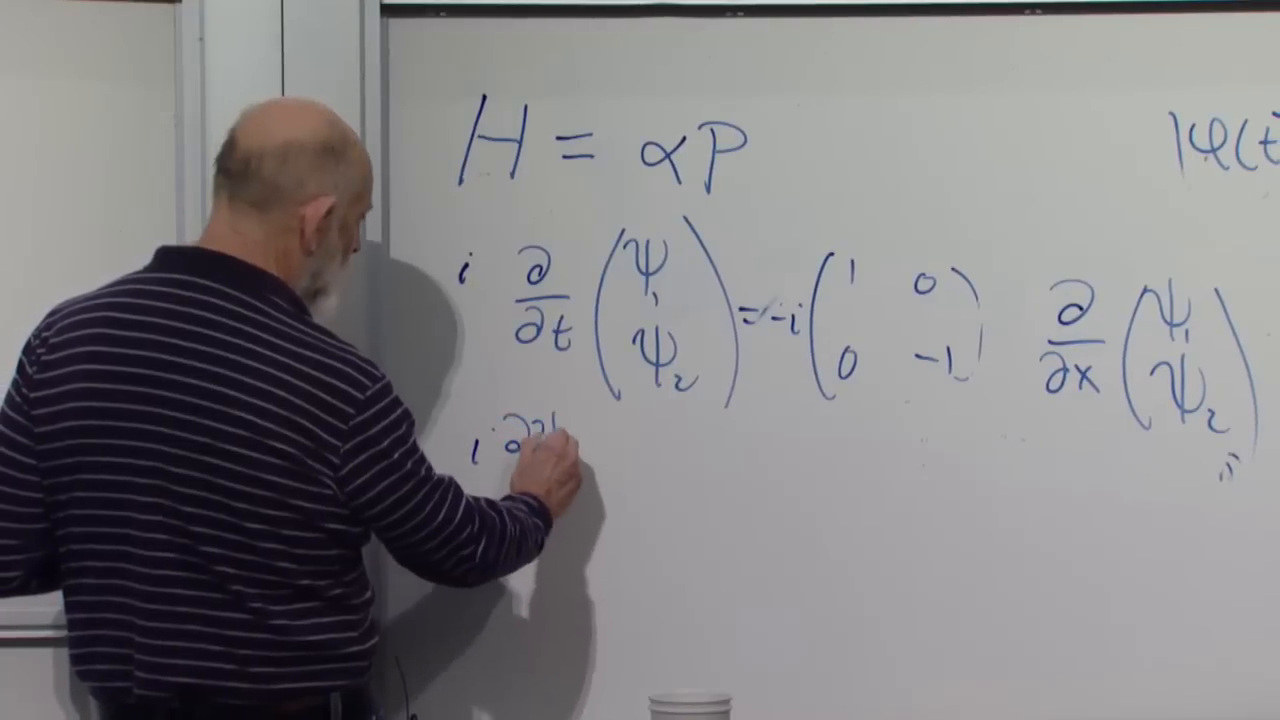
\includegraphics[width=0.94\linewidth]{lecture_09_frame_03.png}
\caption{L’équation sans masse à deux composantes inscrite au tableau : \(H=\alpha P\), où la matrice diagonale attribue des sens de propagation opposés à \(\psi_1\) et à \(\psi_2\).}
\lectureframe{01:26:00}
\end{figure}

Le problème de la propagation dans un seul sens est résolu. Le spectre d’énergie négative demeure, et nous avons découvert un troisième défaut : les deux composantes restent sans masse et se propagent à la vitesse de la lumière. L’étape suivante doit introduire une énergie au repos et coupler les directions.

\section{Ajout de la masse et découverte de l’algèbre de Dirac}

Ajoutons le terme simple le plus général proportionnel à la masse,
\begin{equation}
H=\alpha p+\beta m,
\label{eq:l9-dirac-hamiltonian}
\end{equation}
où \(\beta\) n’agit que sur l’indice des deux composantes. Il aurait pu s’agir de la matrice identité ou d’une autre matrice ; la relation de dispersion relativiste en décidera.

Puisque \(H^2\) doit être égal à \(p^2+m^2\), élevons au carré l’équation~\eqref{eq:l9-dirac-hamiltonian} :
\begin{align}
H^2
&=(\alpha p+\beta m)^2\\
&=\alpha^2p^2+\beta^2m^2
+(\alpha\beta+\beta\alpha)pm.
\label{eq:l9-square-dirac}
\end{align}
Les matrices commutent avec \(p\), car elles agissent sur l’espace interne des deux composantes, tandis que \(p\) agit sur la fonction d’onde spatiale. Pour retrouver l’équation~\eqref{eq:l9-rel-dispersion}, il faut que
\begin{equation}
\alpha^2=\mathbb{1},
\qquad
\beta^2=\mathbb{1},
\qquad
\{\alpha,\beta\}
=\alpha\beta+\beta\alpha=0.
\label{eq:l9-dirac-algebra}
\end{equation}
La première condition est déjà satisfaite par \(\alpha=\sigma_3\). Toute autre matrice de Pauli anticommmute avec elle et a pour carré la matrice identité. Choisissons
\begin{equation}
\beta=
\begin{pmatrix}
0&1\\
1&0
\end{pmatrix}
=\sigma_1.
\label{eq:l9-beta}
\end{equation}
Le choix de \(\sigma_1\) plutôt que de \(\sigma_2\) relève d’une convention de base ; les deux réalisent la même algèbre après un changement de base unitaire.

\begin{classroomqa}
\lecturetimestamp{01:33:00}
\audiencequestion{Dirac a-t-il simplement reconnu que les matrices de Pauli satisfont ces conditions algébriques ?}
\lecturerresponse{La dérivation historique a été menée directement en trois dimensions et a introduit des matrices satisfaisant les relations requises. Une fois les conditions écrites, l’algèbre de Pauli rend immédiate la solution unidimensionnelle : il suffit de choisir deux matrices de Pauli différentes.}
\end{classroomqa}

\begin{classroomqa}
\lecturetimestamp{01:34:24}
\audiencequestion{S’agit-il ici de \(\beta\), le paramètre relativiste de vitesse \(v/c\) ?}
\lecturerresponse{Non. C’est une matrice qui agit sur les composantes du spineur. Cette lettre réutilisée n’est que la notation de Dirac ; elle n’a rien à voir avec la quantité cinématique \(v/c\).}
\end{classroomqa}

En trois dimensions spatiales, les matrices \(2\times2\) ne suffisent pas pour obtenir l’ensemble complet des matrices anticommutantes requises. Cet élargissement sera abordé plus tard. En une dimension, les équations~\eqref{eq:l9-alpha} et \eqref{eq:l9-beta} suffisent.

\section{L’équation de Dirac unidimensionnelle couplée}

En substituant \(p=-i\partial_x\), on obtient l’équation de Dirac unidimensionnelle sous forme hamiltonienne :
\begin{equation}
i\partial_t\Psi
=\left(-i\alpha\partial_x+\beta m\right)\Psi.
\label{eq:l9-one-dimensional-dirac}
\end{equation}
Comme \(\alpha\) est diagonale, son terme dérivé laisse les deux composantes séparées. Comme \(\beta\) est hors diagonale, le terme de masse échange les deux composantes. Écrites composante par composante, les équations sont
\begin{align}
i\partial_t\psi_1
&=-i\partial_x\psi_1+m\psi_2,
\label{eq:l9-dirac-component-one}\\
i\partial_t\psi_2
&=+i\partial_x\psi_2+m\psi_1.
\label{eq:l9-dirac-component-two}
\end{align}

\begin{figure}[htbp]
\centering
\includegraphics[width=0.94\linewidth]{lecture_09_frame_08.png}
\caption{Les équations couplées des composantes inscrites au tableau. Les signes opposés devant les dérivées codent les propagations vers la droite et vers la gauche ; le terme de masse hors diagonale échange \(\psi_1\) et \(\psi_2\).}
\lectureframe{01:37:44}
\end{figure}

Dès que \(m\ne0\), les composantes cessent d’évoluer indépendamment. En élevant au carré l’équation du premier ordre, on retrouve l’opérateur de Klein--Gordon sur chaque composante,
\begin{equation}
\left(\partial_t^2-\partial_x^2+m^2\right)\psi_a=0,
\qquad a=1,2,
\end{equation}
et les ondes planes satisfont \(E^2=p^2+m^2\). Leur vitesse de groupe est
\begin{equation}
v_g=\frac{dE}{dp}=\frac{p}{E},
\end{equation}
et sa valeur absolue est inférieure à un pour toute masse non nulle.

Le lien entre la masse et le mélange des composantes droite et gauche n’est pas fortuit. Un mode se propageant vers la droite et sans masse reste dirigé vers la droite sous toute transformation de Lorentz propre ; aucun observateur subluminal ne peut dépasser la lumière et en inverser le sens. Une particule massive peut être amenée au repos, puis observée dans un référentiel plus rapide se déplaçant dans le même sens, où sa vitesse apparaît inversée. Une théorie relativiste massive ne peut donc pas maintenir les secteurs droit et gauche isolés en permanence. Le terme de masse hors diagonale fournit précisément le couplage nécessaire.

\begin{classroomqa}
\lecturetimestamp{01:40:01}
\audiencequestion{L’échange entre les deux composantes est-il une oscillation chirale ?}
\lecturerresponse{Dans cette base unidimensionnelle, \(\alpha\) distingue les deux directions chirales sans masse. Le terme de masse est hors diagonale et les mélange ; la chiralité n’est donc plus conservée. En ce sens, le terme de masse est à l’origine de l’oscillation chirale.}
\end{classroomqa}

\begin{classroomqa}
\lecturetimestamp{01:40:46}
\audiencequestion{Pourquoi l’équation d’un fermion devrait-elle être la racine carrée de celle d’un boson ?}
\lecturerresponse{Il ne faut pas comprendre les choses ainsi. La relation de dispersion \(E^2=p^2+m^2\) s’applique à toute particule relativiste libre, quelles que soient ses statistiques. L’opérateur de Dirac fournit une factorisation matricielle de l’opérateur de Klein--Gordon, mais cette relation algébrique ne dérive pas les fermions des bosons.}
\end{classroomqa}

\begin{classroomqa}
\lecturetimestamp{01:41:31}
\audiencequestion{Peut-on réduire l’équation à une factorisation scalaire simple en facteurs distincts correspondant aux propagations vers la gauche et vers la droite ?}
\lecturerresponse{Ce n’est que dans la limite sans masse que les deux équations chirales se découplent en facteurs scalaires indépendants. Pour \(m\ne0\), la factorisation utile est matricielle : ce sont les matrices anticommutantes \(\alpha\) et \(\beta\) qui éliminent le terme croisé indésirable.}
\end{classroomqa}

\begin{classroomqa}
\lecturetimestamp{01:42:04}
\audiencequestion{Ces deux équations couplées constituent-elles déjà l’équation de Dirac ?}
\lecturerresponse{Oui. Ensemble, elles forment l’équation de Dirac en une dimension spatiale, écrite de façon équivalente sous la forme compacte de l’équation~\eqref{eq:l9-one-dimensional-dirac}. On peut obtenir une notation covariante plus symétrique en multipliant par \(\beta\), mais cette forme sera présentée plus tard.}
\end{classroomqa}

Deux tâches restent délibérément inachevées. La construction n’a pas éliminé les énergies négatives ; elle a fourni des solutions d’énergie négative dans les deux secteurs directionnels, de sorte que le problème apparaît maintenant plus clairement, et non moins. Et la théorie demeure limitée à une dimension spatiale. L’interprétation des solutions d’énergie négative et l’élargissement de l’algèbre des matrices aux dimensions \(3+1\) sont les prochaines étapes.

\chapter{Fermions, matrices de Dirac et mer de Dirac}

La mer de Dirac est notre destination, mais le chemin compte. Avant d’aborder l’énergie négative dans la théorie relativiste de l’électron, nous avons besoin de deux outils. Nous commencerons par l’algèbre des opérateurs qui distingue les fermions des bosons. Nous reverrons ensuite l’équation de Dirac à une dimension, où l’on peut observer chaque élargissement de la fonction d’onde sans la géométrie des trois dimensions spatiales. Une fois ces éléments en place, l’équation tridimensionnelle imposera sa propre structure matricielle, et la discussion initiale des états fermioniques occupés et inoccupés reviendra comme clé de compréhension des positrons.

Nous posons \(c=\hbar=1\). La lettre majuscule \(P\) désigne un opérateur impulsion, la lettre minuscule \(p\) une valeur propre de l’impulsion, et les symboles en gras leurs versions tridimensionnelles.

\section{L’échange devient une algèbre d’opérateurs}

Considérons deux particules identiques, l’une en \(x\), l’autre en \(y\). Les étiquettes \(x\) et \(y\) désignent des positions complètes ; ce ne sont pas deux coordonnées cartésiennes d’une seule particule. L’action de deux opérateurs de création sur le vide donne
\begin{equation}
\lvert x,y\rangle
=
\psi^\dagger(x)\psi^\dagger(y)\lvert0\rangle.
\label{eq:l10-two-particle-state}
\end{equation}

Pour des bosons, l’échange des deux places laisse l’état inchangé :
\begin{equation}
\lvert x,y\rangle=\lvert y,x\rangle.
\end{equation}
L’énoncé en termes d’opérateurs qui garantit cette symétrie est
\begin{equation}
\psi^\dagger(x)\psi^\dagger(y)
=
\psi^\dagger(y)\psi^\dagger(x).
\label{eq:l10-boson-exchange}
\end{equation}
Deux opérateurs de création bosoniques commutent ; on peut donc inverser leur ordre sans changer l’état qu’ils créent.

Pour des fermions, l’échange change le signe :
\begin{equation}
\lvert x,y\rangle=-\lvert y,x\rangle.
\label{eq:l10-fermion-state-exchange}
\end{equation}
Le signe global d’un vecteur d’état isolé n’est pas observable, mais les signes relatifs entre plusieurs possibilités le sont ; il faut donc conserver ce signe moins de manière cohérente. L’équation~\eqref{eq:l10-fermion-state-exchange} impose
\begin{equation}
\psi^\dagger(x)\psi^\dagger(y)
=
-\,\psi^\dagger(y)\psi^\dagger(x).
\label{eq:l10-fermion-operator-exchange}
\end{equation}

\begin{figure}[htbp]
\centering
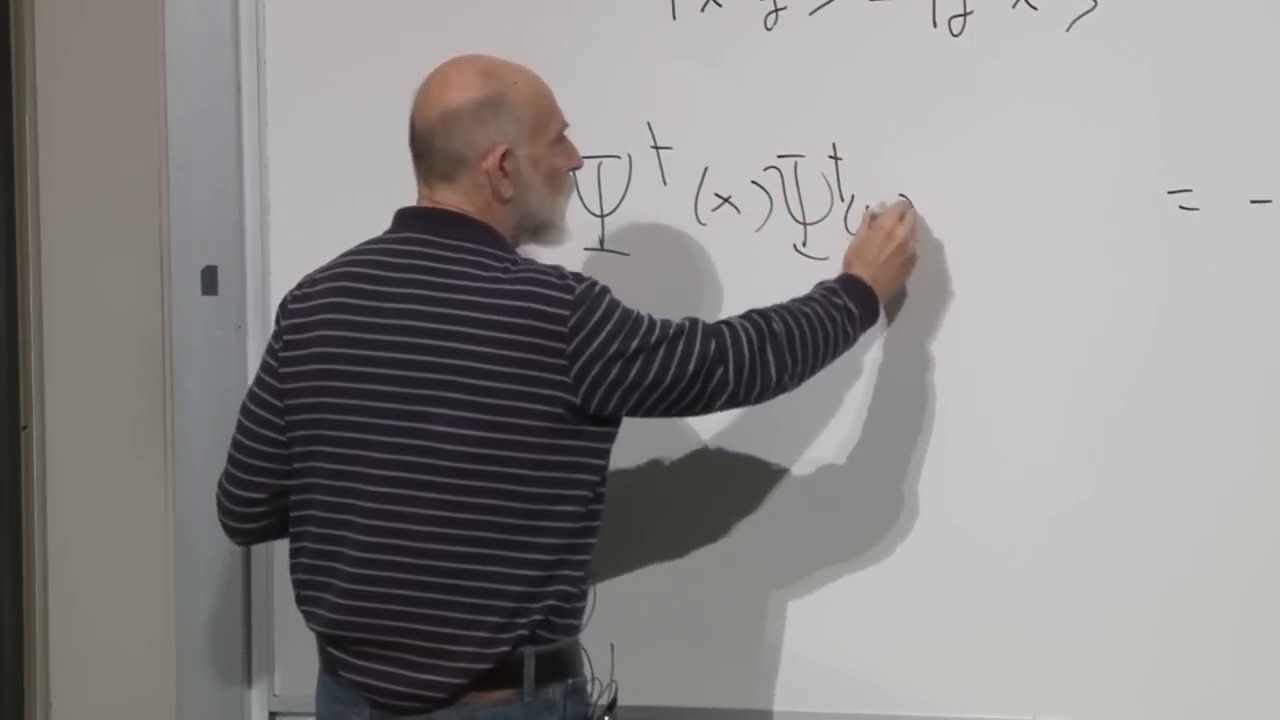
\includegraphics[width=0.94\linewidth]{lecture_10_figure_02.png}
\caption{La relation d’échange fermionique inscrite au tableau. L’inversion de l’ordre des opérateurs de création change le signe de l’état à deux particules.}
\lectureframe{00:05:50}
\end{figure}

Pour deux opérateurs quelconques \(A\) et \(B\), définissons l’anticommutateur par
\begin{equation}
\{A,B\}:=AB+BA.
\end{equation}
La règle d’échange s’écrit donc
\begin{equation}
\{\psi^\dagger(x),\psi^\dagger(y)\}=0.
\label{eq:l10-creation-anticommutator}
\end{equation}
L’algèbre correspondante des champs fermioniques remplace les commutateurs bosoniques par des anticommutateurs. Il faut distinguer les deux emplois du mot : les opérateurs de champ anticommutent en raison de la statistique de Fermi, tandis que les matrices anticommuteront plus tard afin d’annuler les termes croisés dans une relation de dispersion relativiste.

Posons maintenant \(y=x\) dans l’équation~\eqref{eq:l10-creation-anticommutator}. Les deux produits deviennent identiques :
\begin{align}
0
&=\{\psi^\dagger(x),\psi^\dagger(x)\}\\
&=2\,\psi^\dagger(x)\psi^\dagger(x).
\end{align}
Par conséquent,
\begin{equation}
\bigl(\psi^\dagger(x)\bigr)^2=0.
\label{eq:l10-exclusion}
\end{equation}
La tentative de créer deux fermions identiques dans le même état à une particule donne le vecteur nul. C’est le principe d’exclusion sous forme opératorielle.

\begin{figure}[htbp]
\centering
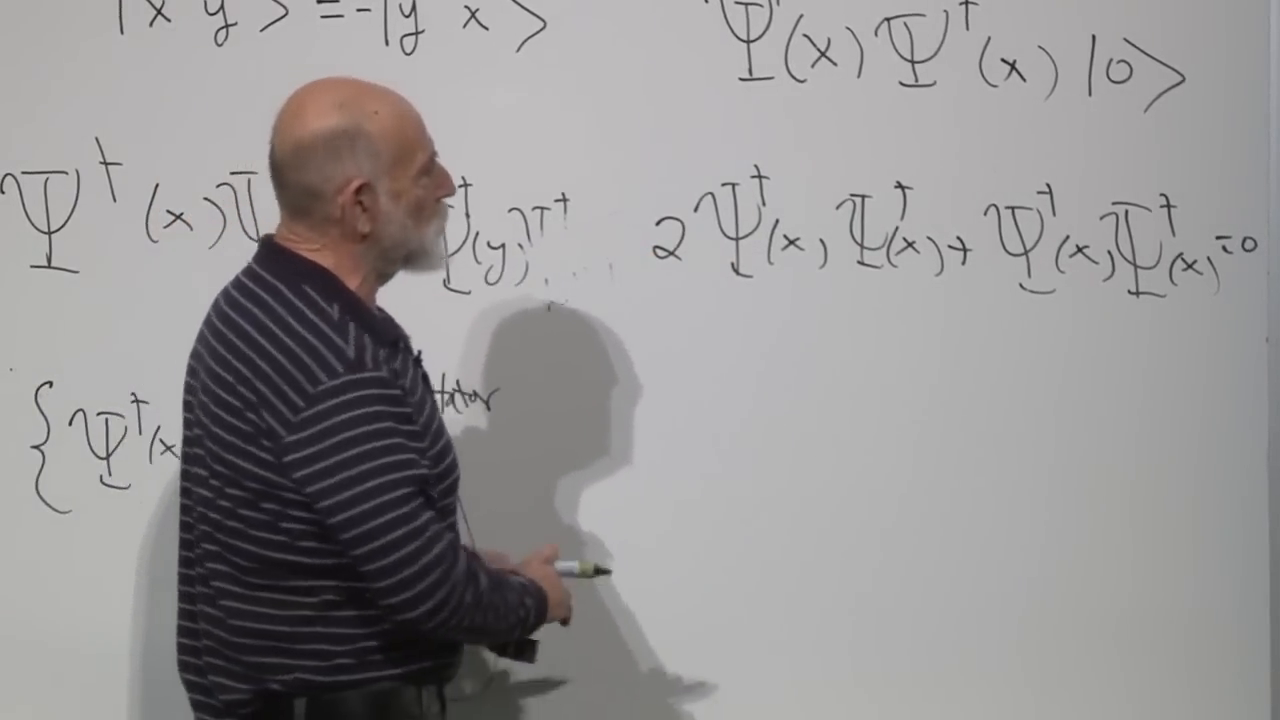
\includegraphics[width=0.94\linewidth]{lecture_10_figure_03.png}
\caption{Le cas particulier d’états identiques au tableau. Le produit répété d’opérateurs de création apparaît deux fois et doit donc s’annuler.}
\lectureframe{00:08:04}
\end{figure}

\begin{figure}[htbp]
\centering
\begin{adjustbox}{max width=\linewidth}
\begin{tikzpicture}[node distance=1.25cm,>=Latex]
\node[draw,rounded corners,align=center,inner sep=7pt] (a)
  {$\{\psi^\dagger(x),\psi^\dagger(x)\}=0$};
\node[draw,rounded corners,align=center,inner sep=7pt,right=of a] (b)
  {$2(\psi^\dagger(x))^2=0$};
\node[draw,rounded corners,align=center,inner sep=7pt,right=of b] (c)
  {$(\psi^\dagger(x))^2=0$};
\draw[->,thick] (a) -- (b);
\draw[->,thick] (b) -- (c);
\end{tikzpicture}
\end{adjustbox}
\caption{La démonstration de l’exclusion reconstituée sans les étapes intermédiaires partiellement effacées du tableau.}
\end{figure}

\section{Pourquoi l’occupation et l’absence d’occupation sont symétriques pour un fermion}

Il existe une autre différence entre les opérateurs bosoniques et fermioniques, plus subtile que l’exclusion et essentielle pour la suite. Pour un mode bosonique unique,
\begin{equation}
[a,a^\dagger]=1,
\qquad
n=0,1,2,\ldots.
\end{equation}
L’inversion de l’ordre de \(a\) et \(a^\dagger\) change le signe du commutateur. Même si l’on appelait simplement les opérateurs \(A\) et \(B\), l’algèbre nous indiquerait lequel augmente le nombre d’occupation et lequel le diminue.

L’échelle d’occupation bosonique a aussi une orientation. L’opérateur d’annihilation finit par atteindre \(\lvert0\rangle\) et donne zéro, tandis que l’opérateur de création peut continuer indéfiniment :
\begin{align}
a\lvert0\rangle&=0,\\
a^\dagger\lvert n\rangle&\propto\lvert n+1\rangle,
\qquad n=0,1,2,\ldots.
\end{align}
Retourner cette échelle ne reproduit pas le même spectre. Il y a un minimum, mais pas de maximum.

Pour un mode fermionique unique,
\begin{equation}
\{a,a^\dagger\}=1,
\qquad
a^2=(a^\dagger)^2=0,
\qquad
n=0,1.
\label{eq:l10-fermion-mode}
\end{equation}
L’opérateur de création fait passer de l’état inoccupé à l’état occupé, puis s’arrête :
\begin{equation}
a^\dagger\lvert0\rangle=\lvert1\rangle,
\qquad
a^\dagger\lvert1\rangle=0.
\end{equation}
L’opérateur d’annihilation effectue l’opération inverse :
\begin{equation}
a\lvert1\rangle=\lvert0\rangle,
\qquad
a\lvert0\rangle=0.
\end{equation}
Il n’y a que deux états ; le diagramme est donc symétrique si l’on échange l’état occupé et l’état inoccupé, ainsi que \(a\) et \(a^\dagger\). Les opérateurs gardent des significations physiques différentes, mais leur algèbre ne distingue plus l’un comme opérateur de création et l’autre comme opérateur d’annihilation. Cette symétrie formelle est à l’origine de la réinterprétation en termes de particule-trou.

\begin{classroomqa}
\lecturetimestamp{00:13:54}
\audiencequestion{Si \((a^\dagger)^2=0\), est-ce contradictoire, ou cela implique-t-il que \(a^\dagger=0\) ?}
\lecturerresponse{Ni l’un ni l’autre. Un opérateur non nul peut avoir un carré nul. Ici, \(a^\dagger\) fait passer \(\lvert0\rangle\) à \(\lvert1\rangle\), mais aucun état autorisé ne se trouve au-dessus de \(\lvert1\rangle\) ; une seconde application donne donc zéro. Le même raisonnement donne \(a^2=0\).}
\end{classroomqa}

Gardons cette symétrie entre état occupé et état inoccupé à l’esprit. Lorsqu’un électron d’énergie négative sera retiré, l’opérateur d’annihilation sera renommé opérateur de création de positron. Ce changement n’est pas une modification arbitraire de la notation : il repose précisément sur l’algèbre fermionique à deux états établie ici.

\section{La construction de Dirac à une dimension}

Revenons maintenant à une particule dans une seule dimension spatiale. L’équation d’onde relativiste du premier ordre la plus simple est
\begin{equation}
i\partial_t\psi=-\,i\partial_x\psi.
\label{eq:l10-right-mover}
\end{equation}
Avec \(P=-i\partial_x\), on obtient
\begin{equation}
H=P.
\end{equation}
Un état propre de l’impulsion vérifie \(E=p\), et sa vitesse de groupe est
\begin{equation}
v_g=\frac{dE}{dp}=1.
\end{equation}
Que l’impulsion, et donc l’énergie, soit positive ou négative, l’onde se propage toujours vers la droite sans se déformer. Le signe de \(p\) modifie la structure de phase, pas le sens de propagation.

Une particule massive doit pouvoir se déplacer dans les deux sens. Introduisons une seconde composante qui vérifie
\begin{equation}
H\psi_1=P\psi_1,
\qquad
H\psi_2=-P\psi_2.
\label{eq:l10-two-directions}
\end{equation}
La première composante se propage vers la droite ; la seconde, vers la gauche. Regroupons-les dans une colonne,
\begin{equation}
\Psi=
\begin{pmatrix}
\psi_1\\
\psi_2
\end{pmatrix},
\end{equation}
et définissons
\begin{equation}
\alpha=
\begin{pmatrix}
1&0\\
0&-1
\end{pmatrix}.
\end{equation}
Les deux équations deviennent
\begin{equation}
H\Psi=\alpha P\Psi.
\label{eq:l10-massless-one-d}
\end{equation}
Inclure les deux sens de propagation a pour contrepartie l’introduction d’un nouveau degré de liberté interne à deux valeurs.

Le seul sens de propagation ne produit pas la masse. Introduisons une seconde matrice,
\begin{equation}
\beta=
\begin{pmatrix}
0&1\\
1&0
\end{pmatrix},
\end{equation}
et essayons
\begin{equation}
H=\alpha P+\beta m.
\label{eq:l10-massive-one-d}
\end{equation}
Les matrices vérifient
\begin{equation}
\alpha^2=\beta^2=\mathbb{1},
\qquad
\{\alpha,\beta\}=0.
\label{eq:l10-one-d-algebra}
\end{equation}
En élevant le Hamiltonien au carré, on obtient
\begin{align}
H^2
&=(\alpha P+\beta m)^2\\
&=\alpha^2P^2+\beta^2m^2
  +(\alpha\beta+\beta\alpha)Pm\\
&=P^2+m^2.
\label{eq:l10-one-d-dispersion}
\end{align}
L’anticommutateur de l’équation~\eqref{eq:l10-one-d-algebra} élimine le terme indésirable, linéaire à la fois en \(P\) et en \(m\).

La matrice hors diagonale \(\beta\) couple les deux composantes associées aux sens de propagation. On peut se représenter le terme de masse comme un mélange continu des amplitudes se propageant vers la droite et vers la gauche. Il ne faut pas prendre cette image au pied de la lettre, comme si la particule rebondissait le long d’une trajectoire microscopique ; elle permet toutefois de comprendre pourquoi un paquet d’ondes massif peut avoir une vitesse moyenne inférieure à celle de la lumière et posséder un référentiel de repos, contrairement à une composante chirale sans masse isolée.

\begin{classroomqa}
\lecturetimestamp{00:23:37}
\audiencequestion{L’introduction de deux composantes associées aux sens de propagation a-t-elle une interprétation physique plus profonde ?}
\lecturerresponse{Oui, mais elle apparaît plus clairement en trois dimensions. À ce stade, il s’agit simplement des deux composantes nécessaires pour décrire les sens de propagation opposés et permettre un couplage de masse hors diagonale. Leur interprétation ultérieure sera la chiralité.}
\end{classroomqa}

\section{Les trois dimensions imposent les matrices de Pauli}

En trois dimensions spatiales, l’impulsion est un vecteur. Un Hamiltonien linéaire en l’impulsion et scalaire sous les rotations suggère donc un autre vecteur, dont les composantes sont cette fois des matrices :
\begin{equation}
H=\boldsymbol{\alpha}\cdot\mathbf P
=\alpha_xP_x+\alpha_yP_y+\alpha_zP_z.
\label{eq:l10-three-d-ansatz}
\end{equation}

\begin{figure}[htbp]
\centering
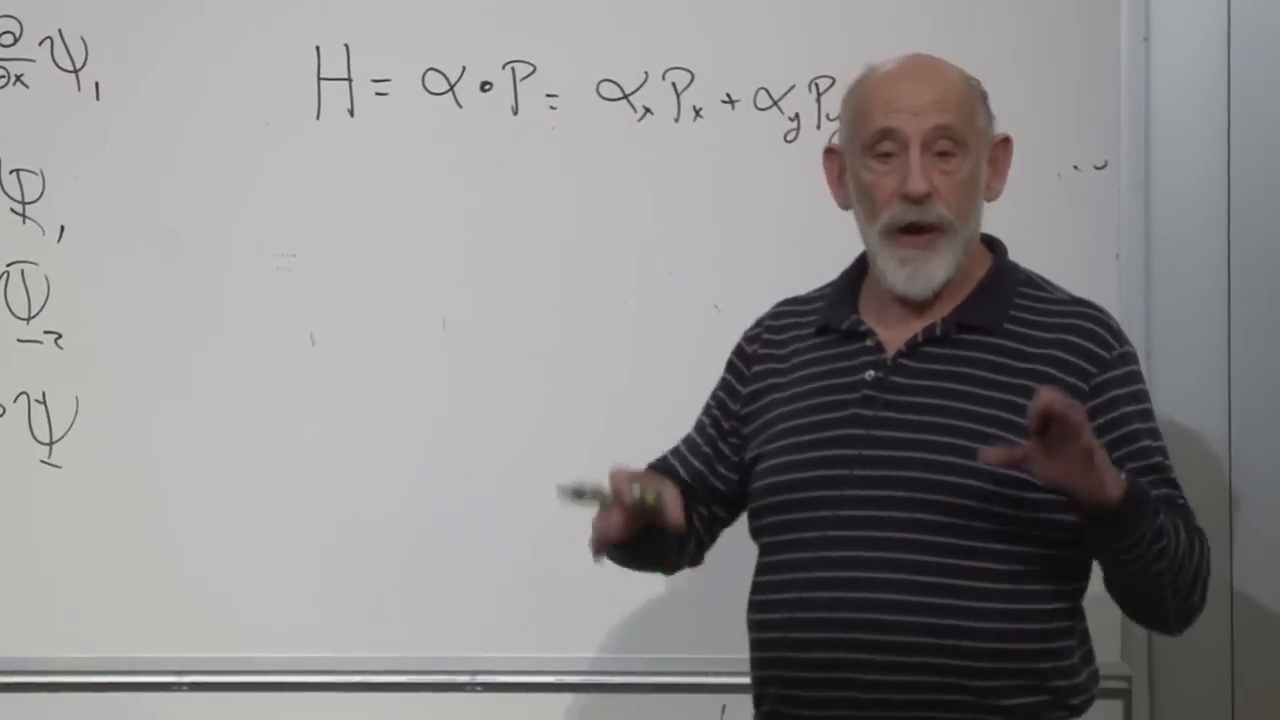
\includegraphics[width=0.94\linewidth]{lecture_10_figure_04.png}
\caption{L’ansatz sans masse tridimensionnel \(H=\boldsymbol{\alpha}\cdot\mathbf P\), au moment où une matrice devient un vecteur de trois matrices.}
\lectureframe{00:26:00}
\end{figure}

Repartons du cas sans masse. Nous imposons
\begin{equation}
H^2=\mathbf P^2=P_x^2+P_y^2+P_z^2.
\end{equation}
En développant le carré de l’équation~\eqref{eq:l10-three-d-ansatz},
\begin{align}
H^2
&=\alpha_x^2P_x^2+\alpha_y^2P_y^2\\
&\quad+\alpha_z^2P_z^2\\
&\quad+\{\alpha_x,\alpha_y\}P_xP_y\\
&\quad+\{\alpha_x,\alpha_z\}P_xP_z\\
&\quad+\{\alpha_y,\alpha_z\}P_yP_z.
\end{align}
Les termes diagonaux sont corrects si
\begin{equation}
\alpha_x^2=\alpha_y^2=\alpha_z^2=\mathbb{1},
\end{equation}
et tous les termes croisés s’annulent si
\begin{equation}
\{\alpha_i,\alpha_j\}=0,
\qquad i\ne j.
\label{eq:l10-alpha-anticommutation}
\end{equation}

Trois matrices \(2\times2\) bien connues satisfont précisément ces conditions :
\begin{equation}
\sigma_x=
\begin{pmatrix}
0&1\\
1&0
\end{pmatrix},
\quad
\sigma_y=
\begin{pmatrix}
0&-i\\
i&0
\end{pmatrix},
\quad
\sigma_z=
\begin{pmatrix}
1&0\\
0&-1
\end{pmatrix}.
\label{eq:l10-pauli-matrices}
\end{equation}
Une solution est donc
\begin{equation}
\alpha_i=\sigma_i,
\qquad
H=\boldsymbol{\sigma}\cdot\mathbf P.
\label{eq:l10-weyl-hamiltonian}
\end{equation}

\begin{figure}[htbp]
\centering
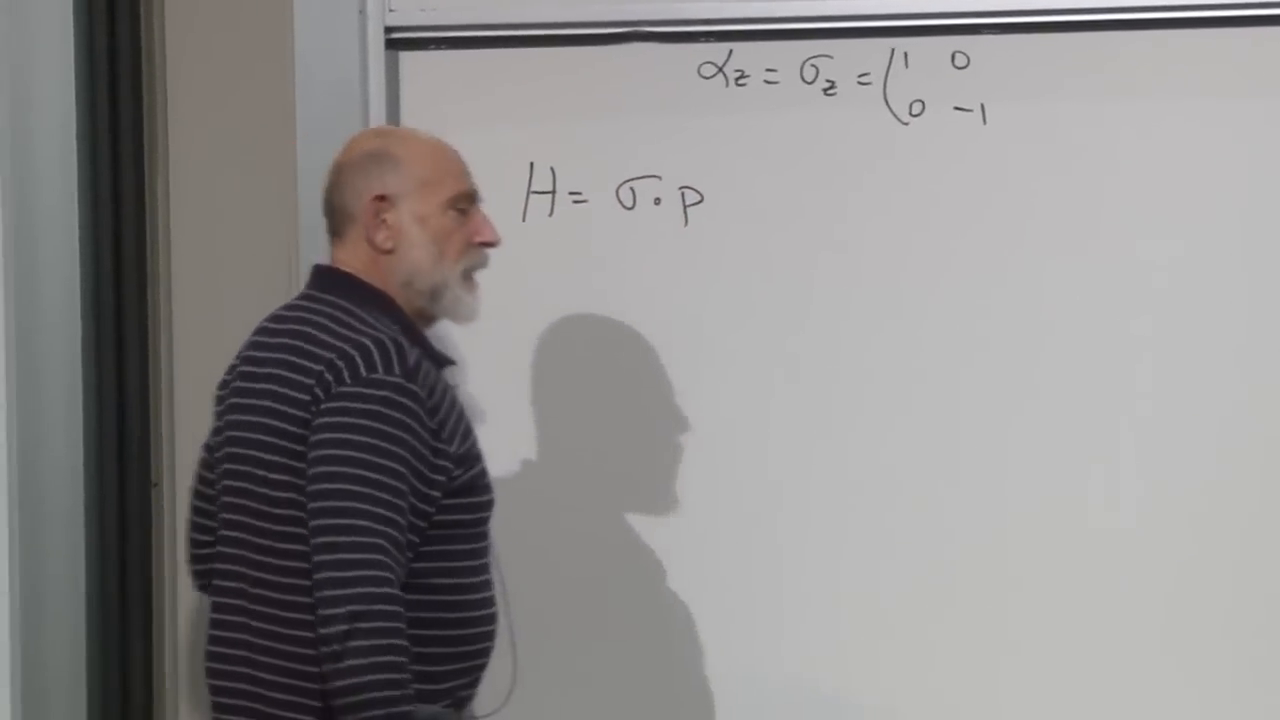
\includegraphics[width=0.94\linewidth]{lecture_10_figure_05.png}
\caption{Le Hamiltonien sans masse sous forme compacte \(H=\boldsymbol{\sigma}\cdot\mathbf P\), avec \(\alpha_z=\sigma_z\) encore visible au-dessus.}
\lectureframe{00:28:16}
\end{figure}

Pour un état propre de l’impulsion,
\begin{equation}
\boldsymbol{\sigma}\cdot\mathbf p
=
|\mathbf p|\,\boldsymbol{\sigma}\cdot\widehat{\mathbf p}.
\end{equation}
L’opérateur \(\boldsymbol{\sigma}\cdot\widehat{\mathbf p}\) a pour valeurs propres \(+1\) et \(-1\), donc
\begin{equation}
E=\pm|\mathbf p|.
\end{equation}
Dans cette théorie à deux composantes, pour une énergie positive, le degré de liberté de Pauli est aligné sur l’impulsion ; pour une énergie négative, il lui est anti-aligné. Cet alignement est fixé : pour un signe d’énergie donné, la direction du spin ne peut pas être réglée indépendamment.

\begin{classroomqa}
\lecturetimestamp{00:30:10}
\audiencequestion{Le spin découle-t-il de l’équation de Dirac, ou a-t-il été introduit parce que l’on sait déjà que l’électron possède un moment magnétique ?}
\lecturerresponse{Ici, « découler » signifie « apparaître comme conséquence », et non « disparaître ». Le point de départ était l’exigence d’un Hamiltonien linéaire en l’impulsion dont le carré soit \(\mathbf P^2\). Des nombres ordinaires ne peuvent satisfaire l’algèbre requise, contrairement aux matrices de Pauli. Leur structure à deux composantes apparaît donc dès la linéarisation. Cela ne prouve pas que toute particule doit avoir un spin ; cela signifie que les particules décrites par cette équation de type Dirac portent le degré de liberté spinoriel correspondant.}
\end{classroomqa}

C’est l’une des leçons centrales de cette construction. Les matrices ne sont pas des étiquettes décoratives ajoutées après avoir trouvé l’équation relativiste. C’est la tentative de prendre une racine carrée locale de la relation de dispersion relativiste qui les fait apparaître.

\section{Pourquoi la masse exige quatre composantes}

Essayons de reprendre la construction de la masse à une dimension sans élargir la théorie \(2\times2\) :
\begin{equation}
H=\boldsymbol{\sigma}\cdot\mathbf P+\beta m.
\label{eq:l10-failed-mass}
\end{equation}
Supposons \(\beta^2=\mathbb{1}\). Le carré contient les termes voulus \(\mathbf P^2+m^2\), mais aussi
\begin{equation}
m\sum_i\{\sigma_i,\beta\}P_i.
\end{equation}
Pour éliminer ce terme, une matrice \(\beta\) devrait vérifier
\begin{equation}
\{\sigma_x,\beta\}
=
\{\sigma_y,\beta\}
=
\{\sigma_z,\beta\}
=0.
\label{eq:l10-impossible-beta}
\end{equation}
Aucune matrice \(2\times2\) ne le peut. L’identité commute avec les trois matrices de Pauli, et toute matrice \(2\times2\) sans trace est une combinaison linéaire de matrices de Pauli. Aucune combinaison de ce type n’anticommute avec la composante qui lui est parallèle. L’algèbre \(2\times2\) ne contient pas de quatrième matrice indépendante répondant à la condition requise.

La solution consiste à élargir le spineur. Quatre matrices qui anticommuttent deux à deux et dont les carrés sont l’identité apparaissent pour la première fois dans une représentation complexe \(4\times4\). Cette taille de matrice n’est pas choisie parce que l’espace-temps a quatre dimensions ; c’est le plus petit espace matriciel capable de réaliser l’algèbre requise.

Il existe de nombreuses représentations équivalentes. Un changement unitaire de base du spineur modifie les éléments de toutes les matrices sans changer aucune prédiction physique. Ce qui importe, c’est l’ensemble abstrait des relations
\begin{equation}
\{\alpha_i,\alpha_j\}=2\delta_{ij}\mathbb{1},
\qquad
\{\alpha_i,\beta\}=0,
\qquad
\beta^2=\mathbb{1}.
\label{eq:l10-dirac-algebra}
\end{equation}

\begin{classroomqa}
\lecturetimestamp{00:37:38}
\audiencequestion{Peut-on considérer \(\beta\) comme une composante temporelle \(\alpha_t\) ?}
\lecturerresponse{Pas directement. Les trois \(\alpha_i\) ne se combinent pas avec \(\beta\) pour former les quatre composantes d’un même vecteur de Lorentz. En notation covariante, on définit plutôt \(\beta=\gamma^0\) et \(\alpha_i=\gamma^0\gamma^i\) ; les quatre matrices \(\gamma^\mu\) satisfont l’algèbre de Clifford de l’espace-temps.}
\end{classroomqa}

Une représentation par blocs commode est
\begin{equation}
\alpha_i=
\begin{pmatrix}
\sigma_i&0\\
0&-\sigma_i
\end{pmatrix},
\qquad
\beta=
\begin{pmatrix}
0&I_2\\
I_2&0
\end{pmatrix}.
\label{eq:l10-block-representation}
\end{equation}
Les matrices de Pauli dans les blocs diagonaux garantissent que les différentes matrices \(\alpha_i\) anticommuttent. Les blocs d’identité hors diagonale de \(\beta\) garantissent que \(\beta\) anticommute avec chacune des matrices \(\alpha_i\).

\begin{figure}[htbp]
\centering
\includegraphics[width=0.94\linewidth]{lecture_10_figure_06.png}
\caption{La représentation par blocs \(4\times4\) inscrite au tableau. Les équations du haut indiquent les anticommutateurs requis ; les matrices complètes sont composées dans l’équation~\eqref{eq:l10-block-representation}.}
\lectureframe{00:41:10}
\end{figure}

Le Hamiltonien massif s’écrit maintenant
\begin{equation}
H=\boldsymbol{\alpha}\cdot\mathbf P+\beta m
=
\begin{pmatrix}
\boldsymbol{\sigma}\cdot\mathbf P&mI_2\\
mI_2&-\boldsymbol{\sigma}\cdot\mathbf P
\end{pmatrix}.
\label{eq:l10-massive-dirac}
\end{equation}
En utilisant l’équation~\eqref{eq:l10-dirac-algebra},
\begin{equation}
H^2=\mathbf P^2+m^2.
\end{equation}
La structure à quatre composantes n’est donc pas un ajout facultatif. C’est la structure minimale permettant d’inclure à la fois l’impulsion tridimensionnelle et un terme de masse tout en conservant une équation du premier ordre.

\section{La chiralité et le sens des composantes supplémentaires}

Quelle distinction physique l’élargissement a-t-il introduite ? Partons du bloc supérieur sans masse,
\begin{equation}
H_R=\boldsymbol{\sigma}\cdot\mathbf P,
\end{equation}
et du bloc inférieur sans masse,
\begin{equation}
H_L=-\boldsymbol{\sigma}\cdot\mathbf P.
\end{equation}
Pour les états d’énergie positive, le spin du premier est aligné sur l’impulsion, tandis que celui du second lui est anti-aligné. Ce sont des hélicités opposées. Dans une théorie sans masse, l’hélicité est invariante sous les transformations de Lorentz propres, car aucun observateur ne peut dépasser une particule de genre lumière et inverser son impulsion tout en laissant son spin inchangé. Les deux blocs décrivent donc des secteurs de chiralité opposée.

\begin{classroomqa}
\lecturetimestamp{00:41:28}
\audiencequestion{À une dimension, un degré de liberté binaire supplémentaire était nécessaire pour introduire la masse. Quelle distinction physique lui correspond en trois dimensions ?}
\lecturerresponse{Il s’agit de la chiralité du spineur. Les deux blocs \(2\times2\) portent des relations opposées entre le spin et l’impulsion. L’un est droitier, l’autre gaucher. La théorie \(4\times4\) contient les deux.}
\end{classroomqa}

Le terme de masse de l’équation~\eqref{eq:l10-massive-dirac} est hors diagonale. Il transforme une amplitude du bloc supérieur en une amplitude du bloc inférieur, et inversement :
\begin{equation}
\beta m
\begin{pmatrix}
\Psi_R\\
\Psi_L
\end{pmatrix}
=
m
\begin{pmatrix}
\Psi_L\\
\Psi_R
\end{pmatrix}.
\end{equation}
La masse couple donc les chiralités opposées.

\begin{classroomqa}
\lecturetimestamp{00:43:58}
\audiencequestion{Une particule sans masse peut-elle changer de chiralité ?}
\lecturerresponse{Pas avec le Hamiltonien libre sans masse présenté ici. Les deux blocs sont découplés ; un état initialement droitier ou gaucher le reste. Le terme de masse hors diagonale est précisément ce qui les mélange lorsque \(m\ne0\).}
\end{classroomqa}

Cette terminologie est exacte pour la représentation par blocs, mais il ne faut pas pousser trop loin l’image d’une particule qui basculerait mécaniquement entre deux flèches. L’énoncé physique est le couplage matriciel dans l’équation d’onde.

\begin{classroomqa}
\lecturetimestamp{00:44:50}
\audiencequestion{Ces matrices sont-elles intégrées aux quaternions ?}
\lecturerresponse{Les matrices de Pauli sont étroitement liées aux unités quaternioniques : les matrices \(-i\sigma_i\) ont pour carré \(-\mathbb{1}\) et se multiplient selon la structure quaternionique, à des conventions d’orientation près. Les matrices de Dirac complètes nécessitent l’algèbre de Clifford de dimension supérieure, et le lien avec les quaternions n’est pas nécessaire pour la suite du raisonnement.}
\end{classroomqa}

\begin{classroomqa}
\lecturetimestamp{00:46:34}
\audiencequestion{Si le spin est un moment cinétique, y a-t-il ici un terme d’énergie qui lui est associé ?}
\lecturerresponse{Aucun terme indépendant pour une particule libre n’est ajouté. La structure spinorielle intervient déjà dans le Hamiltonien cinétique par l’intermédiaire des matrices. Le couplage du spin à un champ magnétique extérieur introduirait des termes d’interaction supplémentaires, mais c’est un autre problème.}
\end{classroomqa}

\section{Les matrices alpha représentent la vitesse, pas le spin}

Chaque matrice \(\alpha_i\) a deux valeurs propres \(+1\) et deux valeurs propres \(-1\). Les différentes composantes ne commutent pas ; elles ne peuvent donc pas toutes être mesurées simultanément avec précision. Pour déterminer ce que représente une composante, utilisons l’équation de Heisenberg. Pour un opérateur \(L\) sans dépendance temporelle explicite,
\begin{equation}
\dot L=i[H,L].
\label{eq:l10-heisenberg}
\end{equation}
La convention de signe est fixée ici par l’évolution Schr\"odinger \(e^{-iHt}\).

Appliquons l’équation~\eqref{eq:l10-heisenberg} à l’opérateur position \(x\). Les matrices agissent sur les indices du spineur et commutent avec la position ; seul \(P_x\) ne commute pas avec \(x\) :
\begin{align}
\dot x
&=i[\boldsymbol{\alpha}\cdot\mathbf P+\beta m,x]\\
&=i\alpha_x[P_x,x]\\
&=\alpha_x,
\label{eq:l10-velocity}
\end{align}
car \([P_x,x]=-i\). Ainsi, \(\alpha_x\) est la composante \(x\) de l’opérateur vitesse ; de même,
\begin{equation}
\dot{\mathbf x}=\boldsymbol{\alpha}.
\end{equation}

\begin{classroomqa}
\lecturetimestamp{00:51:50}
\audiencequestion{Une mesure d’une composante de la vitesse ne donne-t-elle vraiment que \(+1\) ou \(-1\) ?}
\lecturerresponse{Oui, pour l’opérateur instantané \(\alpha_i\) dans les unités \(c=1\). Un état général n’est pas nécessairement un état propre ; sa valeur moyenne peut donc se situer n’importe où entre ces valeurs. Le paquet d’ondes qui se propage de façon régulière a une vitesse moyenne inférieure à celle de la lumière lorsque la particule est massive.}
\end{classroomqa}

La vitesse n’est pas conservée :
\begin{equation}
\dot\alpha_x=i[H,\alpha_x]\ne0.
\end{equation}
Les termes contenant \(\alpha_y\), \(\alpha_z\) et \(\beta\) ne commutent pas avec \(\alpha_x\). Un état comportant des composantes d’énergie positive et négative présente donc une contribution rapidement oscillante à sa position. C’est le \emph{tremblement de Zitterbewegung}, littéralement un mouvement de tremblement.

Après moyenne sur des durées longues devant la période de l’oscillation rapide, la vitesse relativiste moyenne attendue est
\begin{equation}
\overline{\mathbf v}=\frac{\mathbf p}{E},
\end{equation}
ce qui se réduit à \(\mathbf p/m\) pour un électron lent.

\begin{classroomqa}
\lecturetimestamp{00:54:40}
\audiencequestion{Un électron libre qui tremble sans force extérieure viole-t-il la loi de Newton ?}
\lecturerresponse{Non. L’invariance par translation conserve l’impulsion, donc \(\dot{\mathbf P}=0\). L’opérateur vitesse de Dirac n’est pas simplement \(\mathbf P/m\), et sa partie rapidement oscillante peut varier alors que l’impulsion reste constante. Le mouvement moyenné dans le temps obéit à la relation attendue pour une particule libre.}
\end{classroomqa}

\begin{classroomqa}
\lecturetimestamp{00:55:22}
\audiencequestion{La vitesse vaut-elle toujours \(c\) ?}
\lecturerresponse{Une mesure instantanée d’une composante \(\alpha_i\) a pour valeurs propres \(\pm c\), mais un paquet d’ondes massif est généralement une superposition et sa valeur moyenne est subluminale. Sa vitesse de groupe moyenne est \(\mathbf p/E\).}
\end{classroomqa}

\begin{classroomqa}
\lecturetimestamp{00:55:30}
\audiencequestion{Peut-on se représenter l’oscillation comme une variation de la vitesse due à la masse ?}
\lecturerresponse{Non. La masse est un paramètre fixe. L’oscillation provient de la non-commutation des opérateurs vitesse et Hamiltonien, ou, de façon équivalente, de l’interférence entre les secteurs d’énergie ; elle ne résulte pas d’une masse fluctuante.}
\end{classroomqa}

\begin{classroomqa}
\lecturetimestamp{00:56:22}
\audiencequestion{Une mesure instantanée peut-elle trouver une vitesse orientée dans un sens alors que le mouvement moyen s’oriente dans un autre ?}
\lecturerresponse{Oui. L’opérateur de composante possède les deux valeurs propres nettes, tandis que des mesures répétées ou moyennées dans le temps retrouvent la dérive plus régulière.}
\end{classroomqa}

Il faut aussi employer le mot spin avec précision. Les matrices \(\alpha_i\) se transforment comme les composantes de la vitesse, un vecteur ordinaire. Le véritable opérateur de spin dans cette représentation est
\begin{equation}
\mathbf S=\frac12\boldsymbol{\Sigma},
\qquad
\Sigma_i=
\begin{pmatrix}
\sigma_i&0\\
0&\sigma_i
\end{pmatrix}.
\label{eq:l10-spin-operator}
\end{equation}
Il diffère de \(\alpha_i\) par le signe du bloc inférieur. Ces matrices sont étroitement liées, mais la vitesse et le spin ne sont pas la même observable.

\section{Énergie négative et vide d’énergie minimale}

Le problème de l’énergie négative se pose déjà avant toute cette machinerie matricielle. Revenons au mode se propageant vers la droite à une dimension,
\begin{equation}
H=P.
\end{equation}
Puisque \(p\) parcourt toute la droite réelle, \(E=p\) n’est pas minorée.

Le vide ne peut pas simplement désigner un état sans particules. Il doit être l’état à partir duquel on ne peut plus retirer d’énergie. Si un état vide nous permet d’ajouter une particule d’énergie négative, d’abaisser l’énergie, d’en ajouter une autre et de continuer indéfiniment, alors cet état vide n’est pas un vide stable.

La statistique de Fermi offre une solution historique. Plaçons un électron dans chaque état d’énergie négative. Chaque électron ajouté abaisse l’énergie totale, mais le principe d’exclusion n’autorise qu’un électron par état à une particule. Une fois tous les états d’énergie négative occupés, aucun électron supplémentaire ne peut tomber dans ce secteur. Dirac a identifié cette configuration remplie au vide.

La même construction échouerait pour des bosons. Un nombre arbitrairement grand de bosons peut occuper un seul état ; un mode bosonique d’énergie négative pourrait donc absorber des particules sans limite. La borne fermionique \(n=0,1\), introduite au début du cours, est précisément ce qui arrête la chute.

\begin{figure}[htbp]
\centering
\includegraphics[width=0.94\linewidth]{lecture_10_figure_07.png}
\caption{La représentation historique de la mer de Dirac au tableau : une échelle de niveaux d’énergie négative remplis jusqu’à la ligne de séparation, avec les états d’énergie positive au-dessus.}
\lectureframe{01:02:45}
\end{figure}

\begin{figure}[htbp]
\centering
\begin{adjustbox}{max width=\linewidth}
\begin{tikzpicture}[x=1.05cm,y=0.72cm,>=Latex]
\draw[->] (0,-4.8) -- (0,4.8) node[above] {$E$};
\draw[thick] (-2.9,0) -- (3.2,0) node[right] {$E=0$};
\foreach \y in {-4,-3.3,...,-0.5} {
  \draw (-2.3,\y) -- (2.3,\y);
  \foreach \x in {-1.8,-1.2,...,1.8} {
    \fill[blue!65!black] (\x,\y) circle (1.6pt);
  }
}
\foreach \y in {0.8,1.6,...,4.0} {
  \draw (-2.3,\y) -- (2.3,\y);
}
\draw[red,very thick] (0.6,-2.6) circle (5pt);
\draw[red,->,very thick] (0.6,-2.35) .. controls (1.4,-0.4) and (1.2,1.6) .. (1.5,2.4);
\fill[red] (1.5,2.4) circle (2.5pt);
\node[right,red] at (0.85,-2.6) {hole};
\node[right,red] at (1.7,2.4) {$e^-$};
\node[left] at (-2.5,-2.2) {filled negative-energy states};
\end{tikzpicture}
\end{adjustbox}
\caption{Reconstitution claire d’une excitation au-dessus d’une mer remplie : la promotion d’un électron d’énergie négative laisse un trou d’énergie positive.}
\end{figure}

La mer est une image historique d’une réorganisation correcte des opérateurs. Il ne faut pas prendre sa charge et son énergie littéralement infinies pour des quantités directement observables ; la reformulation moderne évitera d’avoir à imaginer des électrons matériels remplissant l’espace.

\section{Un trou est un positron}

Lorsque tous les états d’énergie négative sont occupés, deux types d’excitation sont possibles. On peut ajouter un électron d’énergie positive au-dessus de la mer, ou retirer un électron d’énergie négative et laisser un trou.

Un trou porte la charge opposée à celle de l’électron manquant. Le retrait d’une charge \(-e\) modifie la charge de \(+e\). Il possède aussi une énergie d’excitation positive. Si l’électron retiré avait \(E_-<0\), l’énergie mesurée par rapport au vide rempli varie de
\begin{equation}
E_{\mathrm{hole}}=-E_->0.
\end{equation}
Le trou est une excitation d’énergie positive et de charge positive : le positron.

Un photon peut promouvoir un électron de la mer vers un état d’énergie positive. Par rapport au vide, l’état final contient un électron et un positron. Dans un diagramme ordonné dans le temps, on représente conventionnellement le flux du nombre d’électrons vers le haut pour l’électron, et la ligne du positron par une flèche de sens opposé. Les flèches indiquent le flux du nombre fermionique ou de la charge ; ce ne sont pas de petits vecteurs classiques de vitesse.

\begin{classroomqa}
\lecturetimestamp{01:05:14}
\audiencequestion{Cette image impose-t-elle un nombre égal d’électrons et de positrons ?}
\lecturerresponse{Pas pour un état quelconque. Si l’on part du vide et que l’on crée une paire neutre, on obtient une particule de chaque sorte, mais un état peut déjà contenir un excès d’électrons ou de positrons. La conservation de la charge contraint les réactions ; elle n’impose pas à chaque état autorisé des populations égales.}
\end{classroomqa}

Dirac ne savait pas, au départ, que le trou serait une particule de même masse que l’électron, ne différant de lui que par sa charge et d’autres nombres quantiques additifs. L’équation et la construction par les trous ont conduit à cette prédiction avant que le positron ne soit intégré au catalogue familier des particules.

\section{Un seul champ fermionique contient des électrons et des positrons}

L’opérateur de champ fait passer l’image historique dans le langage de l’algèbre moderne. Pour l’instant, omettons les indices spinoriels, les facteurs de normalisation et la dépendance temporelle. Un champ à une dimension peut être développé schématiquement sous la forme
\begin{equation}
\psi(x)
\sim
\int_{-\infty}^{\infty}dp\,a(p)e^{ipx}.
\label{eq:l10-full-field-integral}
\end{equation}
Pour la dispersion d’un mode se propageant vers la droite \(E=p\), les valeurs positives de \(p\) désignent une énergie positive et les valeurs négatives de \(p\) une énergie négative. Scindons l’intégrale :
\begin{equation}
\psi(x)
\sim
\int_0^\infty dp\,a(p)e^{ipx}
+
\int_{-\infty}^0 dp\,a(p)e^{ipx}.
\end{equation}
Dans le second terme, posons \(p=-q\), avec \(q>0\), puis réinterprétons l’annihilation d’un électron d’énergie négative de la mer remplie comme la création d’un positron :
\begin{equation}
b^\dagger(q):=a(-q).
\end{equation}
On obtient alors
\begin{equation}
\psi(x)
\sim
\int_0^\infty dp\,
\left[
a(p)e^{ipx}
+
b^\dagger(p)e^{-ipx}
\right].
\label{eq:l10-electron-positron-split}
\end{equation}
Les signes exacts des phases des ondes planes dépendent de la convention d’espace-temps ; le contenu invariant est que \(\psi\) contient un opérateur d’annihilation d’électron et un opérateur de création de positron.

\begin{figure}[htbp]
\centering
\includegraphics[width=0.94\linewidth]{lecture_10_figure_08.png}
\caption{L’intégrale du champ scindée en secteurs d’énergie positive et négative. La ligne du bas renomme l’opérateur d’électron d’énergie négative en opérateur de création de positron.}
\lectureframe{01:11:35}
\end{figure}

C’est ici que la symétrie entre état occupé et état inoccupé de l’équation~\eqref{eq:l10-fermion-mode} porte ses fruits. Pour les fermions, l’algèbre des opérateurs permet ce renommage sans modifier la structure des anticommutateurs.

Une interaction électromagnétique schématique prend la forme
\begin{equation}
H_{\mathrm{int}}
\sim
\int dx\,\psi^\dagger(x)\psi(x)A(x),
\label{eq:l10-qed-schematic}
\end{equation}
où \(A\) désigne le champ photonique. Comme chaque champ fermionique comporte des contributions d’électron et de positron, un seul opérateur local inclut plusieurs processus :
\begin{align}
e^-&\longrightarrow e^-+\gamma,\\
e^-+e^+&\longrightarrow\gamma,\\
\gamma&\longrightarrow e^-+e^+,
\end{align}
ainsi que leurs processus inverses et croisés. La conservation de l’énergie-impulsion détermine quel processus est cinématiquement possible dans un environnement donné. Par exemple, un photon réel isolé dans le vide ne peut pas créer une paire sans un autre participant qui absorbe le recul, même si le sommet local est présent dans l’interaction.

\begin{figure}[htbp]
\centering
\includegraphics[width=0.94\linewidth]{lecture_10_figure_09.png}
\caption{Le tableau juxtapose l’émission d’un électron, l’annihilation d’une paire et l’interaction schématique \(\psi^\dagger\psi A\). Différents choix parmi les mêmes opérateurs de champ engendrent les différents processus.}
\lectureframe{01:13:30}
\end{figure}

Un produit compact de champs organise donc de nombreuses réactions qui semblent différentes. Feynman a ensuite fourni les règles systématiques des diagrammes pour calculer les amplitudes, mais une grande partie de la structure opératorielle est déjà visible ici.

\section{Le langage moderne du vide et l’analogie avec la mer de Fermi}

\begin{classroomqa}
\lecturetimestamp{01:14:20}
\audiencequestion{Comment les physiciens modernes décrivent-ils cela sans traiter le vide comme une véritable mer de Dirac ?}
\lecturerresponse{Ils effectuent directement la réinterprétation des opérateurs. L’annihilation d’un électron d’énergie négative est renommée création d’un positron d’énergie positive, et le vide est défini comme l’état annihilé par tous les opérateurs d’annihilation d’électrons et de positrons. La formulation qui en résulte est symétrique entre particules et antiparticules et ne requiert aucune mer matérielle.}
\end{classroomqa}

La mer historique reste utile, car sa logique a un analogue étroit en matière condensée. Dans un cristal, un nombre fixe d’électrons occupent les états à une particule de plus basse énergie disponibles, jusqu’au niveau de Fermi. L’état fondamental rempli n’est pas vide. Promouvoir un électron au-dessus de ce niveau laisse un état inoccupé en dessous. Par rapport au fond rempli, le trou porte une énergie d’excitation positive et peut se comporter comme un porteur de charge positive.

Il existe des différences importantes. Un trou dans un solide vit dans un milieu, et sa masse effective ainsi que sa réponse à la charge dépendent de la structure de bandes. Un positron est une antiparticule élémentaire du champ quantique relativiste. Malgré cela, l’algèbre commune des particules et des trous rend l’analogie puissante.

\begin{classroomqa}
\lecturetimestamp{01:17:14}
\audiencequestion{La théorie de Klein--Gordon pour les bosons souffre-t-elle de la même cascade vers les états d’énergie négative ?}
\lecturerresponse{Non. Un champ complexe de Klein--Gordon quantifié correctement s’organise en particules et antiparticules d’énergie positive, sans qu’il soit nécessaire de remplir une mer bosonique. Son équation du second ordre et sa structure canonique diffèrent de la construction hamiltonienne de Dirac ; l’argument historique de la mer fermionique ne s’y transpose donc pas tel quel.}
\end{classroomqa}

\begin{classroomqa}
\lecturetimestamp{01:17:30}
\audiencequestion{D’où vient le spin 1 des bosons ?}
\lecturerresponse{Il ne vient pas de la linéarisation à l’aide des matrices de Pauli utilisée ici. Les champs de spin 1 ont leur propre loi de transformation de Lorentz et leurs propres équations de champ. La dérivation présentée ici explique la structure spinorielle des fermions de Dirac, et non tous les spins possibles des particules.}
\end{classroomqa}

\begin{classroomqa}
\lecturetimestamp{01:17:46}
\audiencequestion{Pourquoi la statistique de Fermi était-elle essentielle à la solution d’énergie négative ?}
\lecturerresponse{Parce que le principe d’exclusion limite l’occupation de chaque état à un électron. Une fois tous les états d’énergie négative occupés, aucun électron supplémentaire ne peut y tomber. L’occupation bosonique n’est soumise à aucune limite de ce type ; une mer littérale de bosons d’énergie négative n’aurait donc toujours pas de fond.}
\end{classroomqa}

\begin{classroomqa}
\lecturetimestamp{01:20:02}
\audiencequestion{La distinction entre électron et positron est-elle simplement un autre degré de liberté binaire, comme la charge ?}
\lecturerresponse{Pour compter les états, un champ de Dirac massif possède deux états de spin pour l’électron et deux pour le positron ; deux étiquettes binaires constituent donc un moyen mnémotechnique utile. Mais la distinction entre particule et antiparticule n’est pas un qubit interne que l’on pourrait faire tourner indépendamment pour un même électron : tous les électrons ont la charge \(-e\), tous les positrons la charge \(+e\), et cette distinction émerge des secteurs de fréquence positive et négative après quantification.}
\end{classroomqa}

La mer infinie soulève une dernière question.

\begin{classroomqa}
\lecturetimestamp{01:20:54}
\audiencequestion{La mer de Dirac infinie produirait-elle une constante cosmologique infinie ?}
\lecturerresponse{Elle met en évidence le problème de l’énergie du vide. Les modes bosoniques d’énergie du point zéro contribuent \(+\tfrac12\hbar\omega\), tandis que les modes fermioniques contribuent avec le signe opposé. Des compensations formelles sont possibles lorsque les spectres coïncident, mais les spectres de l’électron et du photon ne coïncident pas, et l’on s’attend à un reste énorme. En l’absence de gravité, on peut soustraire une constante à l’hamiltonien, puisque seules les différences d’énergie comptent. En présence de gravité, l’énergie absolue du vide gravite ; la soustraction devient donc un problème physique, et non une simple question de comptabilité.}
\end{classroomqa}

Le dernier retour porte sur le sens de la masse.

\begin{classroomqa}
\lecturetimestamp{01:22:56}
\audiencequestion{Pouvons-nous en dire davantage sur le lien entre la masse et les composantes de chiralité gauche et droite ?}
\lecturerresponse{L’énoncé exact figure déjà dans l’hamiltonien : le terme hors diagonale \(m\beta\) applique une transformation d’un bloc chiral vers l’autre. Toute représentation plus mécanique d’un basculement microscopique est facultative et nécessairement incomplète.}
\end{classroomqa}

\end{document}